\chapter{Problem Description}

In this chapter we present the mathematical and computational details that we use to apply BIEs to model rigid body suspensions. After providing the necessary background information, we present some numerical results illustrating the preliminary results.
 
\section{Stokes Flow}

As introduced in section \ref{sec:stokes}, the main equations we will be solving are the steady Stokes equations for incompressible Newtonian flow. Given in \eqref{eq:stokes_steady}, they are reprinted with velocity boundary conditions here,
\begin{subequations}\label{eq:stokes}
\begin{align}
	\mu\Delta\mathbf{u} - \nabla p = \mathbf{0}\label{eq:stokes_mom} &\qquad\text{in }\Omega,\\
	\nabla\cdot\mathbf{u} = 0\label{eq:stokes_div} &\qquad\text{in }\Omega,\\
	\mathbf{u} = \mathbf{U} &\qquad\text{on } \partial\Omega.\label{eq:u_bc}
\end{align}
\end{subequations}
 Here $\Omega$ is a domain in $\mathbb{R}^2$ with boundary $\partial\Omega$. For simplicity we will take $\mu=1$ for the remainder of this work.

In this section we show how to apply boundary integral equations to solve \eqref{eq:stokes}. We will be considering a multiply connected bounded domain. Let $\Omega$ be the fluid domain whose boundary $\partial\Omega$ is the union of $n+1$ closed curves denoted $\Gamma_0$, $\Gamma_1, \hdots, \Gamma_n$, with $\Gamma_0$ being the enclosing boundary. An example of this domain is shown in Figure \ref{fig:omega_bounded}.
\begin{figure}[!h]
\begin{center}
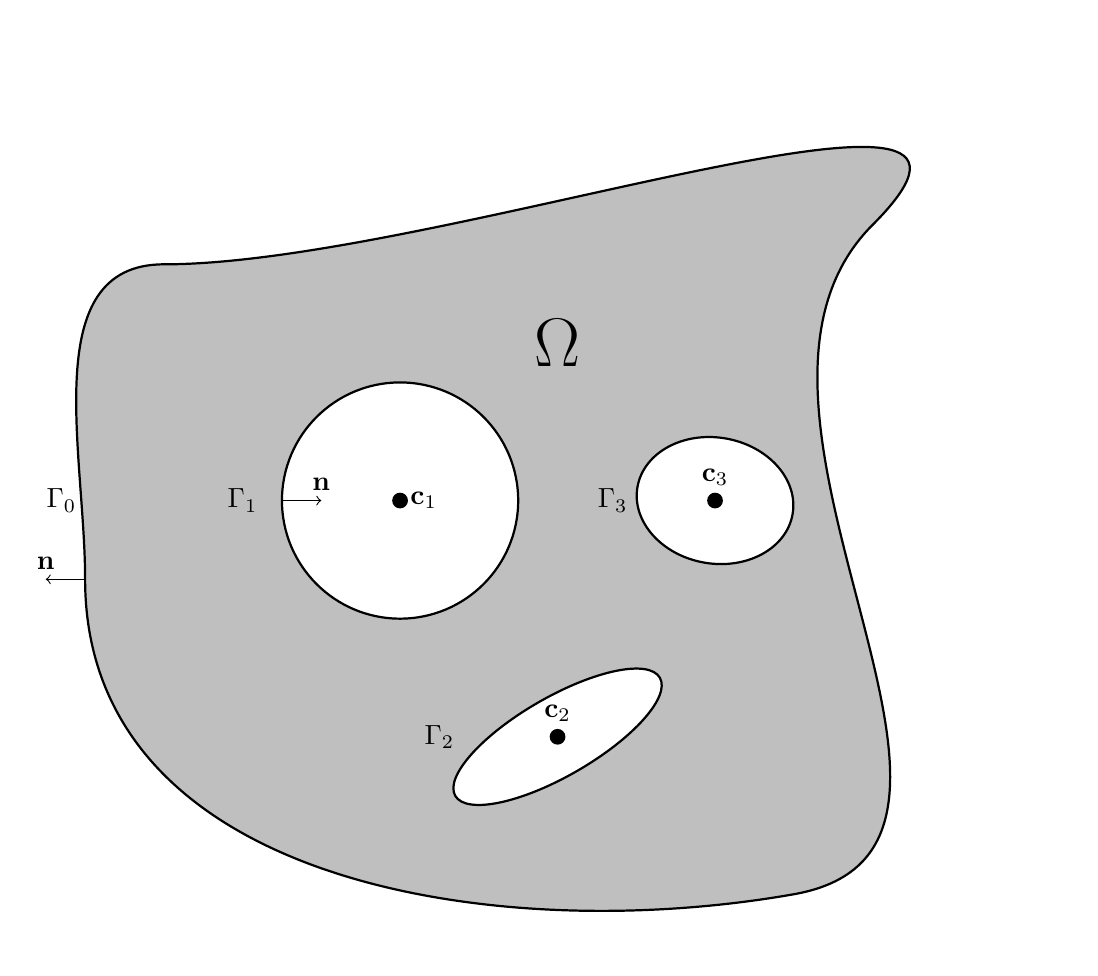
\begin{tikzpicture}
	\path[fill=lightgray, draw=black, thick]
	 (-2,0) to [out=90,in=180](-1,4) to[out=0, in = 45](8,4.5) to[out=225, in=10](7,-4) to[out=190, in=270](-2,0);
	\draw[thick, fill=white] (2,1) circle(1.5);
	\draw[thick, fill=white] (4,-2)[rotate around={30:(4,-2)}]circle[x radius=1.5, y radius = 0.5];
	\draw[thick, fill=white] (6,1)[rotate around={-10:(6,1)}]circle[x radius=1, y radius = 0.8];
	\fill(2,1)circle(0.1);
	\fill(6,1)circle(0.1);
	\fill(4,-2)circle(0.1);
	\draw(2.3,1) node {$\mathbf{c}_1$};
	\draw(4,-1.7) node {$\mathbf{c}_2$};
	\draw(6,1.3) node {$\mathbf{c}_3$};
	\draw(4,3) node {\Huge$\Omega$};
	\draw(-2.3,1) node {$\Gamma_0$};
	\draw(0,1) node {$\Gamma_1$};
	\draw(2.5,-2) node {$\Gamma_2$};
	\draw(4.7,1) node {$\Gamma_3$};
	\draw[->](0.5,1)--(1,1) node[align=center, above]{$\mathbf{n}$};
	\draw[->](-2,0)--(-2.5,0) node[align=center, above]{$\mathbf{n}$};
\end{tikzpicture}
\end{center}
\caption[Sketch of an admissible domain.]{Sketch of three-ply connected domain. In this case $\partial\Omega$ is the union of $\Gamma_0$, $\Gamma_1$, $\Gamma_2$ and $\Gamma_3$. $\Gamma_0$ is always the enclosing boundary. The point $\mathbf{c}_k$, $k=1, 2, 3$ is an arbitrary point inside obstacle $k$.}\label{fig:omega_bounded}
\end{figure}


\section{Completed Double Layer Potential}


The fundamental solution of the Stokes equations in $\mathbb{R}^2$, $\{\pmb{\Phi}^k(\mathbf{x},\mathbf{y}),\psi^k(\mathbf{x},\mathbf{y})\}$, $k = 1,2$ satisfies
\begin{align*}
	\Delta_{\mathbf{x}}\pmb{\Phi}^k(\mathbf{x},\mathbf{y}) - \nabla_{\mathbf{x}}\psi^k(\mathbf{x},\mathbf{y}) &= \delta(\mathbf{x}-\mathbf{y})\mathbf{e}^k,\\
	\nabla_{\mathbf{x}} \cdot\pmb{\Phi}^k = 0.
\end{align*}
where $\mathbf{e}^k$ is the unit vector in direction $k$ and $\delta(\mathbf{x}-\mathbf{y})$ is the Dirac delta function centered at $\mathbf{y}$. The fundamental solution is given by
\begin{comment}
\begin{align*}
	\pmb{\Phi}(x_1,x_2,y_1,y_2) &= \frac{1}{4\pi}\tiny\begin{pmatrix} (x_1 - y_1)(x_1 - y_1) - \ln\left(\sqrt{(x_1 - y_1)^2+(x_2-y_2)^2}\right) & (x_1 - y_1)(x_2-y_2) \\  (x_1 - y_1)(x_2-y_2) &  (x_2 - y_2)(x_2 - y_2) - \ln\left(\sqrt{(x_1 - y_1)^2+(x_2-y_2)^2}\right) \end{pmatrix}\\
	\pmb{\psi}(x_1,x_2,y_1,y_2) &=\frac{1}{\pi} \begin{pmatrix} \frac{x_1 - y_1}{\sqrt{(x_1 - y_1)^2+(x_2-y_2)^2}} \\  \frac{x_2 - y_2}{\sqrt{(x_1 - y_1)^2+(x_2-y_2)^2}}\end{pmatrix}
\end{align*}
Equivalently, in more compact notation
\end{comment}
\begin{subequations}
\begin{align}
	\pmb{\Phi}(\mathbf{x},\mathbf{y}) &= \frac{1}{4\pi}\left(\frac{\mathbf{r}\otimes\mathbf{r}}{\rho^2} - \ln\rho\mathbf{I}\right),\\
	\pmb{\psi}(\mathbf{x},\mathbf{y}) &= \frac{1}{\pi}\left(\frac{\mathbf{r}}{\rho^2}\right),
\end{align}
\end{subequations}
where $\mathbf{r} = \mathbf{x} - \mathbf{y}$ is the vector joining the target point $\mathbf{x}\in\Omega$ to the source point $\mathbf{y}\in\Omega$ and $\rho = |\mathbf{r}|$ is its length. The fundamental solution for the velocity is known as a \textit{Stokeslet} and represents the fluid velocity at $\mathbf{x}$ induced by a point force of unit strength at $\mathbf{y}$. 

\begin{comment}
From the Stokeslet, we can obtain the double layer potentials
\begin{subequations}
\begin{align}
	 \mathcal{D}[\pmb{\eta}](\mathbf{x}) &= \int_{\partial\Omega} \left(\sigma_{ij}(\pmb{\Phi}^k)n_k\right)\eta_i(\mathbf{y})\text{d}\mathbf{y} =  \int_{\partial\Omega} \mathbf{W}\pmb{\eta}(\mathbf{y})\text{d}\mathbf{y}, \label{eq:dlp_u}\\
	\mathcal{C}[\pmb{\eta}](\mathbf{x}) &= \int_{\partial\Omega} \frac{\partial \psi^k}{\partial x_j}n_j\eta_k(\mathbf{y})\text{d}\mathbf{y} = \int_{\partial\Omega}\mathbf{q}\cdot\pmb{\eta}(\mathbf{y})\text{d}\mathbf{y},
\end{align}
\end{subequations}
where $\eta(\mathbf{y}) = \langle \eta_1(\mathbf{y}), \eta_2(\mathbf{y})\rangle$ is an unknown density function and $\sigma_{ij}(\pmb{\Phi}^k)$ is called the \textit{stresslet}, given by:
\begin{equation}
	\sigma_{ij}\left(\pmb{\Phi}^k(\mathbf{x},\mathbf{y})\right) = \mathbf{I}\pmb{\psi} + \left(\nabla_{\mathbf{x}}\pmb{\Phi}^k + \nabla_{\mathbf{x}} \left(\pmb{\Phi^k}\right)^T\right).
\end{equation}


This leads to the kernels of the double layer potentials
\begin{subequations}
\begin{align}
	\mathbf{W}(\mathbf{x},\mathbf{y}) & = -\frac{1}{\pi}\left(\frac{\mathbf{r}\cdot\mathbf{n}}{\rho^4}\mathbf{r}\otimes\mathbf{r}\right),\label{eq:dlp_u_kernel}\\
		\mathbf{q}(\mathbf{x},\mathbf{y}) &= \frac{1}{\pi}\nabla_x \left(\frac{\mathbf{r}\cdot\mathbf{n}}{\rho^2}\right).
\end{align}
\end{subequations}
\end{comment}

The stress tensor arising from the fundamental solution,
\[ \mathbf{T}(\mathbf{x},\mathbf{y}) = -\psi \mathbf{I} + \left(\nabla_{\mathbf{x}} \pmb{\Phi} + \left(\nabla_{\mathbf{x}}\pmb{\Phi}\right)^T\right),\]
can be used to create the kernel for the \textit{double layer potential},
\begin{equation}\label{eq:dlp_u} \mathcal{D}[\pmb{\eta}](\mathbf{x}) = \int_{\partial\Omega} \mathbf{K}(\mathbf{x},\mathbf{y})\pmb{\eta}(\mathbf{y})\text{d}s(\mathbf{y}),\end{equation}
where $\mathbf{K}(\mathbf{x},\mathbf{y}) = -\mathbf{T}(\mathbf{x},\mathbf{y})\hat{\mathbf{n}}(\mathbf{y})$, with $\hat{\mathbf{n}}$ being the unit normal pointing out of the fluid domain. 


To set up a Fredhom integral equation we will look at the limit of \eqref{eq:dlp_u} as $\mathbf{x}$ approaches a point  $\mathbf{x}^*\in\partial\Omega$. The double layer kernel has a jump as we cross the boundary, and this leads to a discontinuity in the double layer potential \cite{Ladyzhenskaya1963},
\begin{subequations}\label{eq:dlp_limits}
\begin{align}
	\lim_{\substack{ \mathbf{x}\to\mathbf{x}^*\\ \mathbf{x}\notin \Omega}} \mathcal{D}[\pmb{\eta}](\mathbf{x})= \frac{1}{2}\pmb{\eta}(\mathbf{x}^*) &+ \int_{\partial\Omega} \mathbf{K}(\mathbf{x}^*,\mathbf{y})\pmb{\eta}(\mathbf{y})\text{d}s(\mathbf{y}), \\
\lim_{\substack{ \mathbf{x}\to\mathbf{x}^*\\ \mathbf{x}\in \Omega}} \mathcal{D}[\pmb{\eta}](\mathbf{x})= -\frac{1}{2}\pmb{\eta}(\mathbf{x}^*) &+ \int_{\partial\Omega} \mathbf{K}(\mathbf{x}^*,\mathbf{y})\pmb{\eta}(\mathbf{y})\text{d}s(\mathbf{y}).
\end{align}
\end{subequations}

\begin{figure}[!h]
\begin{tabular}{c c}
	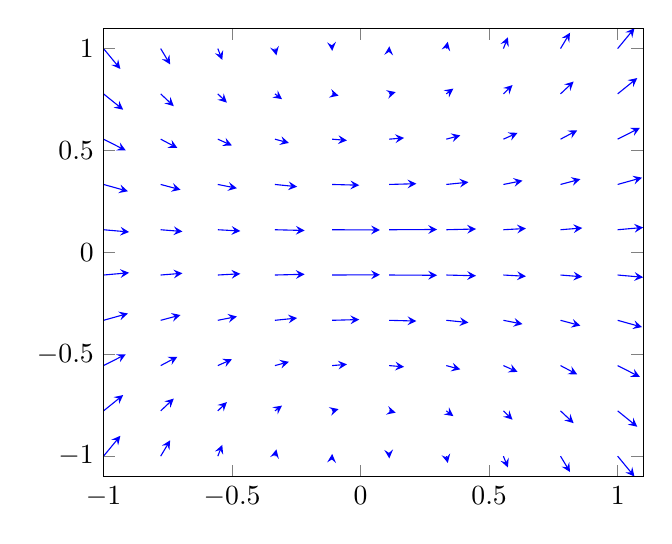
\begin{tikzpicture}
	\begin{axis}[domain=-1:1, view={0}{90}]
	\addplot3[blue, quiver={u={x^2-ln(sqrt(x^2+y^2)}, v={x*y}, scale arrows=0.1}, -stealth,samples=10] {0};
	\end{axis}
	\end{tikzpicture}
&
	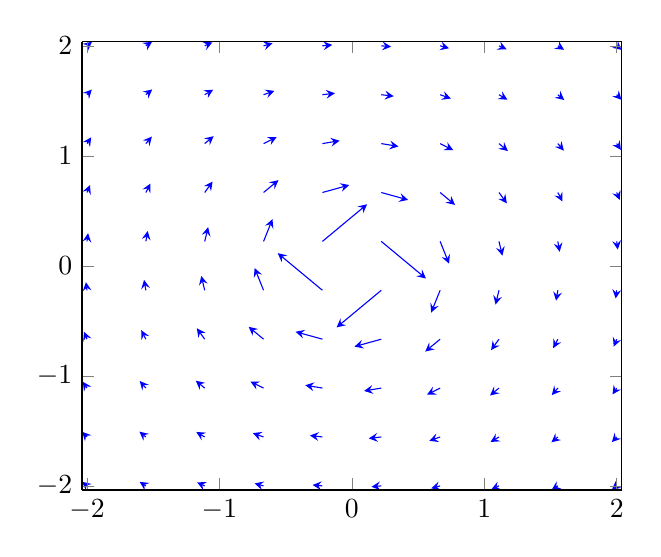
\begin{tikzpicture}
	\begin{axis}[domain=-2:2, view={0}{90}]
	\addplot3[blue, quiver={u={y/(x^2+y^2)}, v={-x/(x^2+y^2)}, scale arrows=0.15}, -stealth,samples=10] {0};
	\end{axis}
	\end{tikzpicture}
\end{tabular}
\caption[Plots of Stokeslet and rotlet.]{Example of singularities centered at origin. Left: Stokeslet.  Right:  Rotlet.}\label{fig:singularity}
\end{figure}

By setting the velocity field to the double layer potential, the goal becomes to match the Dirichlet boundary conditions \eqref{eq:u_bc} with the appropriate limiting value in \eqref{eq:dlp_limits}. This  leads to  the integral equation
\begin{equation}\label{eq:fredholm_sing} - \frac{1}{2}\pmb{\eta}(\mathbf{x}) + \mathcal{D}[\pmb{\eta}](\mathbf{x}) = \mathbf{U}\qquad \mathbf{x}\in\partial\Omega.\end{equation}
This is a desirable Fredholm equation of the second kind for the unknown density function $\pmb{\eta}$ defined on $\partial\Omega$. 


Unfortunately, defining the velocity in terms of just the double layer potential does not let us represent every possible flow field. In particular we are limited to problems where the net force and torque on the boundary is 0. Thus \eqref{eq:fredholm_sing} is solvable only if this condition is met. This necessitates the completion~\cite{Power1993, Power1987} of the double layer potential by adding linear combinations of \textit{rotlets}, given by
\begin{equation}
	\mathbf{R}(\mathbf{x},\mathbf{y})\xi = \xi\frac{\mathbf{r}^\perp}{\rho^2},
\end{equation}
and Stokeslets for each obstacle in the domain. For notational purposes we will write Stokeslets as
\[ \mathbf{S}(\mathbf{x},\mathbf{y})\pmb{\lambda} = \pmb{\Phi}(\mathbf{x},\mathbf{y})\pmb{\lambda}.\]
Rotlets are the rotational analogue of Stokeslets and represent the fluid velocity induced by a point torque. Stokeslets and rotlets are called \textit{singularities}; an example of a Stokeslet and a rotlet are shown in Figure \ref{fig:singularity}. The Stokeslet $\mathbf{S}(\mathbf{x},\mathbf{c}_k)\pmb{\lambda}_k$ centered  inside obstacle $k$ exerts a total force $\pmb{\lambda}_k$ on obstacle $k$, and zero total torque. The rotlet $\mathbf{R}(\mathbf{x},\mathbf{c}_k)\xi_k$ centered inside obstacle $k$ exerts zero total force on obstacle $k$ and total torque equal to $\xi_k$. 

By adding in the Rotlets and Stokeslets we arrive at the \textit{completed double layer potential}
\begin{equation}\label{eq:dlp_complete}
	 \mathbf{u}(\mathbf{x}) = \mathcal{D}[\pmb{\eta}](\mathbf{x}) + \sum\limits_{k=1}^n\mathbf{S}(\mathbf{x},\mathbf{c}_k)\pmb{\lambda}_k + \sum\limits_{k=1}^n \mathbf{R}(\mathbf{x},\mathbf{c}_k)\xi_k,\end{equation}
where $\mathbf{c}_k$, $k=1,\hdots,n$ is a point inside obstacle $k$, as shown in figure \ref{fig:omega_bounded}. Typically this will be the center of the obstacle, but this is not necessary. Since  the double layer potential does not exert any force or torque on a closed surface, the total force on obstacle $k$ is $\pmb{\lambda}_k$ and the total torque exerted on obstacle $k$ is $\xi_k$. 



At this point we have more unknowns than equations. One way to close the system is to relate the total force on each obstacle $\pmb{\lambda}_k$ and the total torque on each obstacle $\xi_k$ to the density $\pmb{\eta}$ by
\begin{subequations}\label{eq:constraints}
\begin{align}
	\pmb{\lambda}_k &= \frac{1}{2\pi} \int_{\Gamma_k} \pmb{\eta}(\mathbf{y}) \text{d}s,\label{eq:force}\\
	\xi_k &= \frac{1}{2\pi}\int_{\Gamma_k}\left( (\mathbf{y} - \mathbf{c}_k)^\perp \cdot\pmb{\eta}(\mathbf{y})\right)\text{d}s. \label{eq:torque}
\end{align}
\end{subequations}

To finish our discussion of the completed double layer potential, we note that  $\int_{\Gamma_0} \mathbf{u}\cdot\mathbf{n}\text{d}s = 0$ implies that $\int_{\Gamma_0 }\pmb{\eta}\cdot\mathbf{n}\text{d}s = 0$~\cite{Pozrikidis1992}. By the Fredholm alternative, this constraint means that we have a rank one null space. It can be removed by adding an additional operator that is active along the boundary $\Gamma_0$
\begin{equation}
	\mathcal{N}_0[\pmb{\eta}](\mathbf{x}) = \int_{\Gamma_0}(\hat{\mathbf{n}}(\mathbf{x})\otimes\hat{\mathbf{n}}(\mathbf{y}))\pmb{\eta}(\mathbf{y})\text{d}s(\mathbf{y}).
\end{equation}

\section{Canonical Equations for Resistance and Mobility Problems}

There are two common types of problems this formulation allows us to solve. The first is the \textit{resistance problem}, where the velocity of each obstacle is specified  and we are tasked with computing the forces and torques on each particle. The other problem, in which the forces and torques on the obstacles are specified and we must compute the velocity is called the \textit{mobility problem}. 

Assuming no-slip boundary conditions, we have
\begin{equation}\label{eq:canonical1}
-\frac{1}{2}\pmb{\eta}(\mathbf{y}) + \mathcal{D}[\pmb{\eta}](\mathbf{y}) + \sum\limits_{j=1}^n \biggr(\mathbf{S}(\mathbf{y},\mathbf{c}_j)\pmb{\lambda}_j + \mathbf{R}(\mathbf{y},\mathbf{c}_j)\xi_j\biggr) + \delta_{0k}\mathcal{N}_0[\pmb{\eta}](\mathbf{y}) = \mathbf{U}(\mathbf{y}) \qquad \text{for } \mathbf{y}\in\Gamma_k.
\end{equation}

The velocity on $\Gamma_k$ can be decomposed into a translational velocity $\mathbf{U}^\tau_k$ and a rotational velocity $\omega_k$:
\[ \mathbf{U}(\mathbf{y}) = \mathbf{U}^\tau_k + \omega_k(\mathbf{y} - \mathbf{c}_k)^\perp \qquad \mathbf{y}\in\Gamma_k.\]

Using this decomposition in \eqref{eq:canonical1} and adding the constraints \eqref{eq:constraints} yields our final system
\begin{subequations}\label{eq:canonical}
\begin{equation}\label{eq:canonical_a}
\begin{aligned}
	 \mathbf{U}^\tau_k + \omega_k(\mathbf{x} - \mathbf{c}_k)^\perp &= -\frac{1}{2}\pmb{\eta}(\mathbf{x}) + \mathcal{D}[\pmb{\eta}](\mathbf{x}) \\+ &\sum\limits_{j=1}^n \mathbf{S}(\mathbf{x},\mathbf{c}_j)\pmb{\lambda}_j + \mathbf{R}(\mathbf{x},\mathbf{c}_j)xi_j + \delta_{0k}\mathcal{N}_0[\pmb{\eta}](\mathbf{x}) \qquad \mathbf{x}\in\Gamma_k,
\end{aligned}
\end{equation}
\begin{align}
	\pmb{\lambda}_k &= \frac{1}{2\pi} \int_{\Gamma_k} \pmb{\eta}(\mathbf{y}) \text{d}s,\\
	\xi_k &= \frac{1}{2\pi}\int_{\Gamma_k} (\mathbf{y} - \mathbf{c}_k)^\perp \cdot\pmb{\eta}(\mathbf{y})\text{d}s.
\end{align}
\end{subequations}

These are the canonical equations \cite{Karrila1989} for the resistance and mobility problem. Here for each $k = 1,\hdots, n$ we must specify either the velocity $\mathbf{U}(\mathbf{y}) = \mathbf{U}_\tau + \omega(\mathbf{y} - \mathbf{c}_k)^\perp$, or the net force $\pmb{\lambda_k}$ and torque $\xi_k$ along $\Gamma_k$. We then solve for the other variables, including the density function $\pmb{\eta}$.

\section{Computational Considerations}

Consider a domain bounded by $\Gamma_0$ containing $N + M$ total obstacles: $M $ of type 1, on which we specify the velocity $\mathbf{U}$ and $N$ of type 2, on which we specify the total force $\pmb{\lambda}$ and torque $\xi$. The outer boundary as well as obstacles of type 1 will be called solid walls, while the obstacles of type 2 will be called particles. Define:
\[ \Gamma_w = \bigcup\limits_{k=1}^M \Gamma_k, \qquad\qquad \Gamma_p = \bigcup\limits_{k=M+1}^{N+M} \Gamma_k.\]

An example of such a domain, with $N=4$ and $M=1$ is shown in Figure \ref{fig:couette}. We wish to solve for the total force and torque on $\Gamma_0 \cup \Gamma_w$ and the translational and angular velocity on $\Gamma_p$. 

\begin{figure}[!h]
\begin{center}
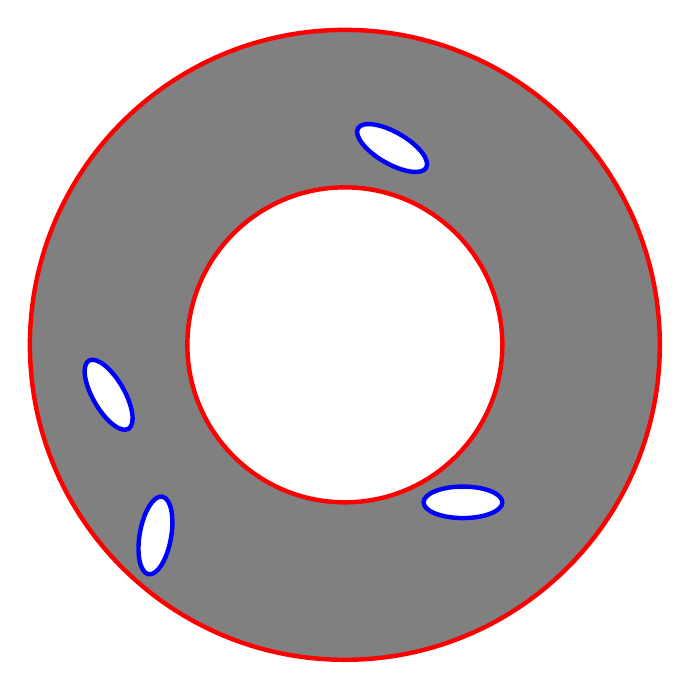
\begin{tikzpicture}
	\draw[ultra thick, red, fill=gray] (5,5) circle(4);
	\draw[ultra thick, red,  fill=white] (5,5) circle(2);
	\draw[ultra thick, blue, fill=white] (2.5,2.5)[rotate around={-10:(3,2)}]circle[x radius=0.2, y radius = 0.5];
	\draw[ultra thick, blue, fill=white] (2.5,4.5)[rotate around={30:(2.5,3.5)}]circle[x radius=0.2, y radius = 0.5];
	\draw[ultra thick, blue, fill=white] (6.5,3)[rotate around={90:(6.5,3)}]circle[x radius=0.2, y radius = 0.5];
	\draw[ultra thick, blue, fill=white] (5.6,7.5)[rotate around={60:(5.6,7.5)}]circle[x radius=0.2, y radius = 0.5];
\end{tikzpicture}
\end{center}
\caption[Sketch of a Couette device.]{Sketch of a Couette device. Objects outlined in red are solid walls;  objects outlined in blue are suspended particles.}\label{fig:couette}
\end{figure}

To simplify the calculations we will make use of the \textit{quasi-static approximation}. This approximation is commonly used in low Reynolds number particle simulations. Under this approximation the particles instantaneously adjust their velocities to assume a force-free configuration \cite{Kropinski1997}. This allows us to evaluate the  evolution of the particles by solving a sequence of steady problems of the form \eqref{eq:stokes}. 

Splitting the integrals in \eqref{eq:canonical_a} into integrals along the walls and integrals along particles and applying the quasi-static approximation gives
\begin{subequations}\label{eq:int_split}
\begin{equation}
\begin{aligned} 
-\frac{1}{2}\pmb{\eta}_p(\mathbf{x}) + \mathcal{D}[\pmb{\eta}_p](\mathbf{x}) &+ \mathcal{D}[\pmb{\eta}_w](\mathbf{x}) + \sum\limits_{j=1}^m \biggr(\mathbf{S}(\mathbf{x},\mathbf{c}_j)\pmb{\lambda}_j + \mathbf{R}(\mathbf{x},\mathbf{c}_j)\xi_j\biggr)\\& - \mathbf{U}(\mathbf{x}) - \omega(\mathbf{x}-\mathbf{c}_k)^\perp = 0 \qquad \mathbf{x}\in \Gamma_p,
\end{aligned}
\end{equation}
\begin{equation}
\begin{aligned} 
-\frac{1}{2}\pmb{\eta}_w(\mathbf{x}) + \mathcal{D}[\pmb{\eta}_p](\mathbf{x}) &+ \mathcal{D}[\pmb{\eta}_w](\mathbf{x}) + \sum\limits_{j=1}^m \biggr(\mathbf{S}(\mathbf{x},\mathbf{c}_j)\pmb{\lambda}_j + \mathbf{R}(\mathbf{x},\mathbf{c}_j)\xi_j\biggr) \\&= \mathbf{U}(\mathbf{x}) + \omega(\mathbf{x}-\mathbf{c}_k)^\perp \qquad \mathbf{x}\in \Gamma_w,
\end{aligned}
\end{equation}
\begin{equation}
\begin{aligned} 
-\frac{1}{2}\pmb{\eta}_w(\mathbf{x}) + \mathcal{D}[\pmb{\eta}_p](\mathbf{x}) &+ \mathcal{D}[\pmb{\eta}_w](\mathbf{x}) + \sum\limits_{j=1}^m \biggr(\mathbf{S}(\mathbf{x},\mathbf{c}_j)\pmb{\lambda}_j + \mathbf{R}(\mathbf{x},\mathbf{c}_j)\xi_j\biggr) \\& + \mathcal{N}_0[\pmb{\eta}_w](\mathbf{x}) = \mathbf{U}(\mathbf{x}) + \omega(\mathbf{x}-\mathbf{c}_k)^\perp \qquad \mathbf{x}\in \Gamma_0.
\end{aligned}
\end{equation}

\end{subequations}

\subsection{Discretization}


The equations \ref{eq:canonical} and \eqref{eq:int_split} can be written in the compact form
 \begin{subequations}\label{eq:compact}
\begin{alignat}{3}
	\mathbf{V}_{dlp} + \mathbf{V}_{s,r} - \mathbf{V}_{p} &= \mathbf{0} \qquad &&\text{ on } \Gamma_p,\\
	\mathbf{V}_{dlp} + \mathbf{V}_{s,r} &= \mathbf{V}_{w} \qquad &&\text{ on } \Gamma_w,\\
	\mathbf{F}_{\pmb{\eta}} - \mathbf{F}_{s,r} &= \mathbf{0} \qquad &&\text{ on } \Gamma_w,
\end{alignat}
\end{subequations}
where $\mathbf{V}_{dlp}$ is the velocity induced by the double layer potential, $\mathbf{V}_{s,r}$ is the velocity induced by the Stokeslets and Rotlets, $\mathbf{V}_p$ is the unknown particle velocity and $\mathbf{V}_w$ is the prescribed wall velocity. $\mathbf{F}_{s,r}$ is the net force and torque generated by the Rotlets and Stokeslets on each of the walls, and $\mathbf{F}_{\pmb{\eta}}$ is the net force and torque generated by the density function $\pmb{\eta}$ on each of the walls. 

To discretize the integrals in the \eqref{eq:compact}, we will use the collocation method discussed in Section \ref{sec:discretization}. Specifically we will use the trapezoid rule, which is spectrally accurate for $C^\infty$ periodic integrands such as ours. The integrals around each of the $n$ particles will be discretized using $J$ points, and the integrals around each of the $M$ walls will be discretized using $L$ points. This leads to $2(NJ + ML)$ unknowns for the density function $\pmb{\eta}$, plus an additional $3$ unknowns (translational and rotational velocities or forces and torques) for each boundary (except $\Gamma_0$). Thus the total number of unknowns is $2(NJ + ML) + 3(N+M - 1)$. 

We first parameterize the walls and particles from $0$ to $2\pi$. The spacing between discretization points on the particles, $h_{p}$, is then $2\pi/J$ and the spacing between points on the walls, $h_w$ is $2\pi/L$. Each point, $\mathbf{y}^k_i$ is associated with an unknown density $\pmb{\eta}^k_i$.

At a point $\mathbf{y}^k_i$ on particle $k$, we can discretize $\mathbf{V}_{dlp}$ as
\begin{equation}\label{eq:vdlp}
\begin{aligned}
\mathbf{V}_{dlp}(\mathbf{y}^k_i) = -\frac{1}{2}\pmb{\eta}^k_i  +h_p\bigg( &\sum_{\substack{j=1\\j\ne i}}^J \mathbf{K}_k(\mathbf{y}^k_j,\mathbf{y}^k_i)\pmb{\eta}_j^k +\frac{\kappa_k(\mathbf{y}^k_i)}{2}(\pmb{\tau}(\mathbf{y}^k_i)\otimes\pmb{\tau}(\mathbf{y}_i^k))\pmb{\eta}_i^k\bigg) \\&+ h_p\sum\limits_{\substack{n=1\\n\ne k}}^N\sum\limits_{j=1}^J  \mathbf{K}_n(\mathbf{y}^n_j,\mathbf{y}^k_i)\pmb{\eta}_j^n  + h_w \sum\limits_{m=1}^M\sum\limits_{\ell=1}^L \mathbf{K}_m(\mathbf{y}^m_\ell,\mathbf{y}^k_i)\pmb{\eta}^m_\ell .
\end{aligned}
\end{equation}
 
The first summation in \eqref{eq:vdlp} is the self contribution to the velocity at $\mathbf{y}^k_i$, that is, the velocity due to all other points on particle $k$. The kernel in the double layer potential has a removable singularity at $\mathbf{x}=\mathbf{y}$, so self-self summation skips the entry $j=i$. It is replaced by its limiting value, which involves the curvature of the boundary $\kappa$, and the tangential vectors $\pmb{\tau}$ \cite{Ladyzhenskaya1963}. 

The second summation is the contribution due to all other particles. The last summation is the wall contribution, which is the velocity at $\mathbf{y}^k_i$ due to points on the walls. The kernels have all been modified slightly to account for the mapping from the boundary to the interval $[0,2\pi]$. The modified kernel $\mathbf{K}_n$ is defined to be
\[ \mathbf{K}_n(\mathbf{x},\mathbf{y}) = \mathbf{K}(\mathbf{x},\mathbf{y})||\mathbf{r}_n'(\mathbf{y})||,\]
where $\mathbf{r}_n(\mathbf{y})$ is a parameterization of $\Gamma_n$. A similar expression can be given for $\mathbf{V}_{dlp}$ evaluated on the walls, with the addition of $\mathcal{N}_0[\pmb{\eta}]$ on $\Gamma_0$. 

To solve the linear system \eqref{eq:compact} we will use the iterative solver \textit{generalized minimum residual method} (GMRES)~\cite{Saad1986}. This is a Krylov solver that does not require the matrix to have any special properties. GMRES works best for problems arising from compact operators with eigenvalues clustered away from the origin ~\cite{Rasmussen2001}, which due to fact that the completed double layer potential is a Fredholm equation of the second kind, is satisfied by our problem. In this case we expect the number of GMRES iterations to be independent of the mesh resolution. Computing the sums in \eqref{eq:vdlp} directly requires $O(N^2)$  time ($N$ here being the total number of points). This can be sped up to $O(N)$ by using an approximate summation technique known as the \textit{fast multipole method} (FMM)~\cite{Greengard1987, Nishimura2002}. To perform the FMM we use a Fortran library provided by Leslie Greengard and Manas Rachh that can be run in parallel using OpenMP. 


\subsection{Near Singular Integration}\label{sec:near_singular}



Although the kernel of the double layer potential is $C^{\infty}$ continuous, its derivative grows as the source and target points become close.

 Consider the scenario in Figure \ref{fig:near_experiment}. As $x_2$ approaches the top of the unit circle, the integrand becomes more singular. Once $x_2$ hits the top of the circle the integrand becomes smooth as it takes the limiting value which depends on the curvature and the tangential vectors. The errors and convergence rates of the trapezoid rule are in Table \ref{table:near_singular} for various grid resolutions. As expected, the integrand becomes more singular and the error in the trapezoid rule increases.

\begin{figure}[!h]
\begin{tabular}{cc}
\begin{tikzpicture}
	\draw[white](0,-2) -- (1.5,-2);
	\draw[thick] (0,2) circle(2);
	\draw[thick] (0,5) node[cross=4pt] {};
	\draw(3.5,2) node {$\mathbf{r}_1(t) = \begin{pmatrix} \cos(\theta)\\ \sin(\theta)\end{pmatrix}$};
	\draw(0.5,5.5) node {$\mathbf{x} =\begin{pmatrix}0\\ x_2\end{pmatrix}$};
\end{tikzpicture}
&
% This file was created by matlab2tikz.
%
%The latest updates can be retrieved from
%  http://www.mathworks.com/matlabcentral/fileexchange/22022-matlab2tikz-matlab2tikz
%where you can also make suggestions and rate matlab2tikz.
%
\documentclass[tikz]{standalone}

\usepackage[T1]{fontenc}
\usepackage[utf8]{inputenc}
\usepackage{pgfplots}
\usepackage{grffile}
\pgfplotsset{compat=newest}
\usetikzlibrary{plotmarks}
\usepgfplotslibrary{patchplots}
\usepackage{amsmath}
\usetikzlibrary{decorations.markings}
\usetikzlibrary{decorations, decorations.text,backgrounds}
\usetikzlibrary{spy}
\usetikzlibrary{shapes.misc}
\usetikzlibrary{external}
\usetikzlibrary{backgrounds}

\tikzset{cross/.style={cross out, draw=black, minimum size=2*(#1-\pgflinewidth), inner sep=0pt, outer sep=0pt},cross/.default={1pt}}

\begin{document}


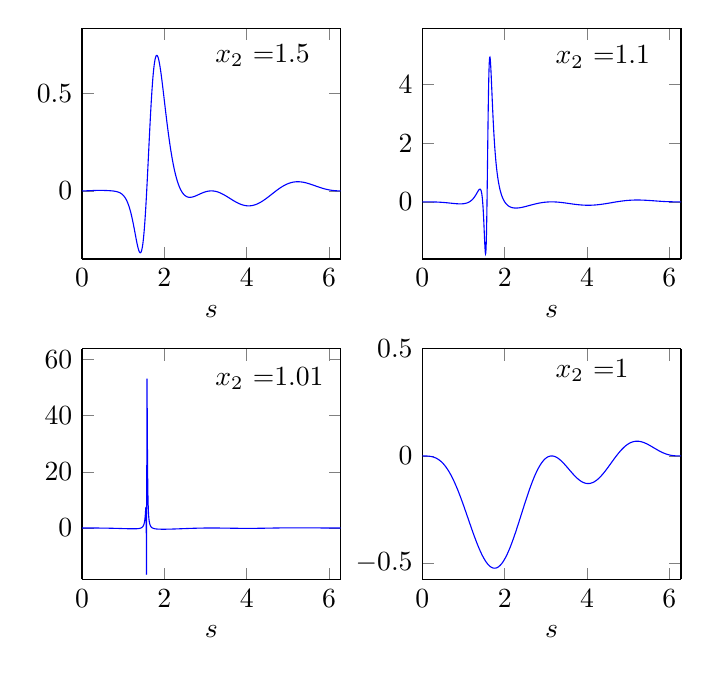
\begin{tikzpicture}

\begin{axis}[%
width=3.285cm,
height=2.93cm,
at={(0cm,4.07cm)},
scale only axis,
separate axis lines,
every outer x axis line/.append style={black},
every x tick label/.append style={font=\color{black}},
xmin=0,
xmax=6.28318530717959,
xlabel={$s$},
every outer y axis line/.append style={black},
every y tick label/.append style={font=\color{black}},
ymin=-0.349426375257459,
ymax=0.835179397146845,
axis background/.style={fill=white}
]
\addplot [color=blue,solid,forget plot]
  table[row sep=crcr]{%
0	0\\
0.00628947478196155	1.85301227206507e-006\\
0.0125789495639231	7.33350376875469e-006\\
0.0188684243458846	1.63227596802755e-005\\
0.0251578991278462	2.87009483862605e-005\\
0.0314473739098077	4.43472208741606e-005\\
0.0377368486917693	6.31398109613263e-005\\
0.0440263234737308	8.49561362572533e-005\\
0.0503157982556924	0.000109672899800723\\
0.0566052730376539	0.000137166192304791\\
0.0628947478196155	0.000167311594940741\\
0.069184222601577	0.000199984282590282\\
0.0754736973835386	0.000235059127493316\\
0.0817631721655001	0.000272410803216679\\
0.0880526469474617	0.000311913888867223\\
0.0943421217294232	0.00035344297347055\\
0.100631596511385	0.000396872760434586\\
0.106921071293346	0.000442078172015008\\
0.113210546075308	0.000488934453697278\\
0.119500020857269	0.000537317278407747\\
0.125789495639231	0.000587102850463911\\
0.132078970421193	0.000638168009171435\\
0.138368445203154	0.000690390331973068\\
0.144657919985116	0.000743648237051939\\
0.150947394767077	0.000797821085289036\\
0.157236869549039	0.000852789281471927\\
0.163526344331	0.000908434374648872\\
0.169815819112962	0.000964639157519546\\
0.176105293894923	0.00102128776475049\\
0.182394768676885	0.00107826577010029\\
0.188684243458846	0.00113546028223617\\
0.194973718240808	0.00119276003912022\\
0.20126319302277	0.00125005550084017\\
0.207552667804731	0.00130723894075568\\
0.213842142586693	0.0013642045348276\\
0.220131617368654	0.00142084844899361\\
0.226421092150616	0.00147706892444957\\
0.232710566932577	0.00153276636069173\\
0.239000041714539	0.0015878433961706\\
0.2452895164965	0.00164220498640276\\
0.251578991278462	0.001695758479382\\
0.257868466060423	0.00174841368812649\\
0.264157940842385	0.00180008296019362\\
0.270447415624347	0.00185068124398851\\
0.276736890406308	0.00190012615168724\\
0.28302636518827	0.00194833801858975\\
0.289315839970231	0.00199523995871151\\
0.295605314752193	0.00204075791641706\\
0.301894789534154	0.00208482071389197\\
0.308184264316116	0.00212736009424322\\
0.314473739098077	0.00216831076001093\\
0.320763213880039	0.00220761040686753\\
0.327052688662	0.00224519975227253\\
0.333342163443962	0.00228102255884369\\
0.339631638225924	0.0023150256521972\\
0.345921113007885	0.00234715893300104\\
0.352210587789847	0.00237737538297704\\
0.358500062571808	0.00240563106457824\\
0.36478953735377	0.00243188511405849\\
0.371079012135731	0.00245609972764185\\
0.377368486917693	0.00247824014048892\\
0.383657961699654	0.00249827459814685\\
0.389947436481616	0.00251617432015896\\
0.396236911263578	0.00253191345549842\\
0.402526386045539	0.00254546902947881\\
0.408815860827501	0.00255682088178233\\
0.415105335609462	0.00256595159523353\\
0.421394810391424	0.00257284641493363\\
0.427684285173385	0.00257749315735688\\
0.433973759955347	0.00257988210899648\\
0.440263234737308	0.00258000591413285\\
0.44655270951927	0.00257785945128235\\
0.452842184301231	0.00257343969786896\\
0.459131659083193	0.00256674558264533\\
0.465421133865155	0.00255777782537314\\
0.471710608647116	0.0025465387632559\\
0.478000083429078	0.00253303216359923\\
0.484289558211039	0.00251726302215624\\
0.490579032993001	0.00249923734659646\\
0.496868507774962	0.00247896192451783\\
0.503157982556924	0.0024564440754018\\
0.509447457338885	0.00243169138589108\\
0.515736932120847	0.00240471142774914\\
0.522026406902809	0.00237551145783939\\
0.52831588168477	0.00234409809944033\\
0.534605356466732	0.00231047700419094\\
0.540894831248693	0.00227465249393824\\
0.547184306030655	0.00223662718173582\\
0.553473780812616	0.00219640157121953\\
0.559763255594578	0.00215397363356262\\
0.566052730376539	0.00210933836118915\\
0.572342205158501	0.00206248729740095\\
0.578631679940462	0.0020134080410491\\
0.584921154722424	0.00196208372535743\\
0.591210629504386	0.00190849246998172\\
0.597500104286347	0.00185260680536457\\
0.603789579068309	0.00179439306842306\\
0.61007905385027	0.0017338107685835\\
0.616368528632232	0.00167081192315561\\
0.622658003414193	0.00160534036101725\\
0.628947478196155	0.00153733099356098\\
0.635236952978116	0.00146670905183449\\
0.641526427760078	0.00139338928879006\\
0.647815902542039	0.00131727514554239\\
0.654105377324001	0.00123825788052093\\
0.660394852105963	0.00115621566039196\\
0.666684326887924	0.00107101261161737\\
0.672973801669886	0.000982497831512556\\
0.679263276451847	0.000890504357664692\\
0.685552751233809	0.000794848094575669\\
0.69184222601577	0.000695326696402256\\
0.698131700797732	0.000591718404679222\\
0.704421175579693	0.000483780839930913\\
0.710710650361655	0.000371249746103036\\
0.717000125143616	0.000253837686780681\\
0.723289599925578	0.000131232692201169\\
0.72957907470754	3.09685612281222e-006\\
0.735868549489501	-0.0001309351183266\\
0.742158024271463	-0.000271257424622759\\
0.748447499053424	-0.000418294711352642\\
0.754736973835386	-0.000572503693868054\\
0.761026448617347	-0.00073437481957739\\
0.767315923399309	-0.000904433987231836\\
0.77360539818127	-0.00108324432040676\\
0.779894872963232	-0.00127140799520162\\
0.786184347745193	-0.00146956812198152\\
0.792473822527155	-0.00167841068075656\\
0.798763297309117	-0.00189866650954075\\
0.805052772091078	-0.0021311133447462\\
0.81134224687304	-0.00237657791234863\\
0.817631721655001	-0.00263593806820383\\
0.823921196436963	-0.00291012498549745\\
0.830210671218924	-0.00320012538686984\\
0.836500146000886	-0.00350698381826898\\
0.842789620782847	-0.00383180496104405\\
0.849079095564809	-0.0041757559781955\\
0.855368570346771	-0.00454006889003969\\
0.861658045128732	-0.00492604297382267\\
0.867947519910694	-0.00533504718102233\\
0.874236994692655	-0.00576852256520712\\
0.880526469474617	-0.00622798471236357\\
0.886815944256578	-0.00671502616456286\\
0.89310541903854	-0.00723131882669519\\
0.899394893820501	-0.00777861634476056\\
0.905684368602463	-0.00835875644285163\\
0.911973843384424	-0.00897366320449537\\
0.918263318166386	-0.00962534928242766\\
0.924552792948348	-0.010315918019146\\
0.930842267730309	-0.0110475654587208\\
0.937131742512271	-0.0118225822283254\\
0.943421217294232	-0.0126433552657761\\
0.949710692076194	-0.0135123693670285\\
0.956000166858155	-0.0144322085250684\\
0.962289641640117	-0.0154055570289394\\
0.968579116422078	-0.016435200288769\\
0.97486859120404	-0.0175240253495765\\
0.981158065986001	-0.0186750210533704\\
0.987447540767963	-0.0198912778055615\\
0.993737015549925	-0.0211759868980238\\
1.00002649033189	-0.0225324393372406\\
1.00631596511385	-0.0239640241218569\\
1.01260543989581	-0.0254742259096501\\
1.01889491467777	-0.0270666220094091\\
1.02518438945973	-0.0287448786285112\\
1.03147386424169	-0.030512746302097\\
1.03776333902366	-0.0323740544247103\\
1.04405281380562	-0.0343327048000867\\
1.05034228858758	-0.0363926641195032\\
1.05663176336954	-0.0385579552737569\\
1.0629212381515	-0.0408326473984747\\
1.06921071293346	-0.0432208445471384\\
1.07550018771542	-0.0457266728809832\\
1.08178966249739	-0.0483542662598893\\
1.08807913727935	-0.0511077501136233\\
1.09436861206131	-0.0539912234683951\\
1.10065808684327	-0.0570087389998133\\
1.10694756162523	-0.0601642809800792\\
1.11323703640719	-0.0634617409848108\\
1.11952651118916	-0.0669048912234231\\
1.12581598597112	-0.0704973553567056\\
1.13210546075308	-0.0742425766663455\\
1.13839493553504	-0.0781437834439126\\
1.144684410317	-0.0822039514715047\\
1.15097388509896	-0.0864257634731516\\
1.15726335988092	-0.0908115654255225\\
1.16355283466289	-0.0953633196288057\\
1.16984230944485	-0.100082554454219\\
1.17613178422681	-0.104970310703838\\
1.18242125900877	-0.110027084541716\\
1.18871073379073	-0.115252766983037\\
1.19500020857269	-0.120646579960699\\
1.20128968335466	-0.126207009026741\\
1.20757915813662	-0.131931732789756\\
1.21386863291858	-0.137817549239355\\
1.22015810770054	-0.143860299165147\\
1.2264475824825	-0.150054786940944\\
1.23273705726446	-0.156394699015212\\
1.23902653204642	-0.162872520526328\\
1.24531600682839	-0.169479450546005\\
1.25160548161035	-0.176205316546225\\
1.25789495639231	-0.183038488783879\\
1.26418443117427	-0.189965795402648\\
1.27047390595623	-0.196972439162649\\
1.27676338073819	-0.204041916824223\\
1.28305285552016	-0.21115594233151\\
1.28934233030212	-0.218294375062681\\
1.29563180508408	-0.225435154534852\\
1.30192127986604	-0.232554243070471\\
1.308210754648	-0.239625578045594\\
1.31450022942996	-0.246621035445779\\
1.32078970421193	-0.253510406548779\\
1.32707917899389	-0.2602613896308\\
1.33336865377585	-0.266839598650503\\
1.33965812855781	-0.273208590897464\\
1.34594760333977	-0.279329915594655\\
1.35223707812173	-0.285163185412509\\
1.35852655290369	-0.290666172780368\\
1.36481602768566	-0.295794932764565\\
1.37110550246762	-0.300503954116461\\
1.37739497724958	-0.304746339874438\\
1.38368445203154	-0.30847401862768\\
1.3899739268135	-0.311637987214332\\
1.39626340159546	-0.314188585231102\\
1.40255287637743	-0.316075801276069\\
1.40884235115939	-0.317249610333511\\
1.41513182594135	-0.317660341143144\\
1.42142130072331	-0.317259071782582\\
1.42771077550527	-0.315998051039842\\
1.43400025028723	-0.313831142473239\\
1.44028972506919	-0.310714287362619\\
1.44657919985116	-0.3066059820641\\
1.45286867463312	-0.301467764608163\\
1.45915814941508	-0.295264704747367\\
1.46544762419704	-0.287965891085795\\
1.471737098979	-0.279544908428774\\
1.47802657376096	-0.269980298099625\\
1.48431604854293	-0.259255993700478\\
1.49060552332489	-0.247361724665061\\
1.49689499810685	-0.234293379978915\\
1.50318447288881	-0.220053324639108\\
1.50947394767077	-0.204650661799585\\
1.51576342245273	-0.188101434102958\\
1.52205289723469	-0.170428758432611\\
1.52834237201666	-0.151662889222146\\
1.53463184679862	-0.131841206518421\\
1.54092132158058	-0.111008126189207\\
1.54721079636254	-0.0892149309715021\\
1.5535002711445	-0.0665195224408782\\
1.55978974592646	-0.0429860954116504\\
1.56607922070843	-0.0186847377146234\\
1.57236869549039	0.0063090402949662\\
1.57865817027235	0.0319148408108904\\
1.58494764505431	0.0580479713139486\\
1.59123711983627	0.0846200869714073\\
1.59752659461823	0.111539873780601\\
1.60381606940019	0.138713762822597\\
1.61010554418216	0.166046665490698\\
1.61639501896412	0.193442719284706\\
1.62268449374608	0.220806033719444\\
1.62897396852804	0.248041426081809\\
1.63526344331	0.275055137174117\\
1.64155291809196	0.30175551778609\\
1.64784239287393	0.328053677420717\\
1.65413186765589	0.353864087733387\\
1.66042134243785	0.379105134198681\\
1.66671081721981	0.403699610661997\\
1.67300029200177	0.427575152630682\\
1.67928976678373	0.450664606377965\\
1.68557924156569	0.472906332141397\\
1.69186871634766	0.494244440866511\\
1.69815819112962	0.514628965050157\\
1.70444766591158	0.534015965254749\\
1.71073714069354	0.552367574776796\\
1.7170266154755	0.569651985747625\\
1.72331609025746	0.585843380612594\\
1.72960556503943	0.600921813473105\\
1.73589503982139	0.614873046183169\\
1.74218451460335	0.627688344372489\\
1.74847398938531	0.639364238727442\\
1.75476346416727	0.649902256908814\\
1.76105293894923	0.659308631431569\\
1.76734241373119	0.667593988689399\\
1.77363188851316	0.674773024088367\\
1.77992136329512	0.680864167972804\\
1.78621083807708	0.68588924669606\\
1.79250031285904	0.689873142821313\\
1.798789787641	0.692843458045343\\
1.80507926242296	0.694830182031988\\
1.81136873720493	0.695865369931476\\
1.81765821198689	0.695982830955704\\
1.82394768676885	0.695217829984767\\
1.83023716155081	0.69360680380275\\
1.83652663633277	0.691187093205502\\
1.84281611111473	0.68799669189341\\
1.8491055858967	0.684074012760466\\
1.85539506067866	0.67945767191861\\
1.86168453546062	0.674186290554173\\
1.86797401024258	0.668298314501009\\
1.87426348502454	0.661831851232023\\
1.8805529598065	0.654824523816017\\
1.88684243458846	0.647313341258653\\
1.89313190937043	0.639334584542942\\
1.89942138415239	0.630923707604106\\
1.90571085893435	0.622115252413811\\
1.91200033371631	0.6129427773074\\
1.91828980849827	0.603438797662839\\
1.92457928328023	0.593634738029499\\
1.9308687580622	0.583560894806548\\
1.93715823284416	0.573246408582893\\
1.94344770762612	0.562719245271416\\
1.94973718240808	0.552006185198095\\
1.95602665719004	0.541132819340112\\
1.962316131972	0.530123551944784\\
1.96860560675396	0.519001608802073\\
1.97489508153593	0.507789050486422\\
1.98118455631789	0.496506789927926\\
1.98747403109985	0.485174613717531\\
1.99376350588181	0.473811206595535\\
2.00005298066377	0.462434178616523\\
2.00634245544573	0.451060094526636\\
2.0126319302277	0.439704504930362\\
2.01892140500966	0.428381978863635\\
2.02521087979162	0.4171061374277\\
2.03150035457358	0.405889688173817\\
2.03778982935554	0.394744459962365\\
2.0440793041375	0.383681438051229\\
2.05036877891946	0.372710799197455\\
2.05665825370143	0.361841946583121\\
2.06294772848339	0.351083544401237\\
2.06923720326535	0.340443551960204\\
2.07552667804731	0.329929257186269\\
2.08181615282927	0.319547309422235\\
2.08810562761123	0.309303751437911\\
2.0943951023932	0.299204050583172\\
2.10068457717516	0.289253129028411\\
2.10697405195712	0.279455393049576\\
2.11326352673908	0.269814761325962\\
2.11955300152104	0.260334692228782\\
2.125842476303	0.251018210087048\\
2.13213195108496	0.241867930424934\\
2.13842142586693	0.232886084171261\\
2.14471090064889	0.224074540847491\\
2.15100037543085	0.215434830745426\\
2.15728985021281	0.206968166110015\\
2.16357932499477	0.198675461346087\\
2.16986879977673	0.190557352270773\\
2.1761582745587	0.182614214435752\\
2.18244774934066	0.174846180545317\\
2.18873722412262	0.1672531569978\\
2.19502669890458	0.15983483957897\\
2.20131617368654	0.152590728336851\\
2.2076056484685	0.145520141667887\\
2.21389512325046	0.138622229644686\\
2.22018459803243	0.131895986615601\\
2.22647407281439	0.125340263106298\\
2.23276354759635	0.118953777053152\\
2.23905302237831	0.112735124397937\\
2.24534249716027	0.106682789072687\\
2.25163197194223	0.100795152403043\\
2.2579214467242	0.0950705019576661\\
2.26421092150616	0.0895070398705372\\
2.27050039628812	0.0841028906622063\\
2.27678987107008	0.0788561085851403\\
2.28307934585204	0.0737646845175262\\
2.289368820634	0.0688265524289465\\
2.29565829541597	0.0640395954404911\\
2.30194777019793	0.059401651500956\\
2.30823724497989	0.0549105186998968\\
2.31452671976185	0.0505639602374181\\
2.32081619454381	0.0463597090697174\\
2.32710566932577	0.0422954722485381\\
2.33339514410773	0.0383689349718594\\
2.3396846188897	0.034577764362327\\
2.34597409367166	0.0309196129891441\\
2.35226356845362	0.0273921221483662\\
2.35855304323558	0.0239929249157986\\
2.36484251801754	0.0207196489859867\\
2.3711319927995	0.0175699193100823\\
2.37742146758147	0.014541360544714\\
2.38371094236343	0.0116315993233452\\
2.39000041714539	0.00883826636098941\\
2.39628989192735	0.00615899840256864\\
2.40257936670931	0.00359144002463374\\
2.40886884149127	0.00113324529963334\\
2.41515831627323	-0.00121792066859623\\
2.4214477910552	-0.00346438032993574\\
2.42773726583716	-0.00560844238596043\\
2.43402674061912	-0.00765240059351644\\
2.44031621540108	-0.00959853266703052\\
2.44660569018304	-0.0114490992731044\\
2.452895164965	-0.0132063431113033\\
2.45918463974697	-0.0148724880754265\\
2.46547411452893	-0.0164497384898737\\
2.47176358931089	-0.0179402784160524\\
2.47805306409285	-0.0193462710240716\\
2.48434253887481	-0.0206698580252593\\
2.49063201365677	-0.0219131591613122\\
2.49692148843873	-0.0230782717461438\\
2.5032109632207	-0.0241672702567441\\
2.50950043800266	-0.0251822059695877\\
2.51578991278462	-0.0261251066393537\\
2.52207938756658	-0.0269979762169143\\
2.52836886234854	-0.0278027946037538\\
2.5346583371305	-0.0285415174401512\\
2.54094781191247	-0.0292160759246399\\
2.54723728669443	-0.0298283766624123\\
2.55352676147639	-0.0303803015404956\\
2.55981623625835	-0.030873707627663\\
2.56610571104031	-0.0313104270971817\\
2.57239518582227	-0.0316922671706269\\
2.57868466060423	-0.0320210100811058\\
2.5849741353862	-0.0322984130543537\\
2.59126361016816	-0.032526208306263\\
2.59755308495012	-0.0327061030555095\\
2.60384255973208	-0.0328397795500312\\
2.61013203451404	-0.0329288951062009\\
2.616421509296	-0.0329750821596181\\
2.62271098407797	-0.0329799483265204\\
2.62900045885993	-0.0329450764748863\\
2.63528993364189	-0.0328720248043705\\
2.64157940842385	-0.0327623269342738\\
2.64786888320581	-0.0326174919988101\\
2.65415835798777	-0.0324390047489882\\
2.66044783276973	-0.0322283256604775\\
2.6667373075517	-0.0319868910468754\\
2.67302678233366	-0.0317161131778404\\
2.67931625711562	-0.0314173804015951\\
2.68560573189758	-0.0310920572713457\\
2.69189520667954	-0.0307414846752001\\
2.6981846814615	-0.0303669799692007\\
2.70447415624347	-0.0299698371131224\\
2.71076363102543	-0.029551326808714\\
2.71705310580739	-0.0291126966400904\\
2.72334258058935	-0.0286551712160114\\
2.72963205537131	-0.0281799523138008\\
2.73592153015327	-0.0276882190246912\\
2.74221100493523	-0.0271811279003927\\
2.7485004797172	-0.0266598131007081\\
2.75478995449916	-0.0261253865420354\\
2.76107942928112	-0.0255789380466121\\
2.76736890406308	-0.0250215354923739\\
2.77365837884504	-0.0244542249633167\\
2.779947853627	-0.0238780309002588\\
2.78623732840897	-0.0232939562519186\\
2.79252680319093	-0.0227029826262303\\
2.79881627797289	-0.0221060704418332\\
2.80510575275485	-0.0215041590796794\\
2.81139522753681	-0.020898167034712\\
2.81768470231877	-0.0202889920675772\\
2.82397417710074	-0.0196775113563383\\
2.8302636518827	-0.0190645816481694\\
2.83655312666466	-0.0184510394110092\\
2.84284260144662	-0.0178377009851664\\
2.84913207622858	-0.0172253627348665\\
2.85542155101054	-0.0166148011997422\\
2.8617110257925	-0.0160067732462675\\
2.86800050057447	-0.015402016219143\\
2.87428997535643	-0.0148012480926424\\
2.88057945013839	-0.0142051676219337\\
2.88686892492035	-0.0136144544943899\\
2.89315839970231	-0.0130297694809092\\
2.89944787448427	-0.0124517545872632\\
2.90573734926624	-0.0118810332054969\\
2.9120268240482	-0.0113182102654042\\
2.91831629883016	-0.0107638723861026\\
2.92460577361212	-0.0102185880277364\\
2.93089524839408	-0.0096829076433312\\
2.93718472317604	-0.00915736383083298\\
2.943474197958	-0.00864247148535505\\
2.94976367273997	-0.00813872795166527\\
2.95605314752193	-0.00764661317694052\\
2.96234262230389	-0.00716658986381832\\
2.96863209708585	-0.00669910362377431\\
2.97492157186781	-0.00624458313085365\\
2.98121104664977	-0.00580344027578626\\
2.98750052143174	-0.00537607032051174\\
2.9937899962137	-0.00496285205314356\\
3.00007947099566	-0.0045641479433973\\
3.00636894577762	-0.00418030429851093\\
3.01265842055958	-0.00381165141968064\\
3.01894789534154	-0.00345850375903845\\
3.0252373701235	-0.00312116007719367\\
3.03152684490547	-0.00279990360136205\\
3.03781631968743	-0.00249500218410352\\
3.04410579446939	-0.00220670846268918\\
3.05039526925135	-0.00193526001911774\\
3.05668474403331	-0.0016808795407985\\
3.06297421881527	-0.0014437749819196\\
3.06926369359724	-0.00122413972551609\\
3.0755531683792	-0.00102215274625396\\
3.08184264316116	-0.000837978773942549\\
3.08813211794312	-0.000671768457788791\\
3.09442159272508	-0.00052365853140335\\
3.10071106750704	-0.000393771978569232\\
3.107000542289	-0.000282218199780979\\
3.11329001707097	-0.00018909317956183\\
3.11957949185293	-0.00011447965456477\\
3.12586896663489	-5.84472824621045e-005\\
3.13215844141685	-2.10528116269469e-005\\
3.13844791619881	-2.34025160860773e-006\\
3.14473739098077	-2.34104440277202e-006\\
3.15102686576274	-2.10742365158289e-005\\
3.1573163405447	-5.85466518216407e-005\\
3.16360581532666	-0.000114753065207668\\
3.16989529010862	-0.000189676377006118\\
3.17618476489058	-0.000283287788204561\\
3.18247423967254	-0.000395546976429195\\
3.1887637144545	-0.000526402272692731\\
3.19505318923647	-0.000675790838897657\\
3.20134266401843	-0.000843638846084435\\
3.20763213880039	-0.00102986165341301\\
3.21392161358235	-0.00123436398786489\\
3.22021108836431	-0.00145704012465176\\
3.22650056314627	-0.00169777406831576\\
3.23279003792824	-0.00195643973450502\\
3.2390795127102	-0.00223290113240749\\
3.24536898749216	-0.00252701254782448\\
3.25165846227412	-0.00283861872686466\\
3.25794793705608	-0.00316755506023818\\
3.26423741183804	-0.00351364776812934\\
3.27052688662	-0.00387671408562565\\
3.27681636140197	-0.00425656244867966\\
3.28310583618393	-0.00465299268057951\\
3.28939531096589	-0.00506579617890289\\
3.29568478574785	-0.00549475610292829\\
3.30197426052981	-0.00593964756147643\\
3.30826373531177	-0.00640023780115475\\
3.31455321009374	-0.00687628639497491\\
3.3208426848757	-0.00736754543131577\\
3.32713215965766	-0.00787375970319956\\
3.33342163443962	-0.00839466689785217\\
3.33971110922158	-0.00892999778651448\\
3.34600058400354	-0.00947947641447309\\
3.3522900587855	-0.0100428202912771\\
3.35857953356747	-0.0106197405811072\\
3.36486900834943	-0.0112099422932631\\
3.37115848313139	-0.0118131244727334\\
3.37744795791335	-0.0124289803908138\\
3.38373743269531	-0.013057197735736\\
3.39002690747727	-0.0136974588032724\\
3.39631638225924	-0.0143494406872771\\
3.4026058570412	-0.015012815470129\\
3.40889533182316	-0.0156872504130346\\
3.41518480660512	-0.0163724081461568\\
3.42147428138708	-0.0170679468585266\\
3.42776375616904	-0.0177735204877012\\
3.43405323095101	-0.0184887789091282\\
3.44034270573297	-0.0192133681251741\\
3.44663218051493	-0.0199469304537811\\
3.45292165529689	-0.0206891047167057\\
3.45921113007885	-0.0214395264273052\\
3.46550060486081	-0.0221978279778243\\
3.47179007964277	-0.0229636388261463\\
3.47807955442474	-0.0237365856819625\\
3.4843690292067	-0.0245162926923235\\
3.49065850398866	-0.0253023816265248\\
3.49694797877062	-0.0260944720602904\\
3.50323745355258	-0.0268921815592086\\
3.50952692833454	-0.0276951258613796\\
3.51581640311651	-0.0285029190592332\\
3.52210587789847	-0.0293151737804727\\
3.52839535268043	-0.0301315013681062\\
3.53468482746239	-0.0309515120595191\\
3.54097430224435	-0.0317748151645496\\
3.54726377702631	-0.0326010192425225\\
3.55355325180827	-0.0334297322782018\\
3.55984272659024	-0.0342605618566177\\
3.5661322013722	-0.0350931153367295\\
3.57242167615416	-0.0359270000238798\\
3.57871115093612	-0.0367618233410014\\
3.58500062571808	-0.0375971929985342\\
3.59129010050004	-0.0384327171630116\\
3.59757957528201	-0.0392680046242763\\
3.60386905006397	-0.0401026649612845\\
3.61015852484593	-0.0409363087064589\\
3.61644799962789	-0.0417685475085496\\
3.62273747440985	-0.0425989942939658\\
3.62902694919181	-0.0434272634265361\\
3.63531642397377	-0.0442529708656612\\
3.64160589875574	-0.0450757343228189\\
3.6478953735377	-0.0458951734163846\\
3.65418484831966	-0.0467109098247279\\
3.66047432310162	-0.0475225674375512\\
3.66676379788358	-0.0483297725054295\\
3.67305327266554	-0.0491321537875187\\
3.67934274744751	-0.0499293426973945\\
3.68563222222947	-0.0507209734469875\\
3.69192169701143	-0.051506683188579\\
3.69821117179339	-0.0522861121548239\\
3.70450064657535	-0.0530589037967664\\
3.71079012135731	-0.0538247049198162\\
3.71707959613927	-0.054583165817651\\
3.72336907092124	-0.0553339404040152\\
3.7296585457032	-0.0560766863423815\\
3.73594802048516	-0.0568110651734468\\
3.74223749526712	-0.0575367424404295\\
3.74852697004908	-0.0582533878121407\\
3.75481644483104	-0.0589606752038009\\
3.76110591961301	-0.059658282895571\\
3.76739539439497	-0.0603458936487737\\
3.77368486917693	-0.0610231948197758\\
3.77997434395889	-0.0616898784715071\\
3.78626381874085	-0.0623456414825888\\
3.79255329352281	-0.0629901856540489\\
3.79884276830477	-0.0636232178135977\\
3.80513224308674	-0.0642444499174439\\
3.8114217178687	-0.0648535991496252\\
3.81771119265066	-0.0654503880188348\\
3.82400066743262	-0.0660345444527207\\
3.83029014221458	-0.0666058018896395\\
3.83657961699654	-0.0671638993678437\\
3.84286909177851	-0.067708581612086\\
3.84915856656047	-0.0682395991176209\\
3.85544804134243	-0.0687567082315883\\
3.86173751612439	-0.069259671231763\\
3.86802699090635	-0.0697482564026532\\
3.87431646568831	-0.0702222381089367\\
3.88060594047027	-0.0706813968662184\\
3.88689541525224	-0.0711255194090986\\
3.8931848900342	-0.0715543987565389\\
3.89947436481616	-0.0719678342745161\\
3.90576383959812	-0.0723656317359531\\
3.91205331438008	-0.0727476033779182\\
3.91834278916204	-0.0731135679560842\\
3.92463226394401	-0.0734633507964406\\
3.93092173872597	-0.0737967838442522\\
3.93721121350793	-0.0741137057102574\\
3.94350068828989	-0.0744139617141034\\
3.94979016307185	-0.0746974039250134\\
3.95607963785381	-0.0749638911996831\\
3.96236911263578	-0.0752132892174044\\
3.96865858741774	-0.0754454705124159\\
3.9749480621997	-0.0756603145034786\\
3.98123753698166	-0.0758577075206797\\
3.98752701176362	-0.0760375428294641\\
3.99381648654558	-0.0761997206518969\\
4.00010596132754	-0.0763441481851608\\
4.00639543610951	-0.0764707396172921\\
4.01268491089147	-0.0765794161401611\\
4.01897438567343	-0.076670105959702\\
4.02526386045539	-0.0767427443034011\\
4.03155333523735	-0.0767972734250494\\
4.03784281001931	-0.0768336426067696\\
4.04413228480128	-0.076851808158327\\
4.05042175958324	-0.0768517334137347\\
4.0567112343652	-0.0768333887251646\\
4.06300070914716	-0.0767967514541762\\
4.06929018392912	-0.0767418059602787\\
4.07557965871108	-0.0766685435868361\\
4.08186913349304	-0.076576962644335\\
4.08815860827501	-0.0764670683910282\\
4.09444808305697	-0.0763388730109709\\
4.10073755783893	-0.0761923955894685\\
4.10702703262089	-0.0760276620859527\\
4.11331650740285	-0.0758447053043067\\
4.11960598218481	-0.0756435648606577\\
4.12589545696678	-0.0754242871486595\\
4.13218493174874	-0.0751869253022854\\
4.1384744065307	-0.0749315391561555\\
4.14476388131266	-0.0746581952034187\\
4.15105335609462	-0.0743669665512175\\
4.15734283087658	-0.0740579328737573\\
4.16363230565854	-0.0737311803630069\\
4.16992178044051	-0.073386801677057\\
4.17621125522247	-0.073024895886163\\
4.18250073000443	-0.072645568416501\\
4.18879020478639	-0.0722489309916641\\
4.19507967956835	-0.07183510157193\\
4.20136915435031	-0.0714042042913289\\
4.20765862913228	-0.070956369392543\\
4.21394810391424	-0.0704917331596681\\
4.2202375786962	-0.0700104378488704\\
4.22652705347816	-0.0695126316169715\\
4.23281652826012	-0.0689984684479936\\
4.23910600304208	-0.0684681080777002\\
4.24539547782405	-0.0679217159161658\\
4.25168495260601	-0.0673594629684131\\
4.25797442738797	-0.0667815257531479\\
4.26426390216993	-0.0661880862196342\\
4.27055337695189	-0.0655793316627423\\
4.27684285173385	-0.0649554546362105\\
4.28313232651581	-0.0643166528641556\\
4.28942180129777	-0.0636631291508739\\
4.29571127607974	-0.0629950912889698\\
4.3020007508617	-0.0623127519658539\\
4.30829022564366	-0.0616163286686468\\
4.31457970042562	-0.0609060435875344\\
4.32086917520758	-0.0601821235176138\\
4.32715864998954	-0.0594447997592683\\
4.33344812477151	-0.0586943080171192\\
4.33973759955347	-0.0579308882975923\\
4.34602707433543	-0.0571547848051459\\
4.35231654911739	-0.0563662458371982\\
4.35860602389935	-0.0555655236778033\\
4.36489549868131	-0.054752874490117\\
4.37118497346328	-0.0539285582076974\\
4.37747444824524	-0.0530928384246828\\
4.3837639230272	-0.0522459822848964\\
4.39005339780916	-0.0513882603699188\\
4.39634287259112	-0.0505199465861759\\
4.40263234737308	-0.0496413180510866\\
4.40892182215505	-0.0487526549783187\\
4.41521129693701	-0.0478542405621971\\
4.42150077171897	-0.0469463608613101\\
4.42779024650093	-0.0460293046813636\\
4.43407972128289	-0.0451033634573267\\
4.44036919606485	-0.0441688311349184\\
4.44665867084681	-0.0432260040514787\\
4.45294814562878	-0.0422751808162762\\
4.45923762041074	-0.0413166621902965\\
4.4655270951927	-0.0403507509655578\\
4.47181656997466	-0.0393777518440044\\
4.47810604475662	-0.0383979713160232\\
4.48439551953858	-0.0374117175386315\\
4.49068499432054	-0.0364193002133844\\
4.49697446910251	-0.0354210304640465\\
4.50326394388447	-0.0344172207140805\\
4.50955341866643	-0.0334081845639953\\
4.51584289344839	-0.0323942366686033\\
4.52213236823035	-0.0313756926142345\\
4.52842184301231	-0.0303528687959546\\
4.53471131779428	-0.0293260822948335\\
4.54100079257624	-0.0282956507553112\\
4.5472902673582	-0.0272618922627097\\
4.55357974214016	-0.0262251252209366\\
4.55986921692212	-0.0251856682304266\\
4.56615869170408	-0.0241438399663675\\
4.57244816648605	-0.0230999590572586\\
4.57873764126801	-0.0220543439638442\\
4.58502711604997	-0.0210073128584727\\
4.59131659083193	-0.0199591835049209\\
4.59760606561389	-0.018910273138735\\
4.60389554039585	-0.0178608983481279\\
4.61018501517781	-0.0168113749554809\\
4.61647448995978	-0.0157620178994933\\
4.62276396474174	-0.0147131411180228\\
4.6290534395237	-0.0136650574316622\\
4.63534291430566	-0.0126180784280934\\
4.64163238908762	-0.011572514347265\\
4.64792186386958	-0.0105286739674312\\
4.65421133865155	-0.0094868644921001\\
4.66050081343351	-0.00844739143792682\\
4.66679028821547	-0.00741055852359821\\
4.67307976299743	-0.0063766675597453\\
4.67936923777939	-0.0053460183399281\\
4.68565871256135	-0.00431890853272827\\
4.69194818734332	-0.00329563357499309\\
4.69823766212528	-0.00227648656626642\\
4.70452713690724	-0.00126175816444589\\
4.7108166116892	-0.000251736482705897\\
4.71710608647116	0.0007532930122803\\
4.72339556125312	0.00175304760077806\\
4.72968503603508	0.00274724740905716\\
4.73597451081705	0.00373561550704573\\
4.74226398559901	0.00471787800454219\\
4.74855346038097	0.00569376414594633\\
4.75484293516293	0.00666300640348042\\
4.76113240994489	0.00762534056886304\\
4.76742188472685	0.00858050584340766\\
4.77371135950882	0.00952824492651013\\
4.78000083429078	0.0104683041024975\\
4.78629030907274	0.0114004333258067\\
4.7925797838547	0.0123243863044618\\
4.79886925863666	0.0132399205818243\\
4.80515873341862	0.0141467976165858\\
4.81144820820058	0.0150447828609762\\
4.81773768298255	0.0159336458371611\\
4.82402715776451	0.016813160211803\\
4.83031663254647	0.0176831038687586\\
4.83660610732843	0.0185432589798921\\
4.84289558211039	0.019393412073976\\
4.84918505689235	0.0202333541036602\\
4.85547453167431	0.021062880510486\\
4.86176400645628	0.0218817912879233\\
4.86805348123824	0.0226898910424108\\
4.8743429560202	0.0234869890523803\\
4.88063243080216	0.0242728993252451\\
4.88692190558412	0.0250474406523361\\
4.89321138036608	0.0258104366617649\\
4.89950085514805	0.0265617158692028\\
4.90579032993001	0.0273011117265557\\
4.91207980471197	0.0280284626685221\\
4.91836927949393	0.0287436121570198\\
4.92465875427589	0.0294464087234703\\
4.93094822905785	0.0301367060089247\\
4.93723770383982	0.030814362802024\\
4.94352717862178	0.031479243074781\\
4.94981665340374	0.0321312160161756\\
4.9561061281857	0.0327701560635535\\
4.96239560296766	0.0333959429318214\\
4.96868507774962	0.0340084616404324\\
4.97497455253158	0.0346076025381539\\
4.98126402731355	0.0351932613256147\\
4.98755350209551	0.0357653390756251\\
4.99384297687747	0.0363237422512689\\
5.00013245165943	0.0368683827217632\\
5.00642192644139	0.037399177776084\\
5.01271140122335	0.0379160501343592\\
5.01900087600531	0.0384189279570263\\
5.02529035078728	0.0389077448517582\\
5.03157982556924	0.0393824398781575\\
5.0378693003512	0.0398429575502223\\
5.04415877513316	0.040289247836589\\
5.05044824991512	0.0407212661585534\\
5.05673772469708	0.0411389733858782\\
5.06302719947905	0.0415423358303929\\
5.06931667426101	0.0419313252373914\\
5.07560614904297	0.042305918774838\\
5.08189562382493	0.0426660990203878\\
5.08818509860689	0.0430118539462349\\
5.09447457338885	0.0433431769017949\\
5.10076404817082	0.0436600665942366\\
5.10705352295278	0.0439625270668728\\
5.11334299773474	0.0442505676754256\\
5.1196324725167	0.0445242030621773\\
5.12592194729866	0.0447834531280248\\
5.13221142208062	0.0450283430024507\\
5.13850089686258	0.0452589030114296\\
5.14479037164455	0.045475168643284\\
5.15107984642651	0.0456771805125114\\
5.15736932120847	0.0458649843215989\\
5.16365879599043	0.0460386308208455\\
5.16994827077239	0.0461981757662132\\
5.17623774555435	0.0463436798752267\\
5.18252722033631	0.0464752087809462\\
5.18881669511828	0.0465928329840325\\
5.19510616990024	0.046696627802931\\
5.2013956446822	0.0467866733221965\\
5.20768511946416	0.0468630543389859\\
5.21397459424612	0.0469258603077416\\
5.22026406902808	0.0469751852830949\\
5.22655354381005	0.0470111278610143\\
5.23284301859201	0.0470337911182276\\
5.23913249337397	0.0470432825499454\\
5.24542196815593	0.0470397140059152\\
5.25171144293789	0.0470232016248366\\
5.25800091771985	0.046993865767167\\
5.26429039250182	0.0469518309463488\\
5.27057986728378	0.0468972257584906\\
5.27686934206574	0.0468301828105331\\
5.2831588168477	0.0467508386469344\\
5.28944829162966	0.046659333674906\\
5.29573776641162	0.046555812088235\\
5.30202724119358	0.0464404217897264\\
5.30831671597555	0.0463133143122998\\
5.31460619075751	0.0461746447387782\\
5.32089566553947	0.0460245716204017\\
5.32718514032143	0.0458632568941062\\
5.33347461510339	0.0456908657986012\\
5.33976408988535	0.0455075667892858\\
5.34605356466732	0.0453135314520407\\
5.35234303944928	0.0451089344159347\\
5.35863251423124	0.0448939532648827\\
5.3649219890132	0.0446687684482984\\
5.37121146379516	0.0444335631907764\\
5.37750093857712	0.0441885234008483\\
5.38379041335909	0.0439338375788503\\
5.39007988814105	0.0436696967239434\\
5.39636936292301	0.0433962942403285\\
5.40265883770497	0.0431138258426974\\
5.40894831248693	0.04282248946096\\
5.41523778726889	0.0425224851442912\\
5.42152726205085	0.0422140149645398\\
5.42781673683282	0.0418972829190412\\
5.43410621161478	0.0415724948328762\\
5.44039568639674	0.0412398582606205\\
5.4466851611787	0.0408995823876269\\
5.45297463596066	0.0405518779308833\\
5.45926411074262	0.0401969570394915\\
5.46555358552459	0.0398350331948087\\
5.47184306030655	0.0394663211102968\\
5.47813253508851	0.0390910366311233\\
5.48442200987047	0.0387093966335571\\
5.49071148465243	0.0383216189242046\\
5.49700095943439	0.0379279221391291\\
5.50329043421635	0.0375285256428984\\
5.50957990899832	0.037123649427605\\
5.51586938378028	0.0367135140119035\\
5.52215885856224	0.036298340340108\\
5.5284483333442	0.0358783496813965\\
5.53473780812616	0.0354537635291636\\
5.54102728290812	0.0350248035005688\\
5.54731675769009	0.0345916912363214\\
5.55360623247205	0.0341546483007495\\
5.55989570725401	0.0337138960821935\\
5.56618518203597	0.033269655693772\\
5.57247465681793	0.03282214787456\\
5.57876413159989	0.0323715928912258\\
5.58505360638185	0.0319182104401683\\
5.59134308116382	0.0314622195501998\\
5.59763255594578	0.0310038384858151\\
5.60392203072774	0.0305432846510915\\
5.6102115055097	0.0300807744942624\\
5.61650098029166	0.0296165234130046\\
5.62279045507362	0.0291507456604851\\
5.62907992985559	0.0286836542522055\\
5.63536940463755	0.0282154608736881\\
5.64165887941951	0.027746375789044\\
5.64794835420147	0.0272766077504638\\
5.65423782898343	0.026806363908672\\
5.66052730376539	0.0263358497243847\\
5.66681677854735	0.0258652688808114\\
5.67310625332932	0.0253948231972391\\
5.67939572811128	0.0249247125437381\\
5.68568520289324	0.0244551347570288\\
5.6919746776752	0.0239862855575463\\
5.69826415245716	0.0235183584677419\\
5.70455362723912	0.0230515447316573\\
5.71084310202109	0.0225860332358093\\
5.71713257680305	0.0221220104314207\\
5.72342205158501	0.0216596602580335\\
5.72971152636697	0.0211991640685385\\
5.73600100114893	0.020740700555657\\
5.74229047593089	0.0202844456799094\\
5.74857995071285	0.0198305725991013\\
5.75486942549482	0.0193792515993629\\
5.76115890027678	0.0189306500277731\\
5.76744837505874	0.0184849322265992\\
5.7737378498407	0.0180422594691843\\
5.78002732462266	0.0176027898975119\\
5.78631679940462	0.0171666784614789\\
5.79260627418659	0.0167340768599042\\
5.79889574896855	0.0163051334833024\\
5.80518522375051	0.0158799933584508\\
5.81147469853247	0.0154587980947759\\
5.81776417331443	0.0150416858325855\\
5.82405364809639	0.0146287911931727\\
5.83034312287835	0.0142202452308167\\
5.83663259766032	0.0138161753867037\\
5.84292207244228	0.0134167054447917\\
5.84921154722424	0.013021955489642\\
5.8555010220062	0.0126320418662386\\
5.86179049678816	0.0122470771418175\\
5.86807997157012	0.0118671700697238\\
5.87436944635209	0.0114924255553191\\
5.88065892113405	0.0111229446239555\\
5.88694839591601	0.0107588243910342\\
5.89323787069797	0.0104001580341664\\
5.89952734547993	0.0100470347674511\\
5.90581682026189	0.00969953981788709\\
5.91210629504385	0.00935775440393081\\
5.91839576982582	0.0090217557162149\\
5.92468524460778	0.00869161690044011\\
5.93097471938974	0.00836740704245159\\
5.9372641941717	0.00804919115550973\\
5.94355366895366	0.00773703016976651\\
5.94984314373562	0.00743098092395525\\
5.95613261851759	0.00713109615930223\\
5.96242209329955	0.00683742451566603\\
5.96871156808151	0.00655001052991199\\
5.97500104286347	0.00626889463652608\\
5.98129051764543	0.00599411317047199\\
5.98757999242739	0.00572569837229486\\
5.99386946720936	0.00546367839547381\\
6.00015894199132	0.00520807731602448\\
6.00644841677328	0.00495891514435071\\
6.01273789155524	0.00471620783934598\\
6.0190273663372	0.00447996732474149\\
6.02531684111916	0.00425020150769876\\
6.03160631590112	0.00402691429964186\\
6.03789579068309	0.00381010563932537\\
6.04418526546505	0.00359977151813131\\
6.05047474024701	0.00339590400758847\\
6.05676421502897	0.00319849128910516\\
6.06305368981093	0.00300751768590737\\
6.06934316459289	0.00282296369717147\\
6.07563263937486	0.00264480603433971\\
6.08192211415682	0.00247301765960714\\
6.08821158893878	0.00230756782656559\\
6.09450106372074	0.00214842212299078\\
6.1007905385027	0.00199554251575606\\
6.10708001328466	0.00184888739785696\\
6.11336948806662	0.00170841163752806\\
6.11965896284859	0.00157406662943315\\
6.12594843763055	0.00144580034790867\\
6.13223791241251	0.00132355740223922\\
6.13852738719447	0.00120727909394244\\
6.14481686197643	0.00109690347603984\\
6.15110633675839	0.000992365414288633\\
6.15739581154036	0.000893596650348832\\
6.16368528632232	0.000800525866858412\\
6.16997476110428	0.000713078754387895\\
6.17626423588624	0.000631178080245349\\
6.1825537106682	0.000554743759100659\\
6.18884318545016	0.00048369292539717\\
6.19513266023212	0.000417940007517493\\
6.20142213501409	0.000357396803669034\\
6.20771160979605	0.000301972559453446\\
6.21400108457801	0.000251574047082944\\
6.22029055935997	0.000206105646205193\\
6.22658003414193	0.000165469426297173\\
6.23286950892389	0.000129565230586986\\
6.23915898370586	9.82907614613199e-005\\
6.24544845848782	7.15416673148868e-005\\
6.25173793326978	4.92116307968452e-005\\
6.25802740805174	3.11924584076597e-005\\
6.2643168828337	1.73741713985826e-005\\
6.27060635761566	7.64509792443737e-006\\
6.27689583239763	1.89196639889978e-006\\
6.28318530717959	2.83978183699287e-033\\
};
\node[right, align=left, text=black]
at (axis cs:3,0.696) {$x_2\text{ =1.5}$};
\end{axis}

\begin{axis}[%
width=3.285cm,
height=2.93cm,
at={(4.322cm,4.07cm)},
scale only axis,
separate axis lines,
every outer x axis line/.append style={black},
every x tick label/.append style={font=\color{black}},
xmin=0,
xmax=6.28318530717959,
xlabel={$s$},
every outer y axis line/.append style={black},
every y tick label/.append style={font=\color{black}},
ymin=-1.94392871056075,
ymax=5.91426381458285,
axis background/.style={fill=white}
]
\addplot [color=blue,solid,forget plot]
  table[row sep=crcr]{%
0	0\\
0.00628947478196155	7.63396857948973e-007\\
0.0125789495639231	2.8664955110402e-006\\
0.0188684243458846	6.02651553573637e-006\\
0.0251578991278462	9.95794726188341e-006\\
0.0314473739098077	1.43727132493461e-005\\
0.0377368486917693	1.89803322942004e-005\\
0.0440263234737308	2.34880859322416e-005\\
0.0503157982556924	2.76011874074547e-005\\
0.0566052730376539	3.10229530730273e-005\\
0.0628947478196155	3.34549761924612e-005\\
0.069184222601577	3.4597303108358e-005\\
0.0754736973835386	3.41486117465366e-005\\
0.0817631721655001	3.18063924232392e-005\\
0.0880526469474617	2.72671309233788e-005\\
0.0943421217294232	2.02264938179765e-005\\
0.100631596511385	1.03795159892353e-005\\
0.106921071293346	-2.57920966798952e-006\\
0.113210546075308	-1.89553403991565e-005\\
0.119500020857269	-3.90545896278528e-005\\
0.125789495639231	-6.31825309083357e-005\\
0.132078970421193	-9.16443998221143e-005\\
0.138368445203154	-0.000124744893847281\\
0.144657919985116	-0.000162787970228539\\
0.150947394767077	-0.000206076641875173\\
0.157236869549039	-0.000254912771313311\\
0.163526344331	-0.000309596862717945\\
0.169815819112962	-0.000370427852049178\\
0.176105293894923	-0.000437702895316082\\
0.182394768676885	-0.000511717154990435\\
0.188684243458846	-0.000592763584591345\\
0.194973718240808	-0.000681132711460437\\
0.20126319302277	-0.000777112417745932\\
0.207552667804731	-0.000880987719612373\\
0.213842142586693	-0.000993040544691175\\
0.220131617368654	-0.00111354950778554\\
0.226421092150616	-0.00124278968484139\\
0.232710566932577	-0.00138103238519408\\
0.239000041714539	-0.00152854492209879\\
0.2452895164965	-0.00168559038155002\\
0.251578991278462	-0.00185242738939382\\
0.257868466060423	-0.00202930987673361\\
0.264157940842385	-0.00221648684362816\\
0.270447415624347	-0.00241420212107767\\
0.276736890406308	-0.00262269413129098\\
0.28302636518827	-0.00284219564622417\\
0.289315839970231	-0.00307293354437773\\
0.295605314752193	-0.00331512856583615\\
0.301894789534154	-0.00356899506553057\\
0.308184264316116	-0.00383474076470139\\
0.314473739098077	-0.00411256650053424\\
0.320763213880039	-0.00440266597393866\\
0.327052688662	-0.00470522549543484\\
0.333342163443962	-0.00502042372910926\\
0.339631638225924	-0.00534843143459604\\
0.345921113007885	-0.00568941120703561\\
0.352210587789847	-0.00604351721495767\\
0.358500062571808	-0.0064108949360302\\
0.36478953735377	-0.00679168089061089\\
0.371079012135731	-0.00718600237303148\\
0.377368486917693	-0.00759397718054008\\
0.383657961699654	-0.0080157133398198\\
0.389947436481616	-0.00845130883099579\\
0.396236911263578	-0.00890085130903619\\
0.402526386045539	-0.00936441782244475\\
0.408815860827501	-0.00984207452913656\\
0.415105335609462	-0.010333876409379\\
0.421394810391424	-0.0108398669756735\\
0.427684285173385	-0.011360077979444\\
0.433973759955347	-0.0118945291143894\\
0.440263234737308	-0.0124432277163489\\
0.44655270951927	-0.013006168459517\\
0.452842184301231	-0.0135833330488379\\
0.459131659083193	-0.014174689908395\\
0.465421133865155	-0.0147801938656036\\
0.471710608647116	-0.0153997858309991\\
0.478000083429078	-0.0160333924734044\\
0.484289558211039	-0.0166809258902449\\
0.490579032993001	-0.0173422832727677\\
0.496868507774962	-0.0180173465659057\\
0.503157982556924	-0.0187059821225142\\
0.509447457338885	-0.0194080403516912\\
0.515736932120847	-0.0201233553608769\\
0.522026406902809	-0.0208517445914101\\
0.52831588168477	-0.021593008447202\\
0.534605356466732	-0.0223469299161699\\
0.540894831248693	-0.0231132741840518\\
0.547184306030655	-0.0238917882402045\\
0.553473780812616	-0.0246822004749647\\
0.559763255594578	-0.0254842202681315\\
0.566052730376539	-0.0262975375681034\\
0.572342205158501	-0.0271218224611795\\
0.578631679940462	-0.0279567247305082\\
0.584921154722424	-0.0288018734041389\\
0.591210629504386	-0.0296568762916041\\
0.597500104286347	-0.0305213195084294\\
0.603789579068309	-0.0313947669879372\\
0.61007905385027	-0.0322767599796766\\
0.616368528632232	-0.0331668165337769\\
0.622658003414193	-0.0340644309704885\\
0.628947478196155	-0.034969073334132\\
0.635236952978116	-0.0358801888306403\\
0.641526427760078	-0.0367971972478354\\
0.647815902542039	-0.0377194923575365\\
0.654105377324001	-0.0386464412985489\\
0.660394852105963	-0.0395773839395389\\
0.666684326887924	-0.0405116322207436\\
0.672973801669886	-0.0414484694734139\\
0.679263276451847	-0.0423871497158316\\
0.685552751233809	-0.0433268969246848\\
0.69184222601577	-0.0442669042805208\\
0.698131700797732	-0.0452063333859323\\
0.704421175579693	-0.0461443134550665\\
0.710710650361655	-0.047079940472972\\
0.717000125143616	-0.0480122763232261\\
0.723289599925578	-0.048940347882207\\
0.72957907470754	-0.049863146078292\\
0.735868549489501	-0.0507796249141772\\
0.742158024271463	-0.051688700450427\\
0.748447499053424	-0.0525892497482637\\
0.754736973835386	-0.0534801097695138\\
0.761026448617347	-0.0543600762315209\\
0.767315923399309	-0.0552279024147322\\
0.77360539818127	-0.0560822979205513\\
0.779894872963232	-0.0569219273769358\\
0.786184347745193	-0.0577454090890957\\
0.792473822527155	-0.0585513136325255\\
0.798763297309117	-0.0593381623854701\\
0.805052772091078	-0.0601044259977917\\
0.81134224687304	-0.060848522793066\\
0.817631721655001	-0.0615688171005886\\
0.823921196436963	-0.06226361751383\\
0.830210671218924	-0.0629311750717213\\
0.836500146000886	-0.0635696813589988\\
0.842789620782847	-0.06417726652168\\
0.849079095564809	-0.0647519971935762\\
0.855368570346771	-0.0652918743295947\\
0.861658045128732	-0.0657948309414113\\
0.867947519910694	-0.0662587297309403\\
0.874236994692655	-0.066681360616863\\
0.880526469474617	-0.0670604381493261\\
0.886815944256578	-0.0673935988077697\\
0.89310541903854	-0.0676783981767043\\
0.899394893820501	-0.0679123079941284\\
0.905684368602463	-0.0680927130671686\\
0.911973843384424	-0.0682169080494261\\
0.918263318166386	-0.0682820940744514\\
0.924552792948348	-0.0682853752397286\\
0.930842267730309	-0.0682237549355559\\
0.937131742512271	-0.0680941320132538\\
0.943421217294232	-0.0678932967872395\\
0.949710692076194	-0.0676179268656771\\
0.956000166858155	-0.0672645828046657\\
0.962289641640117	-0.0668297035812801\\
0.968579116422078	-0.0663096018812393\\
0.97486859120404	-0.0657004591975869\\
0.981158065986001	-0.064998320737522\\
0.987447540767963	-0.0641990901354829\\
0.993737015549925	-0.0632985239717598\\
1.00002649033189	-0.0622922260973605\\
1.00631596511385	-0.0611756417676125\\
1.01260543989581	-0.0599440515891089\\
1.01889491467777	-0.0585925652871626\\
1.02518438945973	-0.0571161153039977\\
1.03147386424169	-0.0555094502415663\\
1.03776333902366	-0.0537671281672285\\
1.04405281380562	-0.0518835098057135\\
1.05034228858758	-0.0498527516469032\\
1.05663176336954	-0.0476687990062357\\
1.0629212381515	-0.0453253790830993\\
1.06921071293346	-0.0428159940726961\\
1.07550018771542	-0.040133914398783\\
1.08178966249739	-0.0372721721487461\\
1.08807913727935	-0.0342235548089989\\
1.09436861206131	-0.0309805994181611\\
1.10065808684327	-0.0275355872783691\\
1.10694756162523	-0.0238805393919935\\
1.11323703640719	-0.0200072128227031\\
1.11952651118916	-0.0159070982170489\\
1.12581598597112	-0.0115714187665264\\
1.13210546075308	-0.0069911309415673\\
1.13839493553504	-0.00215692738948987\\
1.144684410317	0.00294075754029122\\
1.15097388509896	0.00831173909660388\\
1.15726335988092	0.013966069606454\\
1.16355283466289	0.0199140213722664\\
1.16984230944485	0.0261660640870746\\
1.17613178422681	0.0327328357067187\\
1.18242125900877	0.0396251055275455\\
1.18871073379073	0.0468537279932754\\
1.19500020857269	0.0544295854892954\\
1.20128968335466	0.0623635180692317\\
1.20757915813662	0.0706662376883897\\
1.21386863291858	0.0793482240810573\\
1.22015810770054	0.0884195989013391\\
1.2264475824825	0.0978899741354365\\
1.23273705726446	0.107768270069757\\
1.23902653204642	0.118062497243458\\
1.24531600682839	0.128779495801912\\
1.25160548161035	0.139924624470824\\
1.25789495639231	0.151501389956438\\
1.26418443117427	0.163511005906838\\
1.27047390595623	0.175951868598743\\
1.27676338073819	0.188818934192531\\
1.28305285552016	0.202102979668331\\
1.28934233030212	0.215789726354143\\
1.29563180508408	0.229858801213875\\
1.30192127986604	0.244282506706106\\
1.308210754648	0.259024364980748\\
1.31450022942996	0.274037396384671\\
1.32078970421193	0.289262085650123\\
1.32707917899389	0.304623981726324\\
1.33336865377585	0.32003086902933\\
1.33965812855781	0.335369439069878\\
1.34594760333977	0.350501382270585\\
1.35223707812173	0.365258810838673\\
1.35852655290369	0.379438915716994\\
1.36481602768566	0.392797755331975\\
1.37110550246762	0.40504307332123\\
1.37739497724958	0.415826050031537\\
1.38368445203154	0.424731913346038\\
1.3899739268135	0.431269375660852\\
1.39626340159546	0.434858936139842\\
1.40255287637743	0.434820205685591\\
1.40884235115939	0.430358597199136\\
1.41513182594135	0.420552004082359\\
1.42142130072331	0.404338503391678\\
1.42771077550527	0.380506715268458\\
1.43400025028723	0.34769128700194\\
1.44028972506919	0.304377116368539\\
1.44657919985116	0.248917452307737\\
1.45286867463312	0.179572958903893\\
1.45915814941508	0.0945811899105302\\
1.46544762419704	-0.00773144126900238\\
1.471737098979	-0.128780568400559\\
1.47802657376096	-0.26948134471556\\
1.48431604854293	-0.429916706190767\\
1.49060552332489	-0.608905570927431\\
1.49689499810685	-0.803472469872313\\
1.50318447288881	-1.00824353430506\\
1.50947394767077	-1.2148314744556\\
1.51576342245273	-1.41132461588605\\
1.52205289723469	-1.58205610743312\\
1.52834237201666	-1.70788181169818\\
1.53463184679862	-1.76720791869159\\
1.54092132158058	-1.73794085887163\\
1.54721079636254	-1.60034823880906\\
1.5535002711445	-1.34052269304001\\
1.55978974592646	-0.953801185310861\\
1.56607922070843	-0.447253314799234\\
1.57236869549039	0.159621690659631\\
1.57865817027235	0.836472887465784\\
1.58494764505431	1.54579170362518\\
1.59123711983627	2.2479076349612\\
1.59752659461823	2.90609351123632\\
1.60381606940019	3.49064732599681\\
1.61010554418216	3.98124852909791\\
1.61639501896412	4.36746133252263\\
1.62268449374608	4.6477330686745\\
1.62897396852804	4.82747648313945\\
1.63526344331	4.91683085243017\\
1.64155291809196	4.92855317881904\\
1.64784239287393	4.87629850955568\\
1.65413186765589	4.77337950225125\\
1.66042134243785	4.63198105550981\\
1.66671081721981	4.46274701918498\\
1.67300029200177	4.27463869766998\\
1.67928976678373	4.07497218198171\\
1.68557924156569	3.86955984609095\\
1.69186871634766	3.66290185919154\\
1.69815819112962	3.45839176474705\\
1.70444766591158	3.25851438459676\\
1.71073714069354	3.06502444686513\\
1.7170266154755	2.87910104944682\\
1.72331609025746	2.70147719196803\\
1.72960556503943	2.5325459150271\\
1.73589503982139	2.37244569889088\\
1.74218451460335	2.22112815124551\\
1.74847398938531	2.07841096885024\\
1.75476346416727	1.94401889528774\\
1.76105293894923	1.81761504261223\\
1.76734241373119	1.69882457198992\\
1.77363188851316	1.58725237679512\\
1.77992136329512	1.48249609946397\\
1.78621083807708	1.3841555467835\\
1.79250031285904	1.29183934649082\\
1.798789787641	1.20516950700045\\
1.80507926242296	1.12378439634114\\
1.81136873720493	1.04734054032815\\
1.81765821198689	0.975513548347957\\
1.82394768676885	0.907998403239274\\
1.83023716155081	0.844509295668553\\
1.83652663633277	0.784779139845351\\
1.84281611111473	0.72855887374128\\
1.8491055858967	0.675616621024609\\
1.85539506067866	0.625736771998877\\
1.86168453546062	0.57871902559322\\
1.86797401024258	0.534377422838762\\
1.87426348502454	0.492539393453746\\
1.8805529598065	0.453044830507133\\
1.88684243458846	0.415745203136788\\
1.89313190937043	0.380502713576824\\
1.89942138415239	0.347189502000071\\
1.90571085893435	0.315686900674667\\
1.91200033371631	0.28588473749043\\
1.91828980849827	0.257680687893801\\
1.92457928328023	0.230979673574485\\
1.9308687580622	0.20569330579157\\
1.93715823284416	0.181739370950285\\
1.94344770762612	0.159041355895151\\
1.94973718240808	0.137528010335441\\
1.95602665719004	0.117132943837145\\
1.962316131972	0.0977942548814693\\
1.96860560675396	0.079454189587838\\
1.97489508153593	0.0620588278178044\\
1.98118455631789	0.0455577945066483\\
1.98747403109985	0.0299039942054927\\
1.99376350588181	0.0150533669539347\\
2.00005298066377	0.000964663738315986\\
2.00634245544573	-0.0124007600784642\\
2.0126319302277	-0.0250791348446329\\
2.01892140500966	-0.0371044515953879\\
2.02521087979162	-0.0485086231763777\\
2.03150035457358	-0.0593216326704394\\
2.03778982935554	-0.0695716701867612\\
2.0440793041375	-0.0792852589823166\\
2.05036877891946	-0.0884873718030524\\
2.05665825370143	-0.097201538256499\\
2.06294772848339	-0.105449943957869\\
2.06923720326535	-0.113253522127923\\
2.07552667804731	-0.120632038262453\\
2.08181615282927	-0.127604168439883\\
2.08810562761123	-0.134187571784687\\
2.0943951023932	-0.140398957559808\\
2.10068457717516	-0.146254147320671\\
2.10697405195712	-0.151768132526304\\
2.11326352673908	-0.156955127969357\\
2.11955300152104	-0.161828621355976\\
2.125842476303	-0.166401419338491\\
2.13213195108496	-0.170685690278241\\
2.13842142586693	-0.174693003992603\\
2.14471090064889	-0.178434368718977\\
2.15100037543085	-0.18192026550918\\
2.15728985021281	-0.185160680249933\\
2.16357932499477	-0.188165133489073\\
2.16986879977673	-0.190942708232381\\
2.1761582745587	-0.193502075862453\\
2.18244774934066	-0.195851520318834\\
2.18873722412262	-0.197998960667353\\
2.19502669890458	-0.199951972176429\\
2.20131617368654	-0.201717806008675\\
2.2076056484685	-0.203303407627621\\
2.21389512325046	-0.204715434011493\\
2.22018459803243	-0.205960269758829\\
2.22647407281439	-0.207044042164121\\
2.23276354759635	-0.207972635335654\\
2.23905302237831	-0.208751703422177\\
2.24534249716027	-0.209386683009975\\
2.25163197194223	-0.209882804747253\\
2.2579214467242	-0.210245104248482\\
2.26421092150616	-0.210478432327402\\
2.27050039628812	-0.210587464603794\\
2.27678987107008	-0.2105767105258\\
2.28307934585204	-0.21045052184652\\
2.289368820634	-0.210213100590788\\
2.29565829541597	-0.20986850654546\\
2.30194777019793	-0.209420664304145\\
2.30823724497989	-0.208873369895098\\
2.31452671976185	-0.208230297018992\\
2.32081619454381	-0.207495002921376\\
2.32710566932577	-0.206670933922927\\
2.33339514410773	-0.205761430628971\\
2.3396846188897	-0.204769732838297\\
2.34597409367166	-0.203698984169909\\
2.35226356845362	-0.202552236425081\\
2.35855304323558	-0.201332453700938\\
2.36484251801754	-0.20004251627067\\
2.3711319927995	-0.198685224244502\\
2.37742146758147	-0.197263301024591\\
2.38371094236343	-0.195779396566182\\
2.39000041714539	-0.194236090456514\\
2.39628989192735	-0.192635894822265\\
2.40257936670931	-0.190981257075593\\
2.40886884149127	-0.189274562508215\\
2.41515831627323	-0.187518136742345\\
2.4214477910552	-0.185714248046781\\
2.42773726583716	-0.183865109525882\\
2.43402674061912	-0.181972881188719\\
2.44031621540108	-0.180039671905223\\
2.44660569018304	-0.178067541255729\\
2.452895164965	-0.176058501279951\\
2.45918463974697	-0.174014518131009\\
2.46547411452893	-0.171937513639846\\
2.47176358931089	-0.169829366795019\\
2.47805306409285	-0.167691915142555\\
2.48434253887481	-0.165526956110304\\
2.49063201365677	-0.163336248260942\\
2.49692148843873	-0.161121512477551\\
2.5032109632207	-0.158884433085459\\
2.50950043800266	-0.156626658913833\\
2.51578991278462	-0.154349804300299\\
2.52207938756658	-0.152055450041688\\
2.52836886234854	-0.14974514429383\\
2.5346583371305	-0.147420403423163\\
2.54094781191247	-0.145082712812743\\
2.54723728669443	-0.142733527625142\\
2.55352676147639	-0.140374273524539\\
2.55981623625835	-0.138006347360228\\
2.56610571104031	-0.135631117813592\\
2.57239518582227	-0.133249926010548\\
2.57868466060423	-0.130864086101303\\
2.5849741353862	-0.128474885809193\\
2.59126361016816	-0.126083586950286\\
2.59755308495012	-0.123691425925313\\
2.60384255973208	-0.121299614185459\\
2.61013203451404	-0.118909338673408\\
2.616421509296	-0.116521762241015\\
2.62271098407797	-0.114138024044874\\
2.62900045885993	-0.11175923992101\\
2.63528993364189	-0.109386502739842\\
2.64157940842385	-0.107020882742515\\
2.64786888320581	-0.10466342785965\\
2.65415835798777	-0.102315164013498\\
2.66044783276973	-0.0999770954044442\\
2.6667373075517	-0.0976502047827451\\
2.67302678233366	-0.0953354537063753\\
2.67931625711562	-0.0930337827857686\\
2.68560573189758	-0.0907461119162437\\
2.69189520667954	-0.0884733404988369\\
2.6981846814615	-0.0862163476502498\\
2.70447415624347	-0.0839759924025714\\
2.71076363102543	-0.081753113893413\\
2.71705310580739	-0.0795485315470589\\
2.72334258058935	-0.0773630452472084\\
2.72963205537131	-0.0751974355018588\\
2.73592153015327	-0.0730524636008525\\
2.74221100493523	-0.0709288717665875\\
2.7485004797172	-0.068827383298365\\
2.75478995449916	-0.0667487027108331\\
2.76107942928112	-0.0646935158669516\\
2.76736890406308	-0.0626624901058978\\
2.77365837884504	-0.0606562743663037\\
2.779947853627	-0.0586754993052008\\
2.78623732840897	-0.0567207774130314\\
2.79252680319093	-0.0547927031250683\\
2.79881627797289	-0.052891852929569\\
2.80510575275485	-0.0510187854729768\\
2.81139522753681	-0.0491740416624638\\
2.81768470231877	-0.0473581447661022\\
2.82397417710074	-0.0455716005109315\\
2.8302636518827	-0.0438148971791816\\
2.83655312666466	-0.0420885057028949\\
2.84284260144662	-0.0403928797571875\\
2.84913207622858	-0.0387284558523649\\
2.85542155101054	-0.0370956534251137\\
2.8617110257925	-0.0354948749289662\\
2.86800050057447	-0.0339265059242348\\
2.87428997535643	-0.0323909151675986\\
2.88057945013839	-0.0308884547015183\\
2.88686892492035	-0.0294194599436465\\
2.89315839970231	-0.0279842497763908\\
2.89944787448427	-0.026583126636782\\
2.90573734926624	-0.0252163766067888\\
2.9120268240482	-0.0238842695042179\\
2.91831629883016	-0.0225870589743238\\
2.92460577361212	-0.0213249825822563\\
2.93089524839408	-0.0200982619064554\\
2.93718472317604	-0.0189071026331085\\
2.943474197958	-0.017751694651769\\
2.94976367273997	-0.0166322121522371\\
2.95605314752193	-0.0155488137227922\\
2.96234262230389	-0.0145016424498663\\
2.96863209708585	-0.0134908260192369\\
2.97492157186781	-0.0125164768188175\\
2.98121104664977	-0.0115786920431173\\
2.98750052143174	-0.0106775537994348\\
2.9937899962137	-0.00981312921585062\\
3.00007947099566	-0.00898547055107378\\
3.00636894577762	-0.00819461530619816\\
3.01265842055958	-0.00744058633841525\\
3.01894789534154	-0.00672339197673198\\
3.0252373701235	-0.00604302613973132\\
3.03152684490547	-0.005399468455417\\
3.03781631968743	-0.00479268438317325\\
3.04410579446939	-0.00422262533787167\\
3.05039526925135	-0.00368922881615257\\
3.05668474403331	-0.0031924185249028\\
3.06297421881527	-0.00273210451195266\\
3.06926369359724	-0.00230818329900718\\
3.0755531683792	-0.00192053801682803\\
3.08184264316116	-0.00156903854267548\\
3.08813211794312	-0.00125354164002069\\
3.09442159272508	-0.000973891100532466\\
3.10071106750704	-0.000729917888342553\\
3.107000542289	-0.000521440286589205\\
3.11329001707097	-0.000348264046237041\\
3.11957949185293	-0.000210182537168437\\
3.12586896663489	-0.000106976901539319\\
3.13215844141685	-3.84162093899499e-005\\
3.13844791619881	-4.25761649883909e-006\\
3.14473739098077	-4.24652446601547e-006\\
3.15102686576274	-3.81167430093343e-005\\
3.1573163405447	-0.000105590654455749\\
3.16360581532666	-0.000206379380407265\\
3.16989529010862	-0.000340182950559343\\
3.17618476489058	-0.000506690473647636\\
3.18247423967254	-0.000705580310497044\\
3.1887637144545	-0.000936520249145287\\
3.19505318923647	-0.00119916768201141\\
3.20134266401843	-0.00149316978507796\\
3.20763213880039	-0.00181816369905389\\
3.21392161358235	-0.00217377671248365\\
3.22021108836431	-0.00255962644676638\\
3.22650056314627	-0.00297532104304761\\
3.23279003792824	-0.00342045935094423\\
3.2390795127102	-0.00389463111906265\\
3.24536898749216	-0.00439741718726779\\
3.25165846227412	-0.00492838968065997\\
3.25794793705608	-0.00548711220521526\\
3.26423741183804	-0.00607314004504343\\
3.27052688662	-0.00668602036121666\\
3.27681636140197	-0.00732529239212092\\
3.28310583618393	-0.00799048765528078\\
3.28939531096589	-0.00868113015060744\\
3.29568478574785	-0.00939673656501872\\
3.30197426052981	-0.0101368164783782\\
3.30826373531177	-0.0109008725707015\\
3.31455321009374	-0.0116884008305737\\
3.3208426848757	-0.0124988907647247\\
3.32713215965766	-0.0133318256087048\\
3.33342163443962	-0.0141866825386056\\
3.33971110922158	-0.0150629328837672\\
3.34600058400354	-0.0159600423404145\\
3.3522900587855	-0.0168774711861629\\
3.35857953356747	-0.0178146744953345\\
3.36486900834943	-0.0187711023550243\\
3.37115848313139	-0.0197462000818554\\
3.37744795791335	-0.0207394084393624\\
3.38373743269531	-0.0217501638559401\\
3.39002690747727	-0.022777898643297\\
3.39631638225924	-0.0238220412153479\\
3.4026058570412	-0.0248820163074862\\
3.40889533182316	-0.0259572451961678\\
3.41518480660512	-0.0270471459187474\\
3.42147428138708	-0.0281511334934981\\
3.42776375616904	-0.0292686201397537\\
3.43405323095101	-0.0303990154981075\\
3.44034270573297	-0.0315417268506001\\
3.44663218051493	-0.0326961593408364\\
3.45292165529689	-0.0338617161939594\\
3.45921113007885	-0.0350377989364232\\
3.46550060486081	-0.0362238076154906\\
3.47179007964277	-0.037419141018399\\
3.47807955442474	-0.0386231968911202\\
3.4843690292067	-0.0398353721566554\\
3.49065850398866	-0.0410550631327941\\
3.49694797877062	-0.0422816657492757\\
3.50323745355258	-0.0435145757642845\\
3.50952692833454	-0.0447531889802156\\
3.51581640311651	-0.045996901458644\\
3.52210587789847	-0.0472451097344333\\
3.52839535268043	-0.0484972110289189\\
3.53468482746239	-0.0497526034620985\\
3.54097430224435	-0.0510106862637703\\
3.54726377702631	-0.0522708599835484\\
3.55355325180827	-0.0535325266996981\\
3.55984272659024	-0.0547950902267209\\
3.5661322013722	-0.0560579563216319\\
3.57242167615416	-0.0573205328888622\\
3.57871115093612	-0.0585822301837265\\
3.58500062571808	-0.0598424610143929\\
3.59129010050004	-0.0611006409422938\\
3.59757957528201	-0.0623561884809154\\
3.60386905006397	-0.0636085252929082\\
3.61015852484593	-0.0648570763854548\\
3.61644799962789	-0.0661012703038386\\
3.62273747440985	-0.0673405393231528\\
3.62902694919181	-0.0685743196380919\\
3.63531642397377	-0.0698020515507686\\
3.64160589875574	-0.0710231796564979\\
3.6478953735377	-0.0722371530274933\\
3.65418484831966	-0.0734434253944184\\
3.66047432310162	-0.0746414553257404\\
3.66676379788358	-0.0758307064048294\\
3.67305327266554	-0.0770106474047528\\
3.67934274744751	-0.0781807524607083\\
3.68563222222947	-0.0793405012400484\\
3.69192169701143	-0.0804893791098414\\
3.69821117179339	-0.0816268773019206\\
3.70450064657535	-0.0827524930753725\\
3.71079012135731	-0.0838657298764149\\
3.71707959613927	-0.0849660974956182\\
3.72336907092124	-0.0860531122224218\\
3.7296585457032	-0.0871262969969019\\
3.73594802048516	-0.0881851815587447\\
3.74223749526712	-0.0892293025933815\\
3.74852697004908	-0.0902582038752429\\
3.75481644483104	-0.0912714364080904\\
3.76110591961301	-0.0922685585623856\\
3.76739539439497	-0.0932491362096545\\
3.77368486917693	-0.0942127428538118\\
3.77997434395889	-0.0951589597594055\\
3.78626381874085	-0.0960873760767442\\
3.79255329352281	-0.0969975889638757\\
3.79884276830477	-0.0978892037053765\\
3.80513224308674	-0.098761833827926\\
3.8114217178687	-0.0996151012126262\\
3.81771119265066	-0.100448636204041\\
3.82400066743262	-0.101262077715926\\
3.83029014221458	-0.10205507333361\\
3.83657961699654	-0.102827279413018\\
3.84286909177851	-0.103578361176293\\
3.84915856656047	-0.104307992804\\
3.85544804134243	-0.105015857523887\\
3.86173751612439	-0.105701647696178\\
3.86802699090635	-0.106365064895383\\
3.87431646568831	-0.10700581998859\\
3.88060594047027	-0.10762363321024\\
3.88689541525224	-0.10821823423335\\
3.8931848900342	-0.108789362237178\\
3.89947436481616	-0.109336765971305\\
3.90576383959812	-0.109860203816134\\
3.91205331438008	-0.110359443839781\\
3.91834278916204	-0.110834263851341\\
3.92463226394401	-0.111284451450546\\
3.93092173872597	-0.111709804073772\\
3.93721121350793	-0.112110129036409\\
3.94350068828989	-0.112485243571579\\
3.94979016307185	-0.112834974865204\\
3.95607963785381	-0.113159160087408\\
3.96236911263578	-0.113457646420261\\
3.96865858741774	-0.11373029108186\\
3.9749480621997	-0.113976961346745\\
3.98123753698166	-0.11419753456265\\
3.98752701176362	-0.114391898163601\\
3.99381648654558	-0.114559949679353\\
4.00010596132754	-0.114701596741174\\
4.00639543610951	-0.114816757083986\\
4.01268491089147	-0.114905358544868\\
4.01897438567343	-0.114967339057929\\
4.02526386045539	-0.115002646645563\\
4.03155333523735	-0.115011239406094\\
4.03784281001931	-0.114993085497827\\
4.04413228480128	-0.114948163119515\\
4.05042175958324	-0.114876460487262\\
4.0567112343652	-0.114777975807874\\
4.06300070914716	-0.114652717248673\\
4.06929018392912	-0.114500702903805\\
4.07557965871108	-0.11432196075704\\
4.08186913349304	-0.114116528641113\\
4.08815860827501	-0.1138844541936\\
4.09444808305697	-0.113625794809376\\
4.10073755783893	-0.113340617589661\\
4.10702703262089	-0.113028999287695\\
4.11331650740285	-0.112691026251055\\
4.11960598218481	-0.112326794360658\\
4.12589545696678	-0.111936408966462\\
4.13218493174874	-0.111519984819905\\
4.1384744065307	-0.111077646003118\\
4.14476388131266	-0.110609525854933\\
4.15105335609462	-0.110115766893723\\
4.15734283087658	-0.109596520737119\\
4.16363230565854	-0.109051948018628\\
4.16992178044051	-0.108482218301184\\
4.17621125522247	-0.107887509987697\\
4.18250073000443	-0.107268010228599\\
4.18879020478639	-0.106623914826468\\
4.19507967956835	-0.105955428137732\\
4.20136915435031	-0.105262762971534\\
4.20765862913228	-0.104546140485761\\
4.21394810391424	-0.103805790080315\\
4.2202375786962	-0.103041949287652\\
4.22652705347816	-0.102254863660633\\
4.23281652826012	-0.10144478665775\\
4.23910600304208	-0.100611979525753\\
4.24539547782405	-0.0997567111797457\\
4.25168495260601	-0.0988792580807841\\
4.25797442738797	-0.0979799041110385\\
4.26426390216993	-0.0970589404465616\\
4.27055337695189	-0.0961166654277204\\
4.27684285173385	-0.0951533844273405\\
4.28313232651581	-0.0941694097166165\\
4.28942180129777	-0.0931650603288433\\
4.29571127607974	-0.0921406619210218\\
4.3020007508617	-0.091096546633395\\
4.30829022564366	-0.0900330529469686\\
4.31457970042562	-0.0889505255390743\\
4.32086917520758	-0.0878493151370335\\
4.32715864998954	-0.0867297783699749\\
4.33344812477151	-0.0855922776188703\\
4.33973759955347	-0.0844371808648422\\
4.34602707433543	-0.0832648615358074\\
4.35231654911739	-0.0820756983515101\\
4.35860602389935	-0.0808700751670113\\
4.36489549868131	-0.0796483808146927\\
4.37118497346328	-0.078411008944836\\
4.37747444824524	-0.0771583578648383\\
4.3837639230272	-0.0758908303771293\\
4.39005339780916	-0.0746088336158511\\
4.39634287259112	-0.0733127788823607\\
4.40263234737308	-0.0720030814796229\\
4.40892182215505	-0.0706801605455546\\
4.41521129693701	-0.0693444388853863\\
4.42150077171897	-0.0679963428031005\\
4.42779024650093	-0.0666363019320172\\
4.43407972128289	-0.065264749064587\\
4.44036919606485	-0.0638821199814601\\
4.44665867084681	-0.0624888532798892\\
4.45294814562878	-0.0610853902015412\\
4.45923762041074	-0.0596721744597757\\
4.4655270951927	-0.0582496520664579\\
4.47181656997466	-0.0568182711583707\\
4.47810604475662	-0.0553784818232935\\
4.48439551953858	-0.0539307359258114\\
4.49068499432054	-0.0524754869329198\\
4.49697446910251	-0.0510131897394909\\
4.50326394388447	-0.0495443004936689\\
4.50955341866643	-0.0480692764222565\\
4.51584289344839	-0.046588575656159\\
4.52213236823035	-0.0451026570559528\\
4.52842184301231	-0.0436119800376417\\
4.53471131779428	-0.0421170043986666\\
4.54100079257624	-0.0406181901442312\\
4.5472902673582	-0.0391159973140126\\
4.55357974214016	-0.037610885809318\\
4.55986921692212	-0.0361033152207508\\
4.56615869170408	-0.0345937446564519\\
4.57244816648605	-0.0330826325709804\\
4.57873764126801	-0.0315704365948924\\
4.58502711604997	-0.0300576133650872\\
4.59131659083193	-0.0285446183559764\\
4.59760606561389	-0.0270319057115445\\
4.60389554039585	-0.0255199280783579\\
4.61018501517781	-0.0240091364395848\\
4.61647448995978	-0.0224999799500878\\
4.62276396474174	-0.0209929057726498\\
4.6290534395237	-0.0194883589153903\\
4.63534291430566	-0.0179867820704328\\
4.64163238908762	-0.0164886154538845\\
4.64792186386958	-0.0149942966471815\\
4.65421133865155	-0.0135042604398622\\
4.66050081343351	-0.012018938673821\\
4.66679028821547	-0.0105387600891037\\
4.67307976299743	-0.00906415017129438\\
4.67936923777939	-0.00759553100055618\\
4.68565871256135	-0.00613332110237184\\
4.69194818734332	-0.00467793530004569\\
4.69823766212528	-0.00322978456901424\\
4.70452713690724	-0.00178927589301949\\
4.7108166116892	-0.000356812122198638\\
4.71710608647116	0.00106720816686433\\
4.72339556125312	0.00248239080906909\\
4.72968503603508	0.00388834618666888\\
4.73597451081705	0.00528468936302516\\
4.74226398559901	0.0066710402142062\\
4.74855346038097	0.00804702355837667\\
4.75484293516293	0.00941226928293903\\
4.76113240994489	0.0107664124693757\\
4.76742188472685	0.0121090935157543\\
4.77371135950882	0.0134399582568477\\
4.78000083429078	0.0147586580818309\\
4.78629030907274	0.0160648500495126\\
4.7925797838547	0.0173581970010595\\
4.79886925863666	0.0186383676701783\\
4.80515873341862	0.0199050367907128\\
4.81144820820058	0.0211578852016246\\
4.81773768298255	0.0223965999493148\\
4.82402715776451	0.0236208743872589\\
4.83031663254647	0.0248304082729145\\
4.83660610732843	0.0260249078618749\\
4.84289558211039	0.0272040859992317\\
4.84918505689235	0.0283676622081195\\
4.85547453167431	0.0295153627754122\\
4.86176400645628	0.0306469208345413\\
4.86805348123824	0.0317620764454094\\
4.8743429560202	0.0328605766713747\\
4.88063243080216	0.033942175653279\\
4.88692190558412	0.0350066346804962\\
4.89321138036608	0.0360537222589783\\
4.89950085514805	0.0370832141762787\\
4.90579032993001	0.0380948935635309\\
4.91207980471197	0.039088550954363\\
4.91836927949393	0.0400639843407321\\
4.92465875427589	0.0410209992256605\\
4.93094822905785	0.0419594086728565\\
4.93723770383982	0.0428790333532085\\
4.94352717862178	0.0437797015881368\\
4.94981665340374	0.0446612493897922\\
4.9561061281857	0.0455235204980895\\
4.96239560296766	0.0463663664145679\\
4.96868507774962	0.0471896464330674\\
4.97497455253158	0.047993227667218\\
4.98126402731355	0.0487769850747312\\
4.98755350209551	0.0495408014784913\\
4.99384297687747	0.0502845675844445\\
5.00013245165943	0.0510081819962808\\
5.00642192644139	0.0517115512269081\\
5.01271140122335	0.0523945897067207\\
5.01900087600531	0.0530572197886616\\
5.02529035078728	0.0536993717500817\\
5.03157982556924	0.0543209837914\\
5.0378693003512	0.0549220020315694\\
5.04415877513316	0.0555023805003559\\
5.05044824991512	0.0560620811274365\\
5.05673772469708	0.0566010737283249\\
5.06302719947905	0.0571193359871375\\
5.06931667426101	0.0576168534362073\\
5.07560614904297	0.05809361943256\\
5.08189562382493	0.0585496351312652\\
5.08818509860689	0.0589849094556787\\
5.09447457338885	0.0593994590645892\\
5.10076404817082	0.0597933083162882\\
5.10705352295278	0.0601664892295825\\
5.11334299773474	0.0605190414417653\\
5.1196324725167	0.06085101216357\\
5.12592194729866	0.0611624561311257\\
5.13221142208062	0.0614534355549388\\
5.13850089686258	0.0617240200659245\\
5.14479037164455	0.0619742866585125\\
5.15107984642651	0.0622043196308535\\
5.15736932120847	0.0624142105221543\\
5.16365879599043	0.0626040580471695\\
5.16994827077239	0.0627739680278783\\
5.17623774555435	0.0629240533223786\\
5.18252722033631	0.0630544337510295\\
5.18881669511828	0.0631652360198735\\
5.19510616990024	0.0632565936413739\\
5.2013956446822	0.0633286468525009\\
5.20768511946416	0.0633815425302024\\
5.21397459424612	0.0634154341042964\\
5.22026406902808	0.0634304814678226\\
5.22655354381005	0.0634268508848907\\
5.23284301859201	0.0634047148960673\\
5.23913249337397	0.0633642522213394\\
5.24542196815593	0.0633056476606976\\
5.25171144293789	0.0632290919923802\\
5.25800091771985	0.063134781868823\\
5.26429039250182	0.0630229197103561\\
5.27057986728378	0.062893713596696\\
5.27686934206574	0.0627473771562757\\
5.2831588168477	0.0625841294534624\\
5.28944829162966	0.0624041948737064\\
5.29573776641162	0.0622078030066733\\
5.30202724119358	0.061995188527406\\
5.30831671597555	0.0617665910755667\\
5.31460619075751	0.0615222551328096\\
5.32089566553947	0.0612624298983349\\
5.32718514032143	0.0609873691626773\\
5.33347461510339	0.0606973311797791\\
5.33976408988535	0.0603925785374035\\
5.34605356466732	0.0600733780259401\\
5.35234303944928	0.0597400005056577\\
5.35863251423124	0.0593927207724602\\
5.3649219890132	0.0590318174221989\\
5.37121146379516	0.0586575727135997\\
5.37750093857712	0.0582702724298606\\
5.38379041335909	0.0578702057389767\\
5.39007988814105	0.0574576650528504\\
5.39636936292301	0.0570329458852453\\
5.40265883770497	0.0565963467086416\\
5.40894831248693	0.0561481688100534\\
5.41523778726889	0.0556887161458645\\
5.42152726205085	0.0552182951957458\\
5.42781673683282	0.0547372148157122\\
5.43410621161478	0.0542457860903797\\
5.44039568639674	0.0537443221844846\\
5.4466851611787	0.0532331381937243\\
5.45297463596066	0.0527125509949818\\
5.45926411074262	0.0521828790959964\\
5.46555358552459	0.0516444424845396\\
5.47184306030655	0.0510975624771617\\
5.47813253508851	0.0505425615675686\\
5.48442200987047	0.0499797632746918\\
5.49071148465243	0.0494094919905152\\
5.49700095943439	0.0488320728277192\\
5.50329043421635	0.0482478314672069\\
5.50957990899832	0.0476570940055729\\
5.51586938378028	0.0470601868025799\\
5.52215885856224	0.0464574363287027\\
5.5284483333442	0.0458491690128064\\
5.53473780812616	0.0452357110900169\\
5.54102728290812	0.0446173884498509\\
5.54731675769009	0.0439945264846636\\
5.55360623247205	0.0433674499384813\\
5.55989570725401	0.0427364827562759\\
5.56618518203597	0.0421019479337486\\
5.57247465681793	0.0414641673676819\\
5.57876413159989	0.0408234617069214\\
5.58505360638185	0.040180150204052\\
5.59134308116382	0.0395345505678261\\
5.59763255594578	0.0388869788164083\\
5.60392203072774	0.0382377491314948\\
5.6102115055097	0.0375871737133707\\
5.61650098029166	0.0369355626369618\\
5.62279045507362	0.0362832237089458\\
5.62907992985559	0.0356304623259769\\
5.63536940463755	0.0349775813340881\\
5.64165887941951	0.034324880889325\\
5.64794835420147	0.0336726583196743\\
5.65423782898343	0.0330212079883409\\
5.66052730376539	0.0323708211584324\\
5.66681677854735	0.0317217858591091\\
5.67310625332932	0.0310743867532537\\
5.67939572811128	0.030428905006718\\
5.68568520289324	0.029785618159201\\
5.6919746776752	0.0291447999968139\\
5.69826415245716	0.0285067204263855\\
5.70455362723912	0.0278716453515616\\
5.71084310202109	0.0272398365507512\\
5.71713257680305	0.0266115515569719\\
5.72342205158501	0.0259870435396466\\
5.72971152636697	0.0253665611883997\\
5.73600100114893	0.024750348598907\\
5.74229047593089	0.0241386451608457\\
5.74857995071285	0.0235316854479937\\
5.75486942549482	0.022929699110527\\
5.76115890027678	0.0223329107695611\\
5.76744837505874	0.0217415399139841\\
5.7737378498407	0.0211558007996264\\
5.78002732462266	0.0205759023508102\\
5.78631679940462	0.0200020480643259\\
5.79260627418659	0.0194344359158758\\
5.79889574896855	0.0188732582690274\\
5.80518522375051	0.0183187017867191\\
5.81147469853247	0.0177709473453575\\
5.81776417331443	0.0172301699515458\\
5.82405364809639	0.0166965386614821\\
5.83034312287835	0.0161702165030646\\
5.83663259766032	0.0156513604007423\\
5.84292207244228	0.0151401211031435\\
5.84921154722424	0.01463664311352\\
5.8555010220062	0.0141410646230388\\
5.86179049678816	0.0136535174469553\\
5.86807997157012	0.0131741269636983\\
5.87436944635209	0.0127030120568988\\
5.88065892113405	0.0122402850603914\\
5.88694839591601	0.0117860517062182\\
5.89323787069797	0.0113404110756604\\
5.89952734547993	0.0109034555533269\\
5.90581682026189	0.0104752707843241\\
5.91210629504385	0.0100559356345312\\
5.91839576982582	0.00964552215400405\\
5.92468524460778	0.00924409554353126\\
5.93097471938974	0.00885171412436306\\
5.9372641941717	0.00846842931113169\\
5.94355366895366	0.00809428558798484\\
5.94984314373562	0.00772932048794801\\
5.95613261851759	0.00737356457553423\\
5.96242209329955	0.0070270414326149\\
5.96871156808151	0.00668976764756858\\
5.97500104286347	0.00636175280771996\\
5.98129051764543	0.00604299949508158\\
5.98757999242739	0.00573350328540961\\
5.99386946720936	0.00543325275058443\\
6.00015894199132	0.00514222946432461\\
6.00644841677328	0.00486040801124188\\
6.01273789155524	0.00458775599924509\\
6.0190273663372	0.00432423407529788\\
6.02531684111916	0.00406979594453563\\
6.03160631590112	0.00382438839274401\\
6.03789579068309	0.00358795131220311\\
6.04418526546505	0.00336041773089745\\
6.05047474024701	0.00314171384509285\\
6.05676421502897	0.00293175905527846\\
6.06305368981093	0.00273046600547334\\
6.06934316459289	0.00253774062589385\\
6.07563263937486	0.00235348217897769\\
6.08192211415682	0.00217758330876041\\
6.08821158893878	0.00200993009359747\\
6.09450106372074	0.00185040210222542\\
6.1007905385027	0.00169887245315318\\
6.10708001328466	0.0015552078773753\\
6.11336948806662	0.0014192687843964\\
6.11965896284859	0.00129090933155571\\
6.12594843763055	0.00116997749663965\\
6.13223791241251	0.00105631515376952\\
6.13852738719447	0.000949758152549963\\
6.14481686197643	0.00085013640046347\\
6.15110633675839	0.000757273948494757\\
6.15739581154036	0.000670989079968514\\
6.16368528632232	0.0005910944025827\\
6.16997476110428	0.00051739694361857\\
6.17626423588624	0.000449698248308469\\
6.1825537106682	0.000387794481340817\\
6.18884318545016	0.00033147653148127\\
6.19513266023212	0.000280530119288229\\
6.20142213501409	0.000234735907900093\\
6.20771160979605	0.000193869616870803\\
6.21400108457801	0.00015770213902958\\
6.22029055935997	0.000125999660340038\\
6.22658003414193	9.85237827332191e-005\\
6.23286950892389	7.50316498883494e-005\\
6.23915898370586	5.52760759345455e-005\\
6.24544845848782	3.9005677046109e-005\\
6.25173793326978	2.59650059034808e-005\\
6.25802740805174	1.58946889913193e-005\\
6.2643168828337	8.53156670473302e-006\\
6.27060635761566	3.6088362341843e-006\\
6.27689583239763	8.5619719912253e-007\\
6.28318530717959	1.22827934125989e-033\\
};
\node[right, align=left, text=black]
at (axis cs:3,4.929) {$x_\text{2}\text{ =1.1}$};
\end{axis}

\begin{axis}[%
width=3.285cm,
height=2.93cm,
at={(0cm,0cm)},
scale only axis,
separate axis lines,
every outer x axis line/.append style={black},
every x tick label/.append style={font=\color{black}},
xmin=0,
xmax=6.28318530717959,
xlabel={$s$},
every outer y axis line/.append style={black},
every y tick label/.append style={font=\color{black}},
ymin=-18.2924157115567,
ymax=63.779152832891,
axis background/.style={fill=white}
]
\addplot [color=blue,solid,forget plot]
  table[row sep=crcr]{%
0	0\\
0.00628947478196155	3.63856451613713e-008\\
0.0125789495639231	-9.81253374115427e-008\\
0.0188684243458846	-7.72270491112621e-007\\
0.0251578991278462	-2.35897925476001e-006\\
0.0314473739098077	-5.23521816675677e-006\\
0.0377368486917693	-9.78183384837402e-006\\
0.0440263234737308	-1.63833938189042e-005\\
0.0503157982556924	-2.54280251961586e-005\\
0.0566052730376539	-3.73072513364922e-005\\
0.0628947478196155	-5.24158264692052e-005\\
0.069184222601577	-7.11515683808437e-005\\
0.0754736973835386	-9.39151892055197e-005\\
0.0817631721655001	-0.000121110124378\\
0.0880526469474617	-0.000153142359806866\\
0.0943421217294232	-0.000190420257325585\\
0.100631596511385	-0.000233354378479888\\
0.106921071293346	-0.000282357306710267\\
0.113210546075308	-0.000337843467988945\\
0.119500020857269	-0.000400228949971019\\
0.125789495639231	-0.000469931319719943\\
0.132078970421193	-0.000547369440067815\\
0.138368445203154	-0.000632963284671329\\
0.144657919985116	-0.000727133751824515\\
0.150947394767077	-0.000830302477089659\\
0.157236869549039	-0.000942891644808042\\
0.163526344331	-0.00106532379855234\\
0.169815819112962	-0.00119802165058268\\
0.176105293894923	-0.00134140789036845\\
0.182394768676885	-0.00149590499223812\\
0.188684243458846	-0.0016619350222194\\
0.194973718240808	-0.00183991944413181\\
0.20126319302277	-0.00203027892499427\\
0.207552667804731	-0.00223343313980957\\
0.213842142586693	-0.00244980057578815\\
0.220131617368654	-0.00267979833607286\\
0.226421092150616	-0.00292384194302677\\
0.232710566932577	-0.00318234514114532\\
0.239000041714539	-0.00345571969965433\\
0.2452895164965	-0.00374437521485466\\
0.251578991278462	-0.00404871891227424\\
0.257868466060423	-0.00436915544868767\\
0.264157940842385	-0.00470608671406304\\
0.270447415624347	-0.00505991163349533\\
0.276736890406308	-0.005431025969185\\
0.28302636518827	-0.00581982212251994\\
0.289315839970231	-0.00622668893631792\\
0.295605314752193	-0.0066520114972867\\
0.301894789534154	-0.00709617093875732\\
0.308184264316116	-0.00755954424374587\\
0.314473739098077	-0.00804250404839777\\
0.320763213880039	-0.00854541844586815\\
0.327052688662	-0.00906865079069022\\
0.333342163443962	-0.00961255950368292\\
0.339631638225924	-0.0101774978774479\\
0.345921113007885	-0.0107638138825047\\
0.352210587789847	-0.0113718499741112\\
0.358500062571808	-0.0120019428998165\\
0.36478953735377	-0.0126544235077891\\
0.371079012135731	-0.0133296165559662\\
0.377368486917693	-0.0140278405220626\\
0.383657961699654	-0.0147494074144824\\
0.389947436481616	-0.0154946225841679\\
0.396236911263578	-0.0162637845374257\\
0.402526386045539	-0.0170571847497615\\
0.408815860827501	-0.0178751074807569\\
0.415105335609462	-0.0187178295900178\\
0.421394810391424	-0.0195856203542232\\
0.427684285173385	-0.0204787412852973\\
0.433973759955347	-0.0213974459497308\\
0.440263234737308	-0.0223419797890685\\
0.44655270951927	-0.0233125799415831\\
0.452842184301231	-0.0243094750651469\\
0.459131659083193	-0.025332885161316\\
0.465421133865155	-0.0263830214006315\\
0.471710608647116	-0.0274600859491449\\
0.478000083429078	-0.0285642717961683\\
0.484289558211039	-0.0296957625832462\\
0.490579032993001	-0.0308547324343419\\
0.496868507774962	-0.0320413457872295\\
0.503157982556924	-0.0332557572260755\\
0.509447457338885	-0.0344981113151888\\
0.515736932120847	-0.0357685424339177\\
0.522026406902809	-0.0370671746126623\\
0.52831588168477	-0.0383941213699674\\
0.534605356466732	-0.0397494855506566\\
0.540894831248693	-0.0411333591649607\\
0.547184306030655	-0.042545823228587\\
0.553473780812616	-0.0439869476036714\\
0.559763255594578	-0.0454567908405472\\
0.566052730376539	-0.0469554000202559\\
0.572342205158501	-0.0484828105977206\\
0.578631679940462	-0.0500390462454912\\
0.584921154722424	-0.0516241186979643\\
0.591210629504386	-0.053238027595971\\
0.597500104286347	-0.0548807603316144\\
0.603789579068309	-0.0565522918932321\\
0.61007905385027	-0.0582525847103443\\
0.616368528632232	-0.0599815884984392\\
0.622658003414193	-0.0617392401034336\\
0.628947478196155	-0.0635254633456353\\
0.635236952978116	-0.0653401688630194\\
0.641526427760078	-0.0671832539536152\\
0.647815902542039	-0.0690546024167866\\
0.654105377324001	-0.0709540843931715\\
0.660394852105963	-0.0728815562030281\\
0.666684326887924	-0.0748368601827184\\
0.672973801669886	-0.0768198245190379\\
0.679263276451847	-0.07883026308108\\
0.685552751233809	-0.0808679752493022\\
0.69184222601577	-0.0829327457414341\\
0.698131700797732	-0.0850243444348467\\
0.704421175579693	-0.0871425261849673\\
0.710710650361655	-0.0892870306393028\\
0.717000125143616	-0.0914575820465976\\
0.723289599925578	-0.0936538890606216\\
0.72957907470754	-0.0958756445380436\\
0.735868549489501	-0.0981225253298117\\
0.742158024271463	-0.100394192065419\\
0.748447499053424	-0.102690288929383\\
0.754736973835386	-0.105010443429232\\
0.761026448617347	-0.107354266154221\\
0.767315923399309	-0.109721350523965\\
0.77360539818127	-0.112111272526106\\
0.779894872963232	-0.114523590442061\\
0.786184347745193	-0.11695784455984\\
0.792473822527155	-0.119413556872853\\
0.798763297309117	-0.121890230763513\\
0.805052772091078	-0.124387350670401\\
0.81134224687304	-0.126904381737619\\
0.817631721655001	-0.129440769444897\\
0.823921196436963	-0.131995939216864\\
0.830210671218924	-0.134569296009826\\
0.836500146000886	-0.137160223874205\\
0.842789620782847	-0.139768085490715\\
0.849079095564809	-0.142392221678139\\
0.855368570346771	-0.145031950870448\\
0.861658045128732	-0.147686568560795\\
0.867947519910694	-0.150355346709747\\
0.874236994692655	-0.153037533114864\\
0.880526469474617	-0.155732350738551\\
0.886815944256578	-0.1584389969908\\
0.89310541903854	-0.161156642963212\\
0.899394893820501	-0.163884432610344\\
0.905684368602463	-0.166621481874119\\
0.911973843384424	-0.169366877746655\\
0.918263318166386	-0.172119677266493\\
0.924552792948348	-0.17487890644274\\
0.930842267730309	-0.17764355910118\\
0.937131742512271	-0.180412595645878\\
0.943421217294232	-0.183184941729214\\
0.949710692076194	-0.185959486822658\\
0.956000166858155	-0.188735082679882\\
0.962289641640117	-0.191510541683036\\
0.968579116422078	-0.194284635062169\\
0.97486859120404	-0.197056090976814\\
0.981158065986001	-0.199823592447726\\
0.987447540767963	-0.202585775125599\\
0.993737015549925	-0.205341224882312\\
1.00002649033189	-0.208088475208827\\
1.00631596511385	-0.210826004402284\\
1.01260543989581	-0.213552232523095\\
1.01889491467777	-0.216265518100864\\
1.02518438945973	-0.218964154565804\\
1.03147386424169	-0.221646366379883\\
1.03776333902366	-0.224310304839216\\
1.04405281380562	-0.226954043516191\\
1.05034228858758	-0.229575573306421\\
1.05663176336954	-0.232172797041788\\
1.0629212381515	-0.234743523626589\\
1.06921071293346	-0.237285461648958\\
1.07550018771542	-0.239796212414341\\
1.08178966249739	-0.242273262341688\\
1.08807913727935	-0.244713974656113\\
1.09436861206131	-0.247115580304\\
1.10065808684327	-0.249475168007674\\
1.10694756162523	-0.251789673366758\\
1.11323703640719	-0.254055866901926\\
1.11952651118916	-0.256270340923824\\
1.12581598597112	-0.258429495095156\\
1.13210546075308	-0.260529520537048\\
1.13839493553504	-0.262566382311524\\
1.144684410317	-0.264535800089795\\
1.15097388509896	-0.266433226790676\\
1.15726335988092	-0.268253824944217\\
1.16355283466289	-0.26999244050196\\
1.16984230944485	-0.271643573776327\\
1.17613178422681	-0.273201347146596\\
1.18242125900877	-0.274659469116705\\
1.18871073379073	-0.276011194249366\\
1.19500020857269	-0.277249278430186\\
1.20128968335466	-0.278365928832858\\
1.20757915813662	-0.279352747859638\\
1.21386863291858	-0.280200670217754\\
1.22015810770054	-0.280899892158609\\
1.2264475824825	-0.281439791748913\\
1.23273705726446	-0.281808838856093\\
1.23902653204642	-0.28199449330881\\
1.24531600682839	-0.281983089429665\\
1.25160548161035	-0.281759704822326\\
1.25789495639231	-0.281308010918301\\
1.26418443117427	-0.280610102335475\\
1.27047390595623	-0.279646301554353\\
1.27676338073819	-0.27839493475704\\
1.28305285552016	-0.276832073871516\\
1.28934233030212	-0.274931238885485\\
1.29563180508408	-0.272663053296977\\
1.30192127986604	-0.269994844097795\\
1.308210754648	-0.266890175870574\\
1.31450022942996	-0.263308306329882\\
1.32078970421193	-0.259203547835525\\
1.32707917899389	-0.254524515899451\\
1.33336865377585	-0.249213241297361\\
1.33965812855781	-0.24320411681988\\
1.34594760333977	-0.236422642609191\\
1.35223707812173	-0.228783924962333\\
1.35852655290369	-0.220190871821675\\
1.36481602768566	-0.21053201307728\\
1.37110550246762	-0.199678854133048\\
1.37739497724958	-0.187482645371864\\
1.38368445203154	-0.173770416026361\\
1.3899739268135	-0.158340075497059\\
1.39626340159546	-0.140954324100298\\
1.40255287637743	-0.121333032523316\\
1.40884235115939	-0.0991436362292595\\
1.41513182594135	-0.0739889350995113\\
1.42142130072331	-0.0453914712719119\\
1.42771077550527	-0.0127733520850172\\
1.43400025028723	0.024570050727756\\
1.44028972506919	0.0675047221338455\\
1.44657919985116	0.117104056845445\\
1.45286867463312	0.174710806991132\\
1.45915814941508	0.242021407517229\\
1.46544762419704	0.321202223430607\\
1.471737098979	0.415051959725523\\
1.47802657376096	0.527231765548322\\
1.48431604854293	0.662595985133046\\
1.49060552332489	0.827674467706506\\
1.49689499810685	1.03138538199459\\
1.50318447288881	1.28609981576351\\
1.50947394767077	1.60923712056355\\
1.51576342245273	2.0256225032992\\
1.52205289723469	2.57076652270304\\
1.52834237201666	3.29448940762558\\
1.53463184679862	4.26055121479055\\
1.54092132158058	5.52053756490819\\
1.54721079636254	6.95888471886367\\
1.5535002711445	7.5244591326126\\
1.55978974592646	2.09230652062066\\
1.56607922070843	-16.6294688286879\\
1.57236869549039	17.319871550458\\
1.57865817027235	53.1492940274092\\
1.58494764505431	37.1750607964848\\
1.59123711983627	22.4960851343453\\
1.59752659461823	14.1430018639218\\
1.60381606940019	9.40894544055222\\
1.61010554418216	6.56996241138562\\
1.61639501896412	4.76433829174371\\
1.62268449374608	3.55586198180934\\
1.62897396852804	2.71187782646761\\
1.63526344331	2.10122796418772\\
1.64155291809196	1.64614292913319\\
1.64784239287393	1.29842478162222\\
1.65413186765589	1.02703580075878\\
1.66042134243785	0.811313883284362\\
1.66671081721981	0.637100702031645\\
1.67300029200177	0.494445954273336\\
1.67928976678373	0.376199144781233\\
1.68557924156569	0.27711934298176\\
1.69186871634766	0.193297058390159\\
1.69815819112962	0.121769662022829\\
1.70444766591158	0.0602599625788774\\
1.71073714069354	0.00699499309790977\\
1.7170266154755	-0.0394218474224383\\
1.72331609025746	-0.080102473653937\\
1.72960556503943	-0.115940828002635\\
1.73589503982139	-0.147662088178056\\
1.74218451460335	-0.175859416339174\\
1.74847398938531	-0.201021720867301\\
1.75476346416727	-0.223554852709923\\
1.76105293894923	-0.243797949326841\\
1.76734241373119	-0.262036153235806\\
1.77363188851316	-0.278510594400766\\
1.77992136329512	-0.293426288023471\\
1.78621083807708	-0.306958430061553\\
1.79250031285904	-0.319257450960658\\
1.798789787641	-0.330453099467542\\
1.80507926242296	-0.340657763302163\\
1.81136873720493	-0.349969185222448\\
1.81765821198689	-0.358472696947124\\
1.82394768676885	-0.366243066216258\\
1.83023716155081	-0.373346031620251\\
1.83652663633277	-0.379839584029349\\
1.84281611111473	-0.385775041283934\\
1.8491055858967	-0.391197953366663\\
1.85539506067866	-0.396148867911328\\
1.86168453546062	-0.400663980120744\\
1.86797401024258	-0.404775686600511\\
1.87426348502454	-0.408513058991498\\
1.8805529598065	-0.411902250392311\\
1.88684243458846	-0.41496684524423\\
1.89313190937043	-0.417728161482999\\
1.89942138415239	-0.420205512249774\\
1.90571085893435	-0.422416433224527\\
1.91200033371631	-0.424376880641851\\
1.91828980849827	-0.426101404226864\\
1.92457928328023	-0.427603298612365\\
1.9308687580622	-0.428894736239717\\
1.93715823284416	-0.429986884282916\\
1.94344770762612	-0.430890007750222\\
1.94973718240808	-0.431613560596445\\
1.95602665719004	-0.432166266410035\\
1.962316131972	-0.432556190013265\\
1.96860560675396	-0.432790801123642\\
1.97489508153593	-0.43287703106402\\
1.98118455631789	-0.432821323372813\\
1.98747403109985	-0.432629679050204\\
1.99376350588181	-0.432307697077801\\
2.00005298066377	-0.431860610765219\\
2.00634245544573	-0.431293320405199\\
2.0126319302277	-0.4306104226572\\
2.01892140500966	-0.429816237026386\\
2.02521087979162	-0.428914829759266\\
2.03150035457358	-0.427910035437778\\
2.03778982935554	-0.426805476519482\\
2.0440793041375	-0.425604581041899\\
2.05036877891946	-0.42431059868334\\
2.05665825370143	-0.422926615350134\\
2.06294772848339	-0.421455566440655\\
2.06923720326535	-0.419900248919469\\
2.07552667804731	-0.418263332319971\\
2.08181615282927	-0.416547368780782\\
2.08810562761123	-0.414754802209661\\
2.0943951023932	-0.412887976658546\\
2.10068457717516	-0.41094914398445\\
2.10697405195712	-0.408940470862981\\
2.11326352673908	-0.406864045214384\\
2.11955300152104	-0.404721882095751\\
2.125842476303	-0.402515929107622\\
2.13213195108496	-0.400248071358336\\
2.13842142586693	-0.397920136025162\\
2.14471090064889	-0.395533896547402\\
2.15100037543085	-0.393091076483234\\
2.15728985021281	-0.390593353059\\
2.16357932499477	-0.388042360436898\\
2.16986879977673	-0.385439692724613\\
2.1761582745587	-0.382786906748194\\
2.18244774934066	-0.380085524607571\\
2.18873722412262	-0.377337036032257\\
2.19502669890458	-0.37454290055328\\
2.20131617368654	-0.371704549505894\\
2.2076056484685	-0.368823387876356\\
2.21389512325046	-0.365900796004897\\
2.22018459803243	-0.362938131155944\\
2.22647407281439	-0.35993672896573\\
2.23276354759635	-0.35689790477653\\
2.23905302237831	-0.353822954866029\\
2.24534249716027	-0.350713157579594\\
2.25163197194223	-0.347569774372568\\
2.2579214467242	-0.344394050769173\\
2.26421092150616	-0.34118721724402\\
2.27050039628812	-0.337950490031792\\
2.27678987107008	-0.334685071870191\\
2.28307934585204	-0.331392152680872\\
2.289368820634	-0.328072910192687\\
2.29565829541597	-0.324728510511274\\
2.30194777019793	-0.321360108638673\\
2.30823724497989	-0.317968848946409\\
2.31452671976185	-0.314555865605212\\
2.32081619454381	-0.311122282974311\\
2.32710566932577	-0.307669215953032\\
2.33339514410773	-0.304197770297221\\
2.3396846188897	-0.30070904290285\\
2.34597409367166	-0.297204122058979\\
2.35226356845362	-0.293684087672114\\
2.35855304323558	-0.290150011463844\\
2.36484251801754	-0.286602957143523\\
2.3711319927995	-0.283043980557639\\
2.37742146758147	-0.279474129817401\\
2.38371094236343	-0.275894445405972\\
2.39000041714539	-0.2723059602667\\
2.39628989192735	-0.26870969987358\\
2.40257936670931	-0.265106682285134\\
2.40886884149127	-0.261497918182799\\
2.41515831627323	-0.257884410894853\\
2.4214477910552	-0.254267156406849\\
2.42773726583716	-0.250647143359469\\
2.43402674061912	-0.247025353034625\\
2.44031621540108	-0.24340275933065\\
2.44660569018304	-0.239780328727297\\
2.452895164965	-0.236159020241286\\
2.45918463974697	-0.23253978537304\\
2.46547411452893	-0.228923568045276\\
2.47176358931089	-0.225311304534022\\
2.47805306409285	-0.221703923392638\\
2.48434253887481	-0.218102345369373\\
2.49063201365677	-0.214507483318957\\
2.49692148843873	-0.210920242108723\\
2.5032109632207	-0.207341518519684\\
2.50950043800266	-0.203772201143034\\
2.51578991278462	-0.200213170272441\\
2.52207938756658	-0.196665297792553\\
2.52836886234854	-0.193129447064065\\
2.5346583371305	-0.189606472805706\\
2.54094781191247	-0.186097220973478\\
2.54723728669443	-0.182602528637466\\
2.55352676147639	-0.179123223856523\\
2.55981623625835	-0.175660125551112\\
2.56610571104031	-0.172214043374589\\
2.57239518582227	-0.168785777583186\\
2.57868466060423	-0.165376118904947\\
2.5849741353862	-0.16198584840785\\
2.59126361016816	-0.158615737367362\\
2.59755308495012	-0.155266547133624\\
2.60384255973208	-0.151939028998495\\
2.61013203451404	-0.148633924062646\\
2.616421509296	-0.145351963102902\\
2.62271098407797	-0.142093866440015\\
2.62900045885993	-0.138860343807041\\
2.63528993364189	-0.135652094218504\\
2.64157940842385	-0.132469805840493\\
2.64786888320581	-0.129314155861862\\
2.65415835798777	-0.126185810366679\\
2.66044783276973	-0.123085424208063\\
2.6667373075517	-0.120013640883554\\
2.67302678233366	-0.116971092412151\\
2.67931625711562	-0.11395839921314\\
2.68560573189758	-0.110976169986831\\
2.69189520667954	-0.108025001597336\\
2.6981846814615	-0.105105478957489\\
2.70447415624347	-0.10221817491602\\
2.71076363102543	-0.0993636501470859\\
2.71705310580739	-0.09654245304227\\
2.72334258058935	-0.0937551196051259\\
2.72963205537131	-0.0910021733483752\\
2.73592153015327	-0.0882841251938418\\
2.74221100493523	-0.0856014733752064\\
2.7485004797172	-0.0829547033436643\\
2.75478995449916	-0.0803442876765662\\
2.76107942928112	-0.0777706859891122\\
2.76736890406308	-0.0752343448491761\\
2.77365837884504	-0.0727356976953244\\
2.779947853627	-0.0702751647580964\\
2.78623732840897	-0.0678531529846085\\
2.79252680319093	-0.0654700559665426\\
2.79881627797289	-0.0631262538715727\\
2.80510575275485	-0.0608221133782866\\
2.81139522753681	-0.0585579876146515\\
2.81768470231877	-0.0563342161000748\\
2.82397417710074	-0.0541511246911022\\
2.8302636518827	-0.0520090255308008\\
2.83655312666466	-0.0499082170018628\\
2.84284260144662	-0.047848983683476\\
2.84913207622858	-0.0458315963119874\\
2.85542155101054	-0.0438563117454024\\
2.8617110257925	-0.0419233729317457\\
2.86800050057447	-0.0400330088813143\\
2.87428997535643	-0.0381854346428506\\
2.88057945013839	-0.0363808512836581\\
2.88686892492035	-0.0346194458736845\\
2.89315839970231	-0.0329013914735899\\
2.89944787448427	-0.0312268471268216\\
2.90573734926624	-0.0295959578557066\\
2.9120268240482	-0.0280088546615825\\
2.91831629883016	-0.026465654528972\\
2.92460577361212	-0.0249664604338165\\
2.93089524839408	-0.0235113613557722\\
2.93718472317604	-0.0221004322945801\\
2.943474197958	-0.0207337342905074\\
2.94976367273997	-0.0194113144488689\\
2.95605314752193	-0.0181332059686245\\
2.96234262230389	-0.0168994281750536\\
2.96863209708585	-0.0157099865565016\\
2.97492157186781	-0.014564872805194\\
2.98121104664977	-0.0134640648621119\\
2.98750052143174	-0.0124075269659181\\
2.9937899962137	-0.0113952097059264\\
3.00007947099566	-0.0104270500790979\\
3.00636894577762	-0.00950297155105517\\
3.01265842055958	-0.00862288412109393\\
3.01894789534154	-0.0077866843911793\\
3.0252373701235	-0.00699425563890369\\
3.03152684490547	-0.0062454678943897\\
3.03781631968743	-0.00554017802111275\\
3.04410579446939	-0.00487822980062115\\
3.05039526925135	-0.00425945402112911\\
3.05668474403331	-0.00368366856995353\\
3.06297421881527	-0.00315067852976916\\
3.06926369359724	-0.00266027627864931\\
3.0755531683792	-0.00221224159386365\\
3.08184264316116	-0.0018063417593976\\
3.08813211794312	-0.00144233167716159\\
3.09442159272508	-0.00111995398185243\\
3.10071106750704	-0.000838939159431095\\
3.107000542289	-0.000599005669178025\\
3.11329001707097	-0.00039986006928604\\
3.11957949185293	-0.00024119714594999\\
3.12586896663489	-0.000122700045910538\\
3.13215844141685	-4.40404124084577e-005\\
3.13844791619881	-4.87852450426185e-006\\
3.14473739098077	-4.8634397171841e-006\\
3.15102686576274	-4.3633139935746e-005\\
3.1573163405447	-0.000120814680551404\\
3.16360581532666	-0.000236024342765353\\
3.16989529010862	-0.000388867789017445\\
3.17618476489058	-0.000578940221485071\\
3.18247423967254	-0.000805826543598723\\
3.1887637144545	-0.00106910152451987\\
3.19505318923647	-0.00136832996652571\\
3.20134266401843	-0.00170306687524429\\
3.20763213880039	-0.00207285763268256\\
3.21392161358235	-0.00247723817298877\\
3.22021108836431	-0.00291573516088983\\
3.22650056314627	-0.00338786617274325\\
3.23279003792824	-0.003893139880142\\
3.2390795127102	-0.00443105623601072\\
3.24536898749216	-0.00500110666312949\\
3.25165846227412	-0.00560277424502151\\
3.25794793705608	-0.00623553391913999\\
3.26423741183804	-0.00689885267228859\\
3.27052688662	-0.00759218973820896\\
3.27681636140197	-0.00831499679726853\\
3.28310583618393	-0.00906671817818059\\
3.28939531096589	-0.00984679106168808\\
3.29568478574785	-0.0106546456861423\\
3.30197426052981	-0.0114897055549061\\
3.30826373531177	-0.0123513876455122\\
3.31455321009374	-0.0132391026205038\\
3.3208426848757	-0.0141522550398886\\
3.32713215965766	-0.0150902435751311\\
3.33342163443962	-0.0160524612246132\\
3.33971110922158	-0.0170382955304888\\
3.34600058400354	-0.0180471287968578\\
3.3522900587855	-0.0190783383091886\\
3.35857953356747	-0.0201312965549115\\
3.36486900834943	-0.0212053714451102\\
3.37115848313139	-0.0222999265372356\\
3.37744795791335	-0.0234143212587672\\
3.38373743269531	-0.024547911131745\\
3.39002690747727	-0.0257000479980985\\
3.39631638225924	-0.0268700802456933\\
3.4026058570412	-0.0280573530350224\\
3.40889533182316	-0.0292612085264621\\
3.41518480660512	-0.0304809861080207\\
3.42147428138708	-0.0317160226234966\\
3.42776375616904	-0.0329656526009752\\
3.43405323095101	-0.0342292084815848\\
3.44034270573297	-0.0355060208484325\\
3.44663218051493	-0.0367954186556486\\
3.45292165529689	-0.038096729457456\\
3.45921113007885	-0.0394092796371937\\
3.46550060486081	-0.0407323946362122\\
3.47179007964277	-0.0420653991825689\\
3.47807955442474	-0.043407617519442\\
3.4843690292067	-0.0447583736331917\\
3.49065850398866	-0.0461169914809872\\
3.49694797877062	-0.0474827952179275\\
3.50323745355258	-0.0488551094235777\\
3.50952692833454	-0.0502332593278462\\
3.51581640311651	-0.0516165710361275\\
3.52210587789847	-0.0530043717536349\\
3.52839535268043	-0.0543959900088503\\
3.53468482746239	-0.0557907558760135\\
3.54097430224435	-0.0571880011965816\\
3.54726377702631	-0.0585870597995801\\
3.55355325180827	-0.0599872677207779\\
3.55984272659024	-0.0613879634206085\\
3.5661322013722	-0.0627884880007696\\
3.57242167615416	-0.0641881854194273\\
3.57871115093612	-0.0655864027049547\\
3.58500062571808	-0.0669824901681336\\
3.59129010050004	-0.0683758016127518\\
3.59757957528201	-0.0697656945445236\\
3.60386905006397	-0.0711515303782681\\
3.61015852484593	-0.0725326746432755\\
3.61644799962789	-0.0739084971867942\\
3.62273747440985	-0.0752783723755745\\
3.62902694919181	-0.0766416792953998\\
3.63531642397377	-0.0779978019485435\\
3.64160589875574	-0.079346129449086\\
3.6478953735377	-0.0806860562160275\\
3.65418484831966	-0.0820169821641369\\
3.66047432310162	-0.083338312892472\\
3.66676379788358	-0.0846494598705132\\
3.67305327266554	-0.0859498406218473\\
3.67934274744751	-0.0872388789053468\\
3.68563222222947	-0.0885160048937823\\
3.69192169701143	-0.0897806553498144\\
3.69821117179339	-0.0910322737993068\\
3.70450064657535	-0.0922703107019061\\
3.71079012135731	-0.0934942236188349\\
3.71707959613927	-0.0947034773778444\\
3.72336907092124	-0.095897544235274\\
3.7296585457032	-0.0970759040351685\\
3.73594802048516	-0.0982380443654019\\
3.74223749526712	-0.0993834607107581\\
3.74852697004908	-0.100511656602924\\
3.75481644483104	-0.101622143767345\\
3.76110591961301	-0.102714442266898\\
3.76739539439497	-0.103788080642342\\
3.77368486917693	-0.104842596049496\\
3.77997434395889	-0.10587753439311\\
3.78626381874085	-0.106892450457382\\
3.79255329352281	-0.107886908033084\\
3.79884276830477	-0.10886048004126\\
3.80513224308674	-0.109812748653464\\
3.8114217178687	-0.110743305408481\\
3.81771119265066	-0.111651751325532\\
3.82400066743262	-0.112537697013894\\
3.83029014221458	-0.113400762778925\\
3.83657961699654	-0.114240578724462\\
3.84286909177851	-0.115056784851549\\
3.84915856656047	-0.115849031153483\\
3.85544804134243	-0.116616977707146\\
3.86173751612439	-0.117360294760587\\
3.86802699090635	-0.118078662816853\\
3.87431646568831	-0.118771772714025\\
3.88060594047027	-0.119439325701444\\
3.88689541525224	-0.120081033512116\\
3.8931848900342	-0.120696618431264\\
3.89947436481616	-0.121285813361025\\
3.90576383959812	-0.121848361881257\\
3.91205331438008	-0.122384018306462\\
3.91834278916204	-0.122892547738796\\
3.92463226394401	-0.123373726117167\\
3.93092173872597	-0.123827340262402\\
3.93721121350793	-0.124253187918475\\
3.94350068828989	-0.124651077789794\\
3.94979016307185	-0.125020829574541\\
3.95607963785381	-0.125362273994051\\
3.96236911263578	-0.125675252818236\\
3.96865858741774	-0.125959618887055\\
3.9749480621997	-0.126215236128016\\
3.98123753698166	-0.126441979569722\\
3.98752701176362	-0.12663973535147\\
3.99381648654558	-0.126808400728883\\
4.00010596132754	-0.126947884075606\\
4.00639543610951	-0.127058104881061\\
4.01268491089147	-0.127138993744265\\
4.01897438567343	-0.127190492363731\\
4.02526386045539	-0.127212553523454\\
4.03155333523735	-0.127205141074999\\
4.03784281001931	-0.127168229915705\\
4.04413228480128	-0.127101805963012\\
4.05042175958324	-0.127005866124943\\
4.0567112343652	-0.126880418266743\\
4.06300070914716	-0.1267254811737\\
4.06929018392912	-0.126541084510171\\
4.07557965871108	-0.126327268774833\\
4.08186913349304	-0.126084085252177\\
4.08815860827501	-0.125811595960283\\
4.09444808305697	-0.125509873594876\\
4.10073755783893	-0.125179001469729\\
4.10702703262089	-0.124819073453393\\
4.11331650740285	-0.124430193902332\\
4.11960598218481	-0.124012477590454\\
4.12589545696678	-0.123566049635096\\
4.13218493174874	-0.123091045419481\\
4.1384744065307	-0.122587610511693\\
4.14476388131266	-0.122055900580194\\
4.15105335609462	-0.121496081305929\\
4.15734283087658	-0.120908328291055\\
4.16363230565854	-0.120292826964323\\
4.16992178044051	-0.119649772483179\\
4.17621125522247	-0.118979369632587\\
4.18250073000443	-0.118281832720659\\
4.18879020478639	-0.117557385471097\\
4.19507967956835	-0.116806260912523\\
4.20136915435031	-0.116028701264718\\
4.20765862913228	-0.115224957821841\\
4.21394810391424	-0.114395290832649\\
4.2202375786962	-0.113539969377789\\
4.22652705347816	-0.112659271244205\\
4.23281652826012	-0.111753482796704\\
4.23910600304208	-0.110822898846742\\
4.24539547782405	-0.109867822518479\\
4.25168495260601	-0.108888565112157\\
4.25797442738797	-0.107885445964853\\
4.26426390216993	-0.10685879230867\\
4.27055337695189	-0.105808939126411\\
4.27684285173385	-0.104736229004806\\
4.28313232651581	-0.103641011985337\\
4.28942180129777	-0.102523645412731\\
4.29571127607974	-0.101384493781175\\
4.3020007508617	-0.100223928578313\\
4.30829022564366	-0.0990423281270844\\
4.31457970042562	-0.0978400774254727\\
4.32086917520758	-0.0966175679842231\\
4.32715864998954	-0.0953751976625846\\
4.33344812477151	-0.0941133705021538\\
4.33973759955347	-0.0928324965588745\\
4.34602707433543	-0.0915329917332634\\
4.35231654911739	-0.0902152775989226\\
4.35860602389935	-0.0888797812294105\\
4.36489549868131	-0.0875269350235329\\
4.37118497346328	-0.0861571765291259\\
4.37747444824524	-0.0847709482653906\\
4.3837639230272	-0.083368697543857\\
4.39005339780916	-0.0819508762880389\\
4.39634287259112	-0.08051794085185\\
4.40263234737308	-0.0790703518368507\\
4.40892182215505	-0.077608573908395\\
4.41521129693701	-0.0761330756107498\\
4.42150077171897	-0.0746443291812486\\
4.42779024650093	-0.0731428103635605\\
4.43407972128289	-0.0716289982201372\\
4.44036919606485	-0.0701033749439136\\
4.44665867084681	-0.0685664256693274\\
4.45294814562878	-0.0670186382827353\\
4.45923762041074	-0.0654605032322936\\
4.4655270951927	-0.0638925133373731\\
4.47181656997466	-0.062315163597583\\
4.47810604475662	-0.0607289510014734\\
4.48439551953858	-0.0591343743349891\\
4.49068499432054	-0.0575319339897442\\
4.49697446910251	-0.0559221317711906\\
4.50326394388447	-0.0543054707067524\\
4.50955341866643	-0.0526824548539963\\
4.51584289344839	-0.0510535891089087\\
4.52213236823035	-0.049419379014353\\
4.52842184301231	-0.0477803305687765\\
4.53471131779428	-0.0461369500352381\\
4.54100079257624	-0.0444897437508261\\
4.5472902673582	-0.0428392179365392\\
4.55357974214016	-0.0411858785076997\\
4.55986921692212	-0.0395302308849672\\
4.56615869170408	-0.0378727798060237\\
4.57244816648605	-0.0362140291380012\\
4.57873764126801	-0.0345544816907162\\
4.58502711604997	-0.0328946390307846\\
4.59131659083193	-0.0312350012966805\\
4.59760606561389	-0.0295760670148112\\
4.60389554039585	-0.0279183329166714\\
4.61018501517781	-0.0262622937571455\\
4.61647448995978	-0.0246084421340242\\
4.62276396474174	-0.0229572683088022\\
4.6290534395237	-0.0213092600288182\\
4.63534291430566	-0.0196649023508058\\
4.64163238908762	-0.0180246774659194\\
4.64792186386958	-0.0163890645262937\\
4.65421133865155	-0.0147585394732072\\
4.66050081343351	-0.0131335748669026\\
4.66679028821547	-0.0115146397181356\\
4.67307976299743	-0.00990219932150306\\
4.67936923777939	-0.00829671509061852\\
4.68565871256135	-0.00669864439518795\\
4.69194818734332	-0.00510844040004986\\
4.69823766212528	-0.00352655190623258\\
4.70452713690724	-0.00195342319408759\\
4.7108166116892	-0.000389493868557116\\
4.71710608647116	0.0011648012933744\\
4.72339556125312	0.00270903249298376\\
4.72968503603508	0.00424277505782117\\
4.73597451081705	0.00576560958737143\\
4.74226398559901	0.00727712209631984\\
4.74855346038097	0.00877690415536504\\
4.75484293516293	0.0102645530295361\\
4.76113240994489	0.0117396718139587\\
4.76742188472685	0.0132018695670289\\
4.77371135950882	0.0146507614409417\\
4.78000083429078	0.0160859688095346\\
4.78629030907274	0.0175071193933985\\
4.7925797838547	0.0189138473822104\\
4.79886925863666	0.0203057935542527\\
4.80515873341862	0.0216826053930677\\
4.81144820820058	0.0230439372012178\\
4.81773768298255	0.0243894502111027\\
4.82402715776451	0.0257188126928039\\
4.83031663254647	0.0270317000589118\\
4.83660610732843	0.0283277949663087\\
4.84289558211039	0.0296067874148637\\
4.84918505689235	0.0308683748430146\\
4.85547453167431	0.0321122622201998\\
4.86176400645628	0.0333381621361109\\
4.86805348123824	0.0345457948867358\\
4.8743429560202	0.0357348885571654\\
4.88063243080216	0.0369051791011358\\
4.88692190558412	0.0380564104172796\\
4.89321138036608	0.0391883344220617\\
4.89950085514805	0.040300711119378\\
4.90579032993001	0.041393308666794\\
4.91207980471197	0.0424659034384001\\
4.91836927949393	0.0435182800842689\\
4.92465875427589	0.0445502315864921\\
4.93094822905785	0.0455615593117823\\
4.93723770383982	0.046552073060623\\
4.94352717862178	0.0475215911129539\\
4.94981665340374	0.0484699402703772\\
4.9561061281857	0.0493969558948746\\
4.96239560296766	0.0503024819440223\\
4.96868507774962	0.0511863710026983\\
4.97497455253158	0.0520484843112726\\
4.98126402731355	0.0528886917902739\\
4.98755350209551	0.0537068720615267\\
4.99384297687747	0.0545029124657602\\
5.00013245165943	0.0552767090766799\\
5.00642192644139	0.0560281667115046\\
5.01271140122335	0.0567571989379713\\
5.01900087600531	0.0574637280778042\\
5.02529035078728	0.0581476852066561\\
5.03157982556924	0.0588090101505231\\
5.0378693003512	0.0594476514786406\\
5.04415877513316	0.0600635664928667\\
5.05044824991512	0.0606567212135613\\
5.05673772469708	0.0612270903619699\\
5.06302719947905	0.0617746573391263\\
5.06931667426101	0.062299414201282\\
5.07560614904297	0.0628013616318802\\
5.08189562382493	0.0632805089100853\\
5.08818509860689	0.0637368738758888\\
5.09447457338885	0.0641704828918049\\
5.10076404817082	0.0645813708011769\\
5.10705352295278	0.0649695808831141\\
5.11334299773474	0.0653351648040811\\
5.1196324725167	0.0656781825661603\\
5.12592194729866	0.065998702452014\\
5.13221142208062	0.066296800966569\\
5.13850089686258	0.0665725627754521\\
5.14479037164455	0.0668260806402022\\
5.15107984642651	0.0670574553502888\\
5.15736932120847	0.0672667956519674\\
5.16365879599043	0.0674542181740015\\
5.16994827077239	0.0676198473502847\\
5.17623774555435	0.0677638153393965\\
5.18252722033631	0.0678862619411259\\
5.18881669511828	0.067987334509998\\
5.19510616990024	0.0680671878658427\\
5.2013956446822	0.0681259842014417\\
5.20768511946416	0.0681638929872926\\
5.21397459424612	0.0681810908735326\\
5.22026406902808	0.0681777615890603\\
5.22655354381005	0.0681540958379006\\
5.23284301859201	0.0681102911928532\\
5.23913249337397	0.068046551986472\\
5.24542196815593	0.0679630891994188\\
5.25171144293789	0.0678601203462382\\
5.25800091771985	0.0677378693586012\\
5.26429039250182	0.067596566466066\\
5.27057986728378	0.0674364480744044\\
5.27686934206574	0.0672577566415442\\
5.2831588168477	0.06706074055118\\
5.28944829162966	0.0668456539841018\\
5.29573776641162	0.0666127567872959\\
5.30202724119358	0.0663623143408712\\
5.30831671597555	0.0660945974228653\\
5.31460619075751	0.0658098820719855\\
5.32089566553947	0.0655084494483402\\
5.32718514032143	0.0651905856922187\\
5.33347461510339	0.0648565817809755\\
5.33976408988535	0.0645067333840773\\
5.34605356466732	0.0641413407163727\\
5.35234303944928	0.0637607083896427\\
5.35863251423124	0.0633651452624928\\
5.3649219890132	0.0629549642886479\\
5.37121146379516	0.0625304823637093\\
5.37750093857712	0.0620920201704395\\
5.38379041335909	0.0616399020226321\\
5.39007988814105	0.061174455707635\\
5.39636936292301	0.0606960123275865\\
5.40265883770497	0.0602049061394311\\
5.40894831248693	0.0597014743937761\\
5.41523778726889	0.0591860571726575\\
5.42152726205085	0.0586589972262783\\
5.42781673683282	0.058120639808785\\
5.43410621161478	0.057571332513149\\
5.44039568639674	0.0570114251052181\\
5.4466851611787	0.0564412693570068\\
5.45297463596066	0.0558612188792891\\
5.45926411074262	0.0552716289535653\\
5.46555358552459	0.0546728563634649\\
5.47184306030655	0.0540652592256589\\
5.47813253508851	0.0534491968203445\\
5.48442200987047	0.0528250294213729\\
5.49071148465243	0.052193118126088\\
5.49700095943439	0.0515538246849426\\
5.50329043421635	0.0509075113309632\\
5.50957990899832	0.0502545406091283\\
5.51586938378028	0.0495952752057318\\
5.52215885856224	0.0489300777777973\\
5.5284483333442	0.0482593107826145\\
5.53473780812616	0.0475833363074614\\
5.54102728290812	0.0469025158995872\\
5.54731675769009	0.0462172103965166\\
5.55360623247205	0.0455277797567505\\
5.55989570725401	0.0448345828909246\\
5.56618518203597	0.0441379774934995\\
5.57247465681793	0.0434383198750451\\
5.57876413159989	0.042735964795189\\
5.58505360638185	0.0420312652962959\\
5.59134308116382	0.0413245725379434\\
5.59763255594578	0.0406162356322625\\
5.60392203072774	0.0399066014802069\\
5.6102115055097	0.0391960146088192\\
5.61650098029166	0.0384848170095566\\
5.62279045507362	0.0377733479777443\\
5.62907992985559	0.0370619439532184\\
5.63536940463755	0.0363509383622248\\
5.64165887941951	0.035640661460635\\
5.64794835420147	0.0349314401785454\\
5.65423782898343	0.0342235979663201\\
5.66052730376539	0.0335174546421399\\
5.66681677854735	0.0328133262411207\\
5.67310625332932	0.0321115248660596\\
5.67939572811128	0.0314123585398719\\
5.68568520289324	0.0307161310597758\\
5.6919746776752	0.0300231418532873\\
5.69826415245716	0.0293336858360802\\
5.70455362723912	0.0286480532717721\\
5.71084310202109	0.0279665296336903\\
5.71713257680305	0.0272893954686776\\
5.72342205158501	0.0266169262629896\\
5.72971152636697	0.025949392310341\\
5.73600100114893	0.0252870585821535\\
5.74229047593089	0.0246301846000593\\
5.74857995071285	0.0239790243107115\\
5.75486942549482	0.0233338259629534\\
5.76115890027678	0.022694831987397\\
5.76744837505874	0.0220622788784611\\
5.7737378498407	0.0214363970789162\\
5.78002732462266	0.0208174108669845\\
5.78631679940462	0.0202055382460439\\
5.79260627418659	0.0196009908369785\\
5.79889574896855	0.0190039737732218\\
5.80518522375051	0.0184146855985381\\
5.81147469853247	0.0178333181675831\\
5.81776417331443	0.0172600565492846\\
5.82405364809639	0.0166950789330872\\
5.83034312287835	0.0161385565380976\\
5.83663259766032	0.0155906535251711\\
5.84292207244228	0.0150515269119759\\
5.84921154722424	0.0145213264910705\\
5.8555010220062	0.0140001947510328\\
5.86179049678816	0.0134882668006715\\
5.86807997157012	0.0129856702963543\\
5.87436944635209	0.0124925253724844\\
5.88065892113405	0.0120089445751575\\
5.88694839591601	0.0115350327990254\\
5.89323787069797	0.0110708872273972\\
5.89952734547993	0.0106165972756052\\
5.90581682026189	0.0101722445376589\\
5.91210629504385	0.00973790273621498\\
5.91839576982582	0.00931363767588272\\
5.92468524460778	0.00889950719989125\\
5.93097471938974	0.00849556115013658\\
5.9372641941717	0.00810184133062804\\
5.94355366895366	0.00771838147435452\\
5.94984314373562	0.00734520721358528\\
5.95613261851759	0.00698233605362299\\
5.96242209329955	0.00662977735002135\\
5.96871156808151	0.00628753228928283\\
5.97500104286347	0.00595559387304691\\
5.98129051764543	0.00563394690577962\\
5.98757999242739	0.00532256798597392\\
5.99386946720936	0.00502142550086893\\
6.00015894199132	0.00473047962469476\\
6.00644841677328	0.00444968232044728\\
6.01273789155524	0.00417897734519861\\
6.0190273663372	0.00391830025894441\\
6.02531684111916	0.00366757843699065\\
6.03160631590112	0.00342673108587854\\
6.03789579068309	0.00319566926284785\\
6.04418526546505	0.00297429589883506\\
6.05047474024701	0.00276250582500302\\
6.05676421502897	0.00256018580279617\\
6.06305368981093	0.00236721455751582\\
6.06934316459289	0.00218346281540717\\
6.07563263937486	0.00200879334424846\\
6.08192211415682	0.00184306099743286\\
6.08821158893878	0.00168611276153053\\
6.09450106372074	0.00153778780731841\\
6.1007905385027	0.00139791754426268\\
6.10708001328466	0.00126632567843927\\
6.11336948806662	0.00114282827387488\\
6.11965896284859	0.0010272338172905\\
6.12594843763055	0.000919343286228134\\
6.13223791241251	0.000818950220540154\\
6.13852738719447	0.000725840797219179\\
6.14481686197643	0.000639793908545476\\
6.15110633675839	0.000560581243527491\\
6.15739581154036	0.000487967372609993\\
6.16368528632232	0.000421709835623084\\
6.16997476110428	0.000361559232943823\\
6.17626423588624	0.000307259319841745\\
6.1825537106682	0.000258547103977634\\
6.18884318545016	0.000215152946024154\\
6.19513266023212	0.000176800663375714\\
6.20142213501409	0.000143207636913837\\
6.20771160979605	0.000114084920793115\\
6.21400108457801	8.91373552117584e-005\\
6.22029055935997	6.80636821297003e-005\\
6.22658003414193	5.055666389612e-005\\
6.23286950892389	3.63032047471732e-005\\
6.23915898370586	2.49844751336834e-005\\
6.24544845848782	1.62760388375575e-005\\
6.25173793326978	9.84798283467015e-006\\
6.25802740805174	5.36504986094357e-006\\
6.2643168828337	2.4867736374273e-006\\
6.27060635761566	8.67616709216054e-007\\
6.27689583239763	1.57110852106744e-007\\
6.28318530717959	1.47006303560449e-034\\
};
\node[right, align=left, text=black]
at (axis cs:3,53.149) {$x_\text{2}\text{ =1.01}$};
\end{axis}

\begin{axis}[%
width=3.285cm,
height=2.93cm,
at={(4.322cm,0cm)},
scale only axis,
separate axis lines,
every outer x axis line/.append style={black},
every x tick label/.append style={font=\color{black}},
xmin=0,
xmax=6.28318530717959,
xlabel={$s$},
every outer y axis line/.append style={black},
every y tick label/.append style={font=\color{black}},
ymin=-0.575732401757928,
ymax=0.5,
axis background/.style={fill=white}
]
\addplot [color=blue,solid,forget plot]
  table[row sep=crcr]{%
0	0\\
0.00628947478196155	-6.23933296930418e-008\\
0.0125789495639231	-5.00681728309599e-007\\
0.0188684243458846	-1.69491430242368e-006\\
0.0251578991278462	-4.02953435233751e-006\\
0.0314473739098077	-7.89322612289707e-006\\
0.0377368486917693	-1.36787593968004e-005\\
0.0440263234737308	-2.17828319866564e-005\\
0.0503157982556924	-3.26059101828956e-005\\
0.0566052730376539	-4.65520672154663e-005\\
0.0628947478196155	-6.40288197880478e-005\\
0.069184222601577	-8.54469627443073e-005\\
0.0754736973835386	-0.000111220401926478\\
0.0817631721655001	-0.00014176598528729\\
0.0880526469474617	-0.000177503332317001\\
0.0943421217294232	-0.000218854661847959\\
0.100631596511385	-0.000266244618299839\\
0.106921071293346	-0.0003201000964293\\
0.113210546075308	-0.000380850064648483\\
0.119500020857269	-0.000448925386977347\\
0.125789495639231	-0.00052475864369545\\
0.132078970421193	-0.000608783950759293\\
0.138368445203154	-0.000701436778051965\\
0.144657919985116	-0.000803153766532231\\
0.150947394767077	-0.0009143725443508\\
0.157236869549039	-0.00103553154200188\\
0.163526344331	-0.00116706980657863\\
0.169815819112962	-0.0013094268152015\\
0.176105293894923	-0.0014630422876889\\
0.182394768676885	-0.00162835599853979\\
0.188684243458846	-0.00180580758829856\\
0.194973718240808	-0.00199583637437225\\
0.20126319302277	-0.00219888116137119\\
0.207552667804731	-0.00241538005104366\\
0.213842142586693	-0.00264577025187595\\
0.220131617368654	-0.00289048788842927\\
0.226421092150616	-0.00314996781048489\\
0.232710566932577	-0.00342464340206943\\
0.239000041714539	-0.00371494639043212\\
0.2452895164965	-0.00402130665504596\\
0.251578991278462	-0.00434415203670492\\
0.257868466060423	-0.00468390814678926\\
0.264157940842385	-0.00504099817677108\\
0.270447415624347	-0.00541584270803228\\
0.276736890406308	-0.00580885952206708\\
0.28302636518827	-0.00622046341114108\\
0.289315839970231	-0.00665106598947883\\
0.295605314752193	-0.00710107550505205\\
0.301894789534154	-0.00757089665203987\\
0.308184264316116	-0.00806093038403297\\
0.314473739098077	-0.00857157372805288\\
0.320763213880039	-0.0091032195994578\\
0.327052688662	-0.00965625661780575\\
0.333342163443962	-0.0102310689237459\\
0.339631638225924	-0.0108280359970081\\
0.345921113007885	-0.0114475324755619\\
0.352210587789847	-0.0120899279760129\\
0.358500062571808	-0.0127555869153075\\
0.36478953735377	-0.0134448683338149\\
0.371079012135731	-0.0141581257198533\\
0.377368486917693	-0.0148957068357314\\
0.383657961699654	-0.0156579535453694\\
0.389947436481616	-0.0164452016435702\\
0.396236911263578	-0.0172577806870045\\
0.402526386045539	-0.0180960138269781\\
0.408815860827501	-0.0189602176440456\\
0.415105335609462	-0.0198507019845367\\
0.421394810391424	-0.0207677697990581\\
0.427684285173385	-0.021711716983036\\
0.433973759955347	-0.0226828322193616\\
0.440263234737308	-0.0236813968232025\\
0.44655270951927	-0.0247076845890408\\
0.452842184301231	-0.0257619616400004\\
0.459131659083193	-0.0268444862795217\\
0.465421133865155	-0.0279555088454453\\
0.471710608647116	-0.0290952715665617\\
0.478000083429078	-0.0302640084216856\\
0.484289558211039	-0.0314619450013117\\
0.490579032993001	-0.0326892983719082\\
0.496868507774962	-0.0339462769429026\\
0.503157982556924	-0.0352330803364157\\
0.509447457338885	-0.0365498992597949\\
0.515736932120847	-0.0378969153810018\\
0.522026406902809	-0.0392743012069036\\
0.52831588168477	-0.04068221996452\\
0.534605356466732	-0.042120825485275\\
0.540894831248693	-0.0435902620923014\\
0.547184306030655	-0.0450906644908462\\
0.553473780812616	-0.0466221576618235\\
0.559763255594578	-0.0481848567585588\\
0.566052730376539	-0.0497788670067716\\
0.572342205158501	-0.0514042836078362\\
0.578631679940462	-0.0530611916453655\\
0.584921154722424	-0.0547496659951573\\
0.591210629504386	-0.0564697712385428\\
0.597500104286347	-0.0582215615791761\\
0.603789579068309	-0.0600050807633031\\
0.61007905385027	-0.0618203620035435\\
0.616368528632232	-0.0636674279062232\\
0.622658003414193	-0.0655462904022901\\
0.628947478196155	-0.0674569506818451\\
0.635236952978116	-0.0693993991323203\\
0.641526427760078	-0.0713736152803337\\
0.647815902542039	-0.073379567737251\\
0.654105377324001	-0.0754172141484781\\
0.660394852105963	-0.0774865011465141\\
0.666684326887924	-0.0795873643077884\\
0.672973801669886	-0.0817197281133043\\
0.679263276451847	-0.083883505913112\\
0.685552751233809	-0.0860785998946326\\
0.69184222601577	-0.0883049010548509\\
0.698131700797732	-0.0905622891763963\\
0.704421175579693	-0.0928506328075286\\
0.710710650361655	-0.0951697892460426\\
0.717000125143616	-0.0975196045271069\\
0.723289599925578	-0.0998999134150494\\
0.72957907470754	-0.1023105393991\\
0.735868549489501	-0.104751294693099\\
0.742158024271463	-0.107221980239186\\
0.748447499053424	-0.109722385715464\\
0.754736973835386	-0.112252289547659\\
0.761026448617347	-0.114811458924769\\
0.767315923399309	-0.117399649818706\\
0.77360539818127	-0.120016607007937\\
0.779894872963232	-0.122662064105123\\
0.786184347745193	-0.125335743588747\\
0.792473822527155	-0.128037356838744\\
0.798763297309117	-0.130766604176106\\
0.805052772091078	-0.133523174906478\\
0.81134224687304	-0.136306747367729\\
0.817631721655001	-0.139116988981479\\
0.823921196436963	-0.141953556308598\\
0.830210671218924	-0.144816095108632\\
0.836500146000886	-0.147704240403179\\
0.842789620782847	-0.150617616543162\\
0.849079095564809	-0.153555837280026\\
0.855368570346771	-0.156518505840801\\
0.861658045128732	-0.159505215007043\\
0.867947519910694	-0.162515547197618\\
0.874236994692655	-0.165549074555307\\
0.880526469474617	-0.168605359037222\\
0.886815944256578	-0.171683952508997\\
0.89310541903854	-0.174784396842725\\
0.899394893820501	-0.177906224018638\\
0.905684368602463	-0.18104895623047\\
0.911973843384424	-0.184212105994495\\
0.918263318166386	-0.18739517626221\\
0.924552792948348	-0.190597660536613\\
0.930842267730309	-0.193819042992059\\
0.937131742512271	-0.197058798597663\\
0.943421217294232	-0.20031639324419\\
0.949710692076194	-0.203591283874423\\
0.956000166858155	-0.206882918616951\\
0.962289641640117	-0.210190736923351\\
0.968579116422078	-0.213514169708704\\
0.97486859120404	-0.216852639495436\\
0.981158065986001	-0.220205560560394\\
0.987447540767963	-0.223572339085158\\
0.993737015549925	-0.22695237330952\\
1.00002649033189	-0.230345053688074\\
1.00631596511385	-0.233749763049897\\
1.01260543989581	-0.23716587676125\\
1.01889491467777	-0.240592762891251\\
1.02518438945973	-0.244029782380479\\
1.03147386424169	-0.247476289212446\\
1.03776333902366	-0.250931630587886\\
1.04405281380562	-0.254395147101813\\
1.05034228858758	-0.257866172923281\\
1.05663176336954	-0.2613440359778\\
1.0629212381515	-0.26482805813234\\
1.06921071293346	-0.268317555382879\\
1.07550018771542	-0.271811838044412\\
1.08178966249739	-0.275310210943393\\
1.08807913727935	-0.278811973612513\\
1.09436861206131	-0.282316420487779\\
1.10065808684327	-0.285822841107819\\
1.10694756162523	-0.289330520315347\\
1.11323703640719	-0.292838738460735\\
1.11952651118916	-0.296346771607602\\
1.12581598597112	-0.299853891740394\\
1.13210546075308	-0.303359366973834\\
1.13839493553504	-0.306862461764229\\
1.144684410317	-0.310362437122524\\
1.15097388509896	-0.313858550829057\\
1.15726335988092	-0.317350057649928\\
1.16355283466289	-0.320836209554931\\
1.16984230944485	-0.324316255936962\\
1.17613178422681	-0.327789443832835\\
1.18242125900877	-0.331255018145434\\
1.18871073379073	-0.334712221867133\\
1.19500020857269	-0.3381602963044\\
1.20128968335466	-0.341598481303523\\
1.20757915813662	-0.345026015477373\\
1.21386863291858	-0.348442136433132\\
1.22015810770054	-0.35184608100092\\
1.2264475824825	-0.355237085463223\\
1.23273705726446	-0.358614385785079\\
1.23902653204642	-0.361977217844908\\
1.24531600682839	-0.365324817665936\\
1.25160548161035	-0.368656421648133\\
1.25789495639231	-0.371971266800571\\
1.26418443117427	-0.37526859097414\\
1.27047390595623	-0.37854763309455\\
1.27676338073819	-0.381807633395508\\
1.28305285552016	-0.385047833652041\\
1.28934233030212	-0.388267477413838\\
1.29563180508408	-0.39146581023857\\
1.30192127986604	-0.394642079925089\\
1.308210754648	-0.397795536746436\\
1.31450022942996	-0.400925433682564\\
1.32078970421193	-0.404031026652735\\
1.32707917899389	-0.407111574747459\\
1.33336865377585	-0.410166340459956\\
1.33965812855781	-0.413194589916996\\
1.34594760333977	-0.416195593109114\\
1.35223707812173	-0.419168624120053\\
1.35852655290369	-0.42211296135539\\
1.36481602768566	-0.425027887770298\\
1.37110550246762	-0.427912691096273\\
1.37739497724958	-0.430766664066875\\
1.38368445203154	-0.433589104642286\\
1.3899739268135	-0.43637931623269\\
1.39626340159546	-0.439136607920371\\
1.40255287637743	-0.441860294680442\\
1.40884235115939	-0.444549697600147\\
1.41513182594135	-0.447204144096658\\
1.42142130072331	-0.449822968133273\\
1.42771077550527	-0.452405510433993\\
1.43400025028723	-0.454951118696323\\
1.44028972506919	-0.457459147802295\\
1.44657919985116	-0.459928960027616\\
1.45286867463312	-0.462359925248855\\
1.45915814941508	-0.464751421148628\\
1.46544762419704	-0.467102833418666\\
1.471737098979	-0.469413555960744\\
1.47802657376096	-0.471682991085373\\
1.48431604854293	-0.473910549708195\\
1.49060552332489	-0.476095651544008\\
1.49689499810685	-0.478237725298354\\
1.50318447288881	-0.480336208856575\\
1.50947394767077	-0.482390549470432\\
1.51576342245273	-0.484400203941826\\
1.52205289723469	-0.486364638804247\\
1.52834237201666	-0.488283330500962\\
1.53463184679862	-0.490155765560662\\
1.54092132158058	-0.491981440770313\\
1.54721079636254	-0.4937598633451\\
1.5535002711445	-0.49549055109449\\
1.55978974592646	-0.49717303258713\\
1.56607922070843	-0.498806847307989\\
1.57236869549039	-0.500391545834476\\
1.57865817027235	-0.501926689932684\\
1.58494764505431	-0.503411852805008\\
1.59123711983627	-0.504846619147049\\
1.59752659461823	-0.506230585338427\\
1.60381606940019	-0.507563359572206\\
1.61010554418216	-0.508844561992637\\
1.61639501896412	-0.510073824828919\\
1.62268449374608	-0.511250792525324\\
1.62897396852804	-0.512375121867946\\
1.63526344331	-0.513446482107064\\
1.64155291809196	-0.514464555076392\\
1.64784239287393	-0.515429035308429\\
1.65413186765589	-0.516339630145727\\
1.66042134243785	-0.517196059848752\\
1.66671081721981	-0.517998057699368\\
1.67300029200177	-0.51874537010083\\
1.67928976678373	-0.519437756673482\\
1.68557924156569	-0.520074990346636\\
1.69186871634766	-0.520656857446368\\
1.69815819112962	-0.52118315777921\\
1.70444766591158	-0.521653704711771\\
1.71073714069354	-0.522068325246244\\
1.7170266154755	-0.522426860091733\\
1.72331609025746	-0.522729163731371\\
1.72960556503943	-0.522975104485271\\
1.73589503982139	-0.523164564569214\\
1.74218451460335	-0.523297440149083\\
1.74847398938531	-0.523373641391007\\
1.75476346416727	-0.523393092507207\\
1.76105293894923	-0.52335573179754\\
1.76734241373119	-0.523261511686675\\
1.77363188851316	-0.523110398756925\\
1.77992136329512	-0.522902373776734\\
1.78621083807708	-0.522637431724741\\
1.79250031285904	-0.522315581809479\\
1.798789787641	-0.52193684748467\\
1.80507926242296	-0.521501266460103\\
1.81136873720493	-0.521008890708082\\
1.81765821198689	-0.520459786465467\\
1.82394768676885	-0.519854034231289\\
1.83023716155081	-0.519191728759907\\
1.83652663633277	-0.518472979049765\\
1.84281611111473	-0.517697908327691\\
1.8491055858967	-0.516866654028791\\
1.85539506067866	-0.515979367771888\\
1.86168453546062	-0.515036215330559\\
1.86797401024258	-0.514037376599754\\
1.87426348502454	-0.512983045557996\\
1.8805529598065	-0.511873430225194\\
1.88684243458846	-0.510708752616057\\
1.89313190937043	-0.509489248689147\\
1.89942138415239	-0.50821516829155\\
1.90571085893435	-0.50688677509922\\
1.91200033371631	-0.505504346552976\\
1.91828980849827	-0.504068173790196\\
1.92457928328023	-0.502578561572214\\
1.9308687580622	-0.501035828207451\\
1.93715823284416	-0.499440305470282\\
1.94344770762612	-0.497792338515696\\
1.94973718240808	-0.496092285789742\\
1.95602665719004	-0.494340518935808\\
1.962316131972	-0.492537422696747\\
1.96860560675396	-0.490683394812895\\
1.97489508153593	-0.488778845916003\\
1.98118455631789	-0.486824199419104\\
1.98747403109985	-0.48481989140238\\
1.99376350588181	-0.482766370495026\\
2.00005298066377	-0.480664097753178\\
2.00634245544573	-0.478513546533926\\
2.0126319302277	-0.476315202365454\\
2.01892140500966	-0.474069562813352\\
2.02521087979162	-0.47177713734314\\
2.03150035457358	-0.469438447179035\\
2.03778982935554	-0.467054025159032\\
2.0440793041375	-0.464624415586313\\
2.05036877891946	-0.462150174077054\\
2.05665825370143	-0.459631867404663\\
2.06294772848339	-0.457070073340515\\
2.06923720326535	-0.454465380491212\\
2.07552667804731	-0.451818388132434\\
2.08181615282927	-0.449129706039439\\
2.08810562761123	-0.446399954314248\\
2.0943951023932	-0.443629763209582\\
2.10068457717516	-0.440819772949606\\
2.10697405195712	-0.437970633547534\\
2.11326352673908	-0.435083004620153\\
2.11955300152104	-0.432157555199333\\
2.125842476303	-0.429194963540564\\
2.13213195108496	-0.426195916928609\\
2.13842142586693	-0.423161111480308\\
2.14471090064889	-0.420091251944615\\
2.15100037543085	-0.416987051499921\\
2.15728985021281	-0.413849231548736\\
2.16357932499477	-0.41067852150979\\
2.16986879977673	-0.407475658607618\\
2.1761582745587	-0.40424138765971\\
2.18244774934066	-0.400976460861273\\
2.18873722412262	-0.397681637567697\\
2.19502669890458	-0.394357684074774\\
2.20131617368654	-0.391005373396758\\
2.2076056484685	-0.387625485042327\\
2.21389512325046	-0.384218804788525\\
2.22018459803243	-0.380786124452749\\
2.22647407281439	-0.377328241662864\\
2.23276354759635	-0.37384595962552\\
2.23905302237831	-0.370340086892731\\
2.24534249716027	-0.366811437126811\\
2.25163197194223	-0.363260828863734\\
2.2579214467242	-0.359689085274988\\
2.26421092150616	-0.356097033928017\\
2.27050039628812	-0.352485506545303\\
2.27678987107008	-0.348855338762203\\
2.28307934585204	-0.345207369883572\\
2.289368820634	-0.341542442639297\\
2.29565829541597	-0.337861402938789\\
2.30194777019793	-0.334165099624528\\
2.30823724497989	-0.330454384224734\\
2.31452671976185	-0.32673011070525\\
2.32081619454381	-0.32299313522071\\
2.32710566932577	-0.31924431586508\\
2.33339514410773	-0.315484512421646\\
2.3396846188897	-0.311714586112541\\
2.34597409367166	-0.307935399347871\\
2.35226356845362	-0.304147815474547\\
2.35855304323558	-0.300352698524889\\
2.36484251801754	-0.296550912965084\\
2.3711319927995	-0.292743323443581\\
2.37742146758147	-0.288930794539514\\
2.38371094236343	-0.285114190511215\\
2.39000041714539	-0.281294375044917\\
2.39628989192735	-0.27747221100372\\
2.40257936670931	-0.273648560176901\\
2.40886884149127	-0.269824283029648\\
2.41515831627323	-0.266000238453307\\
2.4214477910552	-0.262177283516214\\
2.42773726583716	-0.258356273215196\\
2.43402674061912	-0.254538060227822\\
2.44031621540108	-0.250723494665487\\
2.44660569018304	-0.246913423827396\\
2.452895164965	-0.243108691955547\\
2.45918463974697	-0.23931013999078\\
2.46547411452893	-0.235518605329969\\
2.47176358931089	-0.231734921584443\\
2.47805306409285	-0.22795991833971\\
2.48434253887481	-0.224194420916563\\
2.49063201365677	-0.220439250133642\\
2.49692148843873	-0.216695222071536\\
2.5032109632207	-0.212963147838488\\
2.50950043800266	-0.209243833337794\\
2.51578991278462	-0.205538079036961\\
2.52207938756658	-0.201846679738703\\
2.52836886234854	-0.198170424353837\\
2.5346583371305	-0.19451009567618\\
2.54094781191247	-0.190866470159483\\
2.54723728669443	-0.187240317696503\\
2.55352676147639	-0.183632401400268\\
2.55981623625835	-0.18004347738761\\
2.56610571104031	-0.176474294565043\\
2.57239518582227	-0.172925594417035\\
2.57868466060423	-0.169398110796763\\
2.5849741353862	-0.165892569719404\\
2.59126361016816	-0.162409689158042\\
2.59755308495012	-0.158950178842233\\
2.60384255973208	-0.155514740059316\\
2.61013203451404	-0.152104065458528\\
2.616421509296	-0.148718838857969\\
2.62271098407797	-0.145359735054501\\
2.62900045885993	-0.142027419636629\\
2.63528993364189	-0.138722548800422\\
2.64157940842385	-0.135445769168544\\
2.64786888320581	-0.132197717612432\\
2.65415835798777	-0.128979021077704\\
2.66044783276973	-0.12579029641283\\
2.6667373075517	-0.122632150201127\\
2.67302678233366	-0.119505178596136\\
2.67931625711562	-0.116409967160424\\
2.68560573189758	-0.113347090707876\\
2.69189520667954	-0.1103171131495\\
2.6981846814615	-0.107320587342828\\
2.70447415624347	-0.104358054944929\\
2.71076363102543	-0.101430046269098\\
2.71705310580739	-0.0985370801452594\\
2.72334258058935	-0.0956796637841297\\
2.72963205537131	-0.0928582926451775\\
2.73592153015327	-0.0900734503084277\\
2.74221100493523	-0.0873256083501459\\
2.7485004797172	-0.0846152262224377\\
2.75478995449916	-0.0819427511368089\\
2.76107942928112	-0.0793086179517108\\
2.76736890406308	-0.0767132490641142\\
2.77365837884504	-0.0741570543051377\\
2.779947853627	-0.0716404308397668\\
2.78623732840897	-0.06916376307069\\
2.79252680319093	-0.0667274225462825\\
2.79881627797289	-0.0643317678727636\\
2.80510575275485	-0.0619771446305541\\
2.81139522753681	-0.0596638852948574\\
2.81768470231877	-0.0573923091604878\\
2.82397417710074	-0.055162722270966\\
2.8302636518827	-0.052975417351905\\
2.83655312666466	-0.0508306737486985\\
2.84284260144662	-0.0487287573685383\\
2.84913207622858	-0.0466699206267658\\
2.85542155101054	-0.0446544023975799\\
2.8617110257925	-0.0426824279691104\\
2.86800050057447	-0.0407542090028674\\
2.87428997535643	-0.0388699434975784\\
2.88057945013839	-0.0370298157574202\\
2.88686892492035	-0.0352339963646518\\
2.89315839970231	-0.0334826421566554\\
2.89944787448427	-0.0317758962073872\\
2.90573734926624	-0.0301138878132403\\
2.9120268240482	-0.0284967324833239\\
2.91831629883016	-0.0269245319341513\\
2.92460577361212	-0.0253973740887435\\
2.93089524839408	-0.0239153330801346\\
2.93718472317604	-0.0224784692592838\\
2.943474197958	-0.0210868292073793\\
2.94976367273997	-0.0197404457525301\\
2.95605314752193	-0.018439337990836\\
2.96234262230389	-0.0171835113118227\\
2.96863209708585	-0.0159729574282322\\
2.97492157186781	-0.0148076544101504\\
2.98121104664977	-0.0136875667234625\\
2.98750052143174	-0.0126126452726119\\
2.9937899962137	-0.011582827447652\\
3.00007947099566	-0.0105980371755634\\
3.00636894577762	-0.0096581849758227\\
3.01265842055958	-0.0087631680201934\\
3.01894789534154	-0.00791287019672082\\
3.0252373701235	-0.00710716217790057\\
3.03152684490547	-0.00634590149299789\\
3.03781631968743	-0.0056289326044865\\
3.04410579446939	-0.00495608698857861\\
3.05039526925135	-0.00432718321981617\\
3.05668474403331	-0.00374202705968831\\
3.06297421881527	-0.00320041154924458\\
3.06926369359724	-0.00270211710566585\\
3.0755531683792	-0.00224691162275936\\
3.08184264316116	-0.00183455057533784\\
3.08813211794312	-0.00146477712744607\\
3.09442159272508	-0.00113732224439266\\
3.10071106750704	-0.000851904808547157\\
3.107000542289	-0.000608231738858997\\
3.11329001707097	-0.000405998114054633\\
3.11957949185293	-0.000244887299467706\\
3.12586896663489	-0.000124571077455923\\
3.13215844141685	-4.47097813572064e-005\\
3.13844791619881	-4.95243293629469e-006\\
3.14473739098077	-4.93688327225309e-006\\
3.15102686576274	-4.42899570356825e-005\\
3.1573163405447	-0.000122627600103761\\
3.16360581532666	-0.000239555030459928\\
3.16989529010862	-0.000394666892323991\\
3.17618476489058	-0.00058754741345741\\
3.18247423967254	-0.000817770565587455\\
3.1887637144545	-0.00108490022789294\\
3.19505318923647	-0.00138849035349321\\
3.20134266401843	-0.00172808513888112\\
3.20763213880039	-0.0021032191962398\\
3.21392161358235	-0.002513417728582\\
3.22021108836431	-0.00295819670764998\\
3.22650056314627	-0.00343706305451303\\
3.23279003792824	-0.0039495148227986\\
3.2390795127102	-0.00449504138449288\\
3.24536898749216	-0.00507312361824466\\
3.25165846227412	-0.00568323410010678\\
3.25794793705608	-0.00632483729664781\\
3.26423741183804	-0.00699738976036625\\
3.27052688662	-0.00770034032733886\\
3.27681636140197	-0.00843313031703363\\
3.28310583618393	-0.00919519373421771\\
3.28939531096589	-0.00998595747288974\\
3.29568478574785	-0.0108048415221653\\
3.30197426052981	-0.0116512591740437\\
3.30826373531177	-0.0125246172329842\\
3.31455321009374	-0.0134243162272174\\
3.3208426848757	-0.0143497506217211\\
3.32713215965766	-0.0153003090327827\\
3.33342163443962	-0.0162753744440782\\
3.33971110922158	-0.0172743244241891\\
3.34600058400354	-0.0182965313454845\\
3.3522900587855	-0.0193413626042915\\
3.35857953356747	-0.0204081808422779\\
3.36486900834943	-0.0214963441689721\\
3.37115848313139	-0.0226052063853408\\
3.37744795791335	-0.0237341172083515\\
3.38373743269531	-0.0248824224964378\\
3.39002690747727	-0.0260494644757948\\
3.39631638225924	-0.027234581967423\\
3.4026058570412	-0.0284371106148454\\
3.40889533182316	-0.0296563831124182\\
3.41518480660512	-0.0308917294341588\\
3.42147428138708	-0.0321424770630099\\
3.42776375616904	-0.0334079512204644\\
3.43405323095101	-0.0346874750964722\\
3.44034270573297	-0.0359803700795473\\
3.44663218051493	-0.0372859559870028\\
3.45292165529689	-0.0386035512952286\\
3.45921113007885	-0.0399324733699403\\
3.46550060486081	-0.0412720386963147\\
3.47179007964277	-0.0426215631089402\\
3.47807955442474	-0.0439803620214977\\
3.4843690292067	-0.0453477506561008\\
3.49065850398866	-0.0467230442722116\\
3.49694797877062	-0.0481055583950601\\
3.50323745355258	-0.049494609043487\\
3.50952692833454	-0.0508895129571328\\
3.51581640311651	-0.0522895878229002\\
3.52210587789847	-0.0536941525006088\\
3.52839535268043	-0.0551025272477719\\
3.53468482746239	-0.0565140339434134\\
3.54097430224435	-0.0579279963108573\\
3.54726377702631	-0.0593437401394081\\
3.55355325180827	-0.0607605935048545\\
3.55984272659024	-0.0621778869887164\\
3.5661322013722	-0.0635949538961684\\
3.57242167615416	-0.0650111304725632\\
3.57871115093612	-0.0664257561184835\\
3.58500062571808	-0.0678381736032524\\
3.59129010050004	-0.0692477292768312\\
3.59757957528201	-0.0706537732800328\\
3.60386905006397	-0.0720556597529836\\
3.61015852484593	-0.073452747041764\\
3.61644799962789	-0.074844397903159\\
3.62273747440985	-0.0762299797074527\\
3.62902694919181	-0.0776088646391988\\
3.63531642397377	-0.0789804298959035\\
3.64160589875574	-0.0803440578845525\\
3.6478953735377	-0.0816991364159216\\
3.65418484831966	-0.0830450588966047\\
3.66047432310162	-0.0843812245186983\\
3.66676379788358	-0.0857070384470805\\
3.67305327266554	-0.0870219120042241\\
3.67934274744751	-0.0883252628524833\\
3.68563222222947	-0.0896165151737963\\
3.69192169701143	-0.0908950998467455\\
3.69821117179339	-0.0921604546209183\\
3.70450064657535	-0.0934120242885124\\
3.71079012135731	-0.0946492608531328\\
3.71707959613927	-0.0958716236957233\\
3.72336907092124	-0.0970785797375839\\
3.7296585457032	-0.0982696036004185\\
3.73594802048516	-0.0994441777633657\\
3.74223749526712	-0.100601792716961\\
3.74852697004908	-0.101741947113986\\
3.75481644483104	-0.102864147917147\\
3.76110591961301	-0.103967910543556\\
3.76739539439497	-0.10505275900595\\
3.77368486917693	-0.106118226050613\\
3.77997434395889	-0.107163853291964\\
3.78626381874085	-0.108189191343759\\
3.79255329352281	-0.109193799946876\\
3.79884276830477	-0.110177248093637\\
3.80513224308674	-0.111139114148641\\
3.8114217178687	-0.112078985966051\\
3.81771119265066	-0.112996461003331\\
3.82400066743262	-0.113891146431366\\
3.83029014221458	-0.114762659240957\\
3.83657961699654	-0.115610626345652\\
3.84286909177851	-0.116434684680881\\
3.84915856656047	-0.117234481299369\\
3.85544804134243	-0.118009673462801\\
3.86173751612439	-0.118759928729715\\
3.86802699090635	-0.119484925039588\\
3.87431646568831	-0.120184350793114\\
3.88060594047027	-0.120857904928627\\
3.88689541525224	-0.121505296994669\\
3.8931848900342	-0.122126247218671\\
3.89947436481616	-0.122720486571739\\
3.90576383959812	-0.123287756829525\\
3.91205331438008	-0.123827810629165\\
3.91834278916204	-0.124340411522285\\
3.92463226394401	-0.124825334024035\\
3.93092173872597	-0.125282363658182\\
3.93721121350793	-0.12571129699821\\
3.94350068828989	-0.126111941704452\\
3.94979016307185	-0.126484116557229\\
3.95607963785381	-0.126827651486004\\
3.96236911263578	-0.127142387594536\\
3.96865858741774	-0.127428177182044\\
3.9749480621997	-0.127684883760371\\
3.98123753698166	-0.127912382067155\\
3.98752701176362	-0.128110558075006\\
3.99381648654558	-0.128279308996697\\
4.00010596132754	-0.128418543286372\\
4.00639543610951	-0.128528180636775\\
4.01268491089147	-0.12860815197251\\
4.01897438567343	-0.128658399439352\\
4.02526386045539	-0.128678876389597\\
4.03155333523735	-0.128669547363485\\
4.03784281001931	-0.128630388066705\\
4.04413228480128	-0.128561385343981\\
4.05042175958324	-0.128462537148781\\
4.0567112343652	-0.128333852509149\\
4.06300070914716	-0.128175351489682\\
4.06929018392912	-0.127987065149679\\
4.07557965871108	-0.127769035497482\\
4.08186913349304	-0.127521315441018\\
4.08815860827501	-0.127243968734596\\
4.09444808305697	-0.126937069921952\\
4.10073755783893	-0.126600704275599\\
4.10702703262089	-0.12623496773248\\
4.11331650740285	-0.125839966825986\\
4.11960598218481	-0.125415818614345\\
4.12589545696678	-0.124962650605426\\
4.13218493174874	-0.124480600677986\\
4.1384744065307	-0.123969816999404\\
4.14476388131266	-0.123430457939927\\
4.15105335609462	-0.12286269198347\\
4.15734283087658	-0.12226669763501\\
4.16363230565854	-0.121642663324611\\
4.16992178044051	-0.120990787308123\\
4.17621125522247	-0.120311277564594\\
4.18250073000443	-0.11960435169044\\
4.18879020478639	-0.118870236790418\\
4.19507967956835	-0.11810916936544\\
4.20136915435031	-0.117321395197292\\
4.20765862913228	-0.11650716923028\\
4.21394810391424	-0.115666755449873\\
4.2202375786962	-0.114800426758385\\
4.22652705347816	-0.113908464847737\\
4.23281652826012	-0.112991160069374\\
4.23910600304208	-0.112048811301356\\
4.24539547782405	-0.111081725812712\\
4.25168495260601	-0.110090219125084\\
4.25797442738797	-0.109074614871728\\
4.26426390216993	-0.108035244653927\\
4.27055337695189	-0.106972447894874\\
4.27684285173385	-0.105886571691081\\
4.28313232651581	-0.104777970661366\\
4.28942180129777	-0.103647006793492\\
4.29571127607974	-0.102494049288505\\
4.3020007508617	-0.101319474402842\\
4.30829022564366	-0.100123665288259\\
4.31457970042562	-0.0989070118296546\\
4.32086917520758	-0.0976699104808399\\
4.32715864998954	-0.0964127640983287\\
4.33344812477151	-0.0951359817732051\\
4.33973759955347	-0.0938399786611377\\
4.34602707433543	-0.092525175810605\\
4.35231654911739	-0.0911919999893944\\
4.35860602389935	-0.0898408835094486\\
4.36489549868131	-0.0884722640501207\\
4.37118497346328	-0.0870865844799091\\
4.37747444824524	-0.0856842926767365\\
4.3837639230272	-0.0842658413468465\\
4.39005339780916	-0.0828316878423846\\
4.39634287259112	-0.0813822939777312\\
4.40263234737308	-0.0799181258446586\\
4.40892182215505	-0.0784396536263828\\
4.41521129693701	-0.0769473514105799\\
4.42150077171897	-0.0754416970014336\\
4.42779024650093	-0.0739231717307932\\
4.43407972128289	-0.0723922602685062\\
4.44036919606485	-0.0708494504320019\\
4.44665867084681	-0.0692952329951916\\
4.45294814562878	-0.067730101496764\\
4.45923762041074	-0.0661545520479452\\
4.4655270951927	-0.064569083139793\\
4.47181656997466	-0.0629741954500996\\
4.47810604475662	-0.061370391649977\\
4.48439551953858	-0.0597581762101943\\
4.49068499432054	-0.0581380552073396\\
4.49697446910251	-0.0565105361298791\\
4.50326394388447	-0.0548761276841881\\
4.50955341866643	-0.0532353396006212\\
4.51584289344839	-0.051588682439697\\
4.52213236823035	-0.049936667398469\\
4.52842184301231	-0.0482798061171542\\
4.53471131779428	-0.0466186104860894\\
4.54100079257624	-0.0449535924530879\\
4.5472902673582	-0.0432852638312693\\
4.55357974214016	-0.0416141361074301\\
4.55986921692212	-0.039940720251028\\
4.56615869170408	-0.0382655265238477\\
4.57244816648605	-0.0365890642904231\\
4.57873764126801	-0.0349118418292786\\
4.58502711604997	-0.0332343661450654\\
4.59131659083193	-0.0315571427816561\\
4.59760606561389	-0.0298806756362706\\
4.60389554039585	-0.0282054667746974\\
4.61018501517781	-0.0265320162476796\\
4.61647448995978	-0.0248608219085332\\
4.62276396474174	-0.0231923792320626\\
4.6290534395237	-0.02152718113484\\
4.63534291430566	-0.0198657177969122\\
4.64163238908762	-0.018208476485004\\
4.64792186386958	-0.0165559413772758\\
4.65421133865155	-0.0149085933897051\\
4.66050081343351	-0.0132669100041488\\
4.66679028821547	-0.0116313650981549\\
4.67307976299743	-0.0100024287765768\\
4.67936923777939	-0.00838056720505957\\
4.68565871256135	-0.00676624244545003\\
4.69194818734332	-0.0051599122931961\\
4.69823766212528	-0.00356203011678916\\
4.70452713690724	-0.00197304469930823\\
4.7108166116892	-0.000393400082125202\\
4.71710608647116	0.00117646458917899\\
4.72339556125312	0.00273611521662538\\
4.72968503603508	0.00428512289932836\\
4.73597451081705	0.00582306408060751\\
4.74226398559901	0.00734952069267462\\
4.74855346038097	0.00886408029883802\\
4.75484293516293	0.0103663362331809\\
4.76113240994489	0.0118558877376578\\
4.76742188472685	0.0133323400965672\\
4.77371135950882	0.0147953047683486\\
4.78000083429078	0.0162443995146598\\
4.78629030907274	0.0176792485266915\\
4.7925797838547	0.0190994825486699\\
4.79886925863666	0.0205047389985109\\
4.80515873341862	0.0218946620855786\\
4.81144820820058	0.0232689029255122\\
4.81773768298255	0.0246271196520776\\
4.82402715776451	0.0259689775260096\\
4.83031663254647	0.0272941490408032\\
4.83660610732843	0.0286023140254227\\
4.84289558211039	0.029893159743889\\
4.84918505689235	0.031166380991716\\
4.85547453167431	0.032421680189161\\
4.86176400645628	0.0336587674712584\\
4.86805348123824	0.0348773607746076\\
4.8743429560202	0.0360771859208854\\
4.88063243080216	0.0372579766970577\\
4.88692190558412	0.038419474932261\\
4.89321138036608	0.0395614305713312\\
4.89950085514805	0.0406836017449564\\
4.90579032993001	0.0417857548364303\\
4.91207980471197	0.0428676645449848\\
4.91836927949393	0.0439291139456836\\
4.92465875427589	0.0449698945458587\\
4.93094822905785	0.0459898063380699\\
4.93723770383982	0.046988657849575\\
4.94352717862178	0.0479662661882939\\
4.94981665340374	0.0489224570852562\\
4.9561061281857	0.0498570649335167\\
4.96239560296766	0.0507699328235317\\
4.96868507774962	0.0516609125749866\\
4.97497455253158	0.0525298647650658\\
4.98126402731355	0.0533766587531592\\
4.98755350209551	0.0542011727020004\\
4.99384297687747	0.0550032935952343\\
5.00013245165943	0.0557829172514085\\
5.00642192644139	0.056539948334391\\
5.01271140122335	0.0572743003602132\\
5.01900087600531	0.0579858957003391\\
5.02529035078728	0.058674665581366\\
5.03157982556924	0.0593405500811585\\
5.0378693003512	0.0599834981214245\\
5.04415877513316	0.0606034674567383\\
5.05044824991512	0.0612004246600198\\
5.05673772469708	0.0617743451044794\\
5.06302719947905	0.0623252129420418\\
5.06931667426101	0.0628530210782579\\
5.07560614904297	0.0633577711437212\\
5.08189562382493	0.0638394734620015\\
5.08818509860689	0.0642981470141174\\
5.09447457338885	0.0647338193995573\\
5.10076404817082	0.065146526793875\\
5.10705352295278	0.0655363139028781\\
5.11334299773474	0.0659032339134283\\
5.1196324725167	0.0662473484408805\\
5.12592194729866	0.0665687274731825\\
5.13221142208062	0.0668674493116599\\
5.13850089686258	0.0671436005085165\\
5.14479037164455	0.0673972758010738\\
5.15107984642651	0.0676285780427807\\
5.15736932120847	0.0678376181310256\\
5.16365879599043	0.068024514931778\\
5.16994827077239	0.0681893952010964\\
5.17623774555435	0.0683323935035348\\
5.18252722033631	0.0684536521274814\\
5.18881669511828	0.0685533209974693\\
5.19510616990024	0.0686315575834925\\
5.2013956446822	0.0686885268073688\\
5.20768511946416	0.0687244009461871\\
5.21397459424612	0.0687393595328814\\
5.22026406902808	0.068733589253971\\
5.22655354381005	0.0687072838445129\\
5.23284301859201	0.0686606439803066\\
5.23913249337397	0.0685938771673996\\
5.24542196815593	0.068507197628936\\
5.25171144293789	0.0684008261893989\\
5.25800091771985	0.0682749901562906\\
5.26429039250182	0.0681299231993023\\
5.27057986728378	0.0679658652270214\\
5.27686934206574	0.0677830622612278\\
5.2831588168477	0.0675817663088304\\
5.28944829162966	0.0673622352314963\\
5.29573776641162	0.0671247326130259\\
5.30202724119358	0.0668695276245283\\
5.30831671597555	0.0665968948874519\\
5.31460619075751	0.0663071143345255\\
5.32089566553947	0.0660004710686668\\
5.32718514032143	0.0656772552199153\\
5.33347461510339	0.065337761800449\\
5.33976408988535	0.0649822905577407\\
5.34605356466732	0.0646111458259163\\
5.35234303944928	0.0642246363753735\\
5.35863251423124	0.0638230752607227\\
5.3649219890132	0.0634067796671097\\
5.37121146379516	0.0629760707549845\\
5.37750093857712	0.0625312735033774\\
5.38379041335909	0.0620727165517446\\
5.39007988814105	0.0616007320404496\\
5.39636936292301	0.0611156554499417\\
5.40265883770497	0.0606178254386981\\
5.40894831248693	0.060107583679994\\
5.41523778726889	0.0595852746975657\\
5.42152726205085	0.0590512457002336\\
5.42781673683282	0.0585058464155513\\
5.43410621161478	0.0579494289225465\\
5.44039568639674	0.0573823474836214\\
5.4466851611787	0.0568049583756802\\
5.45297463596066	0.0562176197205511\\
5.45926411074262	0.0556206913147698\\
5.46555358552459	0.0550145344587936\\
5.47184306030655	0.0543995117857145\\
5.47813253508851	0.0537759870895393\\
5.48442200987047	0.0531443251531046\\
5.49071148465243	0.0525048915756971\\
5.49700095943439	0.0518580526004475\\
5.50329043421635	0.0512041749415665\\
5.50957990899832	0.0505436256114908\\
5.51586938378028	0.0498767717480125\\
5.52215885856224	0.0492039804414548\\
5.5284483333442	0.0485256185619691\\
5.53473780812616	0.0478420525870164\\
5.54102728290812	0.0471536484291086\\
5.54731675769009	0.0464607712638721\\
5.55360623247205	0.0457637853585071\\
5.55989570725401	0.0450630539007082\\
5.56618518203597	0.0443589388281168\\
5.57247465681793	0.0436518006583715\\
5.57876413159989	0.0429419983198259\\
5.58505360638185	0.0422298889830011\\
5.59134308116382	0.0415158278928395\\
5.59763255594578	0.0408001682018282\\
5.60392203072774	0.0400832608040577\\
5.6102115055097	0.0393654541702839\\
5.61650098029166	0.0386470941840563\\
5.62279045507362	0.0379285239789825\\
5.62907992985559	0.0372100837771898\\
5.63536940463755	0.0364921107290521\\
5.64165887941951	0.0357749387542431\\
5.64794835420147	0.0350588983841838\\
5.65423782898343	0.0343443166059429\\
5.66052730376539	0.0336315167076561\\
5.66681677854735	0.0329208181255252\\
5.67310625332932	0.0322125362924589\\
5.67939572811128	0.0315069824884153\\
5.68568520289324	0.030804463692508\\
5.6919746776752	0.0301052824369336\\
5.69826415245716	0.029409736662781\\
5.70455362723912	0.0287181195777805\\
5.71084310202109	0.0280307195160484\\
5.71713257680305	0.0273478197998872\\
5.72342205158501	0.0266696986036939\\
5.72971152636697	0.0259966288200338\\
5.73600100114893	0.0253288779279334\\
5.74229047593089	0.0246667078634463\\
5.74857995071285	0.0240103748925438\\
5.75486942549482	0.0233601294863833\\
5.76115890027678	0.0227162161990041\\
5.76744837505874	0.0220788735475025\\
5.7737378498407	0.0214483338947329\\
5.78002732462266	0.0208248233345839\\
5.78631679940462	0.0202085615798783\\
5.79260627418659	0.0195997618529403\\
5.79889574896855	0.0189986307788763\\
5.80518522375051	0.0184053682816146\\
5.81147469853247	0.0178201674827451\\
5.81776417331443	0.0172432146032021\\
5.82405364809639	0.0166746888678307\\
5.83034312287835	0.016114762412878\\
5.83663259766032	0.0155636001964454\\
5.84292207244228	0.0150213599119421\\
5.84921154722424	0.014488191904575\\
5.8555010220062	0.0139642390909104\\
5.86179049678816	0.0134496368815429\\
5.86807997157012	0.0129445131069025\\
5.87436944635209	0.0124489879462338\\
5.88065892113405	0.011963173859777\\
5.88694839591601	0.0114871755241801\\
5.89323787069797	0.0110210897711708\\
5.89952734547993	0.0105650055295148\\
5.90581682026189	0.0101190037702877\\
5.91210629504385	0.00968315745548252\\
5.91839576982582	0.0092575314899776\\
5.92468524460778	0.00884218267688769\\
5.93097471938974	0.00843715967631761\\
5.9372641941717	0.00804250296753747\\
5.94355366895366	0.00765824481459962\\
5.94984314373562	0.00728440923541222\\
5.95613261851759	0.00692101197428645\\
5.96242209329955	0.00656806047796972\\
5.96871156808151	0.00622555387517998\\
5.97500104286347	0.00589348295965127\\
5.98129051764543	0.00557183017670101\\
5.98757999242739	0.00526056961332798\\
5.99386946720936	0.00495966699184891\\
6.00015894199132	0.00466907966707966\\
6.00644841677328	0.00438875662706526\\
6.01273789155524	0.00411863849736359\\
6.0190273663372	0.00385865754888381\\
6.02531684111916	0.00360873770928123\\
6.03160631590112	0.00336879457790686\\
6.03789579068309	0.00313873544431142\\
6.04418526546505	0.00291845931029921\\
6.05047474024701	0.00270785691552823\\
6.05676421502897	0.00250681076664957\\
6.06305368981093	0.00231519516998003\\
6.06934316459289	0.00213287626769866\\
6.07563263937486	0.0019597120775569\\
6.08192211415682	0.00179555253609207\\
6.08821158893878	0.00164023954533057\\
6.09450106372074	0.00149360702296756\\
6.1007905385027	0.001355480956007\\
6.10708001328466	0.0012256794578464\\
6.11336948806662	0.00110401282878758\\
6.11965896284859	0.000990283619954522\\
6.12594843763055	0.000884286700597588\\
6.13223791241251	0.000785809328762432\\
6.13852738719447	0.000694631225300339\\
6.14481686197643	0.000610524651195479\\
6.15110633675839	0.00053325448818348\\
6.15739581154036	0.000462578322634323\\
6.16368528632232	0.000398246532671346\\
6.16997476110428	0.000340002378496639\\
6.17626423588624	0.000287582095892484\\
6.1825537106682	0.0002407149928666\\
6.18884318545016	0.000199123549408128\\
6.19513266023212	0.000162523520319943\\
6.20142213501409	0.000130624041091808\\
6.20771160979605	0.000103127736777544\\
6.21400108457801	7.97308338383257e-005\\
6.22029055935997	6.01232749130428e-005\\
6.22658003414193	4.3988836475533e-005\\
6.23286950892389	3.10052493373358e-005\\
6.23915898370586	2.08443219535171e-005\\
6.24544845848782	1.31720664880371e-005\\
6.25173793326978	7.64882759404759e-006\\
6.25802740805174	3.92941386340677e-006\\
6.2643168828337	1.66323189869179e-006\\
6.27060635761566	4.94422959940189e-007\\
6.27689583239763	6.20021373270809e-008\\
6.28318530717959	2.73691106313441e-048\\
};
\node[right, align=left, text=black]
at (axis cs:3,0.4) {$x_\text{2}\text{ =1}$};
\end{axis}
\end{tikzpicture}%
\end{document}
\end{tabular}
\caption[Problem that requires near singular integration.]{A scenario where near singular integration is needed. For the density function $(\sin^2(\theta),\sin^2(\theta))^T$, the value of the integrand in \eqref{eq:dlp_u} vs. $\theta$ is plotted on the right for various values of $x_2$. Despite the large derivatives, the integrand is always $C^\infty$.}\label{fig:near_experiment}
\end{figure}

\begin{table}[!h]\label{table:near_singular}
\caption[Discretization errors for regular trapezoid rule applied to near singular problem.]{Discretization errors for the problem shown in Figure \ref{fig:near_experiment} using the standard trapezoid rule. It can be shown using the residue theorem that for this problem $\mathcal{D}[\pmb{\eta}](x_2) = \pi/(4x_2^4)$ if $x_2>1$ and $-\pi/4$ if $x_2=1$.  As $x_2$ approaches 1, the integrand becomes singular and we require more points to obtain a desired accuracy.}
\begin{center}
\begin{tabular}{c|c|c|c|c}
 N& $x_2=1$ & $x_2=1.01$ & $x_2=1.1$ & $x_2=1.5$ \\
\hline
16 & 0 &  $1.29\e{0}$  & $6.69\e{-1}$ & $1.82\e{-2}$\\
32  & 0 &  $1.31\e{0}$  & $2.99\e{-1}$ &  $6.56\e{-5}$\\
64  & 0 &  $1.19\e{0}$  & $3.24\e{-2}$  & $3.28\e{-10}$ \\
128  & 0 &   $9.17\e{-1}$  & $1.61\e{-4}$  & 0 \\
256  & 0 &   $4.63\e{-1}$ & $1.70\e{-9}$ &  0 \\
512 & 0 &   $7.90\e{-2}$ &  $4.44\e{-16}$  & 0\\
1024 & 0 &   $1.07\e{-3}$ & 0 & 0\\
2048 & 0 &   $8.51\e{-8}$ & 0 &  0 
\end{tabular}
\end{center}
\end{table}


To accurately compute these integrals we use the near singular integration technique described in ~\cite{Quaife2014, Ying2006}. Assume that a particle with boundary $\Gamma_k$ is discretized with $N$ evenly spaced points and let $h$ be the arclength spacing. Let $d(\mathbf{x},\Gamma_k) = \inf_{\mathbf{y}\in\Gamma_k}||\mathbf{x}-\mathbf{y}||$ be the distance from $\mathbf{x}$ to $\Gamma_k$. We call $\Omega_1 = \{\mathbf{x}\: |\: d(\mathbf{x},\Gamma_k) \geq h\}$ the far zone of $\Gamma_k$, and $\Omega_0 = \{\mathbf{x}\:  |\: d(\mathbf{x},\Gamma_k) < h\}$ the near zone of $\Gamma_k$. 

\begin{figure}[!h]
\begin{center}
\documentclass[tikz]{standalone}
\usepackage[T1]{fontenc}
\usepackage[utf8]{inputenc}
\usepackage{pgfplots}
\usepackage{grffile}
\pgfplotsset{compat=newest}
\usetikzlibrary{plotmarks}
\usepgfplotslibrary{patchplots}
\usepackage{amsmath}
\usetikzlibrary{decorations.markings}
\usetikzlibrary{decorations, decorations.text,backgrounds}
\usetikzlibrary{spy}
\usetikzlibrary{shapes.misc}
\usetikzlibrary{external}
\usetikzlibrary{backgrounds}

\tikzset{cross/.style={cross out, draw=black, minimum size=2*(#1-\pgflinewidth), inner sep=0pt, outer sep=0pt},cross/.default={1pt}}

\begin{document}


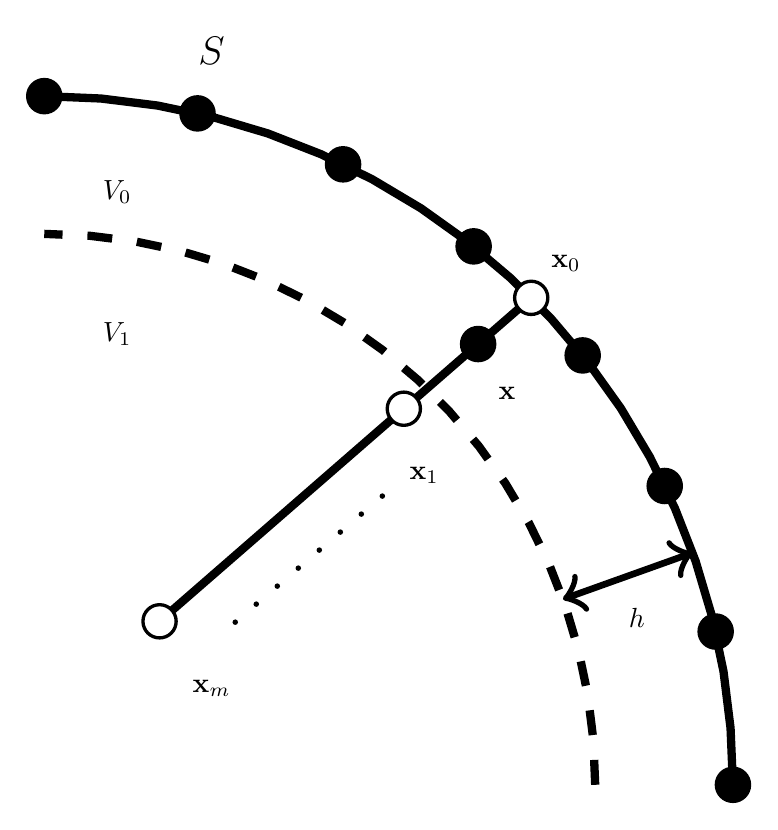
\begin{tikzpicture}[scale=3]

\begin{axis}[
  width=2in, height=2in,
  axis equal,
%  scale only axis,
%  xmin=0, xmax=1.2,
%  ymin=0, ymax=1.2,
  hide axis
  ]
\addplot[color=black,line width =
1.0pt,solid,domain=0:90,samples=20]({cos(\x)},{sin(\x)});
\addplot[color=black,line width =
1.0pt,dashed,domain=0:90,samples=20]({0.8*cos(\x)},{0.8*sin(\x)});
% plot the boundary

\addplot [only marks, mark=*, color=black, fill=black] table{
%1 0
%0.9239 0.3827
%0.7071 0.7071
%0.3827 0.9239
%0 1
1 0
9.7493e-1 2.2252e-1
9.0097e-1 4.3388e-1
7.8183e-1 6.2349e-1
6.2349e-1 7.8183e-1
4.3388e-1 9.0097e-1
2.2252e-1 9.7493e-1
0 1
}; 
% points on the boundary of the geometry 

\addplot [only marks, mark=*,fill=white] coordinates{(0.7071,0.7071)};
\addplot [only marks, mark=*,fill=black] coordinates{(0.6300,0.6400)};
\addplot[color=black,line
width=1.0pt,solid,domain=0:7.2,samples=2]({\x*0.6300+0.7071*(1-\x)},{x*0.6400+0.7071*(1-\x)});
% draw line connecting target point to closest point on boundary
\addplot[only marks, mark=*,fill=white] coordinates {(0.5221,0.5461)};
\addplot[only marks, mark=*,fill=white] coordinates {(0.1674,0.2374)};
% Lagrange interpolation points along 1-d line coming from closest
% point



%\addplot [only marks, mark=*,fill=white] coordinates {(0.6330,0.7742)};
%% open circle which is closest point to curve.  Corresponds to theta =
%% pi/4 + 0.1
%
%%\addplot [color=black,line width = 1.0pt,->,-triangle 60] plot coordinates {(0.6330,0.7742) (1.5*0.6330,1.5*0.7742)};
%% draw the normal vector
%
%\addplot [only marks, mark=*,fill=black] coordinates {(0.5965,0.7004)};
%% plot the target location
%
%
%\addplot[color=black,line
%width=1.0pt,solid,domain=0:10,samples=2]({\x*0.5965+0.6330*(1-\x)},{x*0.7004+0.7742*(1-\x)});
%% draw line connecting target point to closest point on boundary

%\addplot[only marks, mark=*,fill=white] coordinates {(0.2679,0.0369)};
%\addplot[only marks, mark=*,fill=white] coordinates {(0.4869,0.4793)};
% Lagrange interpolation points along 1-d line coming from closest
% point


\addplot [color=black,solid,line width = 0.8pt,<->,name=arrow] plot
coordinates {(0.9415,0.3369) (0.8*0.9415,0.8*0.3369)};
%\addplot [color=black,solid,line width = 0.8pt,->] plot
%coordinates {(0.9808,0.1951) (0.8*0.9808,0.8*0.1951)};
%\addplot [color=black,solid,line width = 0.8pt,<-] plot
%coordinates {(0.9808,0.1951) (0.8*0.9808,0.8*0.1951)};
% width of near zone has an arrow to label its width

\end{axis}

\node[font = \Large] at (1.0,3.4) {$S$};
\node at (2.8,1.0) {$h$};
\node at (2.5,2.5) {$\mathbf{x}_{0}$};
\node at (1.9,1.6) {$\mathbf{x}_{1}$};
\node at (1.0,0.7) {$\mathbf{x}_{m}$};
\node at (2.25,1.95) {$\mathbf{x}$};
\draw[dotted,line cap = round, line width=2pt,dash pattern=on 0pt off
5\pgflinewidth] (1.1,0.98) -- (1.8,1.58);
%\draw[dotted,line cap = round, line width=2pt,dash pattern=on 0pt off
%5\pgflinewidth] (1.1,0.85) -- (1.8,1.45);


%\node at (2.2,2.75) {$\mathbf{x}_{0}$};s
%\node at (2.05,1.55) {$\mathbf{x}_{1}$};
%\node at (1.6,0.3) {$\mathbf{x}_{m}$};
%\node at (1.85,2.35) {$\mathbf{x}$};
%\node[font = \Large] at (0.8,2.85) {$\Omega_{0}$};
%\node[font = \large] at (0.8,2.85) {$\mathtt{Near}(\gamma)$};
%\node[font = \Large] at (0.8,2.0) {$\Omega_{1}$};
%\node[font = \large] at (0.8,2.0) {$\mathtt{Far}(\gamma)$};
%\draw[dotted,line cap = round, line width=2pt,dash pattern=on 0pt off
%5\pgflinewidth] (1.5,0.6) -- (1.9,1.4);

\node at (0.6,2.8) {$V_0$};
\node at (0.6,2.2) {$V_1$};

%\draw[gray,thin] (0,0) grid +(3,4);

\end{tikzpicture}
\end{document}

\caption{Illustration of the near singular integration technique used.}\label{fig:ns_drawing}
\end{center}
\end{figure}

If a target point $\mathbf{x}\in\Omega_1$, we can use the regular trapezoid rule. If $\mathbf{x}\in \Omega_0$, we can find the closest point on the boundary, $\mathbf{x}_0$ using Newton's method. We then add $m$ 
interpolation points
	\[ x_j = x_0 + j\beta h\frac{\mathbf{x}-\mathbf{x}_0}{||\mathbf{x}-\mathbf{x}_0||} \qquad j = 0,\cdots m,\]
where $\beta$ is a constant slightly greater than one to guarantee that all interpolation points are in $\Omega_1$. These points are shown in Figure \ref{fig:ns_drawing}. The layer potential is evaluated at $\mathbf{x}_0$ using a local interpolant of $N_\text{int}$ discretization points on $\Gamma_k$, and also at $\mathbf{x}_j$, $j=1,\cdots,m-1$ using a trapezoid rule with $N^{\sfrac{3}{2}}$ points.  We the use a 1D Lagrange interpolatant to calculate the layer potential at $\mathbf{x}$. When we apply this integration scheme to the double layer potential with a density function in $C^M$, we expect the error to be of $O(h^{\min(N_{\text{int}} - 1, m,  M/2 - 4)})$. In the specific case shown in Figure \ref{fig:near_experiment}, we do not have to iterate to find $\mathbf{x}_0$ since we know that it is at the top of the circle. Taking $m=5$ and noting that $M=\infty$, we expect $O(h^5)$ accuracy, which is demonstrated in Figure \ref{fig:ns_convergence}. 

\begin{figure}[!h]
\begin{center}
% This file was created by matlab2tikz.
%
%The latest updates can be retrieved from
%  http://www.mathworks.com/matlabcentral/fileexchange/22022-matlab2tikz-matlab2tikz
%where you can also make suggestions and rate matlab2tikz.
%
\documentclass[tikz]{standalone}
\usepackage[T1]{fontenc}
\usepackage[utf8]{inputenc}
\usepackage{pgfplots}
\usepackage{grffile}
\pgfplotsset{compat=newest}
\usetikzlibrary{plotmarks}
\usepgfplotslibrary{patchplots}
\usepackage{amsmath}
\usetikzlibrary{decorations.markings}
\definecolor{mycolor1}{rgb}{0.00000,0.44700,0.74100}%
\definecolor{mycolor2}{rgb}{0.85000,0.32500,0.09800}%
\begin{document}

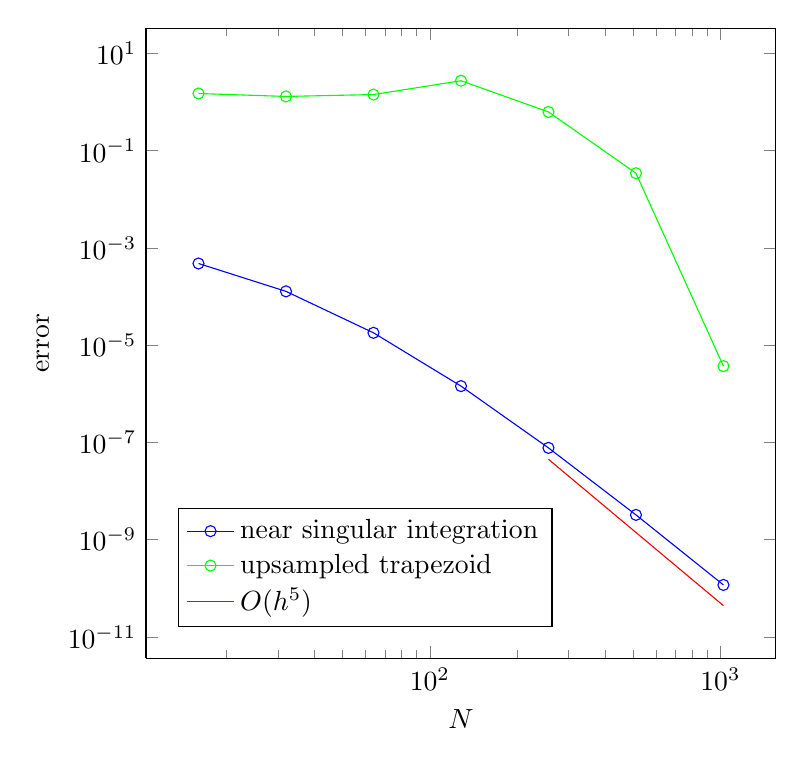
\begin{tikzpicture}

\begin{axis}[%
width=8cm,
height=8cm,
scale only axis,
separate axis lines,
every outer x axis line/.append style={black},
every x tick label/.append style={font=\color{black}},
xmode=log,
xminorticks=true,
xlabel={$N$},
ymode=log,
yminorticks=true,
ylabel={error},
axis background/.style={fill=white},
legend style={legend cell align=left,align=left,draw=black, at={(0.05,0.05)}, anchor=south west}
]
\addplot [color=blue,solid,mark=o,mark options={solid}]
  table[row sep=crcr]{%
16	0.000480141094436615\\
32	0.000128263828182429\\
64	1.80213325182699e-005\\
128	1.44459028306176e-006\\
256	7.75015619458586e-008\\
512	3.2437244001926e-009\\
1024	1.17619469719443e-010\\
};
\addlegendentry{near singular integration};

\addplot [color=green,solid,mark=o,mark options={solid}]
  table[row sep=crcr]{%
16	1.50493118489871\\
32	1.30842630366041\\
64	1.43097492615635\\
128	2.75475486289114\\
256	0.628334046865493\\
512	0.0345181687159036\\
1024	3.7168068580673e-006\\
};
\addlegendentry{upsampled trapezoid};

\addplot [color=red,solid]
  table[row sep=crcr]{%
256	4.51434463456801e-008\\
1024	4.40853968219532e-011\\
};
\addlegendentry{$O(h^5)$};

\end{axis}
\end{tikzpicture}%
\end{document}
\caption[Convergence of the near singular integration scheme.]{Convergence  study for the near singular integration technique with $m=5$ applied to the problem in figure \ref{fig:near_experiment} with $x_2=1.0005$. We see the desired $O(h^5)$ accuracy. The near singular interpolation significantly outperforms even the upsampled trapezoid quadrature for points in $\Omega_0$. }\label{fig:ns_convergence}
\end{center}
\end{figure}




\subsection{Time Stepping}

Once we solve the system \eqref{eq:compact}, we can update the centers $\mathbf{c}_k$ and orientation angle $\theta_k$ of each particle according to
\begin{subequations}
	\begin{align}
		\frac{\text{d} \mathbf{c}_k}{\text{d} t} &= \mathbf{U}_k,\\
		\frac{\text{d}\theta_k}{\text{d} t} &= \omega_k.
	\end{align}
\end{subequations}
This is a system of ordinary differential equations of size $3n$. We compute a solution using the second order two-step explicit Adams-Bashforth method
\[ \mathbf{y}_{n+1} = \mathbf{y}_{n} + \frac{3}{2}\Delta t \mathbf{f}(t_{n}) - \frac{1}{2}\Delta t \mathbf{f}(t_{n-1}).\]

\subsection{Preconditioning}

To precondition the system \eqref{eq:compact}, we note that the velocity contributions in \eqref{eq:compact} can be expressed as a matrix of the form
\begin{equation}\label{eq:matrix}\begin{pmatrix} \mathbf{D}_{pp} & \mathbf{D}_{pw}\\ \mathbf{D}_{wp} & \mathbf{D}_{ww}\end{pmatrix}\begin{pmatrix}\pmb{\eta}_p \\ \pmb{\eta}_w\end{pmatrix}, 
\end{equation}
where $\mathbf{D}_{pp}$ represents the particle-particle interactions, $\mathbf{D}_{ww}$ represents the wall-wall interactions and $\mathbf{D}_{pw}$ and $\mathbf{D}_{wp}$ represent the wall-particle or particle-wall interactions. 

We can write $\mathbf{D}_{pp}$ as
\begin{equation}\label{eq:d_matrix} \begin{pmatrix} \mathbf{D}_{1,1} & \hdots &\mathbf{D}_{1,N} \\ \vdots & \ddots & \vdots \\ \mathbf{D}_{N,1} & \hdots & \mathbf{D}_{N,N}\end{pmatrix},\end{equation}
where $\mathbf{D}_{i,j}$ represents the contribution from points on particle $i$ to points on particle $j$. The other blocks of \eqref{eq:matrix} have similar representations.

The diagonal blocks $\mathbf{D}_{i,i}$ are full rank and so can be inverted directly, while the non diagonal blocks are all low rank. We will use the preconditioner
\[ \begin{pmatrix} \mathbf{D}_{1,1}^{-1} &  & \\ & \ddots \\ & & \mathbf{D}^{-1}_{N,N}\end{pmatrix}.\]
This preconditioner transforms the diagonal blocks into identity matrices. The preconditoned matrix has eigenvalues that are even more clustered than the original, which improves the convergence of GMRES ~\cite{Rasmussen2001}.

\section{Numerical Results}

To test our model, we  run simulations of a Couette apparatus. The inner radius is half the outer radius. The outer wall is stationary and the inner wall has a constant angular velocity. The $N$ particles are parametrized as
\begin{equation}\label{eq:curve}  r(\phi) = (r_x\gamma(\phi,\alpha) \cos(\phi), r_y\gamma(\phi,\alpha)\sin(\phi),\end{equation}
where
\[ \gamma(\phi, \alpha) = (\cos^\alpha(\phi)+\sin^\alpha(\phi))^{\sfrac{1}{\alpha}}.\]
Here $r_x$ is the length of the fiber, $r_y$ is the width, and $\alpha$ is an even natural number that controls the roundedness of the fiber. As can be seen in Figure \ref{fig:curves}, as $\alpha$ increases, the fiber becomes less rounded. For now we will restrict our attention to circular particles, i.e. those with $r_x=r_y$ and $\alpha=2$. 


\begin{figure}[!h]
\begin{center}
\begin{tabular}{c c}
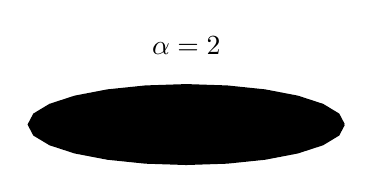
\begin{tikzpicture}
\draw(0, 1) node {$\alpha = 2$};
\draw [thick, fill=black,domain=0:2*pi] plot ({2*(cos(\x r)^2 + sin(\x r)^2)^(-1/2)*cos(\x r)},{ 0.5*(cos(\x r)^2 + sin(\x r)^2)^(-1/4)*sin(\x r) });
\end{tikzpicture}
&
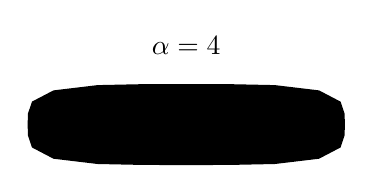
\begin{tikzpicture}
\draw(0, 1) node {$\alpha = 4$};
\draw [thick, fill=black,domain=0:2*pi] plot ({2*(cos(\x r)^4 + sin(\x r)^4)^(-1/4)*cos(\x r)},{ 0.5*(cos(\x r)^4 + sin(\x r)^4)^(-1/4)*sin(\x r) });
\end{tikzpicture}\\
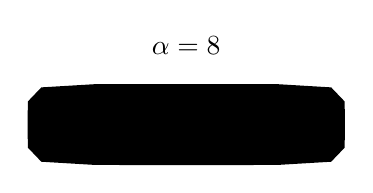
\begin{tikzpicture}
\draw(0, 1) node {$\alpha = 8$};
\draw [thick, fill=black,domain=0:2*pi] plot ({2*(cos(\x r)^8 + sin(\x r)^8)^(-1/8)*cos(\x r)},{ 0.5*(cos(\x r)^8 + sin(\x r)^8)^(-1/8)*sin(\x r) });
\end{tikzpicture}
&
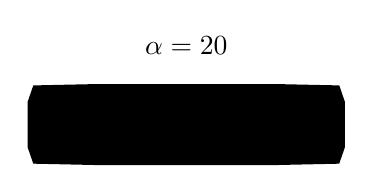
\begin{tikzpicture}
\draw(0, 1) node {$\alpha = 20$};
\draw [thick, fill=black,domain=0:2*pi] plot ({2*(cos(\x r)^20 + sin(\x r)^20)^(-1/20)*cos(\x r)},{ 0.5*(cos(\x r)^20 + sin(\x r)^20)^(-1/20)*sin(\x r) });
\end{tikzpicture}
\end{tabular}
\caption[Effect of the parameter $\alpha$ on the particle parameterization.]{Effect of the parameter $\alpha$ on the shape of the curve given in \eqref{eq:curve}.}\label{fig:curves}
\end{center}
\end{figure}

\begin{figure}[!h]
\begin{center}
% This file was created by matlab2tikz.
%
%The latest updates can be retrieved from
%  http://www.mathworks.com/matlabcentral/fileexchange/22022-matlab2tikz-matlab2tikz
%where you can also make suggestions and rate matlab2tikz.
%
\definecolor{mycolor1}{rgb}{0.00000,0.44700,0.74100}%
%
\begin{tikzpicture}

\begin{axis}[%
width=11.411cm,
height=2.647cm,
at={(0cm,7.353cm)},
scale only axis,
xmin=-10,
xmax=70,
ymin=-0.5,
ymax=0.5,
axis background/.style={fill=white}
]
\addplot [color=mycolor1, draw=none, mark=*, mark options={solid, mycolor1}, forget plot]
  table[row sep=crcr]{%
62.831853071796	0\\
-9.63809516230732	0\\
-5.65438740619943	0\\
-5.65454747914734	0\\
3.13221442414912	0\\
-1.75173194132456	0\\
-1.75106886806812	0\\
1.3121131926913	0\\
1.31213262347105	0\\
1.31220873880399	0\\
1.31220177591532	0\\
-1.31204866939091	0\\
-1.31197680952783	0\\
-1.31178190662804	0\\
-1.31182739558626	0\\
-1.00229283239403	0\\
0.00444841132607919	0.349570127838051\\
0.00444841132607919	-0.349570127838051\\
0.00444650181683529	0.349577426551913\\
0.00444650181683529	-0.349577426551913\\
0.027648531919956	0\\
0.0275408203251815	0\\
-1.00001473938421	0\\
-1.00230208283965	0\\
-0.913475188045221	0\\
-0.913203603509879	0\\
-0.783264961162645	0\\
-0.797690234639255	0\\
-0.795072958788542	0\\
-0.0867633387531751	0\\
-0.086454908420536	0\\
-0.704618672014923	0\\
-0.201065910006729	0\\
-0.204906958812501	0\\
-0.256125682361871	0\\
-0.262295596982938	0\\
-0.29991810955159	0\\
-0.299298589118389	0\\
-0.295344161846994	0\\
-0.295628502076724	0\\
-0.309442719206459	0\\
-0.307386937649929	0\\
-0.692966052623058	0\\
-0.673947348666803	0\\
-0.65700525517248	0\\
-0.634797508412241	0\\
-0.628636018306197	0\\
-0.619588636334102	0\\
-0.612757443333672	0\\
-0.366447056407823	0\\
-0.374055750575542	0.00172145108519279\\
-0.374055750575542	-0.00172145108519279\\
-0.380827576966074	0\\
-0.606927793857927	0\\
-0.606561131528505	0\\
-0.59001863734667	0\\
-0.597591247831646	0\\
-0.598530205258242	0\\
-0.395601272452172	0\\
-0.401413443800875	0\\
-0.409193441362996	0\\
-0.40989016214058	0\\
-0.585732267929368	0\\
-0.570323223549959	0\\
-0.563732584605295	0\\
-0.427325255313001	0\\
-0.430339038332032	0\\
-0.429046422174476	0\\
-0.438054683252914	0\\
-0.540697547856837	0\\
-0.539832049955014	0\\
-0.537354219241891	6.91260987850949e-05\\
-0.537354219241891	-6.91260987850949e-05\\
-0.459704902381227	0\\
-0.461642857743143	0\\
-0.462879461896028	0\\
-0.464439557040398	0\\
-0.531543730494462	0\\
-0.529801117281715	0\\
-0.477064092876016	0\\
-0.477444212708187	0\\
-0.526226573370666	0\\
-0.523142085636774	0\\
-0.520199709630084	0\\
-0.518845620527375	0\\
-0.519672306530397	0\\
-0.485754942669686	0\\
-0.486482294310137	0\\
-0.486875257276835	0\\
-0.487649932320891	0\\
-0.513990777884687	0\\
-0.513866099920225	0\\
-0.513216374251318	0\\
-0.512570523309505	0\\
-0.511794809385919	0\\
-0.510007746386277	0\\
-0.491080045352677	0\\
-0.508073329559867	0\\
-0.506755221191686	0\\
-0.492954464306218	0\\
-0.505542701682797	0\\
-0.493721712907177	0\\
-0.494191556744449	0\\
-0.494867715320814	0\\
-0.504273370564503	0\\
-0.504105274366122	0\\
-0.503581241303304	0\\
-0.4957512737237	0\\
-0.496704818603197	0\\
-0.496642543857489	0\\
-0.502688367500095	0\\
-0.497433889434443	0\\
-0.497697140243399	0\\
-0.501885267091932	0\\
-0.501812422211208	0\\
-0.501710594484467	0\\
-0.49828334492139	0\\
-0.498309279324649	0\\
-0.501363208983448	0\\
-0.498581713628181	0\\
-0.498847608357006	0\\
-0.500962664569223	0\\
-0.500792136490365	0\\
-0.500747055002026	0\\
-0.500665231255126	0\\
-0.499138065175112	0\\
-0.499225679417616	0\\
-0.499300671890372	0\\
-0.499374311575271	0\\
-0.500484171584179	0\\
-0.499597750458702	0\\
-0.499653141830794	3.2990691706111e-06\\
-0.499653141830794	-3.2990691706111e-06\\
-0.49967629034478	0\\
-0.500360108361687	0\\
-0.500343271448191	0\\
-0.500320361604168	0\\
-0.500231886510867	0\\
-0.499822895478226	8.26015308672626e-06\\
-0.499822895478226	-8.26015308672626e-06\\
-0.499829349915457	0\\
-0.49984149188501	0\\
-0.500175463314922	0\\
-0.500163942200935	0\\
-0.500139171269537	0\\
-0.500112360245517	0\\
-0.500092841646465	0\\
-0.500084258616321	0\\
-0.499914161282769	0\\
-0.499918641072986	6.5507104948668e-06\\
-0.499918641072986	-6.5507104948668e-06\\
-0.499927278003784	0\\
-0.50005694328297	2.12276094417099e-05\\
-0.50005694328297	-2.12276094417099e-05\\
-0.500060889506629	0\\
-0.500056498882723	0\\
-0.50003274521493	1.78388215453713e-05\\
-0.50003274521493	-1.78388215453713e-05\\
-0.500035631016886	5.1458421247954e-07\\
-0.500035631016886	-5.1458421247954e-07\\
-0.499957305762835	0\\
-0.499961951204651	1.39716418824181e-06\\
-0.499961951204651	-1.39716418824181e-06\\
-0.49996592711915	0\\
-0.50002033880006	9.5353589685713e-06\\
-0.50002033880006	-9.5353589685713e-06\\
-0.500018187972646	0\\
-0.500017762377125	0\\
-0.499979323229261	0\\
-0.499981613067205	0\\
-0.499983030890605	0\\
-0.499984719756665	0\\
-0.500010486550263	3.36082780575485e-06\\
-0.500010486550263	-3.36082780575485e-06\\
-0.500008942157629	0\\
-0.500008142821189	0\\
-0.499990629900033	0\\
-0.499991461490606	5.46294352202526e-07\\
-0.499991461490606	-5.46294352202526e-07\\
-0.499993138585016	0\\
-0.500004745852357	1.46091256933457e-06\\
-0.500004745852357	-1.46091256933457e-06\\
-0.500004277963318	0\\
-0.500003628477555	0\\
-0.49999588879344	4.73249779881602e-07\\
-0.49999588879344	-4.73249779881602e-07\\
-0.499996046356267	0\\
-0.49999706695858	0\\
-0.500001684509396	9.52622810416293e-07\\
-0.500001684509396	-9.52622810416293e-07\\
-0.500002024329123	0\\
-0.499998149344434	3.65186528937089e-07\\
-0.499998149344434	-3.65186528937089e-07\\
-0.499998288567745	0\\
-0.50000175014206	0\\
-0.500001185916982	8.10179431492198e-07\\
-0.500001185916982	-8.10179431492198e-07\\
-0.499998768443593	0\\
-0.500000036255833	8.38751041434497e-07\\
-0.500000036255833	-8.38751041434497e-07\\
-0.500000927062184	0\\
-0.500000795984198	0\\
-0.499999233072753	1.41000243894183e-07\\
-0.499999233072753	-1.41000243894183e-07\\
-0.500000572166805	0\\
-0.499999315120246	0\\
-0.499999599760505	0\\
-0.500000359457923	0\\
-0.499999730583618	0\\
-0.499999750195203	0\\
-0.499999782869115	1.18805764136426e-08\\
-0.499999782869115	-1.18805764136426e-08\\
-0.500000242963735	0\\
-0.50000022518227	0\\
-0.500000217811936	0\\
-0.499999890429657	0\\
-0.499999903387992	2.84118092425822e-10\\
-0.499999903387992	-2.84118092425822e-10\\
-0.499999915303822	0\\
-0.500000120580459	0\\
-0.500000090751208	8.4985098492128e-09\\
-0.500000090751208	-8.4985098492128e-09\\
-0.500000084497272	0\\
-0.500000041714261	0\\
-0.500000066590395	0\\
-0.499999968693594	0\\
-0.499999976421164	0\\
-0.499999997045162	0\\
-0.499999998882349	0\\
-0.499999999956057	0\\
-0.500000000056302	0\\
-0.500000000009106	0\\
-0.50000000001622	0\\
};
\node[right, align=left]
at (axis cs:30,0.35) {Unknowns = 233};
\node[right, align=left]
at (axis cs:30,0.2) {Cond = 5564};
\node[right, align=left]
at (axis cs:30,0.05) {Iterations = 19};
\end{axis}

\begin{axis}[%
width=11.411cm,
height=2.647cm,
at={(0cm,3.676cm)},
scale only axis,
xmin=-10,
xmax=70,
ymin=-0.5,
ymax=0.5,
axis background/.style={fill=white}
]
\addplot [color=mycolor1, draw=none, mark=*, mark options={solid, mycolor1}, forget plot]
  table[row sep=crcr]{%
62.8318530717958	0\\
-9.63809823397995	0\\
-5.65454892640938	0\\
-5.65438951842999	0\\
3.13218113215365	0\\
1.32372599201956	0\\
1.32372625433686	0\\
1.32372736324311	0\\
1.32372723887864	0\\
-1.75105332182908	0\\
-1.75167366775738	0\\
-1.32374175578257	0\\
-1.3237388034637	0\\
-1.32373848107741	0\\
-1.32374060986588	0\\
4.11738578324078e-05	0.360689253171236\\
4.11738578324078e-05	-0.360689253171236\\
4.11859790344776e-05	0.360689205263978\\
4.11859790344776e-05	-0.360689205263978\\
0.0276516894751897	0\\
0.0275364354223012	0\\
-0.999999999778507	0\\
-1.00000953076243	0\\
-1.00000954080663	0\\
-0.91324916210433	0\\
-0.913483644956195	0\\
-0.0865178349707992	0\\
-0.0867468119989938	0\\
-0.795105409002859	0\\
-0.797765586162695	0\\
-0.783334521982829	0\\
-0.20222692725353	0\\
-0.204891193104331	0\\
-0.708783660969335	0\\
-0.693681060336513	0\\
-0.692955143784693	0\\
-0.288546693636197	0\\
-0.676804268144685	0\\
-0.65504344881217	0\\
-0.6534425178151	0\\
-0.646279659721784	0\\
-0.645966528254168	0\\
-0.627156558719566	0\\
-0.30455066503429	0\\
-0.306987693876052	0\\
-0.32072228654888	0\\
-0.341524755652575	0\\
-0.343319588691472	0\\
-0.350219713737765	0\\
-0.350519050904608	0\\
-0.365738304445979	0\\
-0.375774036136985	0.000410556409660548\\
-0.375774036136985	-0.000410556409660548\\
-0.380978921538751	0\\
-0.618988933696447	0\\
-0.609919553401616	0\\
-0.60617249905573	0\\
-0.388201744747695	0\\
-0.401608343958776	0\\
-0.402986019548445	0\\
-0.410617006256611	0\\
-0.595059909925189	0\\
-0.588710715567567	0\\
-0.570405377735601	0\\
-0.429563202061285	0\\
-0.563930919349854	0\\
-0.43582459048497	0\\
-0.450647930833874	0\\
-0.45069860996449	0\\
-0.459658835970913	0\\
-0.459391203956994	0\\
-0.461984521828703	0\\
-0.462769890852222	0\\
-0.54243524485738	0\\
-0.542424136249146	0\\
-0.540757300248509	0\\
-0.540365597174627	0\\
-0.537768001469633	0\\
-0.537196177145943	0\\
-0.532966943953027	0\\
-0.470992156979034	0\\
-0.471218195953851	0\\
-0.530037388538751	0\\
-0.473518599668593	0\\
-0.475662519991773	0\\
-0.477565896458504	0\\
-0.527677193126184	0\\
-0.52513616898974	0\\
-0.522257586242797	0\\
-0.521523751212709	0\\
-0.520757356189319	0\\
-0.480852954166073	0\\
-0.481139784467408	0\\
-0.48162935390917	0\\
-0.517713747787643	0\\
-0.517572498052533	0\\
-0.516074614152856	0\\
-0.513039331349275	0\\
-0.513261557504716	0\\
-0.486742124165657	2.6992258481573e-06\\
-0.486742124165657	-2.6992258481573e-06\\
-0.487339410248664	0\\
-0.487525474941945	0\\
-0.487659813209394	0\\
-0.488957858701666	0\\
-0.510823732642565	0\\
-0.510249339337734	0\\
-0.490641440132961	0\\
-0.492673453489136	0\\
-0.507936765657329	0\\
-0.507874382206764	0\\
-0.49320191879746	0\\
-0.493516769084543	0\\
-0.507349760529317	0\\
-0.494051809051679	0\\
-0.494324026068373	0\\
-0.506792700887381	0\\
-0.506568991648006	0\\
-0.506449601620482	0\\
-0.505791896361143	0.000149055220368286\\
-0.505791896361143	-0.000149055220368286\\
-0.505945749475329	0\\
-0.505295564373159	0\\
-0.504406724172014	0\\
-0.504053137287377	0\\
-0.495724984395807	0\\
-0.495782044550084	0\\
-0.503550943223896	0\\
-0.496166610659976	0\\
-0.496431799239243	0\\
-0.496531782153837	0\\
-0.502962348335642	0\\
-0.497092747170991	0\\
-0.502080978867168	0\\
-0.498082784931098	0\\
-0.498105884027992	0\\
-0.498168552762611	0\\
-0.501961856927805	0\\
-0.501911532569296	0\\
-0.501883422147865	0\\
-0.498347735029495	0\\
-0.501732664335453	0\\
-0.501681989662646	0\\
-0.501440274368707	0\\
-0.50142802362633	0\\
-0.49861588417198	0\\
-0.498631942997457	0\\
-0.49889419053516	0\\
-0.498905246934668	0\\
-0.501004247063436	0\\
-0.500983137899828	0\\
-0.49903230040759	0\\
-0.50090590418064	0\\
-0.499184649073612	0\\
-0.499207259588967	0\\
-0.499269014282408	0\\
-0.500804643879811	0\\
-0.500713152473765	0\\
-0.500673607210853	0\\
-0.50058548038237	0\\
-0.500512215139997	0\\
-0.500475778729083	0\\
-0.499504430979197	0\\
-0.49951948496058	0\\
-0.499610847733399	0\\
-0.499649880695489	0\\
-0.50036599567339	0\\
-0.500328937732785	0\\
-0.500320015402419	0\\
-0.49971269584217	0\\
-0.500239412289733	0\\
-0.499760948635334	0\\
-0.499777331891876	0\\
-0.500187877243982	0\\
-0.500178018310199	0\\
-0.500161839829507	0\\
-0.499833008723609	0\\
-0.499843326768287	0\\
-0.499867645935227	0\\
-0.499886075418278	0\\
-0.500121814395804	0\\
-0.500106358296037	0\\
-0.500092253688295	0\\
-0.499909105757657	0\\
-0.500080361014131	0\\
-0.499924029408397	0\\
-0.499926484399348	0\\
-0.500069969418923	0\\
-0.500061339999857	0\\
-0.499943452561384	0\\
-0.499949004376782	0\\
-0.500043495755891	0\\
-0.500041165746874	0\\
-0.500038355493556	0\\
-0.499958513624665	0\\
-0.499963064884393	0\\
-0.500033615552004	0\\
-0.499969483438539	0\\
-0.499971607339068	0\\
-0.499978135556753	0\\
-0.499980753740694	0\\
-0.500021333777609	0\\
-0.500020150252528	0\\
-0.500019577891211	0\\
-0.500017835676504	0\\
-0.499983458533547	0\\
-0.499984863943575	0\\
-0.500011549333708	0\\
-0.499988428197449	0\\
-0.499989292937564	0\\
-0.500009303472702	7.74371912028768e-08\\
-0.500009303472702	-7.74371912028768e-08\\
-0.500008886051844	0\\
-0.49999165056201	0\\
-0.499991901100408	0\\
-0.500006729187495	0\\
-0.499993453317074	0\\
-0.499994047596835	0\\
-0.500004759684825	0\\
-0.500004429330706	0\\
-0.500004360595544	0\\
-0.500003961441183	0\\
-0.49999574122422	0\\
-0.499995939801139	0\\
-0.49999631282531	0\\
-0.499996995250811	0\\
-0.500002946857637	0\\
-0.500002340794998	0\\
-0.499997903239568	0\\
-0.499997962589293	0\\
-0.499998059835857	0\\
-0.500001978870999	0\\
-0.500001849656182	0\\
-0.500001792239926	0\\
-0.499998511008941	0\\
-0.50000117201926	0\\
-0.499998937836372	0\\
-0.49999896928986	0\\
-0.499999026316704	0\\
-0.500000984185813	0\\
-0.500000920807415	0\\
-0.500000856210316	0\\
-0.499999278041761	0\\
-0.500000585470753	0\\
-0.500000513408008	0\\
-0.49999945873488	0\\
-0.499999474947625	0\\
-0.499999511083122	0\\
-0.500000433508777	0\\
-0.500000392024356	0\\
-0.499999647155542	0\\
-0.500000289603477	0\\
-0.500000258042835	0\\
-0.499999717534788	0\\
-0.49999972622188	0\\
-0.499999750615193	0\\
-0.500000207496972	0\\
-0.500000183197722	0\\
-0.499999828695753	0\\
-0.499999842954613	0\\
-0.50000013940864	0\\
-0.500000128671252	0\\
-0.499999864782859	0\\
-0.499999871772812	0\\
-0.50000010063068	0\\
-0.500000087505028	0\\
-0.499999914992662	1.20895756562449e-09\\
-0.499999914992662	-1.20895756562449e-09\\
-0.500000063186703	2.83785843058489e-09\\
-0.500000063186703	-2.83785843058489e-09\\
-0.499999933856875	0\\
-0.499999937156123	0\\
-0.500000049307843	0\\
-0.500000042804554	0\\
-0.499999956172784	0\\
-0.49999995834687	0\\
-0.49999996806142	0\\
-0.500000028947892	1.79028074067956e-09\\
-0.500000028947892	-1.79028074067956e-09\\
-0.499999971714886	0\\
-0.499999975915669	0\\
-0.50000002439072	0\\
-0.500000021211205	0\\
-0.499999979757068	0\\
-0.499999984700048	0\\
-0.499999995518912	1.09169964875829e-08\\
-0.499999995518912	-1.09169964875829e-08\\
-0.500000013847855	0\\
-0.499999988668249	1.62186492502421e-09\\
-0.499999988668249	-1.62186492502421e-09\\
-0.500000012202811	0\\
-0.500000011803334	0\\
-0.50000001037434	0\\
-0.499999990212843	0\\
-0.499999992678402	0\\
-0.500000006712335	0\\
-0.499999999384323	5.43020305651004e-09\\
-0.499999999384323	-5.43020305651004e-09\\
-0.50000000607765	0\\
-0.500000005233074	0\\
-0.499999995017867	7.04515193708686e-10\\
-0.499999995017867	-7.04515193708686e-10\\
-0.500000004416495	0\\
-0.499999995654371	0\\
-0.499999996445736	0\\
-0.500000003105472	6.69417776304947e-11\\
-0.500000003105472	-6.69417776304947e-11\\
-0.500000002532657	0\\
-0.499999997464235	1.26565084245141e-10\\
-0.499999997464235	-1.26565084245141e-10\\
-0.500000001926302	0\\
-0.4999999983537	1.51580022227796e-10\\
-0.4999999983537	-1.51580022227796e-10\\
-0.500000001497785	9.1154798902692e-11\\
-0.500000001497785	-9.1154798902692e-11\\
-0.500000001233508	0\\
-0.499999998759238	7.0583119749159e-11\\
-0.499999998759238	-7.0583119749159e-11\\
-0.500000000877937	0\\
-0.500000000703668	5.45280864125169e-11\\
-0.500000000703668	-5.45280864125169e-11\\
-0.499999999266469	7.20967421359076e-11\\
-0.499999999266469	-7.20967421359076e-11\\
-0.500000000591916	0\\
-0.499999999372193	0\\
-0.499999999403745	0\\
-0.500000000427807	0\\
-0.500000000331446	2.43168099707011e-11\\
-0.500000000331446	-2.43168099707011e-11\\
-0.500000000286963	0\\
-0.499999999672579	2.67689830052935e-11\\
-0.499999999672579	-2.67689830052935e-11\\
-0.499999999705023	1.1246791793016e-11\\
-0.499999999705023	-1.1246791793016e-11\\
-0.500000000205994	0\\
-0.49999999984261	0\\
-0.500000000153985	0\\
-0.500000000143184	7.47666413457141e-12\\
-0.500000000143184	-7.47666413457141e-12\\
-0.499999999859237	8.998008785434e-12\\
-0.499999999859237	-8.998008785434e-12\\
-0.499999999866175	0\\
-0.500000000100493	0\\
-0.499999999950003	6.25214916939909e-11\\
-0.499999999950003	-6.25214916939909e-11\\
-0.500000000076417	0\\
-0.500000000064244	5.03033023185648e-12\\
-0.500000000064244	-5.03033023185648e-12\\
-0.499999999928221	0\\
-0.499999999932404	0\\
-0.499999999936044	0\\
-0.500000000048213	0\\
-0.499999999952081	0\\
-0.500000000035289	0\\
-0.499999999967622	0\\
-0.499999999967966	0\\
-0.500000000028873	2.95254091116784e-12\\
-0.500000000028873	-2.95254091116784e-12\\
-0.499999999970214	0\\
-0.500000000022493	0\\
-0.499999999979582	0\\
-0.500000000016223	0\\
-0.499999999985545	5.89415614806563e-13\\
-0.499999999985545	-5.89415614806563e-13\\
-0.499999999986169	0\\
-0.500000000012905	7.13811323854449e-13\\
-0.500000000012905	-7.13811323854449e-13\\
-0.499999999991304	0\\
-0.500000000010382	0\\
-0.500000000003655	7.46494828039109e-12\\
-0.500000000003655	-7.46494828039109e-12\\
-0.50000000000682	0\\
-0.499999999993333	0\\
-0.499999999993907	2.80051836198692e-13\\
-0.499999999993907	-2.80051836198692e-13\\
-0.500000000005774	6.31852588765548e-13\\
-0.500000000005774	-6.31852588765548e-13\\
-0.500000000004252	0\\
-0.499999999996152	0\\
-0.499999999996945	0\\
-0.499999999997243	1.03992219302052e-13\\
-0.499999999997243	-1.03992219302052e-13\\
-0.500000000003108	0\\
-0.500000000002722	0\\
-0.500000000002324	0\\
-0.499999999998296	0\\
-0.500000000001659	0\\
-0.500000000001378	0\\
-0.50000000000118	0\\
-0.499999999998596	0\\
-0.499999999998835	0\\
-0.499999999999109	1.09041140898633e-13\\
-0.499999999999109	-1.09041140898633e-13\\
-0.500000000000775	1.52700923474596e-13\\
-0.500000000000775	-1.52700923474596e-13\\
-0.500000000000457	4.55397086997922e-13\\
-0.500000000000457	-4.55397086997922e-13\\
-0.500000000000564	1.07958414591972e-13\\
-0.500000000000564	-1.07958414591972e-13\\
-0.499999999999417	0\\
-0.499999999999496	0\\
-0.499999999999571	4.43106290280034e-14\\
-0.499999999999571	-4.43106290280034e-14\\
-0.500000000000355	1.23361278713249e-13\\
-0.500000000000355	-1.23361278713249e-13\\
-0.499999999999789	1.87889052050986e-14\\
-0.499999999999789	-1.87889052050986e-14\\
-0.499999999999799	0\\
-0.499999999999852	0\\
-0.500000000000207	6.5360084506955e-14\\
-0.500000000000207	-6.5360084506955e-14\\
-0.500000000000166	9.37679473244436e-14\\
-0.500000000000166	-9.37679473244436e-14\\
-0.4999999999999	0\\
-0.499999999999946	6.29117710125981e-14\\
-0.499999999999946	-6.29117710125981e-14\\
-0.49999999999995	0\\
-0.500000000000073	0\\
-0.500000000000055	2.05558100321729e-14\\
-0.500000000000055	-2.05558100321729e-14\\
-0.499999999999978	1.28267701380035e-14\\
-0.499999999999978	-1.28267701380035e-14\\
-0.499999999999986	1.63267912261641e-14\\
-0.499999999999986	-1.63267912261641e-14\\
-0.500000000000026	0\\
-0.499999999999979	0\\
-0.499999999999985	0\\
-0.499999999999992	8.77866340433944e-15\\
-0.499999999999992	-8.77866340433944e-15\\
-0.500000000000024	0\\
-0.500000000000004	1.07392469859256e-14\\
-0.500000000000004	-1.07392469859256e-14\\
-0.500000000000021	0\\
-0.500000000000014	0\\
-0.499999999999992	2.83103469840401e-15\\
-0.499999999999992	-2.83103469840401e-15\\
-0.500000000000011	2.74317215622895e-15\\
-0.500000000000011	-2.74317215622895e-15\\
-0.499999999999993	1.47183083316214e-15\\
-0.499999999999993	-1.47183083316214e-15\\
-0.500000000000005	2.62660965578179e-15\\
-0.500000000000005	-2.62660965578179e-15\\
-0.500000000000009	0\\
-0.500000000000008	0\\
-0.499999999999999	0\\
-0.499999999999997	0\\
-0.499999999999999	7.04357546757435e-16\\
-0.499999999999999	-7.04357546757435e-16\\
-0.500000000000003	0\\
-0.500000000000001	0\\
-0.5	3.9055556787155e-16\\
-0.5	-3.9055556787155e-16\\
-0.500000000000001	0\\
-0.499999999999999	0\\
-0.500000000000001	0\\
-0.5	0\\
-0.5	0\\
};
\node[right, align=left]
at (axis cs:30,0.35) {Unknowns = 457};
\node[right, align=left]
at (axis cs:30,0.2) {Cond = 5229};
\node[right, align=left]
at (axis cs:30,0.05) {Iterations = 18};
\end{axis}

\begin{axis}[%
width=11.411cm,
height=2.647cm,
at={(0cm,0cm)},
scale only axis,
xmin=-10,
xmax=70,
ymin=-0.5,
ymax=0.5,
axis background/.style={fill=white}
]
\addplot [color=mycolor1, draw=none, mark=*, mark options={solid, mycolor1}, forget plot]
  table[row sep=crcr]{%
62.831853071796	0\\
-9.63809837628691	0\\
-5.6545492468893	0\\
-5.6543895263252	0\\
3.1321691846537	0\\
-1.7510471608954	0\\
-1.75167225858372	0\\
1.32454185607189	0\\
1.32454185614392	0\\
1.32454185627949	0\\
1.32454185625524	0\\
-1.32454187319943	0\\
-1.32454187375202	0\\
-1.32454187409162	0\\
-1.32454187392822	0\\
-4.40193671930045e-08	0.36118314965864\\
-4.40193671930045e-08	-0.36118314965864\\
-4.40021300238472e-08	0.361183149538104\\
-4.40021300238472e-08	-0.361183149538104\\
0.0276538331461748	0\\
0.027529117442059	0\\
-0.0865476069498922	0\\
-0.0867205680021719	0\\
-0.913275331548474	0\\
-0.91345457363967	0\\
-1.00000001981265	0\\
-1.00000001885758	0\\
-0.999999999999999	0\\
-0.202467010798301	0\\
-0.204819029948276	0\\
-0.797550588135828	0\\
-0.795177335817822	0\\
-0.783081918412607	0\\
-0.707748222153546	0\\
-0.695014147156057	0\\
-0.691576649775515	0\\
-0.29063715230786	0\\
-0.681436454363452	0\\
-0.304271839439717	0\\
-0.308124223986419	0\\
-0.317961345287673	0\\
-0.656596087211862	0\\
-0.65516108859842	0\\
-0.648159712880902	0\\
-0.647958459665029	0\\
-0.629593108057598	0\\
-0.342874115776493	0\\
-0.344575442619867	0\\
-0.352029264543853	0\\
-0.351824902047761	0\\
-0.619080312709316	0\\
-0.367230143837861	0\\
-0.374372241149086	0.00138393756338992\\
-0.374372241149086	-0.00138393756338992\\
-0.380921587480628	0\\
-0.610978196597956	0\\
-0.604406436929058	0\\
-0.39015997609431	0\\
-0.594723655088489	0\\
-0.590270776436951	0\\
-0.398967894669204	0\\
-0.406548984365436	0\\
-0.410426409062344	0\\
-0.570360157886457	0\\
-0.429619001475135	0\\
-0.564210169708079	0\\
-0.435644973030371	0\\
-0.454550721738127	0\\
-0.454569470012076	0\\
-0.545416813391347	0\\
-0.545401431108713	0\\
-0.459191226079627	0\\
-0.459462484953448	0\\
-0.462375500464349	0\\
-0.46267533534081	0\\
-0.540888973612726	0\\
-0.540709480413956	0\\
-0.53733705797718	0\\
-0.537641646549502	0\\
-0.533076888780762	0\\
-0.53058206379091	0\\
-0.470403771520192	0\\
-0.528684105792425	0\\
-0.473688998404789	0\\
-0.473950289522934	0\\
-0.525449858665475	0\\
-0.476593474423773	0\\
-0.47799610090713	0\\
-0.522277946140245	0\\
-0.522221677758906	0\\
-0.521860538555518	0\\
-0.480960911085562	0\\
-0.481188164353295	0\\
-0.519012000176098	0\\
-0.518804165716336	0\\
-0.517163258778976	0\\
-0.482746779676334	0\\
-0.513267514709056	0\\
-0.513170064803681	0\\
-0.486732085309972	0\\
-0.48682773017066	0\\
-0.511410490296472	0\\
-0.488404242252955	0\\
-0.510801087065924	0\\
-0.489040470076418	0\\
-0.509406626852403	0\\
-0.509220203756057	0\\
-0.49052998914744	0\\
-0.49072199484511	0\\
-0.507719032209674	0\\
-0.492191607346744	0\\
-0.50737934665969	0\\
-0.492568887560936	0\\
-0.493184008001155	0\\
-0.493260820370259	0\\
-0.493497652924602	0\\
-0.506785594192689	0\\
-0.506620228111221	0\\
-0.50636214483707	0\\
-0.505595790323902	0\\
-0.494397489287515	0\\
-0.494759604295966	0\\
-0.494880424653439	0\\
-0.505222233855687	0\\
-0.505083213387013	0\\
-0.495639511817696	0\\
-0.495814426734886	0\\
-0.504349747993776	0\\
-0.504164066865312	0\\
-0.496479870666169	0\\
-0.503500518468483	0\\
-0.496919557885136	0\\
-0.503030889764411	0\\
-0.497687909908368	0\\
-0.497688256499335	0\\
-0.502260084149098	0\\
-0.502259934832601	0\\
-0.498041633846203	0\\
-0.498149049515406	0\\
-0.49810087413914	0\\
-0.498298979288424	0\\
-0.501955357211063	0\\
-0.501896636753914	0\\
-0.501846188729362	0\\
-0.501693598895223	0\\
-0.498689705340574	0\\
-0.501292084349042	0\\
-0.498845769675213	0\\
-0.501145809497469	0\\
-0.498991173164945	0\\
-0.501004046677513	0\\
-0.499102285608961	0\\
-0.499169672713858	0\\
-0.500891927926989	0\\
-0.499234624648422	0\\
-0.500827174196964	0\\
-0.50076296794143	0\\
-0.500605478589226	0\\
-0.500592684375251	0\\
-0.49938693446282	0\\
-0.499402256891881	0\\
-0.499423561142593	0\\
-0.500554944901342	0\\
-0.499458849493039	0\\
-0.500520335116006	0\\
-0.499510198187518	0\\
-0.499528396341679	0\\
-0.500478087054043	0\\
-0.49955046732636	0\\
-0.500454824164203	0\\
-0.499592524546573	0\\
-0.500430157628794	0\\
-0.499614279517382	0\\
-0.499645035457171	0\\
-0.499670071765598	0\\
-0.499681242382477	0\\
-0.500391240008946	0\\
-0.500376747182594	0\\
-0.500353711625011	0\\
-0.500327685755938	0\\
-0.500312881752656	0\\
-0.500236834426059	0\\
-0.499762539191281	0\\
-0.500226906222312	0\\
-0.499773759509463	0\\
-0.500203777471026	0\\
-0.500197943294079	0\\
-0.499796933447468	0\\
-0.499801577960622	0\\
-0.500174388509116	0\\
-0.499826212146233	0\\
-0.50015900256983	0\\
-0.499841013375015	0\\
-0.50015110375617	0\\
-0.499850842618303	0\\
-0.500138754612133	0\\
-0.500132217547514	0\\
-0.499864796313616	0\\
-0.500123902568994	0\\
-0.499870563224964	0\\
-0.499878323198589	0\\
-0.500105997876588	0\\
-0.499894079524027	0\\
-0.500097251708475	0\\
-0.499903367935791	0\\
-0.49990872782126	0\\
-0.499908975780715	0\\
-0.499920802410789	0\\
-0.499922675486848	0\\
-0.500084874096236	0\\
-0.500084929679782	0\\
-0.500078980209763	0\\
-0.500077894213012	0\\
-0.500051781827502	0\\
-0.500051123166457	0\\
-0.499947976205312	0\\
-0.499949195474673	0\\
-0.499956398751868	0\\
-0.499957583868315	0\\
-0.500043989514667	0\\
-0.500042726419173	0\\
-0.500035231274648	0\\
-0.500030696029184	0\\
-0.500029877986658	0\\
-0.499967209574853	0\\
-0.500027559428083	0\\
-0.499969627758742	0\\
-0.499970034386227	0\\
-0.500025519644274	0\\
-0.4999715541333	0\\
-0.499973298974881	0\\
-0.499975137563689	0\\
-0.499976293128153	0\\
-0.50002275149091	0\\
-0.499978135319054	0\\
-0.500021787199835	0\\
-0.500019988039447	0\\
-0.499980159812613	0\\
-0.499980272257925	0\\
-0.499981029716197	0\\
-0.50001782689794	0\\
-0.500017206194936	0\\
-0.499983379009577	0\\
-0.500015646920859	0\\
-0.500013910339228	0\\
-0.499984619419426	0\\
-0.499985462276735	0\\
-0.499984923147919	0\\
-0.499986671235355	0\\
-0.500013625259558	0\\
-0.500013372528626	0\\
-0.500012967678641	0\\
-0.499987826807147	0\\
-0.500012088184206	0\\
-0.500011632765558	0\\
-0.499989053801588	0\\
-0.499990600310319	0\\
-0.50001073199632	0\\
-0.500009806460353	0\\
-0.500009539630508	0\\
-0.499991438852863	0\\
-0.499991902519327	0\\
-0.500008951401146	0\\
-0.500008757262575	0\\
-0.500008264081564	0\\
-0.500007652141813	0\\
-0.499992443205771	0\\
-0.499992709772823	0\\
-0.499993018580886	0\\
-0.500006878686465	0\\
-0.499994138059494	0\\
-0.500005812381278	0\\
-0.49999461361889	0\\
-0.500004783155498	0\\
-0.500004507774375	0\\
-0.500004304818969	0\\
-0.499995498277773	3.95357309913297e-09\\
-0.499995498277773	-3.95357309913297e-09\\
-0.499995684337683	0\\
-0.49999574114	0\\
-0.499995928391262	0\\
-0.500003726422598	0\\
-0.499996577696184	0\\
-0.499996969855771	0\\
-0.500002725003089	0\\
-0.499997384654968	0\\
-0.499997537773395	0\\
-0.49999768411401	0\\
-0.499997902384976	0\\
-0.500002308187734	0\\
-0.500002167220502	0\\
-0.500002019190989	0\\
-0.500002108746808	0\\
-0.50000209254655	0\\
-0.499998116527721	0\\
-0.49999827549479	0\\
-0.49999831932967	0\\
-0.500001615694247	0\\
-0.500001223384591	0\\
-0.500001163843971	0\\
-0.499998822508291	0\\
-0.500001046530434	0\\
-0.499998925630675	0\\
-0.499998994067156	0\\
-0.499998955820534	0\\
-0.500000917735402	0\\
-0.499999219928023	0\\
-0.500000746754352	0\\
-0.500000611778796	0\\
-0.499999358339356	0\\
-0.499999425504588	0\\
-0.500000536328463	0\\
-0.500000531449253	0\\
-0.499999496759111	0\\
-0.500000448059339	0\\
-0.499999554060243	0\\
-0.499999580449151	0\\
-0.500000339056599	0\\
-0.499999701054691	0\\
-0.500000283125005	0\\
-0.500000276358074	0\\
-0.499999732443146	0\\
-0.500000237181725	0\\
-0.499999758859399	0\\
-0.499999784835905	0\\
-0.500000184384479	0\\
-0.499999834360446	0\\
-0.500000151778095	0\\
-0.499999862252673	0\\
-0.500000137258958	0\\
-0.500000121177424	0\\
-0.499999879876337	0\\
-0.499999889813696	0\\
-0.500000095710435	0\\
-0.49999990960961	0\\
-0.500000082295815	0\\
-0.49999993019589	0\\
-0.500000066606055	0\\
-0.500000060190842	0\\
-0.499999940377262	0\\
-0.499999943615115	0\\
-0.500000049041874	0\\
-0.500000046774944	0\\
-0.499999953453208	0\\
-0.499999964336292	0\\
-0.500000034171064	0\\
-0.499999971013409	0\\
-0.499999971939658	0\\
-0.500000029964257	0\\
-0.500000028890603	0\\
-0.500000025908412	0\\
-0.499999976633405	0\\
-0.500000020531192	0\\
-0.499999981947646	0\\
-0.500000016357587	0\\
-0.500000014072807	0\\
-0.500000013772338	0\\
-0.4999999860542	7.29852393611069e-11\\
-0.4999999860542	-7.29852393611069e-11\\
-0.499999988360031	0\\
-0.500000011463552	0\\
-0.499999990881125	0\\
-0.500000009098937	0\\
-0.500000006955599	1.46535293605439e-10\\
-0.500000006955599	-1.46535293605439e-10\\
-0.499999993213503	0\\
-0.499999993232314	0\\
-0.500000006237755	0\\
-0.499999994219303	0\\
-0.50000000502452	0\\
-0.499999995438253	0\\
-0.500000003660731	0\\
-0.500000003431215	0\\
-0.50000000325751	0\\
-0.499999996611303	0\\
-0.499999996772605	0\\
-0.499999997135893	0\\
-0.500000002697756	0\\
-0.49999999771689	0\\
-0.500000002018693	0\\
-0.500000001781466	0\\
-0.499999998296791	0\\
-0.500000001626247	0\\
-0.499999998449228	0\\
-0.500000001432405	0\\
-0.499999998587217	0\\
-0.499999998867118	0\\
-0.500000001120832	0\\
-0.50000000096564	0\\
-0.499999999131991	0\\
-0.500000000862721	0\\
-0.49999999924885	0\\
-0.500000000730238	0\\
-0.499999999305019	0\\
-0.500000000610564	0\\
-0.499999999437941	0\\
-0.500000000514939	0\\
-0.500000000478974	0\\
-0.499999999550207	0\\
-0.499999999631629	0\\
-0.500000000362816	0\\
-0.499999999657608	0\\
-0.500000000322674	0\\
-0.499999999722871	0\\
-0.500000000269066	0\\
-0.500000000257307	0\\
-0.499999999766141	0\\
-0.500000000181684	0\\
-0.499999999816158	0\\
-0.499999999831227	0\\
-0.500000000167505	0\\
-0.500000000139485	0\\
-0.499999999862313	0\\
-0.500000000128236	0\\
-0.499999999878533	0\\
-0.499999999906023	0\\
-0.500000000092038	0\\
-0.500000000087478	0\\
-0.499999999916432	0\\
-0.500000000070268	0\\
-0.499999999930646	0\\
-0.500000000062821	0\\
-0.499999999938439	0\\
-0.499999999951086	0\\
-0.500000000046552	1.30810005028961e-13\\
-0.500000000046552	-1.30810005028961e-13\\
-0.49999999995872	0\\
-0.499999999964409	0\\
-0.500000000034874	0\\
-0.500000000030215	0\\
-0.499999999969349	0\\
-0.499999999974661	0\\
-0.500000000024225	2.01483843651282e-13\\
-0.500000000024225	-2.01483843651282e-13\\
-0.499999999979635	0\\
-0.499999999981598	0\\
-0.50000000001733	0\\
-0.499999999984901	0\\
-0.500000000014589	0\\
-0.499999999987254	0\\
-0.500000000012956	0\\
-0.500000000012218	0\\
-0.499999999990281	2.52636300522556e-13\\
-0.499999999990281	-2.52636300522556e-13\\
-0.500000000008698	0\\
-0.499999999992564	0\\
-0.499999999993728	0\\
-0.500000000006983	0\\
-0.50000000000694	0\\
-0.500000000006047	0\\
-0.499999999995157	4.19885105809024e-13\\
-0.499999999995157	-4.19885105809024e-13\\
-0.500000000004354	0\\
-0.500000000003773	0\\
-0.499999999996345	0\\
-0.499999999996927	0\\
-0.500000000003377	0\\
-0.500000000002903	0\\
-0.500000000002218	2.63413895198105e-13\\
-0.500000000002218	-2.63413895198105e-13\\
-0.499999999998155	9.7752484561379e-13\\
-0.499999999998155	-9.7752484561379e-13\\
-0.499999999997828	4.35093152336522e-13\\
-0.499999999997828	-4.35093152336522e-13\\
-0.499999999998247	0\\
-0.500000000001646	0\\
-0.500000000001542	1.51568075182407e-13\\
-0.500000000001542	-1.51568075182407e-13\\
-0.499999999998422	0\\
-0.500000000001161	0\\
-0.499999999998991	5.95166950602357e-14\\
-0.499999999998991	-5.95166950602357e-14\\
-0.500000000000941	0\\
-0.499999999999203	4.73992099357487e-14\\
-0.499999999999203	-4.73992099357487e-14\\
-0.500000000000727	0\\
-0.500000000000791	0\\
-0.500000000000561	0\\
-0.499999999999464	0\\
-0.500000000000508	0\\
-0.499999999999518	0\\
-0.500000000000391	0\\
-0.499999999999619	1.88448708086143e-14\\
-0.499999999999619	-1.88448708086143e-14\\
-0.500000000000348	0\\
-0.499999999999725	0\\
-0.500000000000271	8.26894043991469e-15\\
-0.500000000000271	-8.26894043991469e-15\\
-0.499999999999764	0\\
-0.500000000000197	0\\
-0.500000000000166	0\\
-0.49999999999982	4.20210042167858e-15\\
-0.49999999999982	-4.20210042167858e-15\\
-0.499999999999857	0\\
-0.500000000000149	0\\
-0.500000000000135	0\\
-0.499999999999882	0\\
-0.50000000000009	7.82674013546703e-15\\
-0.50000000000009	-7.82674013546703e-15\\
-0.500000000000081	0\\
-0.499999999999915	0\\
-0.499999999999923	5.37103557561205e-15\\
-0.499999999999923	-5.37103557561205e-15\\
-0.500000000000069	0\\
-0.499999999999942	0\\
-0.500000000000048	1.14684540584556e-14\\
-0.500000000000048	-1.14684540584556e-14\\
-0.49999999999996	0\\
-0.500000000000046	0\\
-0.499999999999968	9.00175407796439e-15\\
-0.499999999999968	-9.00175407796439e-15\\
-0.499999999999967	0\\
-0.50000000000003	6.45303702806385e-15\\
-0.50000000000003	-6.45303702806385e-15\\
-0.500000000000029	6.22183187511391e-16\\
-0.500000000000029	-6.22183187511391e-16\\
-0.500000000000022	0\\
-0.500000000000009	1.71472858929239e-14\\
-0.500000000000009	-1.71472858929239e-14\\
-0.499999999999978	0\\
-0.499999999999989	1.65556133939362e-14\\
-0.499999999999989	-1.65556133939362e-14\\
-0.499999999999986	1.56795666158513e-14\\
-0.499999999999986	-1.56795666158513e-14\\
-0.500000000000008	1.43697159147036e-14\\
-0.500000000000008	-1.43697159147036e-14\\
-0.499999999999981	0\\
-0.499999999999994	1.53148918247338e-14\\
-0.499999999999994	-1.53148918247338e-14\\
-0.500000000000016	0\\
-0.500000000000014	0\\
-0.500000000000013	3.83850679907436e-15\\
-0.500000000000013	-3.83850679907436e-15\\
-0.500000000000007	1.03228772200832e-14\\
-0.500000000000007	-1.03228772200832e-14\\
-0.499999999999989	9.44521871170423e-15\\
-0.499999999999989	-9.44521871170423e-15\\
-0.499999999999994	1.18021590100228e-14\\
-0.499999999999994	-1.18021590100228e-14\\
-0.499999999999986	0\\
-0.499999999999987	1.89648996072828e-15\\
-0.499999999999987	-1.89648996072828e-15\\
-0.499999999999992	3.91560252084885e-15\\
-0.499999999999992	-3.91560252084885e-15\\
-0.49999999999999	0\\
-0.49999999999999	0\\
-0.500000000000011	0\\
-0.500000000000008	3.91265024528711e-15\\
-0.500000000000008	-3.91265024528711e-15\\
-0.499999999999992	0\\
-0.499999999999993	2.98936698014091e-16\\
-0.499999999999993	-2.98936698014091e-16\\
-0.500000000000009	9.5746678977828e-16\\
-0.500000000000009	-9.5746678977828e-16\\
-0.499999999999997	0\\
-0.499999999999994	0\\
-0.499999999999995	0\\
-0.499999999999995	0\\
-0.500000000000008	0\\
-0.500000000000008	0\\
-0.499999999999995	0\\
-0.499999999999997	0\\
-0.500000000000007	1.86190061493545e-16\\
-0.500000000000007	-1.86190061493545e-16\\
-0.499999999999997	0\\
-0.500000000000003	2.94392336003208e-16\\
-0.500000000000003	-2.94392336003208e-16\\
-0.5	0\\
-0.499999999999999	4.98828777051636e-16\\
-0.499999999999999	-4.98828777051636e-16\\
-0.499999999999999	0\\
-0.5	0\\
-0.5	0\\
-0.499999999999999	0\\
-0.499999999999998	0\\
-0.5	0\\
-0.500000000000002	0\\
-0.500000000000002	0\\
-0.500000000000007	0\\
-0.500000000000005	7.47341745035227e-17\\
-0.500000000000005	-7.47341745035227e-17\\
-0.500000000000007	0\\
-0.500000000000005	0\\
-0.500000000000006	0\\
-0.500000000000003	0\\
-0.500000000000004	0\\
-0.500000000000003	0\\
-0.500000000000006	0\\
-0.499999999999999	0\\
-0.500000000000003	0\\
-0.500000000000006	0\\
-0.500000000000008	0\\
-0.499999999999996	0\\
-0.500000000000005	0\\
-0.500000000000004	0\\
-0.499999999999998	0\\
-0.500000000000003	0\\
-0.500000000000001	0\\
-0.500000000000002	0\\
-0.499999999999999	0\\
-0.499999999999996	0\\
-0.500000000000003	0\\
-0.499999999999999	0\\
-0.499999999999998	0\\
-0.499999999999996	0\\
-0.5	0\\
-0.499999999999999	0\\
-0.5	0\\
-0.500000000000013	0\\
-0.499999999999989	0\\
-0.500000000000003	0\\
-0.499999999999996	0\\
-0.500000000000003	0\\
-0.499999999999999	0\\
-0.499999999999999	0\\
-0.499999999999998	0\\
-0.499999999999998	0\\
-0.500000000000008	0\\
-0.500000000000002	0\\
-0.499999999999997	0\\
-0.500000000000001	0\\
-0.500000000000001	0\\
-0.499999999999999	0\\
-0.500000000000002	0\\
-0.5	0\\
-0.499999999999998	0\\
-0.500000000000002	0\\
-0.5	0\\
-0.499999999999998	0\\
-0.499999999999998	0\\
-0.5	0\\
-0.499999999999999	0\\
-0.500000000000001	0\\
-0.500000000000001	0\\
-0.499999999999999	0\\
-0.5	0\\
-0.500000000000005	0\\
-0.500000000000003	0\\
-0.500000000000002	0\\
-0.499999999999997	0\\
-0.499999999999996	0\\
-0.499999999999997	0\\
-0.499999999999998	0\\
-0.499999999999997	0\\
-0.499999999999998	0\\
-0.500000000000002	0\\
-0.500000000000001	0\\
-0.5	0\\
-0.499999999999999	0\\
-0.500000000000002	0\\
-0.499999999999997	0\\
-0.499999999999999	0\\
-0.499999999999999	0\\
-0.499999999999999	2.07703709052761e-16\\
-0.499999999999999	-2.07703709052761e-16\\
-0.499999999999999	0\\
-0.499999999999998	1.46868701148805e-16\\
-0.499999999999998	-1.46868701148805e-16\\
-0.499999999999999	0\\
-0.500000000000002	0\\
-0.5	0\\
-0.499999999999998	0\\
-0.499999999999999	0\\
-0.500000000000003	0\\
-0.499999999999998	0\\
-0.500000000000002	0\\
-0.500000000000001	0\\
-0.5	0\\
-0.499999999999997	0\\
-0.500000000000001	0\\
-0.500000000000002	0\\
-0.500000000000002	0\\
-0.500000000000001	0\\
-0.499999999999999	0\\
-0.5	0\\
-0.500000000000002	0\\
-0.500000000000002	0\\
-0.499999999999998	0\\
-0.5	0\\
-0.499999999999999	0\\
-0.499999999999997	0\\
-0.5	0\\
-0.5	0\\
-0.5	0\\
-0.500000000000001	0\\
-0.500000000000002	0\\
-0.499999999999999	0\\
-0.500000000000001	0\\
-0.500000000000001	0\\
-0.500000000000001	0\\
-0.499999999999999	0\\
-0.499999999999999	0\\
-0.500000000000002	0\\
-0.5	0\\
-0.5	0\\
-0.499999999999999	4.50974724488293e-16\\
-0.499999999999999	-4.50974724488293e-16\\
-0.499999999999998	0\\
-0.499999999999999	0\\
-0.499999999999999	0\\
-0.5	0\\
-0.500000000000002	0\\
-0.500000000000002	0\\
-0.499999999999998	0\\
-0.499999999999999	0\\
-0.5	0\\
-0.500000000000002	0\\
-0.500000000000002	0\\
-0.500000000000002	0\\
-0.5	0\\
-0.500000000000001	0\\
-0.500000000000001	0\\
-0.5	0\\
-0.5	0\\
-0.500000000000002	0\\
-0.500000000000001	0\\
-0.5	0\\
-0.499999999999999	0\\
-0.499999999999999	0\\
-0.499999999999999	0\\
-0.500000000000001	0\\
-0.5	0\\
-0.5	0\\
-0.499999999999999	0\\
-0.500000000000002	0\\
-0.499999999999999	0\\
-0.500000000000001	0\\
-0.5	0\\
-0.500000000000001	0\\
-0.500000000000001	0\\
-0.5	0\\
-0.499999999999999	0\\
-0.499999999999999	0\\
-0.499999999999999	0\\
-0.499999999999999	0\\
-0.499999999999999	0\\
-0.500000000000001	0\\
-0.500000000000001	0\\
-0.499999999999999	0\\
-0.499999999999999	0\\
-0.499999999999999	2.40370335797946e-16\\
-0.499999999999999	-2.40370335797946e-16\\
-0.500000000000001	0\\
-0.499999999999999	0\\
-0.499999999999999	0\\
-0.500000000000002	0\\
-0.5	0\\
-0.500000000000001	0\\
-0.5	1.3738309013483e-16\\
-0.5	-1.3738309013483e-16\\
-0.500000000000002	0\\
-0.500000000000001	0\\
-0.500000000000001	0\\
-0.499999999999999	0\\
-0.5	0\\
-0.5	0\\
-0.500000000000001	0\\
-0.5	0\\
-0.499999999999999	0\\
-0.499999999999999	0\\
-0.500000000000001	0\\
-0.499999999999998	0\\
-0.5	0\\
-0.5	1.52023548612203e-16\\
-0.5	-1.52023548612203e-16\\
-0.500000000000001	0\\
-0.5	0\\
-0.5	0\\
-0.5	0\\
-0.5	0\\
-0.500000000000001	0\\
-0.499999999999999	0\\
-0.499999999999998	0\\
-0.5	0\\
-0.499999999999999	0\\
-0.499999999999999	0\\
-0.499999999999999	0\\
-0.500000000000001	0\\
-0.5	0\\
-0.5	0\\
-0.499999999999999	0\\
-0.499999999999999	0\\
-0.499999999999999	0\\
-0.5	0\\
-0.5	0\\
-0.499999999999999	0\\
-0.500000000000001	0\\
-0.5	0\\
-0.5	0\\
-0.5	0\\
-0.5	0\\
-0.500000000000001	0\\
-0.500000000000001	0\\
-0.499999999999999	0\\
-0.499999999999999	0\\
-0.499999999999999	0\\
-0.500000000000001	0\\
-0.5	0\\
-0.500000000000001	0\\
-0.500000000000001	0\\
-0.5	0\\
-0.499999999999999	0\\
-0.499999999999999	0\\
-0.499999999999999	0\\
-0.5	0\\
-0.5	0\\
-0.5	0\\
-0.500000000000001	0\\
-0.500000000000001	0\\
-0.5	0\\
-0.499999999999999	0\\
-0.499999999999999	0\\
-0.499999999999999	0\\
-0.5	0\\
-0.5	0\\
-0.500000000000001	0\\
-0.5	8.32667268468867e-17\\
-0.5	-8.32667268468867e-17\\
-0.5	0\\
-0.499999999999999	0\\
-0.500000000000001	0\\
-0.499999999999999	0\\
-0.500000000000001	0\\
-0.5	0\\
-0.5	0\\
-0.499999999999999	0\\
-0.5	0\\
-0.499999999999999	0\\
-0.5	0\\
-0.5	0\\
-0.499999999999999	0\\
-0.5	0\\
-0.5	0\\
-0.500000000000001	0\\
-0.499999999999999	0\\
-0.5	0\\
-0.500000000000001	0\\
-0.5	0\\
-0.500000000000001	0\\
-0.500000000000001	0\\
-0.5	0\\
-0.5	0\\
-0.500000000000001	0\\
-0.499999999999999	0\\
-0.5	0\\
-0.5	0\\
-0.5	0\\
-0.499999999999999	0\\
-0.5	0\\
-0.5	0\\
-0.5	0\\
-0.5	0\\
-0.5	0\\
-0.5	0\\
-0.5	0\\
-0.500000000000001	0\\
-0.5	0\\
-0.5	0\\
-0.500000000000001	0\\
-0.500000000000001	0\\
-0.500000000000001	0\\
-0.499999999999999	0\\
-0.499999999999999	0\\
-0.5	0\\
-0.5	0\\
-0.5	0\\
-0.499999999999999	0\\
-0.5	0\\
-0.5	0\\
-0.500000000000001	0\\
-0.5	0\\
-0.5	0\\
-0.5	0\\
-0.5	0\\
-0.499999999999999	0\\
-0.5	1.61702348889073e-16\\
-0.5	-1.61702348889073e-16\\
-0.500000000000001	0\\
-0.5	0\\
-0.5	0\\
-0.5	0\\
-0.499999999999999	0\\
-0.5	0\\
-0.5	0\\
-0.500000000000001	0\\
-0.5	0\\
-0.5	0\\
-0.499999999999999	0\\
-0.499999999999999	0\\
-0.5	0\\
-0.499999999999999	0\\
-0.5	0\\
-0.500000000000001	0\\
-0.5	3.04047097224406e-16\\
-0.5	-3.04047097224406e-16\\
-0.5	0\\
-0.5	0\\
-0.499999999999999	0\\
-0.5	0\\
-0.5	0\\
-0.499999999999999	0\\
-0.5	0\\
-0.5	0\\
-0.5	0\\
-0.5	0\\
};
\node[right, align=left]
at (axis cs:30,0.35) {Unknowns = 905};
\node[right, align=left]
at (axis cs:30,0.2) {Cond = 5053};
\node[right, align=left]
at (axis cs:30,0.05) {Iterations = 18};
\end{axis}
\end{tikzpicture}%
\caption[Eigenvalues for various levels of refinement.]{Eigenvalues of the matrix from the linear system \eqref{eq:compact}. Top to bottom: $J=8$ and $L=48$, $J=16$ and $L=96$, $J=32$ and $L=192$. Note that at all levels of refinement, the condition number stays bounded and the eigenvalues cluster around -0.5. The number of GMRES iterations is mesh independent.}
\end{center}\label{fig:eigenvalues}
\end{figure}

We first demonstrate mesh independence of the condition number, eigenvalue clustering and GMRES iterations. We choose a test problem of two circular particles on opposite sides of the apparatus and placed in the middle of the inner and outer walls. For this problem, $N$ and $M$ are both 2 and we discretize using $N$ and $M$ points along each particle and wall respectively. The matrix from the linear system \eqref{eq:compact} can be constructed explicitly allowing us to directly inspect its condition number and eigenvalues.  As can be seen in Figure \ref{fig:eigenvalues} the condition number does not grow with the number of discretization points $J$ and $L$, nor do the number of GMRES iterations per time step. There are some outlier eigenvalues associated with the rotlets and Stokeslets, but as we refine the mesh all new eigenvalues cluster around -0.5. 



We are also interested in how the time needed to compute solutions scales with the number of particles $N$. To test this, we vary $N$ as shown in Figure \ref{fig:couette_n}. We  look at the effect of our preconditioner and the total run time needed with and without the FMM for a single time step. As seen in Table \ref{tab:n}, the preconditioner does save a few iterations per time step. The FMM provides a very large advantage over direct summation, in particular as $N$ increases. 

\begin{figure}[!h]
\begin{center}
\begin{tabular}{c c}
% This file was created by matlab2tikz.
%
%The latest updates can be retrieved from
%  http://www.mathworks.com/matlabcentral/fileexchange/22022-matlab2tikz-matlab2tikz
%where you can also make suggestions and rate matlab2tikz.
%
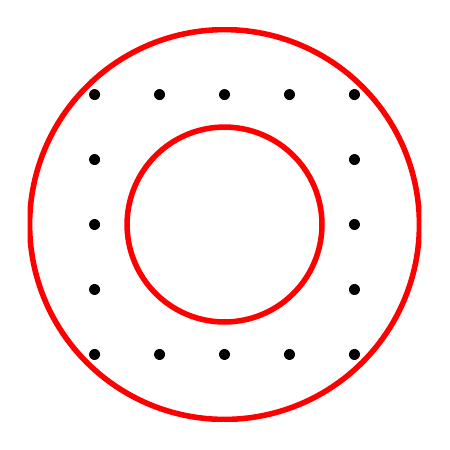
\begin{tikzpicture}

\begin{axis}[%
hide axis,
width=5cm,
height=5cm,
at={(0cm,0cm)},
scale only axis,
xmin=-10.1,
xmax=10.1,
ymin=-10.1,
ymax=10.1,
axis background/.style={fill=white},
]
\addplot [color=red, line width=2.0pt, forget plot]
  table[row sep=crcr]{%
10	0\\
9.99464587476366	-0.327190828217761\\
9.97858923238604	-0.654031292301431\\
9.95184726672197	-0.980171403295606\\
9.9144486137381	-1.30526192220052\\
9.86643332084879	-1.62895473394589\\
9.8078528040323	-1.95090322016128\\
9.73876979277334	-2.27076263034373\\
9.65925826289068	-2.58819045102521\\
9.56940335732209	-2.90284677254462\\
9.46930129495106	-3.21439465303162\\
9.35905926757326	-3.52250047921233\\
9.23879532511287	-3.8268343236509\\
9.10863824921176	-4.12707029804395\\
8.96872741532688	-4.42288690219001\\
8.81921264348355	-4.71396736825998\\
8.66025403784439	-5\\
8.49202181526579	-5.28067850650368\\
8.31469612302545	-5.55570233019602\\
8.12846684591615	-5.82477696867802\\
7.93353340291235	-6.08761429008721\\
7.73010453362737	-6.34393284163646\\
7.51839807478977	-6.59345815100069\\
7.29864072697836	-6.83592302022871\\
7.07106781186548	-7.07106781186547\\
6.83592302022871	-7.29864072697836\\
6.59345815100069	-7.51839807478977\\
6.34393284163646	-7.73010453362737\\
6.08761429008721	-7.93353340291235\\
5.82477696867802	-8.12846684591615\\
5.55570233019602	-8.31469612302545\\
5.28067850650368	-8.49202181526579\\
5	-8.66025403784439\\
4.71396736825998	-8.81921264348355\\
4.42288690219001	-8.96872741532688\\
4.12707029804395	-9.10863824921176\\
3.8268343236509	-9.23879532511287\\
3.52250047921234	-9.35905926757326\\
3.21439465303162	-9.46930129495106\\
2.90284677254462	-9.56940335732209\\
2.58819045102521	-9.65925826289068\\
2.27076263034373	-9.73876979277334\\
1.95090322016128	-9.8078528040323\\
1.62895473394589	-9.86643332084879\\
1.30526192220052	-9.9144486137381\\
0.980171403295605	-9.95184726672197\\
0.654031292301433	-9.97858923238604\\
0.327190828217762	-9.99464587476366\\
6.12323399573677e-16	-10\\
-0.32719082821776	-9.99464587476366\\
-0.654031292301431	-9.97858923238604\\
-0.980171403295604	-9.95184726672197\\
-1.30526192220052	-9.9144486137381\\
-1.62895473394589	-9.86643332084879\\
-1.95090322016128	-9.8078528040323\\
-2.27076263034373	-9.73876979277334\\
-2.58819045102521	-9.65925826289068\\
-2.90284677254462	-9.56940335732209\\
-3.21439465303162	-9.46930129495106\\
-3.52250047921233	-9.35905926757326\\
-3.8268343236509	-9.23879532511287\\
-4.12707029804395	-9.10863824921176\\
-4.42288690219001	-8.96872741532688\\
-4.71396736825998	-8.81921264348355\\
-5	-8.66025403784439\\
-5.28067850650368	-8.49202181526579\\
-5.55570233019602	-8.31469612302545\\
-5.82477696867802	-8.12846684591615\\
-6.08761429008721	-7.93353340291235\\
-6.34393284163645	-7.73010453362737\\
-6.59345815100069	-7.51839807478977\\
-6.83592302022871	-7.29864072697835\\
-7.07106781186547	-7.07106781186548\\
-7.29864072697835	-6.83592302022872\\
-7.51839807478977	-6.59345815100069\\
-7.73010453362737	-6.34393284163646\\
-7.93353340291235	-6.08761429008721\\
-8.12846684591615	-5.82477696867802\\
-8.31469612302545	-5.55570233019603\\
-8.49202181526579	-5.28067850650368\\
-8.66025403784439	-5\\
-8.81921264348355	-4.71396736825998\\
-8.96872741532688	-4.42288690219002\\
-9.10863824921176	-4.12707029804395\\
-9.23879532511287	-3.8268343236509\\
-9.35905926757326	-3.52250047921233\\
-9.46930129495106	-3.21439465303162\\
-9.56940335732209	-2.90284677254463\\
-9.65925826289068	-2.58819045102521\\
-9.73876979277334	-2.27076263034373\\
-9.8078528040323	-1.95090322016128\\
-9.86643332084879	-1.62895473394589\\
-9.9144486137381	-1.30526192220052\\
-9.95184726672197	-0.980171403295608\\
-9.97858923238604	-0.654031292301431\\
-9.99464587476366	-0.32719082821776\\
-10	-1.22464679914735e-15\\
-9.99464587476366	0.327190828217758\\
-9.97858923238604	0.654031292301429\\
-9.95184726672197	0.980171403295606\\
-9.9144486137381	1.30526192220052\\
-9.86643332084879	1.62895473394589\\
-9.80785280403231	1.95090322016128\\
-9.73876979277334	2.27076263034373\\
-9.65925826289068	2.58819045102521\\
-9.56940335732209	2.90284677254463\\
-9.46930129495106	3.21439465303162\\
-9.35905926757326	3.52250047921233\\
-9.23879532511287	3.8268343236509\\
-9.10863824921176	4.12707029804394\\
-8.96872741532688	4.42288690219001\\
-8.81921264348355	4.71396736825998\\
-8.66025403784439	5\\
-8.49202181526579	5.28067850650368\\
-8.31469612302545	5.55570233019602\\
-8.12846684591615	5.82477696867802\\
-7.93353340291235	6.08761429008721\\
-7.73010453362737	6.34393284163645\\
-7.51839807478977	6.59345815100069\\
-7.29864072697836	6.83592302022871\\
-7.07106781186548	7.07106781186547\\
-6.83592302022871	7.29864072697836\\
-6.59345815100069	7.51839807478977\\
-6.34393284163646	7.73010453362737\\
-6.08761429008721	7.93353340291235\\
-5.82477696867802	8.12846684591615\\
-5.55570233019602	8.31469612302545\\
-5.28067850650368	8.49202181526579\\
-5	8.66025403784439\\
-4.71396736825998	8.81921264348355\\
-4.42288690219001	8.96872741532688\\
-4.12707029804395	9.10863824921176\\
-3.8268343236509	9.23879532511287\\
-3.52250047921234	9.35905926757325\\
-3.21439465303162	9.46930129495106\\
-2.90284677254462	9.56940335732209\\
-2.58819045102521	9.65925826289068\\
-2.27076263034373	9.73876979277334\\
-1.95090322016129	9.8078528040323\\
-1.62895473394589	9.86643332084879\\
-1.30526192220052	9.9144486137381\\
-0.980171403295613	9.95184726672197\\
-0.654031292301427	9.97858923238604\\
-0.327190828217765	9.99464587476366\\
-1.83697019872103e-15	10\\
0.327190828217761	9.99464587476366\\
0.654031292301424	9.97858923238604\\
0.98017140329561	9.95184726672197\\
1.30526192220051	9.91444861373811\\
1.62895473394589	9.86643332084879\\
1.95090322016128	9.8078528040323\\
2.27076263034373	9.73876979277334\\
2.5881904510252	9.65925826289068\\
2.90284677254462	9.56940335732209\\
3.21439465303161	9.46930129495106\\
3.52250047921234	9.35905926757326\\
3.82683432365089	9.23879532511287\\
4.12707029804394	9.10863824921176\\
4.42288690219001	8.96872741532689\\
4.71396736825998	8.81921264348355\\
5	8.66025403784439\\
5.28067850650367	8.49202181526579\\
5.55570233019602	8.31469612302545\\
5.82477696867802	8.12846684591615\\
6.0876142900872	7.93353340291236\\
6.34393284163645	7.73010453362737\\
6.59345815100069	7.51839807478977\\
6.83592302022872	7.29864072697835\\
7.07106781186547	7.07106781186548\\
7.29864072697836	6.83592302022871\\
7.51839807478977	6.59345815100069\\
7.73010453362737	6.34393284163646\\
7.93353340291235	6.08761429008721\\
8.12846684591615	5.82477696867802\\
8.31469612302545	5.55570233019603\\
8.49202181526578	5.28067850650369\\
8.66025403784438	5\\
8.81921264348355	4.71396736825997\\
8.96872741532688	4.42288690219001\\
9.10863824921176	4.12707029804395\\
9.23879532511287	3.8268343236509\\
9.35905926757325	3.52250047921234\\
9.46930129495106	3.21439465303162\\
9.56940335732209	2.90284677254462\\
9.65925826289068	2.58819045102522\\
9.73876979277333	2.27076263034374\\
9.8078528040323	1.95090322016129\\
9.86643332084879	1.62895473394588\\
9.9144486137381	1.30526192220052\\
9.95184726672197	0.980171403295605\\
9.97858923238604	0.654031292301428\\
9.99464587476366	0.327190828217766\\
10	0\\
};
\addplot [color=red, line width=2.0pt, forget plot]
  table[row sep=crcr]{%
5	0\\
4.99732293738183	0.163595414108881\\
4.98929461619302	0.327015646150715\\
4.97592363336098	0.490085701647803\\
4.95722430686905	0.652630961100258\\
4.93321666042439	0.814477366972944\\
4.90392640201615	0.975451610080641\\
4.86938489638667	1.13538131517187\\
4.82962913144534	1.2940952255126\\
4.78470167866104	1.45142338627231\\
4.73465064747553	1.60719732651581\\
4.67952963378663	1.76125023960617\\
4.61939766255643	1.91341716182545\\
4.55431912460588	2.06353514902197\\
4.48436370766344	2.21144345109501\\
4.40960632174178	2.35698368412999\\
4.33012701892219	2.5\\
4.24601090763289	2.64033925325184\\
4.15734806151273	2.77785116509801\\
4.06423342295808	2.91238848433901\\
3.96676670145618	3.0438071450436\\
3.86505226681368	3.17196642081823\\
3.75919903739489	3.29672907550034\\
3.64932036348918	3.41796151011436\\
3.53553390593274	3.53553390593274\\
3.41796151011436	3.64932036348918\\
3.29672907550034	3.75919903739489\\
3.17196642081823	3.86505226681368\\
3.0438071450436	3.96676670145618\\
2.91238848433901	4.06423342295808\\
2.77785116509801	4.15734806151273\\
2.64033925325184	4.24601090763289\\
2.5	4.33012701892219\\
2.35698368412999	4.40960632174178\\
2.21144345109501	4.48436370766344\\
2.06353514902197	4.55431912460588\\
1.91341716182545	4.61939766255643\\
1.76125023960617	4.67952963378663\\
1.60719732651581	4.73465064747553\\
1.45142338627231	4.78470167866104\\
1.2940952255126	4.82962913144534\\
1.13538131517187	4.86938489638667\\
0.975451610080642	4.90392640201615\\
0.814477366972944	4.93321666042439\\
0.652630961100259	4.95722430686905\\
0.490085701647803	4.97592363336098\\
0.327015646150716	4.98929461619302\\
0.163595414108881	4.99732293738183\\
3.06161699786838e-16	5\\
-0.16359541410888	4.99732293738183\\
-0.327015646150716	4.98929461619302\\
-0.490085701647802	4.97592363336098\\
-0.652630961100258	4.95722430686905\\
-0.814477366972943	4.93321666042439\\
-0.975451610080641	4.90392640201615\\
-1.13538131517187	4.86938489638667\\
-1.2940952255126	4.82962913144534\\
-1.45142338627231	4.78470167866104\\
-1.60719732651581	4.73465064747553\\
-1.76125023960617	4.67952963378663\\
-1.91341716182545	4.61939766255643\\
-2.06353514902197	4.55431912460588\\
-2.21144345109501	4.48436370766344\\
-2.35698368412999	4.40960632174178\\
-2.5	4.33012701892219\\
-2.64033925325184	4.24601090763289\\
-2.77785116509801	4.15734806151273\\
-2.91238848433901	4.06423342295808\\
-3.0438071450436	3.96676670145618\\
-3.17196642081823	3.86505226681369\\
-3.29672907550034	3.75919903739489\\
-3.41796151011436	3.64932036348918\\
-3.53553390593274	3.53553390593274\\
-3.64932036348918	3.41796151011436\\
-3.75919903739489	3.29672907550034\\
-3.86505226681368	3.17196642081823\\
-3.96676670145618	3.0438071450436\\
-4.06423342295808	2.91238848433901\\
-4.15734806151273	2.77785116509801\\
-4.24601090763289	2.64033925325184\\
-4.33012701892219	2.5\\
-4.40960632174177	2.35698368412999\\
-4.48436370766344	2.21144345109501\\
-4.55431912460588	2.06353514902197\\
-4.61939766255643	1.91341716182545\\
-4.67952963378663	1.76125023960617\\
-4.73465064747553	1.60719732651581\\
-4.78470167866104	1.45142338627231\\
-4.82962913144534	1.29409522551261\\
-4.86938489638667	1.13538131517187\\
-4.90392640201615	0.975451610080641\\
-4.93321666042439	0.814477366972944\\
-4.95722430686905	0.65263096110026\\
-4.97592363336098	0.490085701647804\\
-4.98929461619302	0.327015646150716\\
-4.99732293738183	0.16359541410888\\
-5	6.12323399573677e-16\\
-4.99732293738183	-0.163595414108879\\
-4.98929461619302	-0.327015646150714\\
-4.97592363336098	-0.490085701647803\\
-4.95722430686905	-0.652630961100259\\
-4.93321666042439	-0.814477366972943\\
-4.90392640201615	-0.97545161008064\\
-4.86938489638667	-1.13538131517187\\
-4.82962913144534	-1.2940952255126\\
-4.78470167866104	-1.45142338627231\\
-4.73465064747553	-1.60719732651581\\
-4.67952963378663	-1.76125023960617\\
-4.61939766255643	-1.91341716182545\\
-4.55431912460588	-2.06353514902197\\
-4.48436370766344	-2.21144345109501\\
-4.40960632174178	-2.35698368412999\\
-4.33012701892219	-2.5\\
-4.2460109076329	-2.64033925325184\\
-4.15734806151273	-2.77785116509801\\
-4.06423342295808	-2.91238848433901\\
-3.96676670145618	-3.0438071450436\\
-3.86505226681369	-3.17196642081823\\
-3.75919903739489	-3.29672907550034\\
-3.64932036348918	-3.41796151011436\\
-3.53553390593274	-3.53553390593274\\
-3.41796151011436	-3.64932036348918\\
-3.29672907550035	-3.75919903739489\\
-3.17196642081823	-3.86505226681368\\
-3.0438071450436	-3.96676670145617\\
-2.91238848433901	-4.06423342295808\\
-2.77785116509801	-4.15734806151273\\
-2.64033925325184	-4.2460109076329\\
-2.5	-4.33012701892219\\
-2.35698368412999	-4.40960632174177\\
-2.21144345109501	-4.48436370766344\\
-2.06353514902197	-4.55431912460588\\
-1.91341716182545	-4.61939766255643\\
-1.76125023960617	-4.67952963378663\\
-1.60719732651581	-4.73465064747553\\
-1.45142338627231	-4.78470167866104\\
-1.2940952255126	-4.82962913144534\\
-1.13538131517186	-4.86938489638667\\
-0.975451610080643	-4.90392640201615\\
-0.814477366972945	-4.93321666042439\\
-0.652630961100258	-4.95722430686905\\
-0.490085701647807	-4.97592363336098\\
-0.327015646150714	-4.98929461619302\\
-0.163595414108883	-4.99732293738183\\
-9.18485099360515e-16	-5\\
0.163595414108881	-4.99732293738183\\
0.327015646150712	-4.98929461619302\\
0.490085701647805	-4.97592363336098\\
0.652630961100256	-4.95722430686905\\
0.814477366972943	-4.93321666042439\\
0.975451610080642	-4.90392640201615\\
1.13538131517186	-4.86938489638667\\
1.2940952255126	-4.82962913144534\\
1.45142338627231	-4.78470167866104\\
1.60719732651581	-4.73465064747553\\
1.76125023960617	-4.67952963378663\\
1.91341716182545	-4.61939766255643\\
2.06353514902197	-4.55431912460588\\
2.211443451095	-4.48436370766344\\
2.35698368412999	-4.40960632174178\\
2.5	-4.33012701892219\\
2.64033925325184	-4.2460109076329\\
2.77785116509801	-4.15734806151273\\
2.91238848433901	-4.06423342295808\\
3.0438071450436	-3.96676670145618\\
3.17196642081822	-3.86505226681369\\
3.29672907550035	-3.75919903739489\\
3.41796151011436	-3.64932036348918\\
3.53553390593274	-3.53553390593274\\
3.64932036348918	-3.41796151011436\\
3.75919903739489	-3.29672907550034\\
3.86505226681368	-3.17196642081823\\
3.96676670145617	-3.0438071450436\\
4.06423342295808	-2.91238848433901\\
4.15734806151272	-2.77785116509801\\
4.24601090763289	-2.64033925325184\\
4.33012701892219	-2.5\\
4.40960632174178	-2.35698368412999\\
4.48436370766344	-2.21144345109501\\
4.55431912460588	-2.06353514902197\\
4.61939766255643	-1.91341716182545\\
4.67952963378663	-1.76125023960617\\
4.73465064747553	-1.60719732651581\\
4.78470167866104	-1.45142338627231\\
4.82962913144534	-1.29409522551261\\
4.86938489638667	-1.13538131517187\\
4.90392640201615	-0.975451610080644\\
4.9332166604244	-0.814477366972941\\
4.95722430686905	-0.652630961100258\\
4.97592363336098	-0.490085701647803\\
4.98929461619302	-0.327015646150714\\
4.99732293738183	-0.163595414108883\\
5	0\\
};

\addplot[area legend, draw=black, fill=black, forget plot]
table[row sep=crcr] {%
x	y\\
-6.41666666666667	-6.66666666666667\\
-6.42147034656586	-6.61789408616263\\
-6.43569678353884	-6.57099580857539\\
-6.45879926359103	-6.52777410841177\\
-6.48988997137003	-6.48988997137003\\
-6.52777410841177	-6.45879926359103\\
-6.57099580857539	-6.43569678353884\\
-6.61789408616263	-6.42147034656586\\
-6.66666666666667	-6.41666666666667\\
-6.7154392471707	-6.42147034656586\\
-6.76233752475794	-6.43569678353884\\
-6.80555922492157	-6.45879926359103\\
-6.8434433619633	-6.48988997137003\\
-6.8745340697423	-6.52777410841177\\
-6.89763654979449	-6.57099580857539\\
-6.91186298676747	-6.61789408616263\\
-6.91666666666667	-6.66666666666667\\
-6.91186298676747	-6.7154392471707\\
-6.89763654979449	-6.76233752475794\\
-6.8745340697423	-6.80555922492157\\
-6.8434433619633	-6.8434433619633\\
-6.80555922492157	-6.8745340697423\\
-6.76233752475794	-6.89763654979449\\
-6.7154392471707	-6.91186298676747\\
-6.66666666666667	-6.91666666666667\\
-6.61789408616263	-6.91186298676747\\
-6.57099580857539	-6.89763654979449\\
-6.52777410841177	-6.8745340697423\\
-6.48988997137003	-6.8434433619633\\
-6.45879926359103	-6.80555922492157\\
-6.43569678353884	-6.76233752475794\\
-6.42147034656586	-6.7154392471707\\
-6.41666666666667	-6.66666666666667\\
}--cycle;

\addplot[area legend, draw=black, fill=black, forget plot]
table[row sep=crcr] {%
x	y\\
-3.08333333333333	-6.66666666666667\\
-3.08813701323253	-6.61789408616263\\
-3.10236345020551	-6.57099580857539\\
-3.1254659302577	-6.52777410841177\\
-3.1565566380367	-6.48988997137003\\
-3.19444077507843	-6.45879926359103\\
-3.23766247524206	-6.43569678353884\\
-3.2845607528293	-6.42147034656586\\
-3.33333333333333	-6.41666666666667\\
-3.38210591383737	-6.42147034656586\\
-3.42900419142461	-6.43569678353884\\
-3.47222589158823	-6.45879926359103\\
-3.51011002862997	-6.48988997137003\\
-3.54120073640897	-6.52777410841177\\
-3.56430321646115	-6.57099580857539\\
-3.57852965343414	-6.61789408616263\\
-3.58333333333333	-6.66666666666667\\
-3.57852965343414	-6.7154392471707\\
-3.56430321646115	-6.76233752475794\\
-3.54120073640897	-6.80555922492157\\
-3.51011002862997	-6.8434433619633\\
-3.47222589158823	-6.8745340697423\\
-3.42900419142461	-6.89763654979449\\
-3.38210591383737	-6.91186298676747\\
-3.33333333333333	-6.91666666666667\\
-3.2845607528293	-6.91186298676747\\
-3.23766247524206	-6.89763654979449\\
-3.19444077507843	-6.8745340697423\\
-3.1565566380367	-6.8434433619633\\
-3.1254659302577	-6.80555922492157\\
-3.10236345020551	-6.76233752475794\\
-3.08813701323253	-6.7154392471707\\
-3.08333333333333	-6.66666666666667\\
}--cycle;

\addplot[area legend, draw=black, fill=black, forget plot]
table[row sep=crcr] {%
x	y\\
0.25	-6.66666666666667\\
0.245196320100808	-6.61789408616263\\
0.230969883127822	-6.57099580857539\\
0.207867403075636	-6.52777410841177\\
0.176776695296637	-6.48988997137003\\
0.138892558254901	-6.45879926359103\\
0.0956708580912725	-6.43569678353884\\
0.0487725805040321	-6.42147034656586\\
1.53080849893419e-17	-6.41666666666667\\
-0.048772580504032	-6.42147034656586\\
-0.0956708580912724	-6.43569678353884\\
-0.138892558254901	-6.45879926359103\\
-0.176776695296637	-6.48988997137003\\
-0.207867403075636	-6.52777410841177\\
-0.230969883127822	-6.57099580857539\\
-0.245196320100808	-6.61789408616263\\
-0.25	-6.66666666666667\\
-0.245196320100808	-6.7154392471707\\
-0.230969883127822	-6.76233752475794\\
-0.207867403075636	-6.80555922492157\\
-0.176776695296637	-6.8434433619633\\
-0.138892558254901	-6.8745340697423\\
-0.0956708580912726	-6.89763654979449\\
-0.0487725805040322	-6.91186298676747\\
-4.59242549680257e-17	-6.91666666666667\\
0.0487725805040321	-6.91186298676747\\
0.0956708580912725	-6.89763654979449\\
0.1388925582549	-6.8745340697423\\
0.176776695296637	-6.8434433619633\\
0.207867403075636	-6.80555922492157\\
0.230969883127822	-6.76233752475794\\
0.245196320100808	-6.7154392471707\\
0.25	-6.66666666666667\\
}--cycle;

\addplot[area legend, draw=black, fill=black, forget plot]
table[row sep=crcr] {%
x	y\\
3.58333333333333	-6.66666666666667\\
3.57852965343414	-6.61789408616263\\
3.56430321646116	-6.57099580857539\\
3.54120073640897	-6.52777410841177\\
3.51011002862997	-6.48988997137003\\
3.47222589158823	-6.45879926359103\\
3.42900419142461	-6.43569678353884\\
3.38210591383737	-6.42147034656586\\
3.33333333333333	-6.41666666666667\\
3.2845607528293	-6.42147034656586\\
3.23766247524206	-6.43569678353884\\
3.19444077507843	-6.45879926359103\\
3.1565566380367	-6.48988997137003\\
3.1254659302577	-6.52777410841177\\
3.10236345020551	-6.57099580857539\\
3.08813701323253	-6.61789408616263\\
3.08333333333333	-6.66666666666667\\
3.08813701323253	-6.7154392471707\\
3.10236345020551	-6.76233752475794\\
3.1254659302577	-6.80555922492157\\
3.1565566380367	-6.8434433619633\\
3.19444077507843	-6.8745340697423\\
3.23766247524206	-6.89763654979449\\
3.2845607528293	-6.91186298676747\\
3.33333333333333	-6.91666666666667\\
3.38210591383737	-6.91186298676747\\
3.42900419142461	-6.89763654979449\\
3.47222589158823	-6.8745340697423\\
3.51011002862997	-6.8434433619633\\
3.54120073640897	-6.80555922492157\\
3.56430321646116	-6.76233752475794\\
3.57852965343414	-6.7154392471707\\
3.58333333333333	-6.66666666666667\\
}--cycle;

\addplot[area legend, draw=black, fill=black, forget plot]
table[row sep=crcr] {%
x	y\\
6.91666666666667	-6.66666666666667\\
6.91186298676748	-6.61789408616263\\
6.89763654979449	-6.57099580857539\\
6.8745340697423	-6.52777410841177\\
6.8434433619633	-6.48988997137003\\
6.80555922492157	-6.45879926359103\\
6.76233752475794	-6.43569678353884\\
6.7154392471707	-6.42147034656586\\
6.66666666666667	-6.41666666666667\\
6.61789408616264	-6.42147034656586\\
6.5709958085754	-6.43569678353884\\
6.52777410841177	-6.45879926359103\\
6.48988997137003	-6.48988997137003\\
6.45879926359103	-6.52777410841177\\
6.43569678353885	-6.57099580857539\\
6.42147034656586	-6.61789408616263\\
6.41666666666667	-6.66666666666667\\
6.42147034656586	-6.7154392471707\\
6.43569678353885	-6.76233752475794\\
6.45879926359103	-6.80555922492157\\
6.48988997137003	-6.8434433619633\\
6.52777410841177	-6.8745340697423\\
6.5709958085754	-6.89763654979449\\
6.61789408616264	-6.91186298676747\\
6.66666666666667	-6.91666666666667\\
6.7154392471707	-6.91186298676747\\
6.76233752475794	-6.89763654979449\\
6.80555922492157	-6.8745340697423\\
6.8434433619633	-6.8434433619633\\
6.8745340697423	-6.80555922492157\\
6.89763654979449	-6.76233752475794\\
6.91186298676748	-6.7154392471707\\
6.91666666666667	-6.66666666666667\\
}--cycle;

\addplot[area legend, draw=black, fill=black, forget plot]
table[row sep=crcr] {%
x	y\\
-6.41666666666667	-3.33333333333333\\
-6.42147034656586	-3.2845607528293\\
-6.43569678353884	-3.23766247524206\\
-6.45879926359103	-3.19444077507843\\
-6.48988997137003	-3.1565566380367\\
-6.52777410841177	-3.1254659302577\\
-6.57099580857539	-3.10236345020551\\
-6.61789408616263	-3.08813701323253\\
-6.66666666666667	-3.08333333333333\\
-6.7154392471707	-3.08813701323253\\
-6.76233752475794	-3.10236345020551\\
-6.80555922492157	-3.1254659302577\\
-6.8434433619633	-3.1565566380367\\
-6.8745340697423	-3.19444077507843\\
-6.89763654979449	-3.23766247524206\\
-6.91186298676747	-3.2845607528293\\
-6.91666666666667	-3.33333333333333\\
-6.91186298676747	-3.38210591383737\\
-6.89763654979449	-3.42900419142461\\
-6.8745340697423	-3.47222589158823\\
-6.8434433619633	-3.51011002862997\\
-6.80555922492157	-3.54120073640897\\
-6.76233752475794	-3.56430321646115\\
-6.7154392471707	-3.57852965343414\\
-6.66666666666667	-3.58333333333333\\
-6.61789408616263	-3.57852965343414\\
-6.57099580857539	-3.56430321646115\\
-6.52777410841177	-3.54120073640897\\
-6.48988997137003	-3.51011002862997\\
-6.45879926359103	-3.47222589158823\\
-6.43569678353884	-3.42900419142461\\
-6.42147034656586	-3.38210591383737\\
-6.41666666666667	-3.33333333333333\\
}--cycle;

\addplot[area legend, draw=black, fill=black, forget plot]
table[row sep=crcr] {%
x	y\\
6.91666666666667	-3.33333333333333\\
6.91186298676748	-3.2845607528293\\
6.89763654979449	-3.23766247524206\\
6.8745340697423	-3.19444077507843\\
6.8434433619633	-3.1565566380367\\
6.80555922492157	-3.1254659302577\\
6.76233752475794	-3.10236345020551\\
6.7154392471707	-3.08813701323253\\
6.66666666666667	-3.08333333333333\\
6.61789408616264	-3.08813701323253\\
6.5709958085754	-3.10236345020551\\
6.52777410841177	-3.1254659302577\\
6.48988997137003	-3.1565566380367\\
6.45879926359103	-3.19444077507843\\
6.43569678353885	-3.23766247524206\\
6.42147034656586	-3.2845607528293\\
6.41666666666667	-3.33333333333333\\
6.42147034656586	-3.38210591383737\\
6.43569678353885	-3.42900419142461\\
6.45879926359103	-3.47222589158823\\
6.48988997137003	-3.51011002862997\\
6.52777410841177	-3.54120073640897\\
6.5709958085754	-3.56430321646115\\
6.61789408616264	-3.57852965343414\\
6.66666666666667	-3.58333333333333\\
6.7154392471707	-3.57852965343414\\
6.76233752475794	-3.56430321646115\\
6.80555922492157	-3.54120073640897\\
6.8434433619633	-3.51011002862997\\
6.8745340697423	-3.47222589158823\\
6.89763654979449	-3.42900419142461\\
6.91186298676748	-3.38210591383737\\
6.91666666666667	-3.33333333333333\\
}--cycle;

\addplot[area legend, draw=black, fill=black, forget plot]
table[row sep=crcr] {%
x	y\\
-6.41666666666667	0\\
-6.42147034656586	0.0487725805040321\\
-6.43569678353884	0.0956708580912724\\
-6.45879926359103	0.138892558254901\\
-6.48988997137003	0.176776695296637\\
-6.52777410841177	0.207867403075636\\
-6.57099580857539	0.230969883127822\\
-6.61789408616263	0.245196320100808\\
-6.66666666666667	0.25\\
-6.7154392471707	0.245196320100808\\
-6.76233752475794	0.230969883127822\\
-6.80555922492157	0.207867403075636\\
-6.8434433619633	0.176776695296637\\
-6.8745340697423	0.138892558254901\\
-6.89763654979449	0.0956708580912725\\
-6.91186298676747	0.0487725805040321\\
-6.91666666666667	3.06161699786838e-17\\
-6.91186298676747	-0.0487725805040321\\
-6.89763654979449	-0.0956708580912724\\
-6.8745340697423	-0.1388925582549\\
-6.8434433619633	-0.176776695296637\\
-6.80555922492157	-0.207867403075636\\
-6.76233752475794	-0.230969883127822\\
-6.7154392471707	-0.245196320100808\\
-6.66666666666667	-0.25\\
-6.61789408616263	-0.245196320100808\\
-6.57099580857539	-0.230969883127822\\
-6.52777410841177	-0.207867403075636\\
-6.48988997137003	-0.176776695296637\\
-6.45879926359103	-0.138892558254901\\
-6.43569678353884	-0.0956708580912726\\
-6.42147034656586	-0.0487725805040322\\
-6.41666666666667	0\\
}--cycle;

\addplot[area legend, draw=black, fill=black, forget plot]
table[row sep=crcr] {%
x	y\\
6.91666666666667	0\\
6.91186298676748	0.0487725805040321\\
6.89763654979449	0.0956708580912724\\
6.8745340697423	0.138892558254901\\
6.8434433619633	0.176776695296637\\
6.80555922492157	0.207867403075636\\
6.76233752475794	0.230969883127822\\
6.7154392471707	0.245196320100808\\
6.66666666666667	0.25\\
6.61789408616264	0.245196320100808\\
6.5709958085754	0.230969883127822\\
6.52777410841177	0.207867403075636\\
6.48988997137003	0.176776695296637\\
6.45879926359103	0.138892558254901\\
6.43569678353885	0.0956708580912725\\
6.42147034656586	0.0487725805040321\\
6.41666666666667	3.06161699786838e-17\\
6.42147034656586	-0.0487725805040321\\
6.43569678353885	-0.0956708580912724\\
6.45879926359103	-0.1388925582549\\
6.48988997137003	-0.176776695296637\\
6.52777410841177	-0.207867403075636\\
6.5709958085754	-0.230969883127822\\
6.61789408616264	-0.245196320100808\\
6.66666666666667	-0.25\\
6.7154392471707	-0.245196320100808\\
6.76233752475794	-0.230969883127822\\
6.80555922492157	-0.207867403075636\\
6.8434433619633	-0.176776695296637\\
6.8745340697423	-0.138892558254901\\
6.89763654979449	-0.0956708580912726\\
6.91186298676748	-0.0487725805040322\\
6.91666666666667	0\\
}--cycle;

\addplot[area legend, draw=black, fill=black, forget plot]
table[row sep=crcr] {%
x	y\\
-6.41666666666667	3.33333333333333\\
-6.42147034656586	3.38210591383737\\
-6.43569678353884	3.42900419142461\\
-6.45879926359103	3.47222589158823\\
-6.48988997137003	3.51011002862997\\
-6.52777410841177	3.54120073640897\\
-6.57099580857539	3.56430321646116\\
-6.61789408616263	3.57852965343414\\
-6.66666666666667	3.58333333333333\\
-6.7154392471707	3.57852965343414\\
-6.76233752475794	3.56430321646116\\
-6.80555922492157	3.54120073640897\\
-6.8434433619633	3.51011002862997\\
-6.8745340697423	3.47222589158823\\
-6.89763654979449	3.42900419142461\\
-6.91186298676747	3.38210591383737\\
-6.91666666666667	3.33333333333333\\
-6.91186298676747	3.2845607528293\\
-6.89763654979449	3.23766247524206\\
-6.8745340697423	3.19444077507843\\
-6.8434433619633	3.1565566380367\\
-6.80555922492157	3.1254659302577\\
-6.76233752475794	3.10236345020551\\
-6.7154392471707	3.08813701323253\\
-6.66666666666667	3.08333333333333\\
-6.61789408616263	3.08813701323253\\
-6.57099580857539	3.10236345020551\\
-6.52777410841177	3.1254659302577\\
-6.48988997137003	3.1565566380367\\
-6.45879926359103	3.19444077507843\\
-6.43569678353884	3.23766247524206\\
-6.42147034656586	3.2845607528293\\
-6.41666666666667	3.33333333333333\\
}--cycle;

\addplot[area legend, draw=black, fill=black, forget plot]
table[row sep=crcr] {%
x	y\\
6.91666666666667	3.33333333333333\\
6.91186298676748	3.38210591383737\\
6.89763654979449	3.42900419142461\\
6.8745340697423	3.47222589158823\\
6.8434433619633	3.51011002862997\\
6.80555922492157	3.54120073640897\\
6.76233752475794	3.56430321646116\\
6.7154392471707	3.57852965343414\\
6.66666666666667	3.58333333333333\\
6.61789408616264	3.57852965343414\\
6.5709958085754	3.56430321646116\\
6.52777410841177	3.54120073640897\\
6.48988997137003	3.51011002862997\\
6.45879926359103	3.47222589158823\\
6.43569678353885	3.42900419142461\\
6.42147034656586	3.38210591383737\\
6.41666666666667	3.33333333333333\\
6.42147034656586	3.2845607528293\\
6.43569678353885	3.23766247524206\\
6.45879926359103	3.19444077507843\\
6.48988997137003	3.1565566380367\\
6.52777410841177	3.1254659302577\\
6.5709958085754	3.10236345020551\\
6.61789408616264	3.08813701323253\\
6.66666666666667	3.08333333333333\\
6.7154392471707	3.08813701323253\\
6.76233752475794	3.10236345020551\\
6.80555922492157	3.1254659302577\\
6.8434433619633	3.1565566380367\\
6.8745340697423	3.19444077507843\\
6.89763654979449	3.23766247524206\\
6.91186298676748	3.2845607528293\\
6.91666666666667	3.33333333333333\\
}--cycle;

\addplot[area legend, draw=black, fill=black, forget plot]
table[row sep=crcr] {%
x	y\\
-6.41666666666667	6.66666666666667\\
-6.42147034656586	6.7154392471707\\
-6.43569678353884	6.76233752475794\\
-6.45879926359103	6.80555922492157\\
-6.48988997137003	6.8434433619633\\
-6.52777410841177	6.8745340697423\\
-6.57099580857539	6.89763654979449\\
-6.61789408616263	6.91186298676748\\
-6.66666666666667	6.91666666666667\\
-6.7154392471707	6.91186298676748\\
-6.76233752475794	6.89763654979449\\
-6.80555922492157	6.8745340697423\\
-6.8434433619633	6.8434433619633\\
-6.8745340697423	6.80555922492157\\
-6.89763654979449	6.76233752475794\\
-6.91186298676747	6.7154392471707\\
-6.91666666666667	6.66666666666667\\
-6.91186298676747	6.61789408616264\\
-6.89763654979449	6.5709958085754\\
-6.8745340697423	6.52777410841177\\
-6.8434433619633	6.48988997137003\\
-6.80555922492157	6.45879926359103\\
-6.76233752475794	6.43569678353885\\
-6.7154392471707	6.42147034656586\\
-6.66666666666667	6.41666666666667\\
-6.61789408616263	6.42147034656586\\
-6.57099580857539	6.43569678353885\\
-6.52777410841177	6.45879926359103\\
-6.48988997137003	6.48988997137003\\
-6.45879926359103	6.52777410841177\\
-6.43569678353884	6.5709958085754\\
-6.42147034656586	6.61789408616264\\
-6.41666666666667	6.66666666666667\\
}--cycle;

\addplot[area legend, draw=black, fill=black, forget plot]
table[row sep=crcr] {%
x	y\\
-3.08333333333333	6.66666666666667\\
-3.08813701323253	6.7154392471707\\
-3.10236345020551	6.76233752475794\\
-3.1254659302577	6.80555922492157\\
-3.1565566380367	6.8434433619633\\
-3.19444077507843	6.8745340697423\\
-3.23766247524206	6.89763654979449\\
-3.2845607528293	6.91186298676748\\
-3.33333333333333	6.91666666666667\\
-3.38210591383737	6.91186298676748\\
-3.42900419142461	6.89763654979449\\
-3.47222589158823	6.8745340697423\\
-3.51011002862997	6.8434433619633\\
-3.54120073640897	6.80555922492157\\
-3.56430321646115	6.76233752475794\\
-3.57852965343414	6.7154392471707\\
-3.58333333333333	6.66666666666667\\
-3.57852965343414	6.61789408616264\\
-3.56430321646115	6.5709958085754\\
-3.54120073640897	6.52777410841177\\
-3.51011002862997	6.48988997137003\\
-3.47222589158823	6.45879926359103\\
-3.42900419142461	6.43569678353885\\
-3.38210591383737	6.42147034656586\\
-3.33333333333333	6.41666666666667\\
-3.2845607528293	6.42147034656586\\
-3.23766247524206	6.43569678353885\\
-3.19444077507843	6.45879926359103\\
-3.1565566380367	6.48988997137003\\
-3.1254659302577	6.52777410841177\\
-3.10236345020551	6.5709958085754\\
-3.08813701323253	6.61789408616264\\
-3.08333333333333	6.66666666666667\\
}--cycle;

\addplot[area legend, draw=black, fill=black, forget plot]
table[row sep=crcr] {%
x	y\\
0.25	6.66666666666667\\
0.245196320100808	6.7154392471707\\
0.230969883127822	6.76233752475794\\
0.207867403075636	6.80555922492157\\
0.176776695296637	6.8434433619633\\
0.138892558254901	6.8745340697423\\
0.0956708580912725	6.89763654979449\\
0.0487725805040321	6.91186298676748\\
1.53080849893419e-17	6.91666666666667\\
-0.048772580504032	6.91186298676748\\
-0.0956708580912724	6.89763654979449\\
-0.138892558254901	6.8745340697423\\
-0.176776695296637	6.8434433619633\\
-0.207867403075636	6.80555922492157\\
-0.230969883127822	6.76233752475794\\
-0.245196320100808	6.7154392471707\\
-0.25	6.66666666666667\\
-0.245196320100808	6.61789408616264\\
-0.230969883127822	6.5709958085754\\
-0.207867403075636	6.52777410841177\\
-0.176776695296637	6.48988997137003\\
-0.138892558254901	6.45879926359103\\
-0.0956708580912726	6.43569678353885\\
-0.0487725805040322	6.42147034656586\\
-4.59242549680257e-17	6.41666666666667\\
0.0487725805040321	6.42147034656586\\
0.0956708580912725	6.43569678353885\\
0.1388925582549	6.45879926359103\\
0.176776695296637	6.48988997137003\\
0.207867403075636	6.52777410841177\\
0.230969883127822	6.5709958085754\\
0.245196320100808	6.61789408616264\\
0.25	6.66666666666667\\
}--cycle;

\addplot[area legend, draw=black, fill=black, forget plot]
table[row sep=crcr] {%
x	y\\
3.58333333333333	6.66666666666667\\
3.57852965343414	6.7154392471707\\
3.56430321646116	6.76233752475794\\
3.54120073640897	6.80555922492157\\
3.51011002862997	6.8434433619633\\
3.47222589158823	6.8745340697423\\
3.42900419142461	6.89763654979449\\
3.38210591383737	6.91186298676748\\
3.33333333333333	6.91666666666667\\
3.2845607528293	6.91186298676748\\
3.23766247524206	6.89763654979449\\
3.19444077507843	6.8745340697423\\
3.1565566380367	6.8434433619633\\
3.1254659302577	6.80555922492157\\
3.10236345020551	6.76233752475794\\
3.08813701323253	6.7154392471707\\
3.08333333333333	6.66666666666667\\
3.08813701323253	6.61789408616264\\
3.10236345020551	6.5709958085754\\
3.1254659302577	6.52777410841177\\
3.1565566380367	6.48988997137003\\
3.19444077507843	6.45879926359103\\
3.23766247524206	6.43569678353885\\
3.2845607528293	6.42147034656586\\
3.33333333333333	6.41666666666667\\
3.38210591383737	6.42147034656586\\
3.42900419142461	6.43569678353885\\
3.47222589158823	6.45879926359103\\
3.51011002862997	6.48988997137003\\
3.54120073640897	6.52777410841177\\
3.56430321646116	6.5709958085754\\
3.57852965343414	6.61789408616264\\
3.58333333333333	6.66666666666667\\
}--cycle;

\addplot[area legend, draw=black, fill=black, forget plot]
table[row sep=crcr] {%
x	y\\
6.91666666666667	6.66666666666667\\
6.91186298676748	6.7154392471707\\
6.89763654979449	6.76233752475794\\
6.8745340697423	6.80555922492157\\
6.8434433619633	6.8434433619633\\
6.80555922492157	6.8745340697423\\
6.76233752475794	6.89763654979449\\
6.7154392471707	6.91186298676748\\
6.66666666666667	6.91666666666667\\
6.61789408616264	6.91186298676748\\
6.5709958085754	6.89763654979449\\
6.52777410841177	6.8745340697423\\
6.48988997137003	6.8434433619633\\
6.45879926359103	6.80555922492157\\
6.43569678353885	6.76233752475794\\
6.42147034656586	6.7154392471707\\
6.41666666666667	6.66666666666667\\
6.42147034656586	6.61789408616264\\
6.43569678353885	6.5709958085754\\
6.45879926359103	6.52777410841177\\
6.48988997137003	6.48988997137003\\
6.52777410841177	6.45879926359103\\
6.5709958085754	6.43569678353885\\
6.61789408616264	6.42147034656586\\
6.66666666666667	6.41666666666667\\
6.7154392471707	6.42147034656586\\
6.76233752475794	6.43569678353885\\
6.80555922492157	6.45879926359103\\
6.8434433619633	6.48988997137003\\
6.8745340697423	6.52777410841177\\
6.89763654979449	6.5709958085754\\
6.91186298676748	6.61789408616264\\
6.91666666666667	6.66666666666667\\
}--cycle;
\end{axis}
\end{tikzpicture}% & % This file was created by matlab2tikz.
%
%The latest updates can be retrieved from
%  http://www.mathworks.com/matlabcentral/fileexchange/22022-matlab2tikz-matlab2tikz
%where you can also make suggestions and rate matlab2tikz.
%
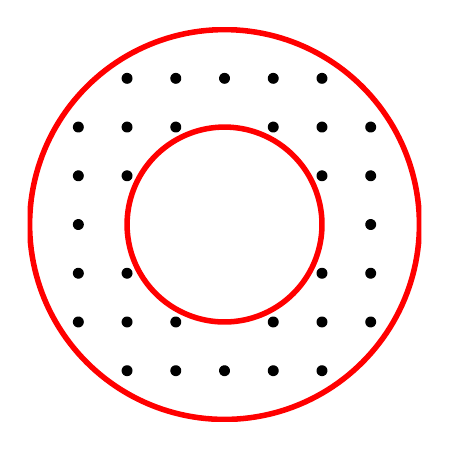
\begin{tikzpicture}

\begin{axis}[%
hide axis,
width=5cm,
height=5cm,
at={(0cm,0cm)},
scale only axis,
xmin=-10.1,
xmax=10.1,
ymin=-10.1,
ymax=10.1,
axis background/.style={fill=white},
]
\addplot [color=red, line width=2.0pt, forget plot]
  table[row sep=crcr]{%
10	0\\
9.99464587476366	-0.327190828217761\\
9.97858923238604	-0.654031292301431\\
9.95184726672197	-0.980171403295606\\
9.9144486137381	-1.30526192220052\\
9.86643332084879	-1.62895473394589\\
9.8078528040323	-1.95090322016128\\
9.73876979277334	-2.27076263034373\\
9.65925826289068	-2.58819045102521\\
9.56940335732209	-2.90284677254462\\
9.46930129495106	-3.21439465303162\\
9.35905926757326	-3.52250047921233\\
9.23879532511287	-3.8268343236509\\
9.10863824921176	-4.12707029804395\\
8.96872741532688	-4.42288690219001\\
8.81921264348355	-4.71396736825998\\
8.66025403784439	-5\\
8.49202181526579	-5.28067850650368\\
8.31469612302545	-5.55570233019602\\
8.12846684591615	-5.82477696867802\\
7.93353340291235	-6.08761429008721\\
7.73010453362737	-6.34393284163646\\
7.51839807478977	-6.59345815100069\\
7.29864072697836	-6.83592302022871\\
7.07106781186548	-7.07106781186547\\
6.83592302022871	-7.29864072697836\\
6.59345815100069	-7.51839807478977\\
6.34393284163646	-7.73010453362737\\
6.08761429008721	-7.93353340291235\\
5.82477696867802	-8.12846684591615\\
5.55570233019602	-8.31469612302545\\
5.28067850650368	-8.49202181526579\\
5	-8.66025403784439\\
4.71396736825998	-8.81921264348355\\
4.42288690219001	-8.96872741532688\\
4.12707029804395	-9.10863824921176\\
3.8268343236509	-9.23879532511287\\
3.52250047921234	-9.35905926757326\\
3.21439465303162	-9.46930129495106\\
2.90284677254462	-9.56940335732209\\
2.58819045102521	-9.65925826289068\\
2.27076263034373	-9.73876979277334\\
1.95090322016128	-9.8078528040323\\
1.62895473394589	-9.86643332084879\\
1.30526192220052	-9.9144486137381\\
0.980171403295605	-9.95184726672197\\
0.654031292301433	-9.97858923238604\\
0.327190828217762	-9.99464587476366\\
6.12323399573677e-16	-10\\
-0.32719082821776	-9.99464587476366\\
-0.654031292301431	-9.97858923238604\\
-0.980171403295604	-9.95184726672197\\
-1.30526192220052	-9.9144486137381\\
-1.62895473394589	-9.86643332084879\\
-1.95090322016128	-9.8078528040323\\
-2.27076263034373	-9.73876979277334\\
-2.58819045102521	-9.65925826289068\\
-2.90284677254462	-9.56940335732209\\
-3.21439465303162	-9.46930129495106\\
-3.52250047921233	-9.35905926757326\\
-3.8268343236509	-9.23879532511287\\
-4.12707029804395	-9.10863824921176\\
-4.42288690219001	-8.96872741532688\\
-4.71396736825998	-8.81921264348355\\
-5	-8.66025403784439\\
-5.28067850650368	-8.49202181526579\\
-5.55570233019602	-8.31469612302545\\
-5.82477696867802	-8.12846684591615\\
-6.08761429008721	-7.93353340291235\\
-6.34393284163645	-7.73010453362737\\
-6.59345815100069	-7.51839807478977\\
-6.83592302022871	-7.29864072697835\\
-7.07106781186547	-7.07106781186548\\
-7.29864072697835	-6.83592302022872\\
-7.51839807478977	-6.59345815100069\\
-7.73010453362737	-6.34393284163646\\
-7.93353340291235	-6.08761429008721\\
-8.12846684591615	-5.82477696867802\\
-8.31469612302545	-5.55570233019603\\
-8.49202181526579	-5.28067850650368\\
-8.66025403784439	-5\\
-8.81921264348355	-4.71396736825998\\
-8.96872741532688	-4.42288690219002\\
-9.10863824921176	-4.12707029804395\\
-9.23879532511287	-3.8268343236509\\
-9.35905926757326	-3.52250047921233\\
-9.46930129495106	-3.21439465303162\\
-9.56940335732209	-2.90284677254463\\
-9.65925826289068	-2.58819045102521\\
-9.73876979277334	-2.27076263034373\\
-9.8078528040323	-1.95090322016128\\
-9.86643332084879	-1.62895473394589\\
-9.9144486137381	-1.30526192220052\\
-9.95184726672197	-0.980171403295608\\
-9.97858923238604	-0.654031292301431\\
-9.99464587476366	-0.32719082821776\\
-10	-1.22464679914735e-15\\
-9.99464587476366	0.327190828217758\\
-9.97858923238604	0.654031292301429\\
-9.95184726672197	0.980171403295606\\
-9.9144486137381	1.30526192220052\\
-9.86643332084879	1.62895473394589\\
-9.80785280403231	1.95090322016128\\
-9.73876979277334	2.27076263034373\\
-9.65925826289068	2.58819045102521\\
-9.56940335732209	2.90284677254463\\
-9.46930129495106	3.21439465303162\\
-9.35905926757326	3.52250047921233\\
-9.23879532511287	3.8268343236509\\
-9.10863824921176	4.12707029804394\\
-8.96872741532688	4.42288690219001\\
-8.81921264348355	4.71396736825998\\
-8.66025403784439	5\\
-8.49202181526579	5.28067850650368\\
-8.31469612302545	5.55570233019602\\
-8.12846684591615	5.82477696867802\\
-7.93353340291235	6.08761429008721\\
-7.73010453362737	6.34393284163645\\
-7.51839807478977	6.59345815100069\\
-7.29864072697836	6.83592302022871\\
-7.07106781186548	7.07106781186547\\
-6.83592302022871	7.29864072697836\\
-6.59345815100069	7.51839807478977\\
-6.34393284163646	7.73010453362737\\
-6.08761429008721	7.93353340291235\\
-5.82477696867802	8.12846684591615\\
-5.55570233019602	8.31469612302545\\
-5.28067850650368	8.49202181526579\\
-5	8.66025403784439\\
-4.71396736825998	8.81921264348355\\
-4.42288690219001	8.96872741532688\\
-4.12707029804395	9.10863824921176\\
-3.8268343236509	9.23879532511287\\
-3.52250047921234	9.35905926757325\\
-3.21439465303162	9.46930129495106\\
-2.90284677254462	9.56940335732209\\
-2.58819045102521	9.65925826289068\\
-2.27076263034373	9.73876979277334\\
-1.95090322016129	9.8078528040323\\
-1.62895473394589	9.86643332084879\\
-1.30526192220052	9.9144486137381\\
-0.980171403295613	9.95184726672197\\
-0.654031292301427	9.97858923238604\\
-0.327190828217765	9.99464587476366\\
-1.83697019872103e-15	10\\
0.327190828217761	9.99464587476366\\
0.654031292301424	9.97858923238604\\
0.98017140329561	9.95184726672197\\
1.30526192220051	9.91444861373811\\
1.62895473394589	9.86643332084879\\
1.95090322016128	9.8078528040323\\
2.27076263034373	9.73876979277334\\
2.5881904510252	9.65925826289068\\
2.90284677254462	9.56940335732209\\
3.21439465303161	9.46930129495106\\
3.52250047921234	9.35905926757326\\
3.82683432365089	9.23879532511287\\
4.12707029804394	9.10863824921176\\
4.42288690219001	8.96872741532689\\
4.71396736825998	8.81921264348355\\
5	8.66025403784439\\
5.28067850650367	8.49202181526579\\
5.55570233019602	8.31469612302545\\
5.82477696867802	8.12846684591615\\
6.0876142900872	7.93353340291236\\
6.34393284163645	7.73010453362737\\
6.59345815100069	7.51839807478977\\
6.83592302022872	7.29864072697835\\
7.07106781186547	7.07106781186548\\
7.29864072697836	6.83592302022871\\
7.51839807478977	6.59345815100069\\
7.73010453362737	6.34393284163646\\
7.93353340291235	6.08761429008721\\
8.12846684591615	5.82477696867802\\
8.31469612302545	5.55570233019603\\
8.49202181526578	5.28067850650369\\
8.66025403784438	5\\
8.81921264348355	4.71396736825997\\
8.96872741532688	4.42288690219001\\
9.10863824921176	4.12707029804395\\
9.23879532511287	3.8268343236509\\
9.35905926757325	3.52250047921234\\
9.46930129495106	3.21439465303162\\
9.56940335732209	2.90284677254462\\
9.65925826289068	2.58819045102522\\
9.73876979277333	2.27076263034374\\
9.8078528040323	1.95090322016129\\
9.86643332084879	1.62895473394588\\
9.9144486137381	1.30526192220052\\
9.95184726672197	0.980171403295605\\
9.97858923238604	0.654031292301428\\
9.99464587476366	0.327190828217766\\
10	0\\
};
\addplot [color=red, line width=2.0pt, forget plot]
  table[row sep=crcr]{%
5	0\\
4.99732293738183	0.163595414108881\\
4.98929461619302	0.327015646150715\\
4.97592363336098	0.490085701647803\\
4.95722430686905	0.652630961100258\\
4.93321666042439	0.814477366972944\\
4.90392640201615	0.975451610080641\\
4.86938489638667	1.13538131517187\\
4.82962913144534	1.2940952255126\\
4.78470167866104	1.45142338627231\\
4.73465064747553	1.60719732651581\\
4.67952963378663	1.76125023960617\\
4.61939766255643	1.91341716182545\\
4.55431912460588	2.06353514902197\\
4.48436370766344	2.21144345109501\\
4.40960632174178	2.35698368412999\\
4.33012701892219	2.5\\
4.24601090763289	2.64033925325184\\
4.15734806151273	2.77785116509801\\
4.06423342295808	2.91238848433901\\
3.96676670145618	3.0438071450436\\
3.86505226681368	3.17196642081823\\
3.75919903739489	3.29672907550034\\
3.64932036348918	3.41796151011436\\
3.53553390593274	3.53553390593274\\
3.41796151011436	3.64932036348918\\
3.29672907550034	3.75919903739489\\
3.17196642081823	3.86505226681368\\
3.0438071450436	3.96676670145618\\
2.91238848433901	4.06423342295808\\
2.77785116509801	4.15734806151273\\
2.64033925325184	4.24601090763289\\
2.5	4.33012701892219\\
2.35698368412999	4.40960632174178\\
2.21144345109501	4.48436370766344\\
2.06353514902197	4.55431912460588\\
1.91341716182545	4.61939766255643\\
1.76125023960617	4.67952963378663\\
1.60719732651581	4.73465064747553\\
1.45142338627231	4.78470167866104\\
1.2940952255126	4.82962913144534\\
1.13538131517187	4.86938489638667\\
0.975451610080642	4.90392640201615\\
0.814477366972944	4.93321666042439\\
0.652630961100259	4.95722430686905\\
0.490085701647803	4.97592363336098\\
0.327015646150716	4.98929461619302\\
0.163595414108881	4.99732293738183\\
3.06161699786838e-16	5\\
-0.16359541410888	4.99732293738183\\
-0.327015646150716	4.98929461619302\\
-0.490085701647802	4.97592363336098\\
-0.652630961100258	4.95722430686905\\
-0.814477366972943	4.93321666042439\\
-0.975451610080641	4.90392640201615\\
-1.13538131517187	4.86938489638667\\
-1.2940952255126	4.82962913144534\\
-1.45142338627231	4.78470167866104\\
-1.60719732651581	4.73465064747553\\
-1.76125023960617	4.67952963378663\\
-1.91341716182545	4.61939766255643\\
-2.06353514902197	4.55431912460588\\
-2.21144345109501	4.48436370766344\\
-2.35698368412999	4.40960632174178\\
-2.5	4.33012701892219\\
-2.64033925325184	4.24601090763289\\
-2.77785116509801	4.15734806151273\\
-2.91238848433901	4.06423342295808\\
-3.0438071450436	3.96676670145618\\
-3.17196642081823	3.86505226681369\\
-3.29672907550034	3.75919903739489\\
-3.41796151011436	3.64932036348918\\
-3.53553390593274	3.53553390593274\\
-3.64932036348918	3.41796151011436\\
-3.75919903739489	3.29672907550034\\
-3.86505226681368	3.17196642081823\\
-3.96676670145618	3.0438071450436\\
-4.06423342295808	2.91238848433901\\
-4.15734806151273	2.77785116509801\\
-4.24601090763289	2.64033925325184\\
-4.33012701892219	2.5\\
-4.40960632174177	2.35698368412999\\
-4.48436370766344	2.21144345109501\\
-4.55431912460588	2.06353514902197\\
-4.61939766255643	1.91341716182545\\
-4.67952963378663	1.76125023960617\\
-4.73465064747553	1.60719732651581\\
-4.78470167866104	1.45142338627231\\
-4.82962913144534	1.29409522551261\\
-4.86938489638667	1.13538131517187\\
-4.90392640201615	0.975451610080641\\
-4.93321666042439	0.814477366972944\\
-4.95722430686905	0.65263096110026\\
-4.97592363336098	0.490085701647804\\
-4.98929461619302	0.327015646150716\\
-4.99732293738183	0.16359541410888\\
-5	6.12323399573677e-16\\
-4.99732293738183	-0.163595414108879\\
-4.98929461619302	-0.327015646150714\\
-4.97592363336098	-0.490085701647803\\
-4.95722430686905	-0.652630961100259\\
-4.93321666042439	-0.814477366972943\\
-4.90392640201615	-0.97545161008064\\
-4.86938489638667	-1.13538131517187\\
-4.82962913144534	-1.2940952255126\\
-4.78470167866104	-1.45142338627231\\
-4.73465064747553	-1.60719732651581\\
-4.67952963378663	-1.76125023960617\\
-4.61939766255643	-1.91341716182545\\
-4.55431912460588	-2.06353514902197\\
-4.48436370766344	-2.21144345109501\\
-4.40960632174178	-2.35698368412999\\
-4.33012701892219	-2.5\\
-4.2460109076329	-2.64033925325184\\
-4.15734806151273	-2.77785116509801\\
-4.06423342295808	-2.91238848433901\\
-3.96676670145618	-3.0438071450436\\
-3.86505226681369	-3.17196642081823\\
-3.75919903739489	-3.29672907550034\\
-3.64932036348918	-3.41796151011436\\
-3.53553390593274	-3.53553390593274\\
-3.41796151011436	-3.64932036348918\\
-3.29672907550035	-3.75919903739489\\
-3.17196642081823	-3.86505226681368\\
-3.0438071450436	-3.96676670145617\\
-2.91238848433901	-4.06423342295808\\
-2.77785116509801	-4.15734806151273\\
-2.64033925325184	-4.2460109076329\\
-2.5	-4.33012701892219\\
-2.35698368412999	-4.40960632174177\\
-2.21144345109501	-4.48436370766344\\
-2.06353514902197	-4.55431912460588\\
-1.91341716182545	-4.61939766255643\\
-1.76125023960617	-4.67952963378663\\
-1.60719732651581	-4.73465064747553\\
-1.45142338627231	-4.78470167866104\\
-1.2940952255126	-4.82962913144534\\
-1.13538131517186	-4.86938489638667\\
-0.975451610080643	-4.90392640201615\\
-0.814477366972945	-4.93321666042439\\
-0.652630961100258	-4.95722430686905\\
-0.490085701647807	-4.97592363336098\\
-0.327015646150714	-4.98929461619302\\
-0.163595414108883	-4.99732293738183\\
-9.18485099360515e-16	-5\\
0.163595414108881	-4.99732293738183\\
0.327015646150712	-4.98929461619302\\
0.490085701647805	-4.97592363336098\\
0.652630961100256	-4.95722430686905\\
0.814477366972943	-4.93321666042439\\
0.975451610080642	-4.90392640201615\\
1.13538131517186	-4.86938489638667\\
1.2940952255126	-4.82962913144534\\
1.45142338627231	-4.78470167866104\\
1.60719732651581	-4.73465064747553\\
1.76125023960617	-4.67952963378663\\
1.91341716182545	-4.61939766255643\\
2.06353514902197	-4.55431912460588\\
2.211443451095	-4.48436370766344\\
2.35698368412999	-4.40960632174178\\
2.5	-4.33012701892219\\
2.64033925325184	-4.2460109076329\\
2.77785116509801	-4.15734806151273\\
2.91238848433901	-4.06423342295808\\
3.0438071450436	-3.96676670145618\\
3.17196642081822	-3.86505226681369\\
3.29672907550035	-3.75919903739489\\
3.41796151011436	-3.64932036348918\\
3.53553390593274	-3.53553390593274\\
3.64932036348918	-3.41796151011436\\
3.75919903739489	-3.29672907550034\\
3.86505226681368	-3.17196642081823\\
3.96676670145617	-3.0438071450436\\
4.06423342295808	-2.91238848433901\\
4.15734806151272	-2.77785116509801\\
4.24601090763289	-2.64033925325184\\
4.33012701892219	-2.5\\
4.40960632174178	-2.35698368412999\\
4.48436370766344	-2.21144345109501\\
4.55431912460588	-2.06353514902197\\
4.61939766255643	-1.91341716182545\\
4.67952963378663	-1.76125023960617\\
4.73465064747553	-1.60719732651581\\
4.78470167866104	-1.45142338627231\\
4.82962913144534	-1.29409522551261\\
4.86938489638667	-1.13538131517187\\
4.90392640201615	-0.975451610080644\\
4.9332166604244	-0.814477366972941\\
4.95722430686905	-0.652630961100258\\
4.97592363336098	-0.490085701647803\\
4.98929461619302	-0.327015646150714\\
4.99732293738183	-0.163595414108883\\
5	0\\
};

\addplot[area legend, draw=black, fill=black, forget plot]
table[row sep=crcr] {%
x	y\\
-4.75	-7.5\\
-4.75480367989919	-7.45122741949597\\
-4.76903011687218	-7.40432914190873\\
-4.79213259692436	-7.3611074417451\\
-4.82322330470336	-7.32322330470336\\
-4.8611074417451	-7.29213259692436\\
-4.90432914190873	-7.26903011687218\\
-4.95122741949597	-7.25480367989919\\
-5	-7.25\\
-5.04877258050403	-7.25480367989919\\
-5.09567085809127	-7.26903011687218\\
-5.1388925582549	-7.29213259692436\\
-5.17677669529664	-7.32322330470336\\
-5.20786740307564	-7.3611074417451\\
-5.23096988312782	-7.40432914190873\\
-5.24519632010081	-7.45122741949597\\
-5.25	-7.5\\
-5.24519632010081	-7.54877258050403\\
-5.23096988312782	-7.59567085809127\\
-5.20786740307564	-7.6388925582549\\
-5.17677669529664	-7.67677669529664\\
-5.1388925582549	-7.70786740307564\\
-5.09567085809127	-7.73096988312782\\
-5.04877258050403	-7.74519632010081\\
-5	-7.75\\
-4.95122741949597	-7.74519632010081\\
-4.90432914190873	-7.73096988312782\\
-4.8611074417451	-7.70786740307564\\
-4.82322330470336	-7.67677669529664\\
-4.79213259692436	-7.6388925582549\\
-4.76903011687218	-7.59567085809127\\
-4.75480367989919	-7.54877258050403\\
-4.75	-7.5\\
}--cycle;

\addplot[area legend, draw=black, fill=black, forget plot]
table[row sep=crcr] {%
x	y\\
-2.25	-7.5\\
-2.25480367989919	-7.45122741949597\\
-2.26903011687218	-7.40432914190873\\
-2.29213259692436	-7.3611074417451\\
-2.32322330470336	-7.32322330470336\\
-2.3611074417451	-7.29213259692436\\
-2.40432914190873	-7.26903011687218\\
-2.45122741949597	-7.25480367989919\\
-2.5	-7.25\\
-2.54877258050403	-7.25480367989919\\
-2.59567085809127	-7.26903011687218\\
-2.6388925582549	-7.29213259692436\\
-2.67677669529664	-7.32322330470336\\
-2.70786740307564	-7.3611074417451\\
-2.73096988312782	-7.40432914190873\\
-2.74519632010081	-7.45122741949597\\
-2.75	-7.5\\
-2.74519632010081	-7.54877258050403\\
-2.73096988312782	-7.59567085809127\\
-2.70786740307564	-7.6388925582549\\
-2.67677669529664	-7.67677669529664\\
-2.6388925582549	-7.70786740307564\\
-2.59567085809127	-7.73096988312782\\
-2.54877258050403	-7.74519632010081\\
-2.5	-7.75\\
-2.45122741949597	-7.74519632010081\\
-2.40432914190873	-7.73096988312782\\
-2.3611074417451	-7.70786740307564\\
-2.32322330470336	-7.67677669529664\\
-2.29213259692436	-7.6388925582549\\
-2.26903011687218	-7.59567085809127\\
-2.25480367989919	-7.54877258050403\\
-2.25	-7.5\\
}--cycle;

\addplot[area legend, draw=black, fill=black, forget plot]
table[row sep=crcr] {%
x	y\\
0.25	-7.5\\
0.245196320100808	-7.45122741949597\\
0.230969883127822	-7.40432914190873\\
0.207867403075636	-7.3611074417451\\
0.176776695296637	-7.32322330470336\\
0.138892558254901	-7.29213259692436\\
0.0956708580912725	-7.26903011687218\\
0.0487725805040321	-7.25480367989919\\
1.53080849893419e-17	-7.25\\
-0.048772580504032	-7.25480367989919\\
-0.0956708580912724	-7.26903011687218\\
-0.138892558254901	-7.29213259692436\\
-0.176776695296637	-7.32322330470336\\
-0.207867403075636	-7.3611074417451\\
-0.230969883127822	-7.40432914190873\\
-0.245196320100808	-7.45122741949597\\
-0.25	-7.5\\
-0.245196320100808	-7.54877258050403\\
-0.230969883127822	-7.59567085809127\\
-0.207867403075636	-7.6388925582549\\
-0.176776695296637	-7.67677669529664\\
-0.138892558254901	-7.70786740307564\\
-0.0956708580912726	-7.73096988312782\\
-0.0487725805040322	-7.74519632010081\\
-4.59242549680257e-17	-7.75\\
0.0487725805040321	-7.74519632010081\\
0.0956708580912725	-7.73096988312782\\
0.1388925582549	-7.70786740307564\\
0.176776695296637	-7.67677669529664\\
0.207867403075636	-7.6388925582549\\
0.230969883127822	-7.59567085809127\\
0.245196320100808	-7.54877258050403\\
0.25	-7.5\\
}--cycle;

\addplot[area legend, draw=black, fill=black, forget plot]
table[row sep=crcr] {%
x	y\\
2.75	-7.5\\
2.74519632010081	-7.45122741949597\\
2.73096988312782	-7.40432914190873\\
2.70786740307564	-7.3611074417451\\
2.67677669529664	-7.32322330470336\\
2.6388925582549	-7.29213259692436\\
2.59567085809127	-7.26903011687218\\
2.54877258050403	-7.25480367989919\\
2.5	-7.25\\
2.45122741949597	-7.25480367989919\\
2.40432914190873	-7.26903011687218\\
2.3611074417451	-7.29213259692436\\
2.32322330470336	-7.32322330470336\\
2.29213259692436	-7.3611074417451\\
2.26903011687218	-7.40432914190873\\
2.25480367989919	-7.45122741949597\\
2.25	-7.5\\
2.25480367989919	-7.54877258050403\\
2.26903011687218	-7.59567085809127\\
2.29213259692436	-7.6388925582549\\
2.32322330470336	-7.67677669529664\\
2.3611074417451	-7.70786740307564\\
2.40432914190873	-7.73096988312782\\
2.45122741949597	-7.74519632010081\\
2.5	-7.75\\
2.54877258050403	-7.74519632010081\\
2.59567085809127	-7.73096988312782\\
2.6388925582549	-7.70786740307564\\
2.67677669529664	-7.67677669529664\\
2.70786740307564	-7.6388925582549\\
2.73096988312782	-7.59567085809127\\
2.74519632010081	-7.54877258050403\\
2.75	-7.5\\
}--cycle;

\addplot[area legend, draw=black, fill=black, forget plot]
table[row sep=crcr] {%
x	y\\
5.25	-7.5\\
5.24519632010081	-7.45122741949597\\
5.23096988312782	-7.40432914190873\\
5.20786740307564	-7.3611074417451\\
5.17677669529664	-7.32322330470336\\
5.1388925582549	-7.29213259692436\\
5.09567085809127	-7.26903011687218\\
5.04877258050403	-7.25480367989919\\
5	-7.25\\
4.95122741949597	-7.25480367989919\\
4.90432914190873	-7.26903011687218\\
4.8611074417451	-7.29213259692436\\
4.82322330470336	-7.32322330470336\\
4.79213259692436	-7.3611074417451\\
4.76903011687218	-7.40432914190873\\
4.75480367989919	-7.45122741949597\\
4.75	-7.5\\
4.75480367989919	-7.54877258050403\\
4.76903011687218	-7.59567085809127\\
4.79213259692436	-7.6388925582549\\
4.82322330470336	-7.67677669529664\\
4.8611074417451	-7.70786740307564\\
4.90432914190873	-7.73096988312782\\
4.95122741949597	-7.74519632010081\\
5	-7.75\\
5.04877258050403	-7.74519632010081\\
5.09567085809127	-7.73096988312782\\
5.1388925582549	-7.70786740307564\\
5.17677669529664	-7.67677669529664\\
5.20786740307564	-7.6388925582549\\
5.23096988312782	-7.59567085809127\\
5.24519632010081	-7.54877258050403\\
5.25	-7.5\\
}--cycle;

\addplot[area legend, draw=black, fill=black, forget plot]
table[row sep=crcr] {%
x	y\\
-7.25	-5\\
-7.25480367989919	-4.95122741949597\\
-7.26903011687218	-4.90432914190873\\
-7.29213259692436	-4.8611074417451\\
-7.32322330470336	-4.82322330470336\\
-7.3611074417451	-4.79213259692436\\
-7.40432914190873	-4.76903011687218\\
-7.45122741949597	-4.75480367989919\\
-7.5	-4.75\\
-7.54877258050403	-4.75480367989919\\
-7.59567085809127	-4.76903011687218\\
-7.6388925582549	-4.79213259692436\\
-7.67677669529664	-4.82322330470336\\
-7.70786740307564	-4.8611074417451\\
-7.73096988312782	-4.90432914190873\\
-7.74519632010081	-4.95122741949597\\
-7.75	-5\\
-7.74519632010081	-5.04877258050403\\
-7.73096988312782	-5.09567085809127\\
-7.70786740307564	-5.1388925582549\\
-7.67677669529664	-5.17677669529664\\
-7.6388925582549	-5.20786740307564\\
-7.59567085809127	-5.23096988312782\\
-7.54877258050403	-5.24519632010081\\
-7.5	-5.25\\
-7.45122741949597	-5.24519632010081\\
-7.40432914190873	-5.23096988312782\\
-7.3611074417451	-5.20786740307564\\
-7.32322330470336	-5.17677669529664\\
-7.29213259692436	-5.1388925582549\\
-7.26903011687218	-5.09567085809127\\
-7.25480367989919	-5.04877258050403\\
-7.25	-5\\
}--cycle;

\addplot[area legend, draw=black, fill=black, forget plot]
table[row sep=crcr] {%
x	y\\
-4.75	-5\\
-4.75480367989919	-4.95122741949597\\
-4.76903011687218	-4.90432914190873\\
-4.79213259692436	-4.8611074417451\\
-4.82322330470336	-4.82322330470336\\
-4.8611074417451	-4.79213259692436\\
-4.90432914190873	-4.76903011687218\\
-4.95122741949597	-4.75480367989919\\
-5	-4.75\\
-5.04877258050403	-4.75480367989919\\
-5.09567085809127	-4.76903011687218\\
-5.1388925582549	-4.79213259692436\\
-5.17677669529664	-4.82322330470336\\
-5.20786740307564	-4.8611074417451\\
-5.23096988312782	-4.90432914190873\\
-5.24519632010081	-4.95122741949597\\
-5.25	-5\\
-5.24519632010081	-5.04877258050403\\
-5.23096988312782	-5.09567085809127\\
-5.20786740307564	-5.1388925582549\\
-5.17677669529664	-5.17677669529664\\
-5.1388925582549	-5.20786740307564\\
-5.09567085809127	-5.23096988312782\\
-5.04877258050403	-5.24519632010081\\
-5	-5.25\\
-4.95122741949597	-5.24519632010081\\
-4.90432914190873	-5.23096988312782\\
-4.8611074417451	-5.20786740307564\\
-4.82322330470336	-5.17677669529664\\
-4.79213259692436	-5.1388925582549\\
-4.76903011687218	-5.09567085809127\\
-4.75480367989919	-5.04877258050403\\
-4.75	-5\\
}--cycle;

\addplot[area legend, draw=black, fill=black, forget plot]
table[row sep=crcr] {%
x	y\\
-2.25	-5\\
-2.25480367989919	-4.95122741949597\\
-2.26903011687218	-4.90432914190873\\
-2.29213259692436	-4.8611074417451\\
-2.32322330470336	-4.82322330470336\\
-2.3611074417451	-4.79213259692436\\
-2.40432914190873	-4.76903011687218\\
-2.45122741949597	-4.75480367989919\\
-2.5	-4.75\\
-2.54877258050403	-4.75480367989919\\
-2.59567085809127	-4.76903011687218\\
-2.6388925582549	-4.79213259692436\\
-2.67677669529664	-4.82322330470336\\
-2.70786740307564	-4.8611074417451\\
-2.73096988312782	-4.90432914190873\\
-2.74519632010081	-4.95122741949597\\
-2.75	-5\\
-2.74519632010081	-5.04877258050403\\
-2.73096988312782	-5.09567085809127\\
-2.70786740307564	-5.1388925582549\\
-2.67677669529664	-5.17677669529664\\
-2.6388925582549	-5.20786740307564\\
-2.59567085809127	-5.23096988312782\\
-2.54877258050403	-5.24519632010081\\
-2.5	-5.25\\
-2.45122741949597	-5.24519632010081\\
-2.40432914190873	-5.23096988312782\\
-2.3611074417451	-5.20786740307564\\
-2.32322330470336	-5.17677669529664\\
-2.29213259692436	-5.1388925582549\\
-2.26903011687218	-5.09567085809127\\
-2.25480367989919	-5.04877258050403\\
-2.25	-5\\
}--cycle;

\addplot[area legend, draw=black, fill=black, forget plot]
table[row sep=crcr] {%
x	y\\
2.75	-5\\
2.74519632010081	-4.95122741949597\\
2.73096988312782	-4.90432914190873\\
2.70786740307564	-4.8611074417451\\
2.67677669529664	-4.82322330470336\\
2.6388925582549	-4.79213259692436\\
2.59567085809127	-4.76903011687218\\
2.54877258050403	-4.75480367989919\\
2.5	-4.75\\
2.45122741949597	-4.75480367989919\\
2.40432914190873	-4.76903011687218\\
2.3611074417451	-4.79213259692436\\
2.32322330470336	-4.82322330470336\\
2.29213259692436	-4.8611074417451\\
2.26903011687218	-4.90432914190873\\
2.25480367989919	-4.95122741949597\\
2.25	-5\\
2.25480367989919	-5.04877258050403\\
2.26903011687218	-5.09567085809127\\
2.29213259692436	-5.1388925582549\\
2.32322330470336	-5.17677669529664\\
2.3611074417451	-5.20786740307564\\
2.40432914190873	-5.23096988312782\\
2.45122741949597	-5.24519632010081\\
2.5	-5.25\\
2.54877258050403	-5.24519632010081\\
2.59567085809127	-5.23096988312782\\
2.6388925582549	-5.20786740307564\\
2.67677669529664	-5.17677669529664\\
2.70786740307564	-5.1388925582549\\
2.73096988312782	-5.09567085809127\\
2.74519632010081	-5.04877258050403\\
2.75	-5\\
}--cycle;

\addplot[area legend, draw=black, fill=black, forget plot]
table[row sep=crcr] {%
x	y\\
5.25	-5\\
5.24519632010081	-4.95122741949597\\
5.23096988312782	-4.90432914190873\\
5.20786740307564	-4.8611074417451\\
5.17677669529664	-4.82322330470336\\
5.1388925582549	-4.79213259692436\\
5.09567085809127	-4.76903011687218\\
5.04877258050403	-4.75480367989919\\
5	-4.75\\
4.95122741949597	-4.75480367989919\\
4.90432914190873	-4.76903011687218\\
4.8611074417451	-4.79213259692436\\
4.82322330470336	-4.82322330470336\\
4.79213259692436	-4.8611074417451\\
4.76903011687218	-4.90432914190873\\
4.75480367989919	-4.95122741949597\\
4.75	-5\\
4.75480367989919	-5.04877258050403\\
4.76903011687218	-5.09567085809127\\
4.79213259692436	-5.1388925582549\\
4.82322330470336	-5.17677669529664\\
4.8611074417451	-5.20786740307564\\
4.90432914190873	-5.23096988312782\\
4.95122741949597	-5.24519632010081\\
5	-5.25\\
5.04877258050403	-5.24519632010081\\
5.09567085809127	-5.23096988312782\\
5.1388925582549	-5.20786740307564\\
5.17677669529664	-5.17677669529664\\
5.20786740307564	-5.1388925582549\\
5.23096988312782	-5.09567085809127\\
5.24519632010081	-5.04877258050403\\
5.25	-5\\
}--cycle;

\addplot[area legend, draw=black, fill=black, forget plot]
table[row sep=crcr] {%
x	y\\
7.75	-5\\
7.74519632010081	-4.95122741949597\\
7.73096988312782	-4.90432914190873\\
7.70786740307564	-4.8611074417451\\
7.67677669529664	-4.82322330470336\\
7.6388925582549	-4.79213259692436\\
7.59567085809127	-4.76903011687218\\
7.54877258050403	-4.75480367989919\\
7.5	-4.75\\
7.45122741949597	-4.75480367989919\\
7.40432914190873	-4.76903011687218\\
7.3611074417451	-4.79213259692436\\
7.32322330470336	-4.82322330470336\\
7.29213259692436	-4.8611074417451\\
7.26903011687218	-4.90432914190873\\
7.25480367989919	-4.95122741949597\\
7.25	-5\\
7.25480367989919	-5.04877258050403\\
7.26903011687218	-5.09567085809127\\
7.29213259692436	-5.1388925582549\\
7.32322330470336	-5.17677669529664\\
7.3611074417451	-5.20786740307564\\
7.40432914190873	-5.23096988312782\\
7.45122741949597	-5.24519632010081\\
7.5	-5.25\\
7.54877258050403	-5.24519632010081\\
7.59567085809127	-5.23096988312782\\
7.6388925582549	-5.20786740307564\\
7.67677669529664	-5.17677669529664\\
7.70786740307564	-5.1388925582549\\
7.73096988312782	-5.09567085809127\\
7.74519632010081	-5.04877258050403\\
7.75	-5\\
}--cycle;

\addplot[area legend, draw=black, fill=black, forget plot]
table[row sep=crcr] {%
x	y\\
-7.25	-2.5\\
-7.25480367989919	-2.45122741949597\\
-7.26903011687218	-2.40432914190873\\
-7.29213259692436	-2.3611074417451\\
-7.32322330470336	-2.32322330470336\\
-7.3611074417451	-2.29213259692436\\
-7.40432914190873	-2.26903011687218\\
-7.45122741949597	-2.25480367989919\\
-7.5	-2.25\\
-7.54877258050403	-2.25480367989919\\
-7.59567085809127	-2.26903011687218\\
-7.6388925582549	-2.29213259692436\\
-7.67677669529664	-2.32322330470336\\
-7.70786740307564	-2.3611074417451\\
-7.73096988312782	-2.40432914190873\\
-7.74519632010081	-2.45122741949597\\
-7.75	-2.5\\
-7.74519632010081	-2.54877258050403\\
-7.73096988312782	-2.59567085809127\\
-7.70786740307564	-2.6388925582549\\
-7.67677669529664	-2.67677669529664\\
-7.6388925582549	-2.70786740307564\\
-7.59567085809127	-2.73096988312782\\
-7.54877258050403	-2.74519632010081\\
-7.5	-2.75\\
-7.45122741949597	-2.74519632010081\\
-7.40432914190873	-2.73096988312782\\
-7.3611074417451	-2.70786740307564\\
-7.32322330470336	-2.67677669529664\\
-7.29213259692436	-2.6388925582549\\
-7.26903011687218	-2.59567085809127\\
-7.25480367989919	-2.54877258050403\\
-7.25	-2.5\\
}--cycle;

\addplot[area legend, draw=black, fill=black, forget plot]
table[row sep=crcr] {%
x	y\\
-4.75	-2.5\\
-4.75480367989919	-2.45122741949597\\
-4.76903011687218	-2.40432914190873\\
-4.79213259692436	-2.3611074417451\\
-4.82322330470336	-2.32322330470336\\
-4.8611074417451	-2.29213259692436\\
-4.90432914190873	-2.26903011687218\\
-4.95122741949597	-2.25480367989919\\
-5	-2.25\\
-5.04877258050403	-2.25480367989919\\
-5.09567085809127	-2.26903011687218\\
-5.1388925582549	-2.29213259692436\\
-5.17677669529664	-2.32322330470336\\
-5.20786740307564	-2.3611074417451\\
-5.23096988312782	-2.40432914190873\\
-5.24519632010081	-2.45122741949597\\
-5.25	-2.5\\
-5.24519632010081	-2.54877258050403\\
-5.23096988312782	-2.59567085809127\\
-5.20786740307564	-2.6388925582549\\
-5.17677669529664	-2.67677669529664\\
-5.1388925582549	-2.70786740307564\\
-5.09567085809127	-2.73096988312782\\
-5.04877258050403	-2.74519632010081\\
-5	-2.75\\
-4.95122741949597	-2.74519632010081\\
-4.90432914190873	-2.73096988312782\\
-4.8611074417451	-2.70786740307564\\
-4.82322330470336	-2.67677669529664\\
-4.79213259692436	-2.6388925582549\\
-4.76903011687218	-2.59567085809127\\
-4.75480367989919	-2.54877258050403\\
-4.75	-2.5\\
}--cycle;

\addplot[area legend, draw=black, fill=black, forget plot]
table[row sep=crcr] {%
x	y\\
5.25	-2.5\\
5.24519632010081	-2.45122741949597\\
5.23096988312782	-2.40432914190873\\
5.20786740307564	-2.3611074417451\\
5.17677669529664	-2.32322330470336\\
5.1388925582549	-2.29213259692436\\
5.09567085809127	-2.26903011687218\\
5.04877258050403	-2.25480367989919\\
5	-2.25\\
4.95122741949597	-2.25480367989919\\
4.90432914190873	-2.26903011687218\\
4.8611074417451	-2.29213259692436\\
4.82322330470336	-2.32322330470336\\
4.79213259692436	-2.3611074417451\\
4.76903011687218	-2.40432914190873\\
4.75480367989919	-2.45122741949597\\
4.75	-2.5\\
4.75480367989919	-2.54877258050403\\
4.76903011687218	-2.59567085809127\\
4.79213259692436	-2.6388925582549\\
4.82322330470336	-2.67677669529664\\
4.8611074417451	-2.70786740307564\\
4.90432914190873	-2.73096988312782\\
4.95122741949597	-2.74519632010081\\
5	-2.75\\
5.04877258050403	-2.74519632010081\\
5.09567085809127	-2.73096988312782\\
5.1388925582549	-2.70786740307564\\
5.17677669529664	-2.67677669529664\\
5.20786740307564	-2.6388925582549\\
5.23096988312782	-2.59567085809127\\
5.24519632010081	-2.54877258050403\\
5.25	-2.5\\
}--cycle;

\addplot[area legend, draw=black, fill=black, forget plot]
table[row sep=crcr] {%
x	y\\
7.75	-2.5\\
7.74519632010081	-2.45122741949597\\
7.73096988312782	-2.40432914190873\\
7.70786740307564	-2.3611074417451\\
7.67677669529664	-2.32322330470336\\
7.6388925582549	-2.29213259692436\\
7.59567085809127	-2.26903011687218\\
7.54877258050403	-2.25480367989919\\
7.5	-2.25\\
7.45122741949597	-2.25480367989919\\
7.40432914190873	-2.26903011687218\\
7.3611074417451	-2.29213259692436\\
7.32322330470336	-2.32322330470336\\
7.29213259692436	-2.3611074417451\\
7.26903011687218	-2.40432914190873\\
7.25480367989919	-2.45122741949597\\
7.25	-2.5\\
7.25480367989919	-2.54877258050403\\
7.26903011687218	-2.59567085809127\\
7.29213259692436	-2.6388925582549\\
7.32322330470336	-2.67677669529664\\
7.3611074417451	-2.70786740307564\\
7.40432914190873	-2.73096988312782\\
7.45122741949597	-2.74519632010081\\
7.5	-2.75\\
7.54877258050403	-2.74519632010081\\
7.59567085809127	-2.73096988312782\\
7.6388925582549	-2.70786740307564\\
7.67677669529664	-2.67677669529664\\
7.70786740307564	-2.6388925582549\\
7.73096988312782	-2.59567085809127\\
7.74519632010081	-2.54877258050403\\
7.75	-2.5\\
}--cycle;

\addplot[area legend, draw=black, fill=black, forget plot]
table[row sep=crcr] {%
x	y\\
-7.25	0\\
-7.25480367989919	0.0487725805040321\\
-7.26903011687218	0.0956708580912724\\
-7.29213259692436	0.138892558254901\\
-7.32322330470336	0.176776695296637\\
-7.3611074417451	0.207867403075636\\
-7.40432914190873	0.230969883127822\\
-7.45122741949597	0.245196320100808\\
-7.5	0.25\\
-7.54877258050403	0.245196320100808\\
-7.59567085809127	0.230969883127822\\
-7.6388925582549	0.207867403075636\\
-7.67677669529664	0.176776695296637\\
-7.70786740307564	0.138892558254901\\
-7.73096988312782	0.0956708580912725\\
-7.74519632010081	0.0487725805040321\\
-7.75	3.06161699786838e-17\\
-7.74519632010081	-0.0487725805040321\\
-7.73096988312782	-0.0956708580912724\\
-7.70786740307564	-0.1388925582549\\
-7.67677669529664	-0.176776695296637\\
-7.6388925582549	-0.207867403075636\\
-7.59567085809127	-0.230969883127822\\
-7.54877258050403	-0.245196320100808\\
-7.5	-0.25\\
-7.45122741949597	-0.245196320100808\\
-7.40432914190873	-0.230969883127822\\
-7.3611074417451	-0.207867403075636\\
-7.32322330470336	-0.176776695296637\\
-7.29213259692436	-0.138892558254901\\
-7.26903011687218	-0.0956708580912726\\
-7.25480367989919	-0.0487725805040322\\
-7.25	0\\
}--cycle;

\addplot[area legend, draw=black, fill=black, forget plot]
table[row sep=crcr] {%
x	y\\
7.75	0\\
7.74519632010081	0.0487725805040321\\
7.73096988312782	0.0956708580912724\\
7.70786740307564	0.138892558254901\\
7.67677669529664	0.176776695296637\\
7.6388925582549	0.207867403075636\\
7.59567085809127	0.230969883127822\\
7.54877258050403	0.245196320100808\\
7.5	0.25\\
7.45122741949597	0.245196320100808\\
7.40432914190873	0.230969883127822\\
7.3611074417451	0.207867403075636\\
7.32322330470336	0.176776695296637\\
7.29213259692436	0.138892558254901\\
7.26903011687218	0.0956708580912725\\
7.25480367989919	0.0487725805040321\\
7.25	3.06161699786838e-17\\
7.25480367989919	-0.0487725805040321\\
7.26903011687218	-0.0956708580912724\\
7.29213259692436	-0.1388925582549\\
7.32322330470336	-0.176776695296637\\
7.3611074417451	-0.207867403075636\\
7.40432914190873	-0.230969883127822\\
7.45122741949597	-0.245196320100808\\
7.5	-0.25\\
7.54877258050403	-0.245196320100808\\
7.59567085809127	-0.230969883127822\\
7.6388925582549	-0.207867403075636\\
7.67677669529664	-0.176776695296637\\
7.70786740307564	-0.138892558254901\\
7.73096988312782	-0.0956708580912726\\
7.74519632010081	-0.0487725805040322\\
7.75	0\\
}--cycle;

\addplot[area legend, draw=black, fill=black, forget plot]
table[row sep=crcr] {%
x	y\\
-7.25	2.5\\
-7.25480367989919	2.54877258050403\\
-7.26903011687218	2.59567085809127\\
-7.29213259692436	2.6388925582549\\
-7.32322330470336	2.67677669529664\\
-7.3611074417451	2.70786740307564\\
-7.40432914190873	2.73096988312782\\
-7.45122741949597	2.74519632010081\\
-7.5	2.75\\
-7.54877258050403	2.74519632010081\\
-7.59567085809127	2.73096988312782\\
-7.6388925582549	2.70786740307564\\
-7.67677669529664	2.67677669529664\\
-7.70786740307564	2.6388925582549\\
-7.73096988312782	2.59567085809127\\
-7.74519632010081	2.54877258050403\\
-7.75	2.5\\
-7.74519632010081	2.45122741949597\\
-7.73096988312782	2.40432914190873\\
-7.70786740307564	2.3611074417451\\
-7.67677669529664	2.32322330470336\\
-7.6388925582549	2.29213259692436\\
-7.59567085809127	2.26903011687218\\
-7.54877258050403	2.25480367989919\\
-7.5	2.25\\
-7.45122741949597	2.25480367989919\\
-7.40432914190873	2.26903011687218\\
-7.3611074417451	2.29213259692436\\
-7.32322330470336	2.32322330470336\\
-7.29213259692436	2.3611074417451\\
-7.26903011687218	2.40432914190873\\
-7.25480367989919	2.45122741949597\\
-7.25	2.5\\
}--cycle;

\addplot[area legend, draw=black, fill=black, forget plot]
table[row sep=crcr] {%
x	y\\
-4.75	2.5\\
-4.75480367989919	2.54877258050403\\
-4.76903011687218	2.59567085809127\\
-4.79213259692436	2.6388925582549\\
-4.82322330470336	2.67677669529664\\
-4.8611074417451	2.70786740307564\\
-4.90432914190873	2.73096988312782\\
-4.95122741949597	2.74519632010081\\
-5	2.75\\
-5.04877258050403	2.74519632010081\\
-5.09567085809127	2.73096988312782\\
-5.1388925582549	2.70786740307564\\
-5.17677669529664	2.67677669529664\\
-5.20786740307564	2.6388925582549\\
-5.23096988312782	2.59567085809127\\
-5.24519632010081	2.54877258050403\\
-5.25	2.5\\
-5.24519632010081	2.45122741949597\\
-5.23096988312782	2.40432914190873\\
-5.20786740307564	2.3611074417451\\
-5.17677669529664	2.32322330470336\\
-5.1388925582549	2.29213259692436\\
-5.09567085809127	2.26903011687218\\
-5.04877258050403	2.25480367989919\\
-5	2.25\\
-4.95122741949597	2.25480367989919\\
-4.90432914190873	2.26903011687218\\
-4.8611074417451	2.29213259692436\\
-4.82322330470336	2.32322330470336\\
-4.79213259692436	2.3611074417451\\
-4.76903011687218	2.40432914190873\\
-4.75480367989919	2.45122741949597\\
-4.75	2.5\\
}--cycle;

\addplot[area legend, draw=black, fill=black, forget plot]
table[row sep=crcr] {%
x	y\\
5.25	2.5\\
5.24519632010081	2.54877258050403\\
5.23096988312782	2.59567085809127\\
5.20786740307564	2.6388925582549\\
5.17677669529664	2.67677669529664\\
5.1388925582549	2.70786740307564\\
5.09567085809127	2.73096988312782\\
5.04877258050403	2.74519632010081\\
5	2.75\\
4.95122741949597	2.74519632010081\\
4.90432914190873	2.73096988312782\\
4.8611074417451	2.70786740307564\\
4.82322330470336	2.67677669529664\\
4.79213259692436	2.6388925582549\\
4.76903011687218	2.59567085809127\\
4.75480367989919	2.54877258050403\\
4.75	2.5\\
4.75480367989919	2.45122741949597\\
4.76903011687218	2.40432914190873\\
4.79213259692436	2.3611074417451\\
4.82322330470336	2.32322330470336\\
4.8611074417451	2.29213259692436\\
4.90432914190873	2.26903011687218\\
4.95122741949597	2.25480367989919\\
5	2.25\\
5.04877258050403	2.25480367989919\\
5.09567085809127	2.26903011687218\\
5.1388925582549	2.29213259692436\\
5.17677669529664	2.32322330470336\\
5.20786740307564	2.3611074417451\\
5.23096988312782	2.40432914190873\\
5.24519632010081	2.45122741949597\\
5.25	2.5\\
}--cycle;

\addplot[area legend, draw=black, fill=black, forget plot]
table[row sep=crcr] {%
x	y\\
7.75	2.5\\
7.74519632010081	2.54877258050403\\
7.73096988312782	2.59567085809127\\
7.70786740307564	2.6388925582549\\
7.67677669529664	2.67677669529664\\
7.6388925582549	2.70786740307564\\
7.59567085809127	2.73096988312782\\
7.54877258050403	2.74519632010081\\
7.5	2.75\\
7.45122741949597	2.74519632010081\\
7.40432914190873	2.73096988312782\\
7.3611074417451	2.70786740307564\\
7.32322330470336	2.67677669529664\\
7.29213259692436	2.6388925582549\\
7.26903011687218	2.59567085809127\\
7.25480367989919	2.54877258050403\\
7.25	2.5\\
7.25480367989919	2.45122741949597\\
7.26903011687218	2.40432914190873\\
7.29213259692436	2.3611074417451\\
7.32322330470336	2.32322330470336\\
7.3611074417451	2.29213259692436\\
7.40432914190873	2.26903011687218\\
7.45122741949597	2.25480367989919\\
7.5	2.25\\
7.54877258050403	2.25480367989919\\
7.59567085809127	2.26903011687218\\
7.6388925582549	2.29213259692436\\
7.67677669529664	2.32322330470336\\
7.70786740307564	2.3611074417451\\
7.73096988312782	2.40432914190873\\
7.74519632010081	2.45122741949597\\
7.75	2.5\\
}--cycle;

\addplot[area legend, draw=black, fill=black, forget plot]
table[row sep=crcr] {%
x	y\\
-7.25	5\\
-7.25480367989919	5.04877258050403\\
-7.26903011687218	5.09567085809127\\
-7.29213259692436	5.1388925582549\\
-7.32322330470336	5.17677669529664\\
-7.3611074417451	5.20786740307564\\
-7.40432914190873	5.23096988312782\\
-7.45122741949597	5.24519632010081\\
-7.5	5.25\\
-7.54877258050403	5.24519632010081\\
-7.59567085809127	5.23096988312782\\
-7.6388925582549	5.20786740307564\\
-7.67677669529664	5.17677669529664\\
-7.70786740307564	5.1388925582549\\
-7.73096988312782	5.09567085809127\\
-7.74519632010081	5.04877258050403\\
-7.75	5\\
-7.74519632010081	4.95122741949597\\
-7.73096988312782	4.90432914190873\\
-7.70786740307564	4.8611074417451\\
-7.67677669529664	4.82322330470336\\
-7.6388925582549	4.79213259692436\\
-7.59567085809127	4.76903011687218\\
-7.54877258050403	4.75480367989919\\
-7.5	4.75\\
-7.45122741949597	4.75480367989919\\
-7.40432914190873	4.76903011687218\\
-7.3611074417451	4.79213259692436\\
-7.32322330470336	4.82322330470336\\
-7.29213259692436	4.8611074417451\\
-7.26903011687218	4.90432914190873\\
-7.25480367989919	4.95122741949597\\
-7.25	5\\
}--cycle;

\addplot[area legend, draw=black, fill=black, forget plot]
table[row sep=crcr] {%
x	y\\
-4.75	5\\
-4.75480367989919	5.04877258050403\\
-4.76903011687218	5.09567085809127\\
-4.79213259692436	5.1388925582549\\
-4.82322330470336	5.17677669529664\\
-4.8611074417451	5.20786740307564\\
-4.90432914190873	5.23096988312782\\
-4.95122741949597	5.24519632010081\\
-5	5.25\\
-5.04877258050403	5.24519632010081\\
-5.09567085809127	5.23096988312782\\
-5.1388925582549	5.20786740307564\\
-5.17677669529664	5.17677669529664\\
-5.20786740307564	5.1388925582549\\
-5.23096988312782	5.09567085809127\\
-5.24519632010081	5.04877258050403\\
-5.25	5\\
-5.24519632010081	4.95122741949597\\
-5.23096988312782	4.90432914190873\\
-5.20786740307564	4.8611074417451\\
-5.17677669529664	4.82322330470336\\
-5.1388925582549	4.79213259692436\\
-5.09567085809127	4.76903011687218\\
-5.04877258050403	4.75480367989919\\
-5	4.75\\
-4.95122741949597	4.75480367989919\\
-4.90432914190873	4.76903011687218\\
-4.8611074417451	4.79213259692436\\
-4.82322330470336	4.82322330470336\\
-4.79213259692436	4.8611074417451\\
-4.76903011687218	4.90432914190873\\
-4.75480367989919	4.95122741949597\\
-4.75	5\\
}--cycle;

\addplot[area legend, draw=black, fill=black, forget plot]
table[row sep=crcr] {%
x	y\\
-2.25	5\\
-2.25480367989919	5.04877258050403\\
-2.26903011687218	5.09567085809127\\
-2.29213259692436	5.1388925582549\\
-2.32322330470336	5.17677669529664\\
-2.3611074417451	5.20786740307564\\
-2.40432914190873	5.23096988312782\\
-2.45122741949597	5.24519632010081\\
-2.5	5.25\\
-2.54877258050403	5.24519632010081\\
-2.59567085809127	5.23096988312782\\
-2.6388925582549	5.20786740307564\\
-2.67677669529664	5.17677669529664\\
-2.70786740307564	5.1388925582549\\
-2.73096988312782	5.09567085809127\\
-2.74519632010081	5.04877258050403\\
-2.75	5\\
-2.74519632010081	4.95122741949597\\
-2.73096988312782	4.90432914190873\\
-2.70786740307564	4.8611074417451\\
-2.67677669529664	4.82322330470336\\
-2.6388925582549	4.79213259692436\\
-2.59567085809127	4.76903011687218\\
-2.54877258050403	4.75480367989919\\
-2.5	4.75\\
-2.45122741949597	4.75480367989919\\
-2.40432914190873	4.76903011687218\\
-2.3611074417451	4.79213259692436\\
-2.32322330470336	4.82322330470336\\
-2.29213259692436	4.8611074417451\\
-2.26903011687218	4.90432914190873\\
-2.25480367989919	4.95122741949597\\
-2.25	5\\
}--cycle;

\addplot[area legend, draw=black, fill=black, forget plot]
table[row sep=crcr] {%
x	y\\
2.75	5\\
2.74519632010081	5.04877258050403\\
2.73096988312782	5.09567085809127\\
2.70786740307564	5.1388925582549\\
2.67677669529664	5.17677669529664\\
2.6388925582549	5.20786740307564\\
2.59567085809127	5.23096988312782\\
2.54877258050403	5.24519632010081\\
2.5	5.25\\
2.45122741949597	5.24519632010081\\
2.40432914190873	5.23096988312782\\
2.3611074417451	5.20786740307564\\
2.32322330470336	5.17677669529664\\
2.29213259692436	5.1388925582549\\
2.26903011687218	5.09567085809127\\
2.25480367989919	5.04877258050403\\
2.25	5\\
2.25480367989919	4.95122741949597\\
2.26903011687218	4.90432914190873\\
2.29213259692436	4.8611074417451\\
2.32322330470336	4.82322330470336\\
2.3611074417451	4.79213259692436\\
2.40432914190873	4.76903011687218\\
2.45122741949597	4.75480367989919\\
2.5	4.75\\
2.54877258050403	4.75480367989919\\
2.59567085809127	4.76903011687218\\
2.6388925582549	4.79213259692436\\
2.67677669529664	4.82322330470336\\
2.70786740307564	4.8611074417451\\
2.73096988312782	4.90432914190873\\
2.74519632010081	4.95122741949597\\
2.75	5\\
}--cycle;

\addplot[area legend, draw=black, fill=black, forget plot]
table[row sep=crcr] {%
x	y\\
5.25	5\\
5.24519632010081	5.04877258050403\\
5.23096988312782	5.09567085809127\\
5.20786740307564	5.1388925582549\\
5.17677669529664	5.17677669529664\\
5.1388925582549	5.20786740307564\\
5.09567085809127	5.23096988312782\\
5.04877258050403	5.24519632010081\\
5	5.25\\
4.95122741949597	5.24519632010081\\
4.90432914190873	5.23096988312782\\
4.8611074417451	5.20786740307564\\
4.82322330470336	5.17677669529664\\
4.79213259692436	5.1388925582549\\
4.76903011687218	5.09567085809127\\
4.75480367989919	5.04877258050403\\
4.75	5\\
4.75480367989919	4.95122741949597\\
4.76903011687218	4.90432914190873\\
4.79213259692436	4.8611074417451\\
4.82322330470336	4.82322330470336\\
4.8611074417451	4.79213259692436\\
4.90432914190873	4.76903011687218\\
4.95122741949597	4.75480367989919\\
5	4.75\\
5.04877258050403	4.75480367989919\\
5.09567085809127	4.76903011687218\\
5.1388925582549	4.79213259692436\\
5.17677669529664	4.82322330470336\\
5.20786740307564	4.8611074417451\\
5.23096988312782	4.90432914190873\\
5.24519632010081	4.95122741949597\\
5.25	5\\
}--cycle;

\addplot[area legend, draw=black, fill=black, forget plot]
table[row sep=crcr] {%
x	y\\
7.75	5\\
7.74519632010081	5.04877258050403\\
7.73096988312782	5.09567085809127\\
7.70786740307564	5.1388925582549\\
7.67677669529664	5.17677669529664\\
7.6388925582549	5.20786740307564\\
7.59567085809127	5.23096988312782\\
7.54877258050403	5.24519632010081\\
7.5	5.25\\
7.45122741949597	5.24519632010081\\
7.40432914190873	5.23096988312782\\
7.3611074417451	5.20786740307564\\
7.32322330470336	5.17677669529664\\
7.29213259692436	5.1388925582549\\
7.26903011687218	5.09567085809127\\
7.25480367989919	5.04877258050403\\
7.25	5\\
7.25480367989919	4.95122741949597\\
7.26903011687218	4.90432914190873\\
7.29213259692436	4.8611074417451\\
7.32322330470336	4.82322330470336\\
7.3611074417451	4.79213259692436\\
7.40432914190873	4.76903011687218\\
7.45122741949597	4.75480367989919\\
7.5	4.75\\
7.54877258050403	4.75480367989919\\
7.59567085809127	4.76903011687218\\
7.6388925582549	4.79213259692436\\
7.67677669529664	4.82322330470336\\
7.70786740307564	4.8611074417451\\
7.73096988312782	4.90432914190873\\
7.74519632010081	4.95122741949597\\
7.75	5\\
}--cycle;

\addplot[area legend, draw=black, fill=black, forget plot]
table[row sep=crcr] {%
x	y\\
-4.75	7.5\\
-4.75480367989919	7.54877258050403\\
-4.76903011687218	7.59567085809127\\
-4.79213259692436	7.6388925582549\\
-4.82322330470336	7.67677669529664\\
-4.8611074417451	7.70786740307564\\
-4.90432914190873	7.73096988312782\\
-4.95122741949597	7.74519632010081\\
-5	7.75\\
-5.04877258050403	7.74519632010081\\
-5.09567085809127	7.73096988312782\\
-5.1388925582549	7.70786740307564\\
-5.17677669529664	7.67677669529664\\
-5.20786740307564	7.6388925582549\\
-5.23096988312782	7.59567085809127\\
-5.24519632010081	7.54877258050403\\
-5.25	7.5\\
-5.24519632010081	7.45122741949597\\
-5.23096988312782	7.40432914190873\\
-5.20786740307564	7.3611074417451\\
-5.17677669529664	7.32322330470336\\
-5.1388925582549	7.29213259692436\\
-5.09567085809127	7.26903011687218\\
-5.04877258050403	7.25480367989919\\
-5	7.25\\
-4.95122741949597	7.25480367989919\\
-4.90432914190873	7.26903011687218\\
-4.8611074417451	7.29213259692436\\
-4.82322330470336	7.32322330470336\\
-4.79213259692436	7.3611074417451\\
-4.76903011687218	7.40432914190873\\
-4.75480367989919	7.45122741949597\\
-4.75	7.5\\
}--cycle;

\addplot[area legend, draw=black, fill=black, forget plot]
table[row sep=crcr] {%
x	y\\
-2.25	7.5\\
-2.25480367989919	7.54877258050403\\
-2.26903011687218	7.59567085809127\\
-2.29213259692436	7.6388925582549\\
-2.32322330470336	7.67677669529664\\
-2.3611074417451	7.70786740307564\\
-2.40432914190873	7.73096988312782\\
-2.45122741949597	7.74519632010081\\
-2.5	7.75\\
-2.54877258050403	7.74519632010081\\
-2.59567085809127	7.73096988312782\\
-2.6388925582549	7.70786740307564\\
-2.67677669529664	7.67677669529664\\
-2.70786740307564	7.6388925582549\\
-2.73096988312782	7.59567085809127\\
-2.74519632010081	7.54877258050403\\
-2.75	7.5\\
-2.74519632010081	7.45122741949597\\
-2.73096988312782	7.40432914190873\\
-2.70786740307564	7.3611074417451\\
-2.67677669529664	7.32322330470336\\
-2.6388925582549	7.29213259692436\\
-2.59567085809127	7.26903011687218\\
-2.54877258050403	7.25480367989919\\
-2.5	7.25\\
-2.45122741949597	7.25480367989919\\
-2.40432914190873	7.26903011687218\\
-2.3611074417451	7.29213259692436\\
-2.32322330470336	7.32322330470336\\
-2.29213259692436	7.3611074417451\\
-2.26903011687218	7.40432914190873\\
-2.25480367989919	7.45122741949597\\
-2.25	7.5\\
}--cycle;

\addplot[area legend, draw=black, fill=black, forget plot]
table[row sep=crcr] {%
x	y\\
0.25	7.5\\
0.245196320100808	7.54877258050403\\
0.230969883127822	7.59567085809127\\
0.207867403075636	7.6388925582549\\
0.176776695296637	7.67677669529664\\
0.138892558254901	7.70786740307564\\
0.0956708580912725	7.73096988312782\\
0.0487725805040321	7.74519632010081\\
1.53080849893419e-17	7.75\\
-0.048772580504032	7.74519632010081\\
-0.0956708580912724	7.73096988312782\\
-0.138892558254901	7.70786740307564\\
-0.176776695296637	7.67677669529664\\
-0.207867403075636	7.6388925582549\\
-0.230969883127822	7.59567085809127\\
-0.245196320100808	7.54877258050403\\
-0.25	7.5\\
-0.245196320100808	7.45122741949597\\
-0.230969883127822	7.40432914190873\\
-0.207867403075636	7.3611074417451\\
-0.176776695296637	7.32322330470336\\
-0.138892558254901	7.29213259692436\\
-0.0956708580912726	7.26903011687218\\
-0.0487725805040322	7.25480367989919\\
-4.59242549680257e-17	7.25\\
0.0487725805040321	7.25480367989919\\
0.0956708580912725	7.26903011687218\\
0.1388925582549	7.29213259692436\\
0.176776695296637	7.32322330470336\\
0.207867403075636	7.3611074417451\\
0.230969883127822	7.40432914190873\\
0.245196320100808	7.45122741949597\\
0.25	7.5\\
}--cycle;

\addplot[area legend, draw=black, fill=black, forget plot]
table[row sep=crcr] {%
x	y\\
2.75	7.5\\
2.74519632010081	7.54877258050403\\
2.73096988312782	7.59567085809127\\
2.70786740307564	7.6388925582549\\
2.67677669529664	7.67677669529664\\
2.6388925582549	7.70786740307564\\
2.59567085809127	7.73096988312782\\
2.54877258050403	7.74519632010081\\
2.5	7.75\\
2.45122741949597	7.74519632010081\\
2.40432914190873	7.73096988312782\\
2.3611074417451	7.70786740307564\\
2.32322330470336	7.67677669529664\\
2.29213259692436	7.6388925582549\\
2.26903011687218	7.59567085809127\\
2.25480367989919	7.54877258050403\\
2.25	7.5\\
2.25480367989919	7.45122741949597\\
2.26903011687218	7.40432914190873\\
2.29213259692436	7.3611074417451\\
2.32322330470336	7.32322330470336\\
2.3611074417451	7.29213259692436\\
2.40432914190873	7.26903011687218\\
2.45122741949597	7.25480367989919\\
2.5	7.25\\
2.54877258050403	7.25480367989919\\
2.59567085809127	7.26903011687218\\
2.6388925582549	7.29213259692436\\
2.67677669529664	7.32322330470336\\
2.70786740307564	7.3611074417451\\
2.73096988312782	7.40432914190873\\
2.74519632010081	7.45122741949597\\
2.75	7.5\\
}--cycle;

\addplot[area legend, draw=black, fill=black, forget plot]
table[row sep=crcr] {%
x	y\\
5.25	7.5\\
5.24519632010081	7.54877258050403\\
5.23096988312782	7.59567085809127\\
5.20786740307564	7.6388925582549\\
5.17677669529664	7.67677669529664\\
5.1388925582549	7.70786740307564\\
5.09567085809127	7.73096988312782\\
5.04877258050403	7.74519632010081\\
5	7.75\\
4.95122741949597	7.74519632010081\\
4.90432914190873	7.73096988312782\\
4.8611074417451	7.70786740307564\\
4.82322330470336	7.67677669529664\\
4.79213259692436	7.6388925582549\\
4.76903011687218	7.59567085809127\\
4.75480367989919	7.54877258050403\\
4.75	7.5\\
4.75480367989919	7.45122741949597\\
4.76903011687218	7.40432914190873\\
4.79213259692436	7.3611074417451\\
4.82322330470336	7.32322330470336\\
4.8611074417451	7.29213259692436\\
4.90432914190873	7.26903011687218\\
4.95122741949597	7.25480367989919\\
5	7.25\\
5.04877258050403	7.25480367989919\\
5.09567085809127	7.26903011687218\\
5.1388925582549	7.29213259692436\\
5.17677669529664	7.32322330470336\\
5.20786740307564	7.3611074417451\\
5.23096988312782	7.40432914190873\\
5.24519632010081	7.45122741949597\\
5.25	7.5\\
}--cycle;
\end{axis}
\end{tikzpicture}%\\
% This file was created by matlab2tikz.
%
%The latest updates can be retrieved from
%  http://www.mathworks.com/matlabcentral/fileexchange/22022-matlab2tikz-matlab2tikz
%where you can also make suggestions and rate matlab2tikz.
%
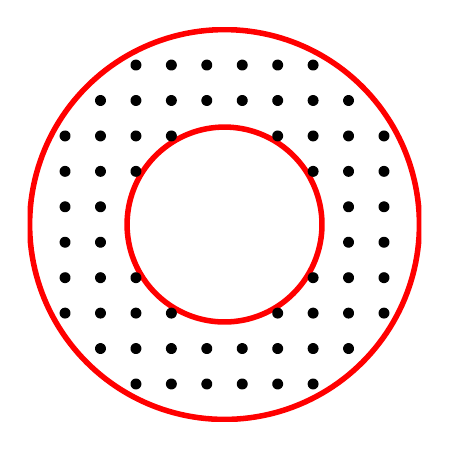
\begin{tikzpicture}

\begin{axis}[%
hide axis,
width=5cm,
height=5cm,
at={(0cm,0cm)},
scale only axis,
xmin=-10.1,
xmax=10.1,
ymin=-10.1,
ymax=10.1,
axis background/.style={fill=white},
]
\addplot [color=red, line width=2.0pt, forget plot]
  table[row sep=crcr]{%
10	0\\
9.99464587476366	-0.327190828217761\\
9.97858923238604	-0.654031292301431\\
9.95184726672197	-0.980171403295606\\
9.9144486137381	-1.30526192220052\\
9.86643332084879	-1.62895473394589\\
9.8078528040323	-1.95090322016128\\
9.73876979277334	-2.27076263034373\\
9.65925826289068	-2.58819045102521\\
9.56940335732209	-2.90284677254462\\
9.46930129495106	-3.21439465303162\\
9.35905926757326	-3.52250047921233\\
9.23879532511287	-3.8268343236509\\
9.10863824921176	-4.12707029804395\\
8.96872741532688	-4.42288690219001\\
8.81921264348355	-4.71396736825998\\
8.66025403784439	-5\\
8.49202181526579	-5.28067850650368\\
8.31469612302545	-5.55570233019602\\
8.12846684591615	-5.82477696867802\\
7.93353340291235	-6.08761429008721\\
7.73010453362737	-6.34393284163646\\
7.51839807478977	-6.59345815100069\\
7.29864072697836	-6.83592302022871\\
7.07106781186548	-7.07106781186547\\
6.83592302022871	-7.29864072697836\\
6.59345815100069	-7.51839807478977\\
6.34393284163646	-7.73010453362737\\
6.08761429008721	-7.93353340291235\\
5.82477696867802	-8.12846684591615\\
5.55570233019602	-8.31469612302545\\
5.28067850650368	-8.49202181526579\\
5	-8.66025403784439\\
4.71396736825998	-8.81921264348355\\
4.42288690219001	-8.96872741532688\\
4.12707029804395	-9.10863824921176\\
3.8268343236509	-9.23879532511287\\
3.52250047921234	-9.35905926757326\\
3.21439465303162	-9.46930129495106\\
2.90284677254462	-9.56940335732209\\
2.58819045102521	-9.65925826289068\\
2.27076263034373	-9.73876979277334\\
1.95090322016128	-9.8078528040323\\
1.62895473394589	-9.86643332084879\\
1.30526192220052	-9.9144486137381\\
0.980171403295605	-9.95184726672197\\
0.654031292301433	-9.97858923238604\\
0.327190828217762	-9.99464587476366\\
6.12323399573677e-16	-10\\
-0.32719082821776	-9.99464587476366\\
-0.654031292301431	-9.97858923238604\\
-0.980171403295604	-9.95184726672197\\
-1.30526192220052	-9.9144486137381\\
-1.62895473394589	-9.86643332084879\\
-1.95090322016128	-9.8078528040323\\
-2.27076263034373	-9.73876979277334\\
-2.58819045102521	-9.65925826289068\\
-2.90284677254462	-9.56940335732209\\
-3.21439465303162	-9.46930129495106\\
-3.52250047921233	-9.35905926757326\\
-3.8268343236509	-9.23879532511287\\
-4.12707029804395	-9.10863824921176\\
-4.42288690219001	-8.96872741532688\\
-4.71396736825998	-8.81921264348355\\
-5	-8.66025403784439\\
-5.28067850650368	-8.49202181526579\\
-5.55570233019602	-8.31469612302545\\
-5.82477696867802	-8.12846684591615\\
-6.08761429008721	-7.93353340291235\\
-6.34393284163645	-7.73010453362737\\
-6.59345815100069	-7.51839807478977\\
-6.83592302022871	-7.29864072697835\\
-7.07106781186547	-7.07106781186548\\
-7.29864072697835	-6.83592302022872\\
-7.51839807478977	-6.59345815100069\\
-7.73010453362737	-6.34393284163646\\
-7.93353340291235	-6.08761429008721\\
-8.12846684591615	-5.82477696867802\\
-8.31469612302545	-5.55570233019603\\
-8.49202181526579	-5.28067850650368\\
-8.66025403784439	-5\\
-8.81921264348355	-4.71396736825998\\
-8.96872741532688	-4.42288690219002\\
-9.10863824921176	-4.12707029804395\\
-9.23879532511287	-3.8268343236509\\
-9.35905926757326	-3.52250047921233\\
-9.46930129495106	-3.21439465303162\\
-9.56940335732209	-2.90284677254463\\
-9.65925826289068	-2.58819045102521\\
-9.73876979277334	-2.27076263034373\\
-9.8078528040323	-1.95090322016128\\
-9.86643332084879	-1.62895473394589\\
-9.9144486137381	-1.30526192220052\\
-9.95184726672197	-0.980171403295608\\
-9.97858923238604	-0.654031292301431\\
-9.99464587476366	-0.32719082821776\\
-10	-1.22464679914735e-15\\
-9.99464587476366	0.327190828217758\\
-9.97858923238604	0.654031292301429\\
-9.95184726672197	0.980171403295606\\
-9.9144486137381	1.30526192220052\\
-9.86643332084879	1.62895473394589\\
-9.80785280403231	1.95090322016128\\
-9.73876979277334	2.27076263034373\\
-9.65925826289068	2.58819045102521\\
-9.56940335732209	2.90284677254463\\
-9.46930129495106	3.21439465303162\\
-9.35905926757326	3.52250047921233\\
-9.23879532511287	3.8268343236509\\
-9.10863824921176	4.12707029804394\\
-8.96872741532688	4.42288690219001\\
-8.81921264348355	4.71396736825998\\
-8.66025403784439	5\\
-8.49202181526579	5.28067850650368\\
-8.31469612302545	5.55570233019602\\
-8.12846684591615	5.82477696867802\\
-7.93353340291235	6.08761429008721\\
-7.73010453362737	6.34393284163645\\
-7.51839807478977	6.59345815100069\\
-7.29864072697836	6.83592302022871\\
-7.07106781186548	7.07106781186547\\
-6.83592302022871	7.29864072697836\\
-6.59345815100069	7.51839807478977\\
-6.34393284163646	7.73010453362737\\
-6.08761429008721	7.93353340291235\\
-5.82477696867802	8.12846684591615\\
-5.55570233019602	8.31469612302545\\
-5.28067850650368	8.49202181526579\\
-5	8.66025403784439\\
-4.71396736825998	8.81921264348355\\
-4.42288690219001	8.96872741532688\\
-4.12707029804395	9.10863824921176\\
-3.8268343236509	9.23879532511287\\
-3.52250047921234	9.35905926757325\\
-3.21439465303162	9.46930129495106\\
-2.90284677254462	9.56940335732209\\
-2.58819045102521	9.65925826289068\\
-2.27076263034373	9.73876979277334\\
-1.95090322016129	9.8078528040323\\
-1.62895473394589	9.86643332084879\\
-1.30526192220052	9.9144486137381\\
-0.980171403295613	9.95184726672197\\
-0.654031292301427	9.97858923238604\\
-0.327190828217765	9.99464587476366\\
-1.83697019872103e-15	10\\
0.327190828217761	9.99464587476366\\
0.654031292301424	9.97858923238604\\
0.98017140329561	9.95184726672197\\
1.30526192220051	9.91444861373811\\
1.62895473394589	9.86643332084879\\
1.95090322016128	9.8078528040323\\
2.27076263034373	9.73876979277334\\
2.5881904510252	9.65925826289068\\
2.90284677254462	9.56940335732209\\
3.21439465303161	9.46930129495106\\
3.52250047921234	9.35905926757326\\
3.82683432365089	9.23879532511287\\
4.12707029804394	9.10863824921176\\
4.42288690219001	8.96872741532689\\
4.71396736825998	8.81921264348355\\
5	8.66025403784439\\
5.28067850650367	8.49202181526579\\
5.55570233019602	8.31469612302545\\
5.82477696867802	8.12846684591615\\
6.0876142900872	7.93353340291236\\
6.34393284163645	7.73010453362737\\
6.59345815100069	7.51839807478977\\
6.83592302022872	7.29864072697835\\
7.07106781186547	7.07106781186548\\
7.29864072697836	6.83592302022871\\
7.51839807478977	6.59345815100069\\
7.73010453362737	6.34393284163646\\
7.93353340291235	6.08761429008721\\
8.12846684591615	5.82477696867802\\
8.31469612302545	5.55570233019603\\
8.49202181526578	5.28067850650369\\
8.66025403784438	5\\
8.81921264348355	4.71396736825997\\
8.96872741532688	4.42288690219001\\
9.10863824921176	4.12707029804395\\
9.23879532511287	3.8268343236509\\
9.35905926757325	3.52250047921234\\
9.46930129495106	3.21439465303162\\
9.56940335732209	2.90284677254462\\
9.65925826289068	2.58819045102522\\
9.73876979277333	2.27076263034374\\
9.8078528040323	1.95090322016129\\
9.86643332084879	1.62895473394588\\
9.9144486137381	1.30526192220052\\
9.95184726672197	0.980171403295605\\
9.97858923238604	0.654031292301428\\
9.99464587476366	0.327190828217766\\
10	0\\
};
\addplot [color=red, line width=2.0pt, forget plot]
  table[row sep=crcr]{%
5	0\\
4.99732293738183	0.163595414108881\\
4.98929461619302	0.327015646150715\\
4.97592363336098	0.490085701647803\\
4.95722430686905	0.652630961100258\\
4.93321666042439	0.814477366972944\\
4.90392640201615	0.975451610080641\\
4.86938489638667	1.13538131517187\\
4.82962913144534	1.2940952255126\\
4.78470167866104	1.45142338627231\\
4.73465064747553	1.60719732651581\\
4.67952963378663	1.76125023960617\\
4.61939766255643	1.91341716182545\\
4.55431912460588	2.06353514902197\\
4.48436370766344	2.21144345109501\\
4.40960632174178	2.35698368412999\\
4.33012701892219	2.5\\
4.24601090763289	2.64033925325184\\
4.15734806151273	2.77785116509801\\
4.06423342295808	2.91238848433901\\
3.96676670145618	3.0438071450436\\
3.86505226681368	3.17196642081823\\
3.75919903739489	3.29672907550034\\
3.64932036348918	3.41796151011436\\
3.53553390593274	3.53553390593274\\
3.41796151011436	3.64932036348918\\
3.29672907550034	3.75919903739489\\
3.17196642081823	3.86505226681368\\
3.0438071450436	3.96676670145618\\
2.91238848433901	4.06423342295808\\
2.77785116509801	4.15734806151273\\
2.64033925325184	4.24601090763289\\
2.5	4.33012701892219\\
2.35698368412999	4.40960632174178\\
2.21144345109501	4.48436370766344\\
2.06353514902197	4.55431912460588\\
1.91341716182545	4.61939766255643\\
1.76125023960617	4.67952963378663\\
1.60719732651581	4.73465064747553\\
1.45142338627231	4.78470167866104\\
1.2940952255126	4.82962913144534\\
1.13538131517187	4.86938489638667\\
0.975451610080642	4.90392640201615\\
0.814477366972944	4.93321666042439\\
0.652630961100259	4.95722430686905\\
0.490085701647803	4.97592363336098\\
0.327015646150716	4.98929461619302\\
0.163595414108881	4.99732293738183\\
3.06161699786838e-16	5\\
-0.16359541410888	4.99732293738183\\
-0.327015646150716	4.98929461619302\\
-0.490085701647802	4.97592363336098\\
-0.652630961100258	4.95722430686905\\
-0.814477366972943	4.93321666042439\\
-0.975451610080641	4.90392640201615\\
-1.13538131517187	4.86938489638667\\
-1.2940952255126	4.82962913144534\\
-1.45142338627231	4.78470167866104\\
-1.60719732651581	4.73465064747553\\
-1.76125023960617	4.67952963378663\\
-1.91341716182545	4.61939766255643\\
-2.06353514902197	4.55431912460588\\
-2.21144345109501	4.48436370766344\\
-2.35698368412999	4.40960632174178\\
-2.5	4.33012701892219\\
-2.64033925325184	4.24601090763289\\
-2.77785116509801	4.15734806151273\\
-2.91238848433901	4.06423342295808\\
-3.0438071450436	3.96676670145618\\
-3.17196642081823	3.86505226681369\\
-3.29672907550034	3.75919903739489\\
-3.41796151011436	3.64932036348918\\
-3.53553390593274	3.53553390593274\\
-3.64932036348918	3.41796151011436\\
-3.75919903739489	3.29672907550034\\
-3.86505226681368	3.17196642081823\\
-3.96676670145618	3.0438071450436\\
-4.06423342295808	2.91238848433901\\
-4.15734806151273	2.77785116509801\\
-4.24601090763289	2.64033925325184\\
-4.33012701892219	2.5\\
-4.40960632174177	2.35698368412999\\
-4.48436370766344	2.21144345109501\\
-4.55431912460588	2.06353514902197\\
-4.61939766255643	1.91341716182545\\
-4.67952963378663	1.76125023960617\\
-4.73465064747553	1.60719732651581\\
-4.78470167866104	1.45142338627231\\
-4.82962913144534	1.29409522551261\\
-4.86938489638667	1.13538131517187\\
-4.90392640201615	0.975451610080641\\
-4.93321666042439	0.814477366972944\\
-4.95722430686905	0.65263096110026\\
-4.97592363336098	0.490085701647804\\
-4.98929461619302	0.327015646150716\\
-4.99732293738183	0.16359541410888\\
-5	6.12323399573677e-16\\
-4.99732293738183	-0.163595414108879\\
-4.98929461619302	-0.327015646150714\\
-4.97592363336098	-0.490085701647803\\
-4.95722430686905	-0.652630961100259\\
-4.93321666042439	-0.814477366972943\\
-4.90392640201615	-0.97545161008064\\
-4.86938489638667	-1.13538131517187\\
-4.82962913144534	-1.2940952255126\\
-4.78470167866104	-1.45142338627231\\
-4.73465064747553	-1.60719732651581\\
-4.67952963378663	-1.76125023960617\\
-4.61939766255643	-1.91341716182545\\
-4.55431912460588	-2.06353514902197\\
-4.48436370766344	-2.21144345109501\\
-4.40960632174178	-2.35698368412999\\
-4.33012701892219	-2.5\\
-4.2460109076329	-2.64033925325184\\
-4.15734806151273	-2.77785116509801\\
-4.06423342295808	-2.91238848433901\\
-3.96676670145618	-3.0438071450436\\
-3.86505226681369	-3.17196642081823\\
-3.75919903739489	-3.29672907550034\\
-3.64932036348918	-3.41796151011436\\
-3.53553390593274	-3.53553390593274\\
-3.41796151011436	-3.64932036348918\\
-3.29672907550035	-3.75919903739489\\
-3.17196642081823	-3.86505226681368\\
-3.0438071450436	-3.96676670145617\\
-2.91238848433901	-4.06423342295808\\
-2.77785116509801	-4.15734806151273\\
-2.64033925325184	-4.2460109076329\\
-2.5	-4.33012701892219\\
-2.35698368412999	-4.40960632174177\\
-2.21144345109501	-4.48436370766344\\
-2.06353514902197	-4.55431912460588\\
-1.91341716182545	-4.61939766255643\\
-1.76125023960617	-4.67952963378663\\
-1.60719732651581	-4.73465064747553\\
-1.45142338627231	-4.78470167866104\\
-1.2940952255126	-4.82962913144534\\
-1.13538131517186	-4.86938489638667\\
-0.975451610080643	-4.90392640201615\\
-0.814477366972945	-4.93321666042439\\
-0.652630961100258	-4.95722430686905\\
-0.490085701647807	-4.97592363336098\\
-0.327015646150714	-4.98929461619302\\
-0.163595414108883	-4.99732293738183\\
-9.18485099360515e-16	-5\\
0.163595414108881	-4.99732293738183\\
0.327015646150712	-4.98929461619302\\
0.490085701647805	-4.97592363336098\\
0.652630961100256	-4.95722430686905\\
0.814477366972943	-4.93321666042439\\
0.975451610080642	-4.90392640201615\\
1.13538131517186	-4.86938489638667\\
1.2940952255126	-4.82962913144534\\
1.45142338627231	-4.78470167866104\\
1.60719732651581	-4.73465064747553\\
1.76125023960617	-4.67952963378663\\
1.91341716182545	-4.61939766255643\\
2.06353514902197	-4.55431912460588\\
2.211443451095	-4.48436370766344\\
2.35698368412999	-4.40960632174178\\
2.5	-4.33012701892219\\
2.64033925325184	-4.2460109076329\\
2.77785116509801	-4.15734806151273\\
2.91238848433901	-4.06423342295808\\
3.0438071450436	-3.96676670145618\\
3.17196642081822	-3.86505226681369\\
3.29672907550035	-3.75919903739489\\
3.41796151011436	-3.64932036348918\\
3.53553390593274	-3.53553390593274\\
3.64932036348918	-3.41796151011436\\
3.75919903739489	-3.29672907550034\\
3.86505226681368	-3.17196642081823\\
3.96676670145617	-3.0438071450436\\
4.06423342295808	-2.91238848433901\\
4.15734806151272	-2.77785116509801\\
4.24601090763289	-2.64033925325184\\
4.33012701892219	-2.5\\
4.40960632174178	-2.35698368412999\\
4.48436370766344	-2.21144345109501\\
4.55431912460588	-2.06353514902197\\
4.61939766255643	-1.91341716182545\\
4.67952963378663	-1.76125023960617\\
4.73465064747553	-1.60719732651581\\
4.78470167866104	-1.45142338627231\\
4.82962913144534	-1.29409522551261\\
4.86938489638667	-1.13538131517187\\
4.90392640201615	-0.975451610080644\\
4.9332166604244	-0.814477366972941\\
4.95722430686905	-0.652630961100258\\
4.97592363336098	-0.490085701647803\\
4.98929461619302	-0.327015646150714\\
4.99732293738183	-0.163595414108883\\
5	0\\
};

\addplot[area legend, draw=black, fill=black, forget plot]
table[row sep=crcr] {%
x	y\\
-4.29545454545455	-8.18181818181818\\
-4.30025822535374	-8.13304560131415\\
-4.31448466232672	-8.08614732372691\\
-4.33758714237891	-8.04292562356328\\
-4.36867785015791	-8.00504148652155\\
-4.40656198719965	-7.97395077874255\\
-4.44978368736327	-7.95084829869036\\
-4.49668196495051	-7.93662186171737\\
-4.54545454545455	-7.93181818181818\\
-4.59422712595858	-7.93662186171737\\
-4.64112540354582	-7.95084829869036\\
-4.68434710370945	-7.97395077874255\\
-4.72223124075118	-8.00504148652155\\
-4.75332194853018	-8.04292562356328\\
-4.77642442858237	-8.08614732372691\\
-4.79065086555535	-8.13304560131415\\
-4.79545454545455	-8.18181818181818\\
-4.79065086555535	-8.23059076232221\\
-4.77642442858237	-8.27748903990945\\
-4.75332194853018	-8.32071074007308\\
-4.72223124075118	-8.35859487711482\\
-4.68434710370945	-8.38968558489382\\
-4.64112540354582	-8.412788064946\\
-4.59422712595858	-8.42701450191899\\
-4.54545454545455	-8.43181818181818\\
-4.49668196495051	-8.42701450191899\\
-4.44978368736327	-8.412788064946\\
-4.40656198719965	-8.38968558489382\\
-4.36867785015791	-8.35859487711482\\
-4.33758714237891	-8.32071074007308\\
-4.31448466232672	-8.27748903990945\\
-4.30025822535374	-8.23059076232221\\
-4.29545454545455	-8.18181818181818\\
}--cycle;

\addplot[area legend, draw=black, fill=black, forget plot]
table[row sep=crcr] {%
x	y\\
-2.47727272727273	-8.18181818181818\\
-2.48207640717192	-8.13304560131415\\
-2.49630284414491	-8.08614732372691\\
-2.51940532419709	-8.04292562356328\\
-2.55049603197609	-8.00504148652155\\
-2.58838016901783	-7.97395077874255\\
-2.63160186918146	-7.95084829869036\\
-2.6785001467687	-7.93662186171737\\
-2.72727272727273	-7.93181818181818\\
-2.77604530777676	-7.93662186171737\\
-2.822943585364	-7.95084829869036\\
-2.86616528552763	-7.97395077874255\\
-2.90404942256936	-8.00504148652155\\
-2.93514013034836	-8.04292562356328\\
-2.95824261040055	-8.08614732372691\\
-2.97246904737354	-8.13304560131415\\
-2.97727272727273	-8.18181818181818\\
-2.97246904737354	-8.23059076232221\\
-2.95824261040055	-8.27748903990945\\
-2.93514013034836	-8.32071074007308\\
-2.90404942256936	-8.35859487711482\\
-2.86616528552763	-8.38968558489382\\
-2.822943585364	-8.412788064946\\
-2.77604530777676	-8.42701450191899\\
-2.72727272727273	-8.43181818181818\\
-2.6785001467687	-8.42701450191899\\
-2.63160186918146	-8.412788064946\\
-2.58838016901783	-8.38968558489382\\
-2.55049603197609	-8.35859487711482\\
-2.51940532419709	-8.32071074007308\\
-2.49630284414491	-8.27748903990945\\
-2.48207640717192	-8.23059076232221\\
-2.47727272727273	-8.18181818181818\\
}--cycle;

\addplot[area legend, draw=black, fill=black, forget plot]
table[row sep=crcr] {%
x	y\\
-0.659090909090908	-8.18181818181818\\
-0.663894588990101	-8.13304560131415\\
-0.678121025963087	-8.08614732372691\\
-0.701223506015272	-8.04292562356328\\
-0.732314213794271	-8.00504148652155\\
-0.770198350836008	-7.97395077874255\\
-0.813420050999636	-7.95084829869036\\
-0.860318328586876	-7.93662186171737\\
-0.909090909090908	-7.93181818181818\\
-0.95786348959494	-7.93662186171737\\
-1.00476176718218	-7.95084829869036\\
-1.04798346734581	-7.97395077874255\\
-1.08586760438755	-8.00504148652155\\
-1.11695831216654	-8.04292562356328\\
-1.14006079221873	-8.08614732372691\\
-1.15428722919172	-8.13304560131415\\
-1.15909090909091	-8.18181818181818\\
-1.15428722919172	-8.23059076232221\\
-1.14006079221873	-8.27748903990945\\
-1.11695831216654	-8.32071074007308\\
-1.08586760438755	-8.35859487711482\\
-1.04798346734581	-8.38968558489382\\
-1.00476176718218	-8.412788064946\\
-0.95786348959494	-8.42701450191899\\
-0.909090909090908	-8.43181818181818\\
-0.860318328586876	-8.42701450191899\\
-0.813420050999636	-8.412788064946\\
-0.770198350836008	-8.38968558489382\\
-0.732314213794271	-8.35859487711482\\
-0.701223506015272	-8.32071074007308\\
-0.678121025963087	-8.27748903990945\\
-0.663894588990101	-8.23059076232221\\
-0.659090909090908	-8.18181818181818\\
}--cycle;

\addplot[area legend, draw=black, fill=black, forget plot]
table[row sep=crcr] {%
x	y\\
1.15909090909091	-8.18181818181818\\
1.15428722919172	-8.13304560131415\\
1.14006079221873	-8.08614732372691\\
1.11695831216654	-8.04292562356328\\
1.08586760438755	-8.00504148652155\\
1.04798346734581	-7.97395077874255\\
1.00476176718218	-7.95084829869036\\
0.95786348959494	-7.93662186171737\\
0.909090909090908	-7.93181818181818\\
0.860318328586876	-7.93662186171737\\
0.813420050999636	-7.95084829869036\\
0.770198350836008	-7.97395077874255\\
0.732314213794271	-8.00504148652155\\
0.701223506015272	-8.04292562356328\\
0.678121025963087	-8.08614732372691\\
0.663894588990101	-8.13304560131415\\
0.659090909090908	-8.18181818181818\\
0.663894588990101	-8.23059076232221\\
0.678121025963087	-8.27748903990945\\
0.701223506015272	-8.32071074007308\\
0.732314213794271	-8.35859487711482\\
0.770198350836008	-8.38968558489382\\
0.813420050999636	-8.412788064946\\
0.860318328586876	-8.42701450191899\\
0.909090909090908	-8.43181818181818\\
0.95786348959494	-8.42701450191899\\
1.00476176718218	-8.412788064946\\
1.04798346734581	-8.38968558489382\\
1.08586760438755	-8.35859487711482\\
1.11695831216654	-8.32071074007308\\
1.14006079221873	-8.27748903990945\\
1.15428722919172	-8.23059076232221\\
1.15909090909091	-8.18181818181818\\
}--cycle;

\addplot[area legend, draw=black, fill=black, forget plot]
table[row sep=crcr] {%
x	y\\
2.97727272727273	-8.18181818181818\\
2.97246904737353	-8.13304560131415\\
2.95824261040055	-8.08614732372691\\
2.93514013034836	-8.04292562356328\\
2.90404942256936	-8.00504148652155\\
2.86616528552763	-7.97395077874255\\
2.822943585364	-7.95084829869036\\
2.77604530777676	-7.93662186171737\\
2.72727272727273	-7.93181818181818\\
2.67850014676869	-7.93662186171737\\
2.63160186918145	-7.95084829869036\\
2.58838016901783	-7.97395077874255\\
2.55049603197609	-8.00504148652155\\
2.51940532419709	-8.04292562356328\\
2.49630284414491	-8.08614732372691\\
2.48207640717192	-8.13304560131415\\
2.47727272727273	-8.18181818181818\\
2.48207640717192	-8.23059076232221\\
2.49630284414491	-8.27748903990945\\
2.51940532419709	-8.32071074007308\\
2.55049603197609	-8.35859487711482\\
2.58838016901783	-8.38968558489382\\
2.63160186918145	-8.412788064946\\
2.67850014676869	-8.42701450191899\\
2.72727272727273	-8.43181818181818\\
2.77604530777676	-8.42701450191899\\
2.822943585364	-8.412788064946\\
2.86616528552763	-8.38968558489382\\
2.90404942256936	-8.35859487711482\\
2.93514013034836	-8.32071074007308\\
2.95824261040055	-8.27748903990945\\
2.97246904737353	-8.23059076232221\\
2.97727272727273	-8.18181818181818\\
}--cycle;

\addplot[area legend, draw=black, fill=black, forget plot]
table[row sep=crcr] {%
x	y\\
4.79545454545454	-8.18181818181818\\
4.79065086555535	-8.13304560131415\\
4.77642442858237	-8.08614732372691\\
4.75332194853018	-8.04292562356328\\
4.72223124075118	-8.00504148652155\\
4.68434710370945	-7.97395077874255\\
4.64112540354582	-7.95084829869036\\
4.59422712595858	-7.93662186171737\\
4.54545454545454	-7.93181818181818\\
4.49668196495051	-7.93662186171737\\
4.44978368736327	-7.95084829869036\\
4.40656198719964	-7.97395077874255\\
4.36867785015791	-8.00504148652155\\
4.33758714237891	-8.04292562356328\\
4.31448466232672	-8.08614732372691\\
4.30025822535374	-8.13304560131415\\
4.29545454545454	-8.18181818181818\\
4.30025822535374	-8.23059076232221\\
4.31448466232672	-8.27748903990945\\
4.33758714237891	-8.32071074007308\\
4.36867785015791	-8.35859487711482\\
4.40656198719964	-8.38968558489382\\
4.44978368736327	-8.412788064946\\
4.49668196495051	-8.42701450191899\\
4.54545454545454	-8.43181818181818\\
4.59422712595858	-8.42701450191899\\
4.64112540354582	-8.412788064946\\
4.68434710370945	-8.38968558489382\\
4.72223124075118	-8.35859487711482\\
4.75332194853018	-8.32071074007308\\
4.77642442858237	-8.27748903990945\\
4.79065086555535	-8.23059076232221\\
4.79545454545454	-8.18181818181818\\
}--cycle;

\addplot[area legend, draw=black, fill=black, forget plot]
table[row sep=crcr] {%
x	y\\
-6.11363636363636	-6.36363636363636\\
-6.11844004353556	-6.31486378313233\\
-6.13266648050854	-6.26796550554509\\
-6.15576896056073	-6.22474380538146\\
-6.18685966833973	-6.18685966833973\\
-6.22474380538146	-6.15576896056073\\
-6.26796550554509	-6.13266648050854\\
-6.31486378313233	-6.11844004353556\\
-6.36363636363636	-6.11363636363636\\
-6.4124089441404	-6.11844004353556\\
-6.45930722172764	-6.13266648050854\\
-6.50252892189126	-6.15576896056073\\
-6.540413058933	-6.18685966833973\\
-6.571503766712	-6.22474380538146\\
-6.59460624676418	-6.26796550554509\\
-6.60883268373717	-6.31486378313233\\
-6.61363636363636	-6.36363636363636\\
-6.60883268373717	-6.4124089441404\\
-6.59460624676418	-6.45930722172764\\
-6.571503766712	-6.50252892189126\\
-6.540413058933	-6.540413058933\\
-6.50252892189126	-6.571503766712\\
-6.45930722172764	-6.59460624676418\\
-6.4124089441404	-6.60883268373717\\
-6.36363636363636	-6.61363636363636\\
-6.31486378313233	-6.60883268373717\\
-6.26796550554509	-6.59460624676418\\
-6.22474380538146	-6.571503766712\\
-6.18685966833973	-6.540413058933\\
-6.15576896056073	-6.50252892189126\\
-6.13266648050854	-6.45930722172764\\
-6.11844004353556	-6.4124089441404\\
-6.11363636363636	-6.36363636363636\\
}--cycle;

\addplot[area legend, draw=black, fill=black, forget plot]
table[row sep=crcr] {%
x	y\\
-4.29545454545455	-6.36363636363636\\
-4.30025822535374	-6.31486378313233\\
-4.31448466232672	-6.26796550554509\\
-4.33758714237891	-6.22474380538146\\
-4.36867785015791	-6.18685966833973\\
-4.40656198719965	-6.15576896056073\\
-4.44978368736327	-6.13266648050854\\
-4.49668196495051	-6.11844004353556\\
-4.54545454545455	-6.11363636363636\\
-4.59422712595858	-6.11844004353556\\
-4.64112540354582	-6.13266648050854\\
-4.68434710370945	-6.15576896056073\\
-4.72223124075118	-6.18685966833973\\
-4.75332194853018	-6.22474380538146\\
-4.77642442858237	-6.26796550554509\\
-4.79065086555535	-6.31486378313233\\
-4.79545454545455	-6.36363636363636\\
-4.79065086555535	-6.4124089441404\\
-4.77642442858237	-6.45930722172764\\
-4.75332194853018	-6.50252892189126\\
-4.72223124075118	-6.540413058933\\
-4.68434710370945	-6.571503766712\\
-4.64112540354582	-6.59460624676418\\
-4.59422712595858	-6.60883268373717\\
-4.54545454545455	-6.61363636363636\\
-4.49668196495051	-6.60883268373717\\
-4.44978368736327	-6.59460624676418\\
-4.40656198719965	-6.571503766712\\
-4.36867785015791	-6.540413058933\\
-4.33758714237891	-6.50252892189126\\
-4.31448466232672	-6.45930722172764\\
-4.30025822535374	-6.4124089441404\\
-4.29545454545455	-6.36363636363636\\
}--cycle;

\addplot[area legend, draw=black, fill=black, forget plot]
table[row sep=crcr] {%
x	y\\
-2.47727272727273	-6.36363636363636\\
-2.48207640717192	-6.31486378313233\\
-2.49630284414491	-6.26796550554509\\
-2.51940532419709	-6.22474380538146\\
-2.55049603197609	-6.18685966833973\\
-2.58838016901783	-6.15576896056073\\
-2.63160186918146	-6.13266648050854\\
-2.6785001467687	-6.11844004353556\\
-2.72727272727273	-6.11363636363636\\
-2.77604530777676	-6.11844004353556\\
-2.822943585364	-6.13266648050854\\
-2.86616528552763	-6.15576896056073\\
-2.90404942256936	-6.18685966833973\\
-2.93514013034836	-6.22474380538146\\
-2.95824261040055	-6.26796550554509\\
-2.97246904737354	-6.31486378313233\\
-2.97727272727273	-6.36363636363636\\
-2.97246904737354	-6.4124089441404\\
-2.95824261040055	-6.45930722172764\\
-2.93514013034836	-6.50252892189126\\
-2.90404942256936	-6.540413058933\\
-2.86616528552763	-6.571503766712\\
-2.822943585364	-6.59460624676418\\
-2.77604530777676	-6.60883268373717\\
-2.72727272727273	-6.61363636363636\\
-2.6785001467687	-6.60883268373717\\
-2.63160186918146	-6.59460624676418\\
-2.58838016901783	-6.571503766712\\
-2.55049603197609	-6.540413058933\\
-2.51940532419709	-6.50252892189126\\
-2.49630284414491	-6.45930722172764\\
-2.48207640717192	-6.4124089441404\\
-2.47727272727273	-6.36363636363636\\
}--cycle;

\addplot[area legend, draw=black, fill=black, forget plot]
table[row sep=crcr] {%
x	y\\
-0.659090909090908	-6.36363636363636\\
-0.663894588990101	-6.31486378313233\\
-0.678121025963087	-6.26796550554509\\
-0.701223506015272	-6.22474380538146\\
-0.732314213794271	-6.18685966833973\\
-0.770198350836008	-6.15576896056073\\
-0.813420050999636	-6.13266648050854\\
-0.860318328586876	-6.11844004353556\\
-0.909090909090908	-6.11363636363636\\
-0.95786348959494	-6.11844004353556\\
-1.00476176718218	-6.13266648050854\\
-1.04798346734581	-6.15576896056073\\
-1.08586760438755	-6.18685966833973\\
-1.11695831216654	-6.22474380538146\\
-1.14006079221873	-6.26796550554509\\
-1.15428722919172	-6.31486378313233\\
-1.15909090909091	-6.36363636363636\\
-1.15428722919172	-6.4124089441404\\
-1.14006079221873	-6.45930722172764\\
-1.11695831216654	-6.50252892189126\\
-1.08586760438755	-6.540413058933\\
-1.04798346734581	-6.571503766712\\
-1.00476176718218	-6.59460624676418\\
-0.95786348959494	-6.60883268373717\\
-0.909090909090908	-6.61363636363636\\
-0.860318328586876	-6.60883268373717\\
-0.813420050999636	-6.59460624676418\\
-0.770198350836008	-6.571503766712\\
-0.732314213794271	-6.540413058933\\
-0.701223506015272	-6.50252892189126\\
-0.678121025963087	-6.45930722172764\\
-0.663894588990101	-6.4124089441404\\
-0.659090909090908	-6.36363636363636\\
}--cycle;

\addplot[area legend, draw=black, fill=black, forget plot]
table[row sep=crcr] {%
x	y\\
1.15909090909091	-6.36363636363636\\
1.15428722919172	-6.31486378313233\\
1.14006079221873	-6.26796550554509\\
1.11695831216654	-6.22474380538146\\
1.08586760438755	-6.18685966833973\\
1.04798346734581	-6.15576896056073\\
1.00476176718218	-6.13266648050854\\
0.95786348959494	-6.11844004353556\\
0.909090909090908	-6.11363636363636\\
0.860318328586876	-6.11844004353556\\
0.813420050999636	-6.13266648050854\\
0.770198350836008	-6.15576896056073\\
0.732314213794271	-6.18685966833973\\
0.701223506015272	-6.22474380538146\\
0.678121025963087	-6.26796550554509\\
0.663894588990101	-6.31486378313233\\
0.659090909090908	-6.36363636363636\\
0.663894588990101	-6.4124089441404\\
0.678121025963087	-6.45930722172764\\
0.701223506015272	-6.50252892189126\\
0.732314213794271	-6.540413058933\\
0.770198350836008	-6.571503766712\\
0.813420050999636	-6.59460624676418\\
0.860318328586876	-6.60883268373717\\
0.909090909090908	-6.61363636363636\\
0.95786348959494	-6.60883268373717\\
1.00476176718218	-6.59460624676418\\
1.04798346734581	-6.571503766712\\
1.08586760438755	-6.540413058933\\
1.11695831216654	-6.50252892189126\\
1.14006079221873	-6.45930722172764\\
1.15428722919172	-6.4124089441404\\
1.15909090909091	-6.36363636363636\\
}--cycle;

\addplot[area legend, draw=black, fill=black, forget plot]
table[row sep=crcr] {%
x	y\\
2.97727272727273	-6.36363636363636\\
2.97246904737353	-6.31486378313233\\
2.95824261040055	-6.26796550554509\\
2.93514013034836	-6.22474380538146\\
2.90404942256936	-6.18685966833973\\
2.86616528552763	-6.15576896056073\\
2.822943585364	-6.13266648050854\\
2.77604530777676	-6.11844004353556\\
2.72727272727273	-6.11363636363636\\
2.67850014676869	-6.11844004353556\\
2.63160186918145	-6.13266648050854\\
2.58838016901783	-6.15576896056073\\
2.55049603197609	-6.18685966833973\\
2.51940532419709	-6.22474380538146\\
2.49630284414491	-6.26796550554509\\
2.48207640717192	-6.31486378313233\\
2.47727272727273	-6.36363636363636\\
2.48207640717192	-6.4124089441404\\
2.49630284414491	-6.45930722172764\\
2.51940532419709	-6.50252892189126\\
2.55049603197609	-6.540413058933\\
2.58838016901783	-6.571503766712\\
2.63160186918145	-6.59460624676418\\
2.67850014676869	-6.60883268373717\\
2.72727272727273	-6.61363636363636\\
2.77604530777676	-6.60883268373717\\
2.822943585364	-6.59460624676418\\
2.86616528552763	-6.571503766712\\
2.90404942256936	-6.540413058933\\
2.93514013034836	-6.50252892189126\\
2.95824261040055	-6.45930722172764\\
2.97246904737353	-6.4124089441404\\
2.97727272727273	-6.36363636363636\\
}--cycle;

\addplot[area legend, draw=black, fill=black, forget plot]
table[row sep=crcr] {%
x	y\\
4.79545454545454	-6.36363636363636\\
4.79065086555535	-6.31486378313233\\
4.77642442858237	-6.26796550554509\\
4.75332194853018	-6.22474380538146\\
4.72223124075118	-6.18685966833973\\
4.68434710370945	-6.15576896056073\\
4.64112540354582	-6.13266648050854\\
4.59422712595858	-6.11844004353556\\
4.54545454545454	-6.11363636363636\\
4.49668196495051	-6.11844004353556\\
4.44978368736327	-6.13266648050854\\
4.40656198719964	-6.15576896056073\\
4.36867785015791	-6.18685966833973\\
4.33758714237891	-6.22474380538146\\
4.31448466232672	-6.26796550554509\\
4.30025822535374	-6.31486378313233\\
4.29545454545454	-6.36363636363636\\
4.30025822535374	-6.4124089441404\\
4.31448466232672	-6.45930722172764\\
4.33758714237891	-6.50252892189126\\
4.36867785015791	-6.540413058933\\
4.40656198719964	-6.571503766712\\
4.44978368736327	-6.59460624676418\\
4.49668196495051	-6.60883268373717\\
4.54545454545454	-6.61363636363636\\
4.59422712595858	-6.60883268373717\\
4.64112540354582	-6.59460624676418\\
4.68434710370945	-6.571503766712\\
4.72223124075118	-6.540413058933\\
4.75332194853018	-6.50252892189126\\
4.77642442858237	-6.45930722172764\\
4.79065086555535	-6.4124089441404\\
4.79545454545454	-6.36363636363636\\
}--cycle;

\addplot[area legend, draw=black, fill=black, forget plot]
table[row sep=crcr] {%
x	y\\
6.61363636363636	-6.36363636363636\\
6.60883268373717	-6.31486378313233\\
6.59460624676418	-6.26796550554509\\
6.571503766712	-6.22474380538146\\
6.540413058933	-6.18685966833973\\
6.50252892189126	-6.15576896056073\\
6.45930722172764	-6.13266648050854\\
6.4124089441404	-6.11844004353556\\
6.36363636363636	-6.11363636363636\\
6.31486378313233	-6.11844004353556\\
6.26796550554509	-6.13266648050854\\
6.22474380538146	-6.15576896056073\\
6.18685966833973	-6.18685966833973\\
6.15576896056073	-6.22474380538146\\
6.13266648050854	-6.26796550554509\\
6.11844004353556	-6.31486378313233\\
6.11363636363636	-6.36363636363636\\
6.11844004353556	-6.4124089441404\\
6.13266648050854	-6.45930722172764\\
6.15576896056073	-6.50252892189126\\
6.18685966833973	-6.540413058933\\
6.22474380538146	-6.571503766712\\
6.26796550554509	-6.59460624676418\\
6.31486378313233	-6.60883268373717\\
6.36363636363636	-6.61363636363636\\
6.4124089441404	-6.60883268373717\\
6.45930722172764	-6.59460624676418\\
6.50252892189126	-6.571503766712\\
6.540413058933	-6.540413058933\\
6.571503766712	-6.50252892189126\\
6.59460624676418	-6.45930722172764\\
6.60883268373717	-6.4124089441404\\
6.61363636363636	-6.36363636363636\\
}--cycle;

\addplot[area legend, draw=black, fill=black, forget plot]
table[row sep=crcr] {%
x	y\\
-7.93181818181818	-4.54545454545455\\
-7.93662186171737	-4.49668196495051\\
-7.95084829869036	-4.44978368736327\\
-7.97395077874255	-4.40656198719965\\
-8.00504148652155	-4.36867785015791\\
-8.04292562356328	-4.33758714237891\\
-8.08614732372691	-4.31448466232672\\
-8.13304560131415	-4.30025822535374\\
-8.18181818181818	-4.29545454545455\\
-8.23059076232221	-4.30025822535374\\
-8.27748903990945	-4.31448466232672\\
-8.32071074007308	-4.33758714237891\\
-8.35859487711482	-4.36867785015791\\
-8.38968558489382	-4.40656198719965\\
-8.412788064946	-4.44978368736327\\
-8.42701450191899	-4.49668196495051\\
-8.43181818181818	-4.54545454545455\\
-8.42701450191899	-4.59422712595858\\
-8.412788064946	-4.64112540354582\\
-8.38968558489382	-4.68434710370945\\
-8.35859487711482	-4.72223124075118\\
-8.32071074007308	-4.75332194853018\\
-8.27748903990945	-4.77642442858237\\
-8.23059076232221	-4.79065086555535\\
-8.18181818181818	-4.79545454545455\\
-8.13304560131415	-4.79065086555535\\
-8.08614732372691	-4.77642442858237\\
-8.04292562356328	-4.75332194853018\\
-8.00504148652155	-4.72223124075118\\
-7.97395077874255	-4.68434710370945\\
-7.95084829869036	-4.64112540354582\\
-7.93662186171737	-4.59422712595858\\
-7.93181818181818	-4.54545454545455\\
}--cycle;

\addplot[area legend, draw=black, fill=black, forget plot]
table[row sep=crcr] {%
x	y\\
-6.11363636363636	-4.54545454545455\\
-6.11844004353556	-4.49668196495051\\
-6.13266648050854	-4.44978368736327\\
-6.15576896056073	-4.40656198719965\\
-6.18685966833973	-4.36867785015791\\
-6.22474380538146	-4.33758714237891\\
-6.26796550554509	-4.31448466232672\\
-6.31486378313233	-4.30025822535374\\
-6.36363636363636	-4.29545454545455\\
-6.4124089441404	-4.30025822535374\\
-6.45930722172764	-4.31448466232672\\
-6.50252892189126	-4.33758714237891\\
-6.540413058933	-4.36867785015791\\
-6.571503766712	-4.40656198719965\\
-6.59460624676418	-4.44978368736327\\
-6.60883268373717	-4.49668196495051\\
-6.61363636363636	-4.54545454545455\\
-6.60883268373717	-4.59422712595858\\
-6.59460624676418	-4.64112540354582\\
-6.571503766712	-4.68434710370945\\
-6.540413058933	-4.72223124075118\\
-6.50252892189126	-4.75332194853018\\
-6.45930722172764	-4.77642442858237\\
-6.4124089441404	-4.79065086555535\\
-6.36363636363636	-4.79545454545455\\
-6.31486378313233	-4.79065086555535\\
-6.26796550554509	-4.77642442858237\\
-6.22474380538146	-4.75332194853018\\
-6.18685966833973	-4.72223124075118\\
-6.15576896056073	-4.68434710370945\\
-6.13266648050854	-4.64112540354582\\
-6.11844004353556	-4.59422712595858\\
-6.11363636363636	-4.54545454545455\\
}--cycle;

\addplot[area legend, draw=black, fill=black, forget plot]
table[row sep=crcr] {%
x	y\\
-4.29545454545455	-4.54545454545455\\
-4.30025822535374	-4.49668196495051\\
-4.31448466232672	-4.44978368736327\\
-4.33758714237891	-4.40656198719965\\
-4.36867785015791	-4.36867785015791\\
-4.40656198719965	-4.33758714237891\\
-4.44978368736327	-4.31448466232672\\
-4.49668196495051	-4.30025822535374\\
-4.54545454545455	-4.29545454545455\\
-4.59422712595858	-4.30025822535374\\
-4.64112540354582	-4.31448466232672\\
-4.68434710370945	-4.33758714237891\\
-4.72223124075118	-4.36867785015791\\
-4.75332194853018	-4.40656198719965\\
-4.77642442858237	-4.44978368736327\\
-4.79065086555535	-4.49668196495051\\
-4.79545454545455	-4.54545454545455\\
-4.79065086555535	-4.59422712595858\\
-4.77642442858237	-4.64112540354582\\
-4.75332194853018	-4.68434710370945\\
-4.72223124075118	-4.72223124075118\\
-4.68434710370945	-4.75332194853018\\
-4.64112540354582	-4.77642442858237\\
-4.59422712595858	-4.79065086555535\\
-4.54545454545455	-4.79545454545455\\
-4.49668196495051	-4.79065086555535\\
-4.44978368736327	-4.77642442858237\\
-4.40656198719965	-4.75332194853018\\
-4.36867785015791	-4.72223124075118\\
-4.33758714237891	-4.68434710370945\\
-4.31448466232672	-4.64112540354582\\
-4.30025822535374	-4.59422712595858\\
-4.29545454545455	-4.54545454545455\\
}--cycle;

\addplot[area legend, draw=black, fill=black, forget plot]
table[row sep=crcr] {%
x	y\\
-2.47727272727273	-4.54545454545455\\
-2.48207640717192	-4.49668196495051\\
-2.49630284414491	-4.44978368736327\\
-2.51940532419709	-4.40656198719965\\
-2.55049603197609	-4.36867785015791\\
-2.58838016901783	-4.33758714237891\\
-2.63160186918146	-4.31448466232672\\
-2.6785001467687	-4.30025822535374\\
-2.72727272727273	-4.29545454545455\\
-2.77604530777676	-4.30025822535374\\
-2.822943585364	-4.31448466232672\\
-2.86616528552763	-4.33758714237891\\
-2.90404942256936	-4.36867785015791\\
-2.93514013034836	-4.40656198719965\\
-2.95824261040055	-4.44978368736327\\
-2.97246904737354	-4.49668196495051\\
-2.97727272727273	-4.54545454545455\\
-2.97246904737354	-4.59422712595858\\
-2.95824261040055	-4.64112540354582\\
-2.93514013034836	-4.68434710370945\\
-2.90404942256936	-4.72223124075118\\
-2.86616528552763	-4.75332194853018\\
-2.822943585364	-4.77642442858237\\
-2.77604530777676	-4.79065086555535\\
-2.72727272727273	-4.79545454545455\\
-2.6785001467687	-4.79065086555535\\
-2.63160186918146	-4.77642442858237\\
-2.58838016901783	-4.75332194853018\\
-2.55049603197609	-4.72223124075118\\
-2.51940532419709	-4.68434710370945\\
-2.49630284414491	-4.64112540354582\\
-2.48207640717192	-4.59422712595858\\
-2.47727272727273	-4.54545454545455\\
}--cycle;

\addplot[area legend, draw=black, fill=black, forget plot]
table[row sep=crcr] {%
x	y\\
2.97727272727273	-4.54545454545455\\
2.97246904737353	-4.49668196495051\\
2.95824261040055	-4.44978368736327\\
2.93514013034836	-4.40656198719965\\
2.90404942256936	-4.36867785015791\\
2.86616528552763	-4.33758714237891\\
2.822943585364	-4.31448466232672\\
2.77604530777676	-4.30025822535374\\
2.72727272727273	-4.29545454545455\\
2.67850014676869	-4.30025822535374\\
2.63160186918145	-4.31448466232672\\
2.58838016901783	-4.33758714237891\\
2.55049603197609	-4.36867785015791\\
2.51940532419709	-4.40656198719965\\
2.49630284414491	-4.44978368736327\\
2.48207640717192	-4.49668196495051\\
2.47727272727273	-4.54545454545455\\
2.48207640717192	-4.59422712595858\\
2.49630284414491	-4.64112540354582\\
2.51940532419709	-4.68434710370945\\
2.55049603197609	-4.72223124075118\\
2.58838016901783	-4.75332194853018\\
2.63160186918145	-4.77642442858237\\
2.67850014676869	-4.79065086555535\\
2.72727272727273	-4.79545454545455\\
2.77604530777676	-4.79065086555535\\
2.822943585364	-4.77642442858237\\
2.86616528552763	-4.75332194853018\\
2.90404942256936	-4.72223124075118\\
2.93514013034836	-4.68434710370945\\
2.95824261040055	-4.64112540354582\\
2.97246904737353	-4.59422712595858\\
2.97727272727273	-4.54545454545455\\
}--cycle;

\addplot[area legend, draw=black, fill=black, forget plot]
table[row sep=crcr] {%
x	y\\
4.79545454545454	-4.54545454545455\\
4.79065086555535	-4.49668196495051\\
4.77642442858237	-4.44978368736327\\
4.75332194853018	-4.40656198719965\\
4.72223124075118	-4.36867785015791\\
4.68434710370945	-4.33758714237891\\
4.64112540354582	-4.31448466232672\\
4.59422712595858	-4.30025822535374\\
4.54545454545454	-4.29545454545455\\
4.49668196495051	-4.30025822535374\\
4.44978368736327	-4.31448466232672\\
4.40656198719964	-4.33758714237891\\
4.36867785015791	-4.36867785015791\\
4.33758714237891	-4.40656198719965\\
4.31448466232672	-4.44978368736327\\
4.30025822535374	-4.49668196495051\\
4.29545454545454	-4.54545454545455\\
4.30025822535374	-4.59422712595858\\
4.31448466232672	-4.64112540354582\\
4.33758714237891	-4.68434710370945\\
4.36867785015791	-4.72223124075118\\
4.40656198719964	-4.75332194853018\\
4.44978368736327	-4.77642442858237\\
4.49668196495051	-4.79065086555535\\
4.54545454545454	-4.79545454545455\\
4.59422712595858	-4.79065086555535\\
4.64112540354582	-4.77642442858237\\
4.68434710370945	-4.75332194853018\\
4.72223124075118	-4.72223124075118\\
4.75332194853018	-4.68434710370945\\
4.77642442858237	-4.64112540354582\\
4.79065086555535	-4.59422712595858\\
4.79545454545454	-4.54545454545455\\
}--cycle;

\addplot[area legend, draw=black, fill=black, forget plot]
table[row sep=crcr] {%
x	y\\
6.61363636363636	-4.54545454545455\\
6.60883268373717	-4.49668196495051\\
6.59460624676418	-4.44978368736327\\
6.571503766712	-4.40656198719965\\
6.540413058933	-4.36867785015791\\
6.50252892189126	-4.33758714237891\\
6.45930722172764	-4.31448466232672\\
6.4124089441404	-4.30025822535374\\
6.36363636363636	-4.29545454545455\\
6.31486378313233	-4.30025822535374\\
6.26796550554509	-4.31448466232672\\
6.22474380538146	-4.33758714237891\\
6.18685966833973	-4.36867785015791\\
6.15576896056073	-4.40656198719965\\
6.13266648050854	-4.44978368736327\\
6.11844004353556	-4.49668196495051\\
6.11363636363636	-4.54545454545455\\
6.11844004353556	-4.59422712595858\\
6.13266648050854	-4.64112540354582\\
6.15576896056073	-4.68434710370945\\
6.18685966833973	-4.72223124075118\\
6.22474380538146	-4.75332194853018\\
6.26796550554509	-4.77642442858237\\
6.31486378313233	-4.79065086555535\\
6.36363636363636	-4.79545454545455\\
6.4124089441404	-4.79065086555535\\
6.45930722172764	-4.77642442858237\\
6.50252892189126	-4.75332194853018\\
6.540413058933	-4.72223124075118\\
6.571503766712	-4.68434710370945\\
6.59460624676418	-4.64112540354582\\
6.60883268373717	-4.59422712595858\\
6.61363636363636	-4.54545454545455\\
}--cycle;

\addplot[area legend, draw=black, fill=black, forget plot]
table[row sep=crcr] {%
x	y\\
8.43181818181818	-4.54545454545455\\
8.42701450191899	-4.49668196495051\\
8.412788064946	-4.44978368736327\\
8.38968558489382	-4.40656198719965\\
8.35859487711482	-4.36867785015791\\
8.32071074007308	-4.33758714237891\\
8.27748903990946	-4.31448466232672\\
8.23059076232222	-4.30025822535374\\
8.18181818181818	-4.29545454545455\\
8.13304560131415	-4.30025822535374\\
8.08614732372691	-4.31448466232672\\
8.04292562356328	-4.33758714237891\\
8.00504148652155	-4.36867785015791\\
7.97395077874255	-4.40656198719965\\
7.95084829869036	-4.44978368736327\\
7.93662186171738	-4.49668196495051\\
7.93181818181818	-4.54545454545455\\
7.93662186171738	-4.59422712595858\\
7.95084829869036	-4.64112540354582\\
7.97395077874255	-4.68434710370945\\
8.00504148652155	-4.72223124075118\\
8.04292562356328	-4.75332194853018\\
8.08614732372691	-4.77642442858237\\
8.13304560131415	-4.79065086555535\\
8.18181818181818	-4.79545454545455\\
8.23059076232222	-4.79065086555535\\
8.27748903990946	-4.77642442858237\\
8.32071074007308	-4.75332194853018\\
8.35859487711482	-4.72223124075118\\
8.38968558489382	-4.68434710370945\\
8.412788064946	-4.64112540354582\\
8.42701450191899	-4.59422712595858\\
8.43181818181818	-4.54545454545455\\
}--cycle;

\addplot[area legend, draw=black, fill=black, forget plot]
table[row sep=crcr] {%
x	y\\
-7.93181818181818	-2.72727272727273\\
-7.93662186171737	-2.6785001467687\\
-7.95084829869036	-2.63160186918146\\
-7.97395077874255	-2.58838016901783\\
-8.00504148652155	-2.55049603197609\\
-8.04292562356328	-2.51940532419709\\
-8.08614732372691	-2.49630284414491\\
-8.13304560131415	-2.48207640717192\\
-8.18181818181818	-2.47727272727273\\
-8.23059076232221	-2.48207640717192\\
-8.27748903990945	-2.49630284414491\\
-8.32071074007308	-2.51940532419709\\
-8.35859487711482	-2.55049603197609\\
-8.38968558489382	-2.58838016901783\\
-8.412788064946	-2.63160186918146\\
-8.42701450191899	-2.6785001467687\\
-8.43181818181818	-2.72727272727273\\
-8.42701450191899	-2.77604530777676\\
-8.412788064946	-2.822943585364\\
-8.38968558489382	-2.86616528552763\\
-8.35859487711482	-2.90404942256936\\
-8.32071074007308	-2.93514013034836\\
-8.27748903990945	-2.95824261040055\\
-8.23059076232221	-2.97246904737354\\
-8.18181818181818	-2.97727272727273\\
-8.13304560131415	-2.97246904737354\\
-8.08614732372691	-2.95824261040055\\
-8.04292562356328	-2.93514013034836\\
-8.00504148652155	-2.90404942256936\\
-7.97395077874255	-2.86616528552763\\
-7.95084829869036	-2.822943585364\\
-7.93662186171737	-2.77604530777676\\
-7.93181818181818	-2.72727272727273\\
}--cycle;

\addplot[area legend, draw=black, fill=black, forget plot]
table[row sep=crcr] {%
x	y\\
-6.11363636363636	-2.72727272727273\\
-6.11844004353556	-2.6785001467687\\
-6.13266648050854	-2.63160186918146\\
-6.15576896056073	-2.58838016901783\\
-6.18685966833973	-2.55049603197609\\
-6.22474380538146	-2.51940532419709\\
-6.26796550554509	-2.49630284414491\\
-6.31486378313233	-2.48207640717192\\
-6.36363636363636	-2.47727272727273\\
-6.4124089441404	-2.48207640717192\\
-6.45930722172764	-2.49630284414491\\
-6.50252892189126	-2.51940532419709\\
-6.540413058933	-2.55049603197609\\
-6.571503766712	-2.58838016901783\\
-6.59460624676418	-2.63160186918146\\
-6.60883268373717	-2.6785001467687\\
-6.61363636363636	-2.72727272727273\\
-6.60883268373717	-2.77604530777676\\
-6.59460624676418	-2.822943585364\\
-6.571503766712	-2.86616528552763\\
-6.540413058933	-2.90404942256936\\
-6.50252892189126	-2.93514013034836\\
-6.45930722172764	-2.95824261040055\\
-6.4124089441404	-2.97246904737354\\
-6.36363636363636	-2.97727272727273\\
-6.31486378313233	-2.97246904737354\\
-6.26796550554509	-2.95824261040055\\
-6.22474380538146	-2.93514013034836\\
-6.18685966833973	-2.90404942256936\\
-6.15576896056073	-2.86616528552763\\
-6.13266648050854	-2.822943585364\\
-6.11844004353556	-2.77604530777676\\
-6.11363636363636	-2.72727272727273\\
}--cycle;

\addplot[area legend, draw=black, fill=black, forget plot]
table[row sep=crcr] {%
x	y\\
-4.29545454545455	-2.72727272727273\\
-4.30025822535374	-2.6785001467687\\
-4.31448466232672	-2.63160186918146\\
-4.33758714237891	-2.58838016901783\\
-4.36867785015791	-2.55049603197609\\
-4.40656198719965	-2.51940532419709\\
-4.44978368736327	-2.49630284414491\\
-4.49668196495051	-2.48207640717192\\
-4.54545454545455	-2.47727272727273\\
-4.59422712595858	-2.48207640717192\\
-4.64112540354582	-2.49630284414491\\
-4.68434710370945	-2.51940532419709\\
-4.72223124075118	-2.55049603197609\\
-4.75332194853018	-2.58838016901783\\
-4.77642442858237	-2.63160186918146\\
-4.79065086555535	-2.6785001467687\\
-4.79545454545455	-2.72727272727273\\
-4.79065086555535	-2.77604530777676\\
-4.77642442858237	-2.822943585364\\
-4.75332194853018	-2.86616528552763\\
-4.72223124075118	-2.90404942256936\\
-4.68434710370945	-2.93514013034836\\
-4.64112540354582	-2.95824261040055\\
-4.59422712595858	-2.97246904737354\\
-4.54545454545455	-2.97727272727273\\
-4.49668196495051	-2.97246904737354\\
-4.44978368736327	-2.95824261040055\\
-4.40656198719965	-2.93514013034836\\
-4.36867785015791	-2.90404942256936\\
-4.33758714237891	-2.86616528552763\\
-4.31448466232672	-2.822943585364\\
-4.30025822535374	-2.77604530777676\\
-4.29545454545455	-2.72727272727273\\
}--cycle;

\addplot[area legend, draw=black, fill=black, forget plot]
table[row sep=crcr] {%
x	y\\
4.79545454545454	-2.72727272727273\\
4.79065086555535	-2.6785001467687\\
4.77642442858237	-2.63160186918146\\
4.75332194853018	-2.58838016901783\\
4.72223124075118	-2.55049603197609\\
4.68434710370945	-2.51940532419709\\
4.64112540354582	-2.49630284414491\\
4.59422712595858	-2.48207640717192\\
4.54545454545454	-2.47727272727273\\
4.49668196495051	-2.48207640717192\\
4.44978368736327	-2.49630284414491\\
4.40656198719964	-2.51940532419709\\
4.36867785015791	-2.55049603197609\\
4.33758714237891	-2.58838016901783\\
4.31448466232672	-2.63160186918146\\
4.30025822535374	-2.6785001467687\\
4.29545454545454	-2.72727272727273\\
4.30025822535374	-2.77604530777676\\
4.31448466232672	-2.822943585364\\
4.33758714237891	-2.86616528552763\\
4.36867785015791	-2.90404942256936\\
4.40656198719964	-2.93514013034836\\
4.44978368736327	-2.95824261040055\\
4.49668196495051	-2.97246904737354\\
4.54545454545454	-2.97727272727273\\
4.59422712595858	-2.97246904737354\\
4.64112540354582	-2.95824261040055\\
4.68434710370945	-2.93514013034836\\
4.72223124075118	-2.90404942256936\\
4.75332194853018	-2.86616528552763\\
4.77642442858237	-2.822943585364\\
4.79065086555535	-2.77604530777676\\
4.79545454545454	-2.72727272727273\\
}--cycle;

\addplot[area legend, draw=black, fill=black, forget plot]
table[row sep=crcr] {%
x	y\\
6.61363636363636	-2.72727272727273\\
6.60883268373717	-2.6785001467687\\
6.59460624676418	-2.63160186918146\\
6.571503766712	-2.58838016901783\\
6.540413058933	-2.55049603197609\\
6.50252892189126	-2.51940532419709\\
6.45930722172764	-2.49630284414491\\
6.4124089441404	-2.48207640717192\\
6.36363636363636	-2.47727272727273\\
6.31486378313233	-2.48207640717192\\
6.26796550554509	-2.49630284414491\\
6.22474380538146	-2.51940532419709\\
6.18685966833973	-2.55049603197609\\
6.15576896056073	-2.58838016901783\\
6.13266648050854	-2.63160186918146\\
6.11844004353556	-2.6785001467687\\
6.11363636363636	-2.72727272727273\\
6.11844004353556	-2.77604530777676\\
6.13266648050854	-2.822943585364\\
6.15576896056073	-2.86616528552763\\
6.18685966833973	-2.90404942256936\\
6.22474380538146	-2.93514013034836\\
6.26796550554509	-2.95824261040055\\
6.31486378313233	-2.97246904737354\\
6.36363636363636	-2.97727272727273\\
6.4124089441404	-2.97246904737354\\
6.45930722172764	-2.95824261040055\\
6.50252892189126	-2.93514013034836\\
6.540413058933	-2.90404942256936\\
6.571503766712	-2.86616528552763\\
6.59460624676418	-2.822943585364\\
6.60883268373717	-2.77604530777676\\
6.61363636363636	-2.72727272727273\\
}--cycle;

\addplot[area legend, draw=black, fill=black, forget plot]
table[row sep=crcr] {%
x	y\\
8.43181818181818	-2.72727272727273\\
8.42701450191899	-2.6785001467687\\
8.412788064946	-2.63160186918146\\
8.38968558489382	-2.58838016901783\\
8.35859487711482	-2.55049603197609\\
8.32071074007308	-2.51940532419709\\
8.27748903990946	-2.49630284414491\\
8.23059076232222	-2.48207640717192\\
8.18181818181818	-2.47727272727273\\
8.13304560131415	-2.48207640717192\\
8.08614732372691	-2.49630284414491\\
8.04292562356328	-2.51940532419709\\
8.00504148652155	-2.55049603197609\\
7.97395077874255	-2.58838016901783\\
7.95084829869036	-2.63160186918146\\
7.93662186171738	-2.6785001467687\\
7.93181818181818	-2.72727272727273\\
7.93662186171738	-2.77604530777676\\
7.95084829869036	-2.822943585364\\
7.97395077874255	-2.86616528552763\\
8.00504148652155	-2.90404942256936\\
8.04292562356328	-2.93514013034836\\
8.08614732372691	-2.95824261040055\\
8.13304560131415	-2.97246904737354\\
8.18181818181818	-2.97727272727273\\
8.23059076232222	-2.97246904737354\\
8.27748903990946	-2.95824261040055\\
8.32071074007308	-2.93514013034836\\
8.35859487711482	-2.90404942256936\\
8.38968558489382	-2.86616528552763\\
8.412788064946	-2.822943585364\\
8.42701450191899	-2.77604530777676\\
8.43181818181818	-2.72727272727273\\
}--cycle;

\addplot[area legend, draw=black, fill=black, forget plot]
table[row sep=crcr] {%
x	y\\
-7.93181818181818	-0.909090909090908\\
-7.93662186171737	-0.860318328586876\\
-7.95084829869036	-0.813420050999636\\
-7.97395077874255	-0.770198350836008\\
-8.00504148652155	-0.732314213794271\\
-8.04292562356328	-0.701223506015272\\
-8.08614732372691	-0.678121025963087\\
-8.13304560131415	-0.663894588990101\\
-8.18181818181818	-0.659090909090908\\
-8.23059076232221	-0.663894588990101\\
-8.27748903990945	-0.678121025963087\\
-8.32071074007308	-0.701223506015272\\
-8.35859487711482	-0.732314213794271\\
-8.38968558489382	-0.770198350836008\\
-8.412788064946	-0.813420050999636\\
-8.42701450191899	-0.860318328586876\\
-8.43181818181818	-0.909090909090908\\
-8.42701450191899	-0.95786348959494\\
-8.412788064946	-1.00476176718218\\
-8.38968558489382	-1.04798346734581\\
-8.35859487711482	-1.08586760438755\\
-8.32071074007308	-1.11695831216654\\
-8.27748903990945	-1.14006079221873\\
-8.23059076232221	-1.15428722919172\\
-8.18181818181818	-1.15909090909091\\
-8.13304560131415	-1.15428722919172\\
-8.08614732372691	-1.14006079221873\\
-8.04292562356328	-1.11695831216654\\
-8.00504148652155	-1.08586760438755\\
-7.97395077874255	-1.04798346734581\\
-7.95084829869036	-1.00476176718218\\
-7.93662186171737	-0.95786348959494\\
-7.93181818181818	-0.909090909090908\\
}--cycle;

\addplot[area legend, draw=black, fill=black, forget plot]
table[row sep=crcr] {%
x	y\\
-6.11363636363636	-0.909090909090908\\
-6.11844004353556	-0.860318328586876\\
-6.13266648050854	-0.813420050999636\\
-6.15576896056073	-0.770198350836008\\
-6.18685966833973	-0.732314213794271\\
-6.22474380538146	-0.701223506015272\\
-6.26796550554509	-0.678121025963087\\
-6.31486378313233	-0.663894588990101\\
-6.36363636363636	-0.659090909090908\\
-6.4124089441404	-0.663894588990101\\
-6.45930722172764	-0.678121025963087\\
-6.50252892189126	-0.701223506015272\\
-6.540413058933	-0.732314213794271\\
-6.571503766712	-0.770198350836008\\
-6.59460624676418	-0.813420050999636\\
-6.60883268373717	-0.860318328586876\\
-6.61363636363636	-0.909090909090908\\
-6.60883268373717	-0.95786348959494\\
-6.59460624676418	-1.00476176718218\\
-6.571503766712	-1.04798346734581\\
-6.540413058933	-1.08586760438755\\
-6.50252892189126	-1.11695831216654\\
-6.45930722172764	-1.14006079221873\\
-6.4124089441404	-1.15428722919172\\
-6.36363636363636	-1.15909090909091\\
-6.31486378313233	-1.15428722919172\\
-6.26796550554509	-1.14006079221873\\
-6.22474380538146	-1.11695831216654\\
-6.18685966833973	-1.08586760438755\\
-6.15576896056073	-1.04798346734581\\
-6.13266648050854	-1.00476176718218\\
-6.11844004353556	-0.95786348959494\\
-6.11363636363636	-0.909090909090908\\
}--cycle;

\addplot[area legend, draw=black, fill=black, forget plot]
table[row sep=crcr] {%
x	y\\
6.61363636363636	-0.909090909090908\\
6.60883268373717	-0.860318328586876\\
6.59460624676418	-0.813420050999636\\
6.571503766712	-0.770198350836008\\
6.540413058933	-0.732314213794271\\
6.50252892189126	-0.701223506015272\\
6.45930722172764	-0.678121025963087\\
6.4124089441404	-0.663894588990101\\
6.36363636363636	-0.659090909090908\\
6.31486378313233	-0.663894588990101\\
6.26796550554509	-0.678121025963087\\
6.22474380538146	-0.701223506015272\\
6.18685966833973	-0.732314213794271\\
6.15576896056073	-0.770198350836008\\
6.13266648050854	-0.813420050999636\\
6.11844004353556	-0.860318328586876\\
6.11363636363636	-0.909090909090908\\
6.11844004353556	-0.95786348959494\\
6.13266648050854	-1.00476176718218\\
6.15576896056073	-1.04798346734581\\
6.18685966833973	-1.08586760438755\\
6.22474380538146	-1.11695831216654\\
6.26796550554509	-1.14006079221873\\
6.31486378313233	-1.15428722919172\\
6.36363636363636	-1.15909090909091\\
6.4124089441404	-1.15428722919172\\
6.45930722172764	-1.14006079221873\\
6.50252892189126	-1.11695831216654\\
6.540413058933	-1.08586760438755\\
6.571503766712	-1.04798346734581\\
6.59460624676418	-1.00476176718218\\
6.60883268373717	-0.95786348959494\\
6.61363636363636	-0.909090909090908\\
}--cycle;

\addplot[area legend, draw=black, fill=black, forget plot]
table[row sep=crcr] {%
x	y\\
8.43181818181818	-0.909090909090908\\
8.42701450191899	-0.860318328586876\\
8.412788064946	-0.813420050999636\\
8.38968558489382	-0.770198350836008\\
8.35859487711482	-0.732314213794271\\
8.32071074007308	-0.701223506015272\\
8.27748903990946	-0.678121025963087\\
8.23059076232222	-0.663894588990101\\
8.18181818181818	-0.659090909090908\\
8.13304560131415	-0.663894588990101\\
8.08614732372691	-0.678121025963087\\
8.04292562356328	-0.701223506015272\\
8.00504148652155	-0.732314213794271\\
7.97395077874255	-0.770198350836008\\
7.95084829869036	-0.813420050999636\\
7.93662186171738	-0.860318328586876\\
7.93181818181818	-0.909090909090908\\
7.93662186171738	-0.95786348959494\\
7.95084829869036	-1.00476176718218\\
7.97395077874255	-1.04798346734581\\
8.00504148652155	-1.08586760438755\\
8.04292562356328	-1.11695831216654\\
8.08614732372691	-1.14006079221873\\
8.13304560131415	-1.15428722919172\\
8.18181818181818	-1.15909090909091\\
8.23059076232222	-1.15428722919172\\
8.27748903990946	-1.14006079221873\\
8.32071074007308	-1.11695831216654\\
8.35859487711482	-1.08586760438755\\
8.38968558489382	-1.04798346734581\\
8.412788064946	-1.00476176718218\\
8.42701450191899	-0.95786348959494\\
8.43181818181818	-0.909090909090908\\
}--cycle;

\addplot[area legend, draw=black, fill=black, forget plot]
table[row sep=crcr] {%
x	y\\
-7.93181818181818	0.909090909090908\\
-7.93662186171737	0.95786348959494\\
-7.95084829869036	1.00476176718218\\
-7.97395077874255	1.04798346734581\\
-8.00504148652155	1.08586760438755\\
-8.04292562356328	1.11695831216654\\
-8.08614732372691	1.14006079221873\\
-8.13304560131415	1.15428722919172\\
-8.18181818181818	1.15909090909091\\
-8.23059076232221	1.15428722919172\\
-8.27748903990945	1.14006079221873\\
-8.32071074007308	1.11695831216654\\
-8.35859487711482	1.08586760438755\\
-8.38968558489382	1.04798346734581\\
-8.412788064946	1.00476176718218\\
-8.42701450191899	0.95786348959494\\
-8.43181818181818	0.909090909090908\\
-8.42701450191899	0.860318328586876\\
-8.412788064946	0.813420050999636\\
-8.38968558489382	0.770198350836008\\
-8.35859487711482	0.732314213794271\\
-8.32071074007308	0.701223506015272\\
-8.27748903990945	0.678121025963087\\
-8.23059076232221	0.663894588990101\\
-8.18181818181818	0.659090909090908\\
-8.13304560131415	0.663894588990101\\
-8.08614732372691	0.678121025963087\\
-8.04292562356328	0.701223506015272\\
-8.00504148652155	0.732314213794271\\
-7.97395077874255	0.770198350836008\\
-7.95084829869036	0.813420050999636\\
-7.93662186171737	0.860318328586876\\
-7.93181818181818	0.909090909090908\\
}--cycle;

\addplot[area legend, draw=black, fill=black, forget plot]
table[row sep=crcr] {%
x	y\\
-6.11363636363636	0.909090909090908\\
-6.11844004353556	0.95786348959494\\
-6.13266648050854	1.00476176718218\\
-6.15576896056073	1.04798346734581\\
-6.18685966833973	1.08586760438755\\
-6.22474380538146	1.11695831216654\\
-6.26796550554509	1.14006079221873\\
-6.31486378313233	1.15428722919172\\
-6.36363636363636	1.15909090909091\\
-6.4124089441404	1.15428722919172\\
-6.45930722172764	1.14006079221873\\
-6.50252892189126	1.11695831216654\\
-6.540413058933	1.08586760438755\\
-6.571503766712	1.04798346734581\\
-6.59460624676418	1.00476176718218\\
-6.60883268373717	0.95786348959494\\
-6.61363636363636	0.909090909090908\\
-6.60883268373717	0.860318328586876\\
-6.59460624676418	0.813420050999636\\
-6.571503766712	0.770198350836008\\
-6.540413058933	0.732314213794271\\
-6.50252892189126	0.701223506015272\\
-6.45930722172764	0.678121025963087\\
-6.4124089441404	0.663894588990101\\
-6.36363636363636	0.659090909090908\\
-6.31486378313233	0.663894588990101\\
-6.26796550554509	0.678121025963087\\
-6.22474380538146	0.701223506015272\\
-6.18685966833973	0.732314213794271\\
-6.15576896056073	0.770198350836008\\
-6.13266648050854	0.813420050999636\\
-6.11844004353556	0.860318328586876\\
-6.11363636363636	0.909090909090908\\
}--cycle;

\addplot[area legend, draw=black, fill=black, forget plot]
table[row sep=crcr] {%
x	y\\
6.61363636363636	0.909090909090908\\
6.60883268373717	0.95786348959494\\
6.59460624676418	1.00476176718218\\
6.571503766712	1.04798346734581\\
6.540413058933	1.08586760438755\\
6.50252892189126	1.11695831216654\\
6.45930722172764	1.14006079221873\\
6.4124089441404	1.15428722919172\\
6.36363636363636	1.15909090909091\\
6.31486378313233	1.15428722919172\\
6.26796550554509	1.14006079221873\\
6.22474380538146	1.11695831216654\\
6.18685966833973	1.08586760438755\\
6.15576896056073	1.04798346734581\\
6.13266648050854	1.00476176718218\\
6.11844004353556	0.95786348959494\\
6.11363636363636	0.909090909090908\\
6.11844004353556	0.860318328586876\\
6.13266648050854	0.813420050999636\\
6.15576896056073	0.770198350836008\\
6.18685966833973	0.732314213794271\\
6.22474380538146	0.701223506015272\\
6.26796550554509	0.678121025963087\\
6.31486378313233	0.663894588990101\\
6.36363636363636	0.659090909090908\\
6.4124089441404	0.663894588990101\\
6.45930722172764	0.678121025963087\\
6.50252892189126	0.701223506015272\\
6.540413058933	0.732314213794271\\
6.571503766712	0.770198350836008\\
6.59460624676418	0.813420050999636\\
6.60883268373717	0.860318328586876\\
6.61363636363636	0.909090909090908\\
}--cycle;

\addplot[area legend, draw=black, fill=black, forget plot]
table[row sep=crcr] {%
x	y\\
8.43181818181818	0.909090909090908\\
8.42701450191899	0.95786348959494\\
8.412788064946	1.00476176718218\\
8.38968558489382	1.04798346734581\\
8.35859487711482	1.08586760438755\\
8.32071074007308	1.11695831216654\\
8.27748903990946	1.14006079221873\\
8.23059076232222	1.15428722919172\\
8.18181818181818	1.15909090909091\\
8.13304560131415	1.15428722919172\\
8.08614732372691	1.14006079221873\\
8.04292562356328	1.11695831216654\\
8.00504148652155	1.08586760438755\\
7.97395077874255	1.04798346734581\\
7.95084829869036	1.00476176718218\\
7.93662186171738	0.95786348959494\\
7.93181818181818	0.909090909090908\\
7.93662186171738	0.860318328586876\\
7.95084829869036	0.813420050999636\\
7.97395077874255	0.770198350836008\\
8.00504148652155	0.732314213794271\\
8.04292562356328	0.701223506015272\\
8.08614732372691	0.678121025963087\\
8.13304560131415	0.663894588990101\\
8.18181818181818	0.659090909090908\\
8.23059076232222	0.663894588990101\\
8.27748903990946	0.678121025963087\\
8.32071074007308	0.701223506015272\\
8.35859487711482	0.732314213794271\\
8.38968558489382	0.770198350836008\\
8.412788064946	0.813420050999636\\
8.42701450191899	0.860318328586876\\
8.43181818181818	0.909090909090908\\
}--cycle;

\addplot[area legend, draw=black, fill=black, forget plot]
table[row sep=crcr] {%
x	y\\
-7.93181818181818	2.72727272727273\\
-7.93662186171737	2.77604530777676\\
-7.95084829869036	2.822943585364\\
-7.97395077874255	2.86616528552763\\
-8.00504148652155	2.90404942256936\\
-8.04292562356328	2.93514013034836\\
-8.08614732372691	2.95824261040055\\
-8.13304560131415	2.97246904737353\\
-8.18181818181818	2.97727272727273\\
-8.23059076232221	2.97246904737353\\
-8.27748903990945	2.95824261040055\\
-8.32071074007308	2.93514013034836\\
-8.35859487711482	2.90404942256936\\
-8.38968558489382	2.86616528552763\\
-8.412788064946	2.822943585364\\
-8.42701450191899	2.77604530777676\\
-8.43181818181818	2.72727272727273\\
-8.42701450191899	2.67850014676869\\
-8.412788064946	2.63160186918145\\
-8.38968558489382	2.58838016901783\\
-8.35859487711482	2.55049603197609\\
-8.32071074007308	2.51940532419709\\
-8.27748903990945	2.49630284414491\\
-8.23059076232221	2.48207640717192\\
-8.18181818181818	2.47727272727273\\
-8.13304560131415	2.48207640717192\\
-8.08614732372691	2.49630284414491\\
-8.04292562356328	2.51940532419709\\
-8.00504148652155	2.55049603197609\\
-7.97395077874255	2.58838016901783\\
-7.95084829869036	2.63160186918145\\
-7.93662186171737	2.67850014676869\\
-7.93181818181818	2.72727272727273\\
}--cycle;

\addplot[area legend, draw=black, fill=black, forget plot]
table[row sep=crcr] {%
x	y\\
-6.11363636363636	2.72727272727273\\
-6.11844004353556	2.77604530777676\\
-6.13266648050854	2.822943585364\\
-6.15576896056073	2.86616528552763\\
-6.18685966833973	2.90404942256936\\
-6.22474380538146	2.93514013034836\\
-6.26796550554509	2.95824261040055\\
-6.31486378313233	2.97246904737353\\
-6.36363636363636	2.97727272727273\\
-6.4124089441404	2.97246904737353\\
-6.45930722172764	2.95824261040055\\
-6.50252892189126	2.93514013034836\\
-6.540413058933	2.90404942256936\\
-6.571503766712	2.86616528552763\\
-6.59460624676418	2.822943585364\\
-6.60883268373717	2.77604530777676\\
-6.61363636363636	2.72727272727273\\
-6.60883268373717	2.67850014676869\\
-6.59460624676418	2.63160186918145\\
-6.571503766712	2.58838016901783\\
-6.540413058933	2.55049603197609\\
-6.50252892189126	2.51940532419709\\
-6.45930722172764	2.49630284414491\\
-6.4124089441404	2.48207640717192\\
-6.36363636363636	2.47727272727273\\
-6.31486378313233	2.48207640717192\\
-6.26796550554509	2.49630284414491\\
-6.22474380538146	2.51940532419709\\
-6.18685966833973	2.55049603197609\\
-6.15576896056073	2.58838016901783\\
-6.13266648050854	2.63160186918145\\
-6.11844004353556	2.67850014676869\\
-6.11363636363636	2.72727272727273\\
}--cycle;

\addplot[area legend, draw=black, fill=black, forget plot]
table[row sep=crcr] {%
x	y\\
-4.29545454545455	2.72727272727273\\
-4.30025822535374	2.77604530777676\\
-4.31448466232672	2.822943585364\\
-4.33758714237891	2.86616528552763\\
-4.36867785015791	2.90404942256936\\
-4.40656198719965	2.93514013034836\\
-4.44978368736327	2.95824261040055\\
-4.49668196495051	2.97246904737353\\
-4.54545454545455	2.97727272727273\\
-4.59422712595858	2.97246904737353\\
-4.64112540354582	2.95824261040055\\
-4.68434710370945	2.93514013034836\\
-4.72223124075118	2.90404942256936\\
-4.75332194853018	2.86616528552763\\
-4.77642442858237	2.822943585364\\
-4.79065086555535	2.77604530777676\\
-4.79545454545455	2.72727272727273\\
-4.79065086555535	2.67850014676869\\
-4.77642442858237	2.63160186918145\\
-4.75332194853018	2.58838016901783\\
-4.72223124075118	2.55049603197609\\
-4.68434710370945	2.51940532419709\\
-4.64112540354582	2.49630284414491\\
-4.59422712595858	2.48207640717192\\
-4.54545454545455	2.47727272727273\\
-4.49668196495051	2.48207640717192\\
-4.44978368736327	2.49630284414491\\
-4.40656198719965	2.51940532419709\\
-4.36867785015791	2.55049603197609\\
-4.33758714237891	2.58838016901783\\
-4.31448466232672	2.63160186918145\\
-4.30025822535374	2.67850014676869\\
-4.29545454545455	2.72727272727273\\
}--cycle;

\addplot[area legend, draw=black, fill=black, forget plot]
table[row sep=crcr] {%
x	y\\
4.79545454545454	2.72727272727273\\
4.79065086555535	2.77604530777676\\
4.77642442858237	2.822943585364\\
4.75332194853018	2.86616528552763\\
4.72223124075118	2.90404942256936\\
4.68434710370945	2.93514013034836\\
4.64112540354582	2.95824261040055\\
4.59422712595858	2.97246904737353\\
4.54545454545454	2.97727272727273\\
4.49668196495051	2.97246904737353\\
4.44978368736327	2.95824261040055\\
4.40656198719964	2.93514013034836\\
4.36867785015791	2.90404942256936\\
4.33758714237891	2.86616528552763\\
4.31448466232672	2.822943585364\\
4.30025822535374	2.77604530777676\\
4.29545454545454	2.72727272727273\\
4.30025822535374	2.67850014676869\\
4.31448466232672	2.63160186918145\\
4.33758714237891	2.58838016901783\\
4.36867785015791	2.55049603197609\\
4.40656198719964	2.51940532419709\\
4.44978368736327	2.49630284414491\\
4.49668196495051	2.48207640717192\\
4.54545454545454	2.47727272727273\\
4.59422712595858	2.48207640717192\\
4.64112540354582	2.49630284414491\\
4.68434710370945	2.51940532419709\\
4.72223124075118	2.55049603197609\\
4.75332194853018	2.58838016901783\\
4.77642442858237	2.63160186918145\\
4.79065086555535	2.67850014676869\\
4.79545454545454	2.72727272727273\\
}--cycle;

\addplot[area legend, draw=black, fill=black, forget plot]
table[row sep=crcr] {%
x	y\\
6.61363636363636	2.72727272727273\\
6.60883268373717	2.77604530777676\\
6.59460624676418	2.822943585364\\
6.571503766712	2.86616528552763\\
6.540413058933	2.90404942256936\\
6.50252892189126	2.93514013034836\\
6.45930722172764	2.95824261040055\\
6.4124089441404	2.97246904737353\\
6.36363636363636	2.97727272727273\\
6.31486378313233	2.97246904737353\\
6.26796550554509	2.95824261040055\\
6.22474380538146	2.93514013034836\\
6.18685966833973	2.90404942256936\\
6.15576896056073	2.86616528552763\\
6.13266648050854	2.822943585364\\
6.11844004353556	2.77604530777676\\
6.11363636363636	2.72727272727273\\
6.11844004353556	2.67850014676869\\
6.13266648050854	2.63160186918145\\
6.15576896056073	2.58838016901783\\
6.18685966833973	2.55049603197609\\
6.22474380538146	2.51940532419709\\
6.26796550554509	2.49630284414491\\
6.31486378313233	2.48207640717192\\
6.36363636363636	2.47727272727273\\
6.4124089441404	2.48207640717192\\
6.45930722172764	2.49630284414491\\
6.50252892189126	2.51940532419709\\
6.540413058933	2.55049603197609\\
6.571503766712	2.58838016901783\\
6.59460624676418	2.63160186918145\\
6.60883268373717	2.67850014676869\\
6.61363636363636	2.72727272727273\\
}--cycle;

\addplot[area legend, draw=black, fill=black, forget plot]
table[row sep=crcr] {%
x	y\\
8.43181818181818	2.72727272727273\\
8.42701450191899	2.77604530777676\\
8.412788064946	2.822943585364\\
8.38968558489382	2.86616528552763\\
8.35859487711482	2.90404942256936\\
8.32071074007308	2.93514013034836\\
8.27748903990946	2.95824261040055\\
8.23059076232222	2.97246904737353\\
8.18181818181818	2.97727272727273\\
8.13304560131415	2.97246904737353\\
8.08614732372691	2.95824261040055\\
8.04292562356328	2.93514013034836\\
8.00504148652155	2.90404942256936\\
7.97395077874255	2.86616528552763\\
7.95084829869036	2.822943585364\\
7.93662186171738	2.77604530777676\\
7.93181818181818	2.72727272727273\\
7.93662186171738	2.67850014676869\\
7.95084829869036	2.63160186918145\\
7.97395077874255	2.58838016901783\\
8.00504148652155	2.55049603197609\\
8.04292562356328	2.51940532419709\\
8.08614732372691	2.49630284414491\\
8.13304560131415	2.48207640717192\\
8.18181818181818	2.47727272727273\\
8.23059076232222	2.48207640717192\\
8.27748903990946	2.49630284414491\\
8.32071074007308	2.51940532419709\\
8.35859487711482	2.55049603197609\\
8.38968558489382	2.58838016901783\\
8.412788064946	2.63160186918145\\
8.42701450191899	2.67850014676869\\
8.43181818181818	2.72727272727273\\
}--cycle;

\addplot[area legend, draw=black, fill=black, forget plot]
table[row sep=crcr] {%
x	y\\
-7.93181818181818	4.54545454545454\\
-7.93662186171737	4.59422712595858\\
-7.95084829869036	4.64112540354582\\
-7.97395077874255	4.68434710370945\\
-8.00504148652155	4.72223124075118\\
-8.04292562356328	4.75332194853018\\
-8.08614732372691	4.77642442858237\\
-8.13304560131415	4.79065086555535\\
-8.18181818181818	4.79545454545454\\
-8.23059076232221	4.79065086555535\\
-8.27748903990945	4.77642442858237\\
-8.32071074007308	4.75332194853018\\
-8.35859487711482	4.72223124075118\\
-8.38968558489382	4.68434710370945\\
-8.412788064946	4.64112540354582\\
-8.42701450191899	4.59422712595858\\
-8.43181818181818	4.54545454545454\\
-8.42701450191899	4.49668196495051\\
-8.412788064946	4.44978368736327\\
-8.38968558489382	4.40656198719964\\
-8.35859487711482	4.36867785015791\\
-8.32071074007308	4.33758714237891\\
-8.27748903990945	4.31448466232672\\
-8.23059076232221	4.30025822535374\\
-8.18181818181818	4.29545454545454\\
-8.13304560131415	4.30025822535374\\
-8.08614732372691	4.31448466232672\\
-8.04292562356328	4.33758714237891\\
-8.00504148652155	4.36867785015791\\
-7.97395077874255	4.40656198719964\\
-7.95084829869036	4.44978368736327\\
-7.93662186171737	4.49668196495051\\
-7.93181818181818	4.54545454545454\\
}--cycle;

\addplot[area legend, draw=black, fill=black, forget plot]
table[row sep=crcr] {%
x	y\\
-6.11363636363636	4.54545454545454\\
-6.11844004353556	4.59422712595858\\
-6.13266648050854	4.64112540354582\\
-6.15576896056073	4.68434710370945\\
-6.18685966833973	4.72223124075118\\
-6.22474380538146	4.75332194853018\\
-6.26796550554509	4.77642442858237\\
-6.31486378313233	4.79065086555535\\
-6.36363636363636	4.79545454545454\\
-6.4124089441404	4.79065086555535\\
-6.45930722172764	4.77642442858237\\
-6.50252892189126	4.75332194853018\\
-6.540413058933	4.72223124075118\\
-6.571503766712	4.68434710370945\\
-6.59460624676418	4.64112540354582\\
-6.60883268373717	4.59422712595858\\
-6.61363636363636	4.54545454545454\\
-6.60883268373717	4.49668196495051\\
-6.59460624676418	4.44978368736327\\
-6.571503766712	4.40656198719964\\
-6.540413058933	4.36867785015791\\
-6.50252892189126	4.33758714237891\\
-6.45930722172764	4.31448466232672\\
-6.4124089441404	4.30025822535374\\
-6.36363636363636	4.29545454545454\\
-6.31486378313233	4.30025822535374\\
-6.26796550554509	4.31448466232672\\
-6.22474380538146	4.33758714237891\\
-6.18685966833973	4.36867785015791\\
-6.15576896056073	4.40656198719964\\
-6.13266648050854	4.44978368736327\\
-6.11844004353556	4.49668196495051\\
-6.11363636363636	4.54545454545454\\
}--cycle;

\addplot[area legend, draw=black, fill=black, forget plot]
table[row sep=crcr] {%
x	y\\
-4.29545454545455	4.54545454545454\\
-4.30025822535374	4.59422712595858\\
-4.31448466232672	4.64112540354582\\
-4.33758714237891	4.68434710370945\\
-4.36867785015791	4.72223124075118\\
-4.40656198719965	4.75332194853018\\
-4.44978368736327	4.77642442858237\\
-4.49668196495051	4.79065086555535\\
-4.54545454545455	4.79545454545454\\
-4.59422712595858	4.79065086555535\\
-4.64112540354582	4.77642442858237\\
-4.68434710370945	4.75332194853018\\
-4.72223124075118	4.72223124075118\\
-4.75332194853018	4.68434710370945\\
-4.77642442858237	4.64112540354582\\
-4.79065086555535	4.59422712595858\\
-4.79545454545455	4.54545454545454\\
-4.79065086555535	4.49668196495051\\
-4.77642442858237	4.44978368736327\\
-4.75332194853018	4.40656198719964\\
-4.72223124075118	4.36867785015791\\
-4.68434710370945	4.33758714237891\\
-4.64112540354582	4.31448466232672\\
-4.59422712595858	4.30025822535374\\
-4.54545454545455	4.29545454545454\\
-4.49668196495051	4.30025822535374\\
-4.44978368736327	4.31448466232672\\
-4.40656198719965	4.33758714237891\\
-4.36867785015791	4.36867785015791\\
-4.33758714237891	4.40656198719964\\
-4.31448466232672	4.44978368736327\\
-4.30025822535374	4.49668196495051\\
-4.29545454545455	4.54545454545454\\
}--cycle;

\addplot[area legend, draw=black, fill=black, forget plot]
table[row sep=crcr] {%
x	y\\
-2.47727272727273	4.54545454545454\\
-2.48207640717192	4.59422712595858\\
-2.49630284414491	4.64112540354582\\
-2.51940532419709	4.68434710370945\\
-2.55049603197609	4.72223124075118\\
-2.58838016901783	4.75332194853018\\
-2.63160186918146	4.77642442858237\\
-2.6785001467687	4.79065086555535\\
-2.72727272727273	4.79545454545454\\
-2.77604530777676	4.79065086555535\\
-2.822943585364	4.77642442858237\\
-2.86616528552763	4.75332194853018\\
-2.90404942256936	4.72223124075118\\
-2.93514013034836	4.68434710370945\\
-2.95824261040055	4.64112540354582\\
-2.97246904737354	4.59422712595858\\
-2.97727272727273	4.54545454545454\\
-2.97246904737354	4.49668196495051\\
-2.95824261040055	4.44978368736327\\
-2.93514013034836	4.40656198719964\\
-2.90404942256936	4.36867785015791\\
-2.86616528552763	4.33758714237891\\
-2.822943585364	4.31448466232672\\
-2.77604530777676	4.30025822535374\\
-2.72727272727273	4.29545454545454\\
-2.6785001467687	4.30025822535374\\
-2.63160186918146	4.31448466232672\\
-2.58838016901783	4.33758714237891\\
-2.55049603197609	4.36867785015791\\
-2.51940532419709	4.40656198719964\\
-2.49630284414491	4.44978368736327\\
-2.48207640717192	4.49668196495051\\
-2.47727272727273	4.54545454545454\\
}--cycle;

\addplot[area legend, draw=black, fill=black, forget plot]
table[row sep=crcr] {%
x	y\\
2.97727272727273	4.54545454545454\\
2.97246904737353	4.59422712595858\\
2.95824261040055	4.64112540354582\\
2.93514013034836	4.68434710370945\\
2.90404942256936	4.72223124075118\\
2.86616528552763	4.75332194853018\\
2.822943585364	4.77642442858237\\
2.77604530777676	4.79065086555535\\
2.72727272727273	4.79545454545454\\
2.67850014676869	4.79065086555535\\
2.63160186918145	4.77642442858237\\
2.58838016901783	4.75332194853018\\
2.55049603197609	4.72223124075118\\
2.51940532419709	4.68434710370945\\
2.49630284414491	4.64112540354582\\
2.48207640717192	4.59422712595858\\
2.47727272727273	4.54545454545454\\
2.48207640717192	4.49668196495051\\
2.49630284414491	4.44978368736327\\
2.51940532419709	4.40656198719964\\
2.55049603197609	4.36867785015791\\
2.58838016901783	4.33758714237891\\
2.63160186918145	4.31448466232672\\
2.67850014676869	4.30025822535374\\
2.72727272727273	4.29545454545454\\
2.77604530777676	4.30025822535374\\
2.822943585364	4.31448466232672\\
2.86616528552763	4.33758714237891\\
2.90404942256936	4.36867785015791\\
2.93514013034836	4.40656198719964\\
2.95824261040055	4.44978368736327\\
2.97246904737353	4.49668196495051\\
2.97727272727273	4.54545454545454\\
}--cycle;

\addplot[area legend, draw=black, fill=black, forget plot]
table[row sep=crcr] {%
x	y\\
4.79545454545454	4.54545454545454\\
4.79065086555535	4.59422712595858\\
4.77642442858237	4.64112540354582\\
4.75332194853018	4.68434710370945\\
4.72223124075118	4.72223124075118\\
4.68434710370945	4.75332194853018\\
4.64112540354582	4.77642442858237\\
4.59422712595858	4.79065086555535\\
4.54545454545454	4.79545454545454\\
4.49668196495051	4.79065086555535\\
4.44978368736327	4.77642442858237\\
4.40656198719964	4.75332194853018\\
4.36867785015791	4.72223124075118\\
4.33758714237891	4.68434710370945\\
4.31448466232672	4.64112540354582\\
4.30025822535374	4.59422712595858\\
4.29545454545454	4.54545454545454\\
4.30025822535374	4.49668196495051\\
4.31448466232672	4.44978368736327\\
4.33758714237891	4.40656198719964\\
4.36867785015791	4.36867785015791\\
4.40656198719964	4.33758714237891\\
4.44978368736327	4.31448466232672\\
4.49668196495051	4.30025822535374\\
4.54545454545454	4.29545454545454\\
4.59422712595858	4.30025822535374\\
4.64112540354582	4.31448466232672\\
4.68434710370945	4.33758714237891\\
4.72223124075118	4.36867785015791\\
4.75332194853018	4.40656198719964\\
4.77642442858237	4.44978368736327\\
4.79065086555535	4.49668196495051\\
4.79545454545454	4.54545454545454\\
}--cycle;

\addplot[area legend, draw=black, fill=black, forget plot]
table[row sep=crcr] {%
x	y\\
6.61363636363636	4.54545454545454\\
6.60883268373717	4.59422712595858\\
6.59460624676418	4.64112540354582\\
6.571503766712	4.68434710370945\\
6.540413058933	4.72223124075118\\
6.50252892189126	4.75332194853018\\
6.45930722172764	4.77642442858237\\
6.4124089441404	4.79065086555535\\
6.36363636363636	4.79545454545454\\
6.31486378313233	4.79065086555535\\
6.26796550554509	4.77642442858237\\
6.22474380538146	4.75332194853018\\
6.18685966833973	4.72223124075118\\
6.15576896056073	4.68434710370945\\
6.13266648050854	4.64112540354582\\
6.11844004353556	4.59422712595858\\
6.11363636363636	4.54545454545454\\
6.11844004353556	4.49668196495051\\
6.13266648050854	4.44978368736327\\
6.15576896056073	4.40656198719964\\
6.18685966833973	4.36867785015791\\
6.22474380538146	4.33758714237891\\
6.26796550554509	4.31448466232672\\
6.31486378313233	4.30025822535374\\
6.36363636363636	4.29545454545454\\
6.4124089441404	4.30025822535374\\
6.45930722172764	4.31448466232672\\
6.50252892189126	4.33758714237891\\
6.540413058933	4.36867785015791\\
6.571503766712	4.40656198719964\\
6.59460624676418	4.44978368736327\\
6.60883268373717	4.49668196495051\\
6.61363636363636	4.54545454545454\\
}--cycle;

\addplot[area legend, draw=black, fill=black, forget plot]
table[row sep=crcr] {%
x	y\\
8.43181818181818	4.54545454545454\\
8.42701450191899	4.59422712595858\\
8.412788064946	4.64112540354582\\
8.38968558489382	4.68434710370945\\
8.35859487711482	4.72223124075118\\
8.32071074007308	4.75332194853018\\
8.27748903990946	4.77642442858237\\
8.23059076232222	4.79065086555535\\
8.18181818181818	4.79545454545454\\
8.13304560131415	4.79065086555535\\
8.08614732372691	4.77642442858237\\
8.04292562356328	4.75332194853018\\
8.00504148652155	4.72223124075118\\
7.97395077874255	4.68434710370945\\
7.95084829869036	4.64112540354582\\
7.93662186171738	4.59422712595858\\
7.93181818181818	4.54545454545454\\
7.93662186171738	4.49668196495051\\
7.95084829869036	4.44978368736327\\
7.97395077874255	4.40656198719964\\
8.00504148652155	4.36867785015791\\
8.04292562356328	4.33758714237891\\
8.08614732372691	4.31448466232672\\
8.13304560131415	4.30025822535374\\
8.18181818181818	4.29545454545454\\
8.23059076232222	4.30025822535374\\
8.27748903990946	4.31448466232672\\
8.32071074007308	4.33758714237891\\
8.35859487711482	4.36867785015791\\
8.38968558489382	4.40656198719964\\
8.412788064946	4.44978368736327\\
8.42701450191899	4.49668196495051\\
8.43181818181818	4.54545454545454\\
}--cycle;

\addplot[area legend, draw=black, fill=black, forget plot]
table[row sep=crcr] {%
x	y\\
-6.11363636363636	6.36363636363636\\
-6.11844004353556	6.4124089441404\\
-6.13266648050854	6.45930722172764\\
-6.15576896056073	6.50252892189126\\
-6.18685966833973	6.540413058933\\
-6.22474380538146	6.571503766712\\
-6.26796550554509	6.59460624676418\\
-6.31486378313233	6.60883268373717\\
-6.36363636363636	6.61363636363636\\
-6.4124089441404	6.60883268373717\\
-6.45930722172764	6.59460624676418\\
-6.50252892189126	6.571503766712\\
-6.540413058933	6.540413058933\\
-6.571503766712	6.50252892189126\\
-6.59460624676418	6.45930722172764\\
-6.60883268373717	6.4124089441404\\
-6.61363636363636	6.36363636363636\\
-6.60883268373717	6.31486378313233\\
-6.59460624676418	6.26796550554509\\
-6.571503766712	6.22474380538146\\
-6.540413058933	6.18685966833973\\
-6.50252892189126	6.15576896056073\\
-6.45930722172764	6.13266648050854\\
-6.4124089441404	6.11844004353556\\
-6.36363636363636	6.11363636363636\\
-6.31486378313233	6.11844004353556\\
-6.26796550554509	6.13266648050854\\
-6.22474380538146	6.15576896056073\\
-6.18685966833973	6.18685966833973\\
-6.15576896056073	6.22474380538146\\
-6.13266648050854	6.26796550554509\\
-6.11844004353556	6.31486378313233\\
-6.11363636363636	6.36363636363636\\
}--cycle;

\addplot[area legend, draw=black, fill=black, forget plot]
table[row sep=crcr] {%
x	y\\
-4.29545454545455	6.36363636363636\\
-4.30025822535374	6.4124089441404\\
-4.31448466232672	6.45930722172764\\
-4.33758714237891	6.50252892189126\\
-4.36867785015791	6.540413058933\\
-4.40656198719965	6.571503766712\\
-4.44978368736327	6.59460624676418\\
-4.49668196495051	6.60883268373717\\
-4.54545454545455	6.61363636363636\\
-4.59422712595858	6.60883268373717\\
-4.64112540354582	6.59460624676418\\
-4.68434710370945	6.571503766712\\
-4.72223124075118	6.540413058933\\
-4.75332194853018	6.50252892189126\\
-4.77642442858237	6.45930722172764\\
-4.79065086555535	6.4124089441404\\
-4.79545454545455	6.36363636363636\\
-4.79065086555535	6.31486378313233\\
-4.77642442858237	6.26796550554509\\
-4.75332194853018	6.22474380538146\\
-4.72223124075118	6.18685966833973\\
-4.68434710370945	6.15576896056073\\
-4.64112540354582	6.13266648050854\\
-4.59422712595858	6.11844004353556\\
-4.54545454545455	6.11363636363636\\
-4.49668196495051	6.11844004353556\\
-4.44978368736327	6.13266648050854\\
-4.40656198719965	6.15576896056073\\
-4.36867785015791	6.18685966833973\\
-4.33758714237891	6.22474380538146\\
-4.31448466232672	6.26796550554509\\
-4.30025822535374	6.31486378313233\\
-4.29545454545455	6.36363636363636\\
}--cycle;

\addplot[area legend, draw=black, fill=black, forget plot]
table[row sep=crcr] {%
x	y\\
-2.47727272727273	6.36363636363636\\
-2.48207640717192	6.4124089441404\\
-2.49630284414491	6.45930722172764\\
-2.51940532419709	6.50252892189126\\
-2.55049603197609	6.540413058933\\
-2.58838016901783	6.571503766712\\
-2.63160186918146	6.59460624676418\\
-2.6785001467687	6.60883268373717\\
-2.72727272727273	6.61363636363636\\
-2.77604530777676	6.60883268373717\\
-2.822943585364	6.59460624676418\\
-2.86616528552763	6.571503766712\\
-2.90404942256936	6.540413058933\\
-2.93514013034836	6.50252892189126\\
-2.95824261040055	6.45930722172764\\
-2.97246904737354	6.4124089441404\\
-2.97727272727273	6.36363636363636\\
-2.97246904737354	6.31486378313233\\
-2.95824261040055	6.26796550554509\\
-2.93514013034836	6.22474380538146\\
-2.90404942256936	6.18685966833973\\
-2.86616528552763	6.15576896056073\\
-2.822943585364	6.13266648050854\\
-2.77604530777676	6.11844004353556\\
-2.72727272727273	6.11363636363636\\
-2.6785001467687	6.11844004353556\\
-2.63160186918146	6.13266648050854\\
-2.58838016901783	6.15576896056073\\
-2.55049603197609	6.18685966833973\\
-2.51940532419709	6.22474380538146\\
-2.49630284414491	6.26796550554509\\
-2.48207640717192	6.31486378313233\\
-2.47727272727273	6.36363636363636\\
}--cycle;

\addplot[area legend, draw=black, fill=black, forget plot]
table[row sep=crcr] {%
x	y\\
-0.659090909090908	6.36363636363636\\
-0.663894588990101	6.4124089441404\\
-0.678121025963087	6.45930722172764\\
-0.701223506015272	6.50252892189126\\
-0.732314213794271	6.540413058933\\
-0.770198350836008	6.571503766712\\
-0.813420050999636	6.59460624676418\\
-0.860318328586876	6.60883268373717\\
-0.909090909090908	6.61363636363636\\
-0.95786348959494	6.60883268373717\\
-1.00476176718218	6.59460624676418\\
-1.04798346734581	6.571503766712\\
-1.08586760438755	6.540413058933\\
-1.11695831216654	6.50252892189126\\
-1.14006079221873	6.45930722172764\\
-1.15428722919172	6.4124089441404\\
-1.15909090909091	6.36363636363636\\
-1.15428722919172	6.31486378313233\\
-1.14006079221873	6.26796550554509\\
-1.11695831216654	6.22474380538146\\
-1.08586760438755	6.18685966833973\\
-1.04798346734581	6.15576896056073\\
-1.00476176718218	6.13266648050854\\
-0.95786348959494	6.11844004353556\\
-0.909090909090908	6.11363636363636\\
-0.860318328586876	6.11844004353556\\
-0.813420050999636	6.13266648050854\\
-0.770198350836008	6.15576896056073\\
-0.732314213794271	6.18685966833973\\
-0.701223506015272	6.22474380538146\\
-0.678121025963087	6.26796550554509\\
-0.663894588990101	6.31486378313233\\
-0.659090909090908	6.36363636363636\\
}--cycle;

\addplot[area legend, draw=black, fill=black, forget plot]
table[row sep=crcr] {%
x	y\\
1.15909090909091	6.36363636363636\\
1.15428722919172	6.4124089441404\\
1.14006079221873	6.45930722172764\\
1.11695831216654	6.50252892189126\\
1.08586760438755	6.540413058933\\
1.04798346734581	6.571503766712\\
1.00476176718218	6.59460624676418\\
0.95786348959494	6.60883268373717\\
0.909090909090908	6.61363636363636\\
0.860318328586876	6.60883268373717\\
0.813420050999636	6.59460624676418\\
0.770198350836008	6.571503766712\\
0.732314213794271	6.540413058933\\
0.701223506015272	6.50252892189126\\
0.678121025963087	6.45930722172764\\
0.663894588990101	6.4124089441404\\
0.659090909090908	6.36363636363636\\
0.663894588990101	6.31486378313233\\
0.678121025963087	6.26796550554509\\
0.701223506015272	6.22474380538146\\
0.732314213794271	6.18685966833973\\
0.770198350836008	6.15576896056073\\
0.813420050999636	6.13266648050854\\
0.860318328586876	6.11844004353556\\
0.909090909090908	6.11363636363636\\
0.95786348959494	6.11844004353556\\
1.00476176718218	6.13266648050854\\
1.04798346734581	6.15576896056073\\
1.08586760438755	6.18685966833973\\
1.11695831216654	6.22474380538146\\
1.14006079221873	6.26796550554509\\
1.15428722919172	6.31486378313233\\
1.15909090909091	6.36363636363636\\
}--cycle;

\addplot[area legend, draw=black, fill=black, forget plot]
table[row sep=crcr] {%
x	y\\
2.97727272727273	6.36363636363636\\
2.97246904737353	6.4124089441404\\
2.95824261040055	6.45930722172764\\
2.93514013034836	6.50252892189126\\
2.90404942256936	6.540413058933\\
2.86616528552763	6.571503766712\\
2.822943585364	6.59460624676418\\
2.77604530777676	6.60883268373717\\
2.72727272727273	6.61363636363636\\
2.67850014676869	6.60883268373717\\
2.63160186918145	6.59460624676418\\
2.58838016901783	6.571503766712\\
2.55049603197609	6.540413058933\\
2.51940532419709	6.50252892189126\\
2.49630284414491	6.45930722172764\\
2.48207640717192	6.4124089441404\\
2.47727272727273	6.36363636363636\\
2.48207640717192	6.31486378313233\\
2.49630284414491	6.26796550554509\\
2.51940532419709	6.22474380538146\\
2.55049603197609	6.18685966833973\\
2.58838016901783	6.15576896056073\\
2.63160186918145	6.13266648050854\\
2.67850014676869	6.11844004353556\\
2.72727272727273	6.11363636363636\\
2.77604530777676	6.11844004353556\\
2.822943585364	6.13266648050854\\
2.86616528552763	6.15576896056073\\
2.90404942256936	6.18685966833973\\
2.93514013034836	6.22474380538146\\
2.95824261040055	6.26796550554509\\
2.97246904737353	6.31486378313233\\
2.97727272727273	6.36363636363636\\
}--cycle;

\addplot[area legend, draw=black, fill=black, forget plot]
table[row sep=crcr] {%
x	y\\
4.79545454545454	6.36363636363636\\
4.79065086555535	6.4124089441404\\
4.77642442858237	6.45930722172764\\
4.75332194853018	6.50252892189126\\
4.72223124075118	6.540413058933\\
4.68434710370945	6.571503766712\\
4.64112540354582	6.59460624676418\\
4.59422712595858	6.60883268373717\\
4.54545454545454	6.61363636363636\\
4.49668196495051	6.60883268373717\\
4.44978368736327	6.59460624676418\\
4.40656198719964	6.571503766712\\
4.36867785015791	6.540413058933\\
4.33758714237891	6.50252892189126\\
4.31448466232672	6.45930722172764\\
4.30025822535374	6.4124089441404\\
4.29545454545454	6.36363636363636\\
4.30025822535374	6.31486378313233\\
4.31448466232672	6.26796550554509\\
4.33758714237891	6.22474380538146\\
4.36867785015791	6.18685966833973\\
4.40656198719964	6.15576896056073\\
4.44978368736327	6.13266648050854\\
4.49668196495051	6.11844004353556\\
4.54545454545454	6.11363636363636\\
4.59422712595858	6.11844004353556\\
4.64112540354582	6.13266648050854\\
4.68434710370945	6.15576896056073\\
4.72223124075118	6.18685966833973\\
4.75332194853018	6.22474380538146\\
4.77642442858237	6.26796550554509\\
4.79065086555535	6.31486378313233\\
4.79545454545454	6.36363636363636\\
}--cycle;

\addplot[area legend, draw=black, fill=black, forget plot]
table[row sep=crcr] {%
x	y\\
6.61363636363636	6.36363636363636\\
6.60883268373717	6.4124089441404\\
6.59460624676418	6.45930722172764\\
6.571503766712	6.50252892189126\\
6.540413058933	6.540413058933\\
6.50252892189126	6.571503766712\\
6.45930722172764	6.59460624676418\\
6.4124089441404	6.60883268373717\\
6.36363636363636	6.61363636363636\\
6.31486378313233	6.60883268373717\\
6.26796550554509	6.59460624676418\\
6.22474380538146	6.571503766712\\
6.18685966833973	6.540413058933\\
6.15576896056073	6.50252892189126\\
6.13266648050854	6.45930722172764\\
6.11844004353556	6.4124089441404\\
6.11363636363636	6.36363636363636\\
6.11844004353556	6.31486378313233\\
6.13266648050854	6.26796550554509\\
6.15576896056073	6.22474380538146\\
6.18685966833973	6.18685966833973\\
6.22474380538146	6.15576896056073\\
6.26796550554509	6.13266648050854\\
6.31486378313233	6.11844004353556\\
6.36363636363636	6.11363636363636\\
6.4124089441404	6.11844004353556\\
6.45930722172764	6.13266648050854\\
6.50252892189126	6.15576896056073\\
6.540413058933	6.18685966833973\\
6.571503766712	6.22474380538146\\
6.59460624676418	6.26796550554509\\
6.60883268373717	6.31486378313233\\
6.61363636363636	6.36363636363636\\
}--cycle;

\addplot[area legend, draw=black, fill=black, forget plot]
table[row sep=crcr] {%
x	y\\
-4.29545454545455	8.18181818181818\\
-4.30025822535374	8.23059076232222\\
-4.31448466232672	8.27748903990946\\
-4.33758714237891	8.32071074007308\\
-4.36867785015791	8.35859487711482\\
-4.40656198719965	8.38968558489382\\
-4.44978368736327	8.412788064946\\
-4.49668196495051	8.42701450191899\\
-4.54545454545455	8.43181818181818\\
-4.59422712595858	8.42701450191899\\
-4.64112540354582	8.412788064946\\
-4.68434710370945	8.38968558489382\\
-4.72223124075118	8.35859487711482\\
-4.75332194853018	8.32071074007308\\
-4.77642442858237	8.27748903990946\\
-4.79065086555535	8.23059076232222\\
-4.79545454545455	8.18181818181818\\
-4.79065086555535	8.13304560131415\\
-4.77642442858237	8.08614732372691\\
-4.75332194853018	8.04292562356328\\
-4.72223124075118	8.00504148652155\\
-4.68434710370945	7.97395077874255\\
-4.64112540354582	7.95084829869036\\
-4.59422712595858	7.93662186171738\\
-4.54545454545455	7.93181818181818\\
-4.49668196495051	7.93662186171738\\
-4.44978368736327	7.95084829869036\\
-4.40656198719965	7.97395077874255\\
-4.36867785015791	8.00504148652155\\
-4.33758714237891	8.04292562356328\\
-4.31448466232672	8.08614732372691\\
-4.30025822535374	8.13304560131415\\
-4.29545454545455	8.18181818181818\\
}--cycle;

\addplot[area legend, draw=black, fill=black, forget plot]
table[row sep=crcr] {%
x	y\\
-2.47727272727273	8.18181818181818\\
-2.48207640717192	8.23059076232222\\
-2.49630284414491	8.27748903990946\\
-2.51940532419709	8.32071074007308\\
-2.55049603197609	8.35859487711482\\
-2.58838016901783	8.38968558489382\\
-2.63160186918146	8.412788064946\\
-2.6785001467687	8.42701450191899\\
-2.72727272727273	8.43181818181818\\
-2.77604530777676	8.42701450191899\\
-2.822943585364	8.412788064946\\
-2.86616528552763	8.38968558489382\\
-2.90404942256936	8.35859487711482\\
-2.93514013034836	8.32071074007308\\
-2.95824261040055	8.27748903990946\\
-2.97246904737354	8.23059076232222\\
-2.97727272727273	8.18181818181818\\
-2.97246904737354	8.13304560131415\\
-2.95824261040055	8.08614732372691\\
-2.93514013034836	8.04292562356328\\
-2.90404942256936	8.00504148652155\\
-2.86616528552763	7.97395077874255\\
-2.822943585364	7.95084829869036\\
-2.77604530777676	7.93662186171738\\
-2.72727272727273	7.93181818181818\\
-2.6785001467687	7.93662186171738\\
-2.63160186918146	7.95084829869036\\
-2.58838016901783	7.97395077874255\\
-2.55049603197609	8.00504148652155\\
-2.51940532419709	8.04292562356328\\
-2.49630284414491	8.08614732372691\\
-2.48207640717192	8.13304560131415\\
-2.47727272727273	8.18181818181818\\
}--cycle;

\addplot[area legend, draw=black, fill=black, forget plot]
table[row sep=crcr] {%
x	y\\
-0.659090909090908	8.18181818181818\\
-0.663894588990101	8.23059076232222\\
-0.678121025963087	8.27748903990946\\
-0.701223506015272	8.32071074007308\\
-0.732314213794271	8.35859487711482\\
-0.770198350836008	8.38968558489382\\
-0.813420050999636	8.412788064946\\
-0.860318328586876	8.42701450191899\\
-0.909090909090908	8.43181818181818\\
-0.95786348959494	8.42701450191899\\
-1.00476176718218	8.412788064946\\
-1.04798346734581	8.38968558489382\\
-1.08586760438755	8.35859487711482\\
-1.11695831216654	8.32071074007308\\
-1.14006079221873	8.27748903990946\\
-1.15428722919172	8.23059076232222\\
-1.15909090909091	8.18181818181818\\
-1.15428722919172	8.13304560131415\\
-1.14006079221873	8.08614732372691\\
-1.11695831216654	8.04292562356328\\
-1.08586760438755	8.00504148652155\\
-1.04798346734581	7.97395077874255\\
-1.00476176718218	7.95084829869036\\
-0.95786348959494	7.93662186171738\\
-0.909090909090908	7.93181818181818\\
-0.860318328586876	7.93662186171738\\
-0.813420050999636	7.95084829869036\\
-0.770198350836008	7.97395077874255\\
-0.732314213794271	8.00504148652155\\
-0.701223506015272	8.04292562356328\\
-0.678121025963087	8.08614732372691\\
-0.663894588990101	8.13304560131415\\
-0.659090909090908	8.18181818181818\\
}--cycle;

\addplot[area legend, draw=black, fill=black, forget plot]
table[row sep=crcr] {%
x	y\\
1.15909090909091	8.18181818181818\\
1.15428722919172	8.23059076232222\\
1.14006079221873	8.27748903990946\\
1.11695831216654	8.32071074007308\\
1.08586760438755	8.35859487711482\\
1.04798346734581	8.38968558489382\\
1.00476176718218	8.412788064946\\
0.95786348959494	8.42701450191899\\
0.909090909090908	8.43181818181818\\
0.860318328586876	8.42701450191899\\
0.813420050999636	8.412788064946\\
0.770198350836008	8.38968558489382\\
0.732314213794271	8.35859487711482\\
0.701223506015272	8.32071074007308\\
0.678121025963087	8.27748903990946\\
0.663894588990101	8.23059076232222\\
0.659090909090908	8.18181818181818\\
0.663894588990101	8.13304560131415\\
0.678121025963087	8.08614732372691\\
0.701223506015272	8.04292562356328\\
0.732314213794271	8.00504148652155\\
0.770198350836008	7.97395077874255\\
0.813420050999636	7.95084829869036\\
0.860318328586876	7.93662186171738\\
0.909090909090908	7.93181818181818\\
0.95786348959494	7.93662186171738\\
1.00476176718218	7.95084829869036\\
1.04798346734581	7.97395077874255\\
1.08586760438755	8.00504148652155\\
1.11695831216654	8.04292562356328\\
1.14006079221873	8.08614732372691\\
1.15428722919172	8.13304560131415\\
1.15909090909091	8.18181818181818\\
}--cycle;

\addplot[area legend, draw=black, fill=black, forget plot]
table[row sep=crcr] {%
x	y\\
2.97727272727273	8.18181818181818\\
2.97246904737353	8.23059076232222\\
2.95824261040055	8.27748903990946\\
2.93514013034836	8.32071074007308\\
2.90404942256936	8.35859487711482\\
2.86616528552763	8.38968558489382\\
2.822943585364	8.412788064946\\
2.77604530777676	8.42701450191899\\
2.72727272727273	8.43181818181818\\
2.67850014676869	8.42701450191899\\
2.63160186918145	8.412788064946\\
2.58838016901783	8.38968558489382\\
2.55049603197609	8.35859487711482\\
2.51940532419709	8.32071074007308\\
2.49630284414491	8.27748903990946\\
2.48207640717192	8.23059076232222\\
2.47727272727273	8.18181818181818\\
2.48207640717192	8.13304560131415\\
2.49630284414491	8.08614732372691\\
2.51940532419709	8.04292562356328\\
2.55049603197609	8.00504148652155\\
2.58838016901783	7.97395077874255\\
2.63160186918145	7.95084829869036\\
2.67850014676869	7.93662186171738\\
2.72727272727273	7.93181818181818\\
2.77604530777676	7.93662186171738\\
2.822943585364	7.95084829869036\\
2.86616528552763	7.97395077874255\\
2.90404942256936	8.00504148652155\\
2.93514013034836	8.04292562356328\\
2.95824261040055	8.08614732372691\\
2.97246904737353	8.13304560131415\\
2.97727272727273	8.18181818181818\\
}--cycle;

\addplot[area legend, draw=black, fill=black, forget plot]
table[row sep=crcr] {%
x	y\\
4.79545454545454	8.18181818181818\\
4.79065086555535	8.23059076232222\\
4.77642442858237	8.27748903990946\\
4.75332194853018	8.32071074007308\\
4.72223124075118	8.35859487711482\\
4.68434710370945	8.38968558489382\\
4.64112540354582	8.412788064946\\
4.59422712595858	8.42701450191899\\
4.54545454545454	8.43181818181818\\
4.49668196495051	8.42701450191899\\
4.44978368736327	8.412788064946\\
4.40656198719964	8.38968558489382\\
4.36867785015791	8.35859487711482\\
4.33758714237891	8.32071074007308\\
4.31448466232672	8.27748903990946\\
4.30025822535374	8.23059076232222\\
4.29545454545454	8.18181818181818\\
4.30025822535374	8.13304560131415\\
4.31448466232672	8.08614732372691\\
4.33758714237891	8.04292562356328\\
4.36867785015791	8.00504148652155\\
4.40656198719964	7.97395077874255\\
4.44978368736327	7.95084829869036\\
4.49668196495051	7.93662186171738\\
4.54545454545454	7.93181818181818\\
4.59422712595858	7.93662186171738\\
4.64112540354582	7.95084829869036\\
4.68434710370945	7.97395077874255\\
4.72223124075118	8.00504148652155\\
4.75332194853018	8.04292562356328\\
4.77642442858237	8.08614732372691\\
4.79065086555535	8.13304560131415\\
4.79545454545454	8.18181818181818\\
}--cycle;
\end{axis}
\end{tikzpicture}% & % This file was created by matlab2tikz.
%
%The latest updates can be retrieved from
%  http://www.mathworks.com/matlabcentral/fileexchange/22022-matlab2tikz-matlab2tikz
%where you can also make suggestions and rate matlab2tikz.
%
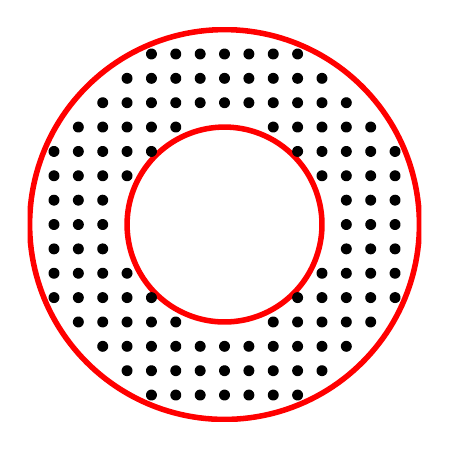
\begin{tikzpicture}

\begin{axis}[%
hide axis,
width=5cm,
height=5cm,
at={(0cm,0cm)},
scale only axis,
xmin=-10.1,
xmax=10.1,
ymin=-10.1,
ymax=10.1,
axis background/.style={fill=white}
]
\addplot [color=red, line width=2.0pt, forget plot]
  table[row sep=crcr]{%
10	0\\
9.99464587476366	-0.327190828217761\\
9.97858923238604	-0.654031292301431\\
9.95184726672197	-0.980171403295606\\
9.9144486137381	-1.30526192220052\\
9.86643332084879	-1.62895473394589\\
9.8078528040323	-1.95090322016128\\
9.73876979277334	-2.27076263034373\\
9.65925826289068	-2.58819045102521\\
9.56940335732209	-2.90284677254462\\
9.46930129495106	-3.21439465303162\\
9.35905926757326	-3.52250047921233\\
9.23879532511287	-3.8268343236509\\
9.10863824921176	-4.12707029804395\\
8.96872741532688	-4.42288690219001\\
8.81921264348355	-4.71396736825998\\
8.66025403784439	-5\\
8.49202181526579	-5.28067850650368\\
8.31469612302545	-5.55570233019602\\
8.12846684591615	-5.82477696867802\\
7.93353340291235	-6.08761429008721\\
7.73010453362737	-6.34393284163646\\
7.51839807478977	-6.59345815100069\\
7.29864072697836	-6.83592302022871\\
7.07106781186548	-7.07106781186547\\
6.83592302022871	-7.29864072697836\\
6.59345815100069	-7.51839807478977\\
6.34393284163646	-7.73010453362737\\
6.08761429008721	-7.93353340291235\\
5.82477696867802	-8.12846684591615\\
5.55570233019602	-8.31469612302545\\
5.28067850650368	-8.49202181526579\\
5	-8.66025403784439\\
4.71396736825998	-8.81921264348355\\
4.42288690219001	-8.96872741532688\\
4.12707029804395	-9.10863824921176\\
3.8268343236509	-9.23879532511287\\
3.52250047921234	-9.35905926757326\\
3.21439465303162	-9.46930129495106\\
2.90284677254462	-9.56940335732209\\
2.58819045102521	-9.65925826289068\\
2.27076263034373	-9.73876979277334\\
1.95090322016128	-9.8078528040323\\
1.62895473394589	-9.86643332084879\\
1.30526192220052	-9.9144486137381\\
0.980171403295605	-9.95184726672197\\
0.654031292301433	-9.97858923238604\\
0.327190828217762	-9.99464587476366\\
6.12323399573677e-16	-10\\
-0.32719082821776	-9.99464587476366\\
-0.654031292301431	-9.97858923238604\\
-0.980171403295604	-9.95184726672197\\
-1.30526192220052	-9.9144486137381\\
-1.62895473394589	-9.86643332084879\\
-1.95090322016128	-9.8078528040323\\
-2.27076263034373	-9.73876979277334\\
-2.58819045102521	-9.65925826289068\\
-2.90284677254462	-9.56940335732209\\
-3.21439465303162	-9.46930129495106\\
-3.52250047921233	-9.35905926757326\\
-3.8268343236509	-9.23879532511287\\
-4.12707029804395	-9.10863824921176\\
-4.42288690219001	-8.96872741532688\\
-4.71396736825998	-8.81921264348355\\
-5	-8.66025403784439\\
-5.28067850650368	-8.49202181526579\\
-5.55570233019602	-8.31469612302545\\
-5.82477696867802	-8.12846684591615\\
-6.08761429008721	-7.93353340291235\\
-6.34393284163645	-7.73010453362737\\
-6.59345815100069	-7.51839807478977\\
-6.83592302022871	-7.29864072697835\\
-7.07106781186547	-7.07106781186548\\
-7.29864072697835	-6.83592302022872\\
-7.51839807478977	-6.59345815100069\\
-7.73010453362737	-6.34393284163646\\
-7.93353340291235	-6.08761429008721\\
-8.12846684591615	-5.82477696867802\\
-8.31469612302545	-5.55570233019603\\
-8.49202181526579	-5.28067850650368\\
-8.66025403784439	-5\\
-8.81921264348355	-4.71396736825998\\
-8.96872741532688	-4.42288690219002\\
-9.10863824921176	-4.12707029804395\\
-9.23879532511287	-3.8268343236509\\
-9.35905926757326	-3.52250047921233\\
-9.46930129495106	-3.21439465303162\\
-9.56940335732209	-2.90284677254463\\
-9.65925826289068	-2.58819045102521\\
-9.73876979277334	-2.27076263034373\\
-9.8078528040323	-1.95090322016128\\
-9.86643332084879	-1.62895473394589\\
-9.9144486137381	-1.30526192220052\\
-9.95184726672197	-0.980171403295608\\
-9.97858923238604	-0.654031292301431\\
-9.99464587476366	-0.32719082821776\\
-10	-1.22464679914735e-15\\
-9.99464587476366	0.327190828217758\\
-9.97858923238604	0.654031292301429\\
-9.95184726672197	0.980171403295606\\
-9.9144486137381	1.30526192220052\\
-9.86643332084879	1.62895473394589\\
-9.80785280403231	1.95090322016128\\
-9.73876979277334	2.27076263034373\\
-9.65925826289068	2.58819045102521\\
-9.56940335732209	2.90284677254463\\
-9.46930129495106	3.21439465303162\\
-9.35905926757326	3.52250047921233\\
-9.23879532511287	3.8268343236509\\
-9.10863824921176	4.12707029804394\\
-8.96872741532688	4.42288690219001\\
-8.81921264348355	4.71396736825998\\
-8.66025403784439	5\\
-8.49202181526579	5.28067850650368\\
-8.31469612302545	5.55570233019602\\
-8.12846684591615	5.82477696867802\\
-7.93353340291235	6.08761429008721\\
-7.73010453362737	6.34393284163645\\
-7.51839807478977	6.59345815100069\\
-7.29864072697836	6.83592302022871\\
-7.07106781186548	7.07106781186547\\
-6.83592302022871	7.29864072697836\\
-6.59345815100069	7.51839807478977\\
-6.34393284163646	7.73010453362737\\
-6.08761429008721	7.93353340291235\\
-5.82477696867802	8.12846684591615\\
-5.55570233019602	8.31469612302545\\
-5.28067850650368	8.49202181526579\\
-5	8.66025403784439\\
-4.71396736825998	8.81921264348355\\
-4.42288690219001	8.96872741532688\\
-4.12707029804395	9.10863824921176\\
-3.8268343236509	9.23879532511287\\
-3.52250047921234	9.35905926757325\\
-3.21439465303162	9.46930129495106\\
-2.90284677254462	9.56940335732209\\
-2.58819045102521	9.65925826289068\\
-2.27076263034373	9.73876979277334\\
-1.95090322016129	9.8078528040323\\
-1.62895473394589	9.86643332084879\\
-1.30526192220052	9.9144486137381\\
-0.980171403295613	9.95184726672197\\
-0.654031292301427	9.97858923238604\\
-0.327190828217765	9.99464587476366\\
-1.83697019872103e-15	10\\
0.327190828217761	9.99464587476366\\
0.654031292301424	9.97858923238604\\
0.98017140329561	9.95184726672197\\
1.30526192220051	9.91444861373811\\
1.62895473394589	9.86643332084879\\
1.95090322016128	9.8078528040323\\
2.27076263034373	9.73876979277334\\
2.5881904510252	9.65925826289068\\
2.90284677254462	9.56940335732209\\
3.21439465303161	9.46930129495106\\
3.52250047921234	9.35905926757326\\
3.82683432365089	9.23879532511287\\
4.12707029804394	9.10863824921176\\
4.42288690219001	8.96872741532689\\
4.71396736825998	8.81921264348355\\
5	8.66025403784439\\
5.28067850650367	8.49202181526579\\
5.55570233019602	8.31469612302545\\
5.82477696867802	8.12846684591615\\
6.0876142900872	7.93353340291236\\
6.34393284163645	7.73010453362737\\
6.59345815100069	7.51839807478977\\
6.83592302022872	7.29864072697835\\
7.07106781186547	7.07106781186548\\
7.29864072697836	6.83592302022871\\
7.51839807478977	6.59345815100069\\
7.73010453362737	6.34393284163646\\
7.93353340291235	6.08761429008721\\
8.12846684591615	5.82477696867802\\
8.31469612302545	5.55570233019603\\
8.49202181526578	5.28067850650369\\
8.66025403784438	5\\
8.81921264348355	4.71396736825997\\
8.96872741532688	4.42288690219001\\
9.10863824921176	4.12707029804395\\
9.23879532511287	3.8268343236509\\
9.35905926757325	3.52250047921234\\
9.46930129495106	3.21439465303162\\
9.56940335732209	2.90284677254462\\
9.65925826289068	2.58819045102522\\
9.73876979277333	2.27076263034374\\
9.8078528040323	1.95090322016129\\
9.86643332084879	1.62895473394588\\
9.9144486137381	1.30526192220052\\
9.95184726672197	0.980171403295605\\
9.97858923238604	0.654031292301428\\
9.99464587476366	0.327190828217766\\
10	0\\
};
\addplot [color=red, line width=2.0pt, forget plot]
  table[row sep=crcr]{%
5	0\\
4.99732293738183	0.163595414108881\\
4.98929461619302	0.327015646150715\\
4.97592363336098	0.490085701647803\\
4.95722430686905	0.652630961100258\\
4.93321666042439	0.814477366972944\\
4.90392640201615	0.975451610080641\\
4.86938489638667	1.13538131517187\\
4.82962913144534	1.2940952255126\\
4.78470167866104	1.45142338627231\\
4.73465064747553	1.60719732651581\\
4.67952963378663	1.76125023960617\\
4.61939766255643	1.91341716182545\\
4.55431912460588	2.06353514902197\\
4.48436370766344	2.21144345109501\\
4.40960632174178	2.35698368412999\\
4.33012701892219	2.5\\
4.24601090763289	2.64033925325184\\
4.15734806151273	2.77785116509801\\
4.06423342295808	2.91238848433901\\
3.96676670145618	3.0438071450436\\
3.86505226681368	3.17196642081823\\
3.75919903739489	3.29672907550034\\
3.64932036348918	3.41796151011436\\
3.53553390593274	3.53553390593274\\
3.41796151011436	3.64932036348918\\
3.29672907550034	3.75919903739489\\
3.17196642081823	3.86505226681368\\
3.0438071450436	3.96676670145618\\
2.91238848433901	4.06423342295808\\
2.77785116509801	4.15734806151273\\
2.64033925325184	4.24601090763289\\
2.5	4.33012701892219\\
2.35698368412999	4.40960632174178\\
2.21144345109501	4.48436370766344\\
2.06353514902197	4.55431912460588\\
1.91341716182545	4.61939766255643\\
1.76125023960617	4.67952963378663\\
1.60719732651581	4.73465064747553\\
1.45142338627231	4.78470167866104\\
1.2940952255126	4.82962913144534\\
1.13538131517187	4.86938489638667\\
0.975451610080642	4.90392640201615\\
0.814477366972944	4.93321666042439\\
0.652630961100259	4.95722430686905\\
0.490085701647803	4.97592363336098\\
0.327015646150716	4.98929461619302\\
0.163595414108881	4.99732293738183\\
3.06161699786838e-16	5\\
-0.16359541410888	4.99732293738183\\
-0.327015646150716	4.98929461619302\\
-0.490085701647802	4.97592363336098\\
-0.652630961100258	4.95722430686905\\
-0.814477366972943	4.93321666042439\\
-0.975451610080641	4.90392640201615\\
-1.13538131517187	4.86938489638667\\
-1.2940952255126	4.82962913144534\\
-1.45142338627231	4.78470167866104\\
-1.60719732651581	4.73465064747553\\
-1.76125023960617	4.67952963378663\\
-1.91341716182545	4.61939766255643\\
-2.06353514902197	4.55431912460588\\
-2.21144345109501	4.48436370766344\\
-2.35698368412999	4.40960632174178\\
-2.5	4.33012701892219\\
-2.64033925325184	4.24601090763289\\
-2.77785116509801	4.15734806151273\\
-2.91238848433901	4.06423342295808\\
-3.0438071450436	3.96676670145618\\
-3.17196642081823	3.86505226681369\\
-3.29672907550034	3.75919903739489\\
-3.41796151011436	3.64932036348918\\
-3.53553390593274	3.53553390593274\\
-3.64932036348918	3.41796151011436\\
-3.75919903739489	3.29672907550034\\
-3.86505226681368	3.17196642081823\\
-3.96676670145618	3.0438071450436\\
-4.06423342295808	2.91238848433901\\
-4.15734806151273	2.77785116509801\\
-4.24601090763289	2.64033925325184\\
-4.33012701892219	2.5\\
-4.40960632174177	2.35698368412999\\
-4.48436370766344	2.21144345109501\\
-4.55431912460588	2.06353514902197\\
-4.61939766255643	1.91341716182545\\
-4.67952963378663	1.76125023960617\\
-4.73465064747553	1.60719732651581\\
-4.78470167866104	1.45142338627231\\
-4.82962913144534	1.29409522551261\\
-4.86938489638667	1.13538131517187\\
-4.90392640201615	0.975451610080641\\
-4.93321666042439	0.814477366972944\\
-4.95722430686905	0.65263096110026\\
-4.97592363336098	0.490085701647804\\
-4.98929461619302	0.327015646150716\\
-4.99732293738183	0.16359541410888\\
-5	6.12323399573677e-16\\
-4.99732293738183	-0.163595414108879\\
-4.98929461619302	-0.327015646150714\\
-4.97592363336098	-0.490085701647803\\
-4.95722430686905	-0.652630961100259\\
-4.93321666042439	-0.814477366972943\\
-4.90392640201615	-0.97545161008064\\
-4.86938489638667	-1.13538131517187\\
-4.82962913144534	-1.2940952255126\\
-4.78470167866104	-1.45142338627231\\
-4.73465064747553	-1.60719732651581\\
-4.67952963378663	-1.76125023960617\\
-4.61939766255643	-1.91341716182545\\
-4.55431912460588	-2.06353514902197\\
-4.48436370766344	-2.21144345109501\\
-4.40960632174178	-2.35698368412999\\
-4.33012701892219	-2.5\\
-4.2460109076329	-2.64033925325184\\
-4.15734806151273	-2.77785116509801\\
-4.06423342295808	-2.91238848433901\\
-3.96676670145618	-3.0438071450436\\
-3.86505226681369	-3.17196642081823\\
-3.75919903739489	-3.29672907550034\\
-3.64932036348918	-3.41796151011436\\
-3.53553390593274	-3.53553390593274\\
-3.41796151011436	-3.64932036348918\\
-3.29672907550035	-3.75919903739489\\
-3.17196642081823	-3.86505226681368\\
-3.0438071450436	-3.96676670145617\\
-2.91238848433901	-4.06423342295808\\
-2.77785116509801	-4.15734806151273\\
-2.64033925325184	-4.2460109076329\\
-2.5	-4.33012701892219\\
-2.35698368412999	-4.40960632174177\\
-2.21144345109501	-4.48436370766344\\
-2.06353514902197	-4.55431912460588\\
-1.91341716182545	-4.61939766255643\\
-1.76125023960617	-4.67952963378663\\
-1.60719732651581	-4.73465064747553\\
-1.45142338627231	-4.78470167866104\\
-1.2940952255126	-4.82962913144534\\
-1.13538131517186	-4.86938489638667\\
-0.975451610080643	-4.90392640201615\\
-0.814477366972945	-4.93321666042439\\
-0.652630961100258	-4.95722430686905\\
-0.490085701647807	-4.97592363336098\\
-0.327015646150714	-4.98929461619302\\
-0.163595414108883	-4.99732293738183\\
-9.18485099360515e-16	-5\\
0.163595414108881	-4.99732293738183\\
0.327015646150712	-4.98929461619302\\
0.490085701647805	-4.97592363336098\\
0.652630961100256	-4.95722430686905\\
0.814477366972943	-4.93321666042439\\
0.975451610080642	-4.90392640201615\\
1.13538131517186	-4.86938489638667\\
1.2940952255126	-4.82962913144534\\
1.45142338627231	-4.78470167866104\\
1.60719732651581	-4.73465064747553\\
1.76125023960617	-4.67952963378663\\
1.91341716182545	-4.61939766255643\\
2.06353514902197	-4.55431912460588\\
2.211443451095	-4.48436370766344\\
2.35698368412999	-4.40960632174178\\
2.5	-4.33012701892219\\
2.64033925325184	-4.2460109076329\\
2.77785116509801	-4.15734806151273\\
2.91238848433901	-4.06423342295808\\
3.0438071450436	-3.96676670145618\\
3.17196642081822	-3.86505226681369\\
3.29672907550035	-3.75919903739489\\
3.41796151011436	-3.64932036348918\\
3.53553390593274	-3.53553390593274\\
3.64932036348918	-3.41796151011436\\
3.75919903739489	-3.29672907550034\\
3.86505226681368	-3.17196642081823\\
3.96676670145617	-3.0438071450436\\
4.06423342295808	-2.91238848433901\\
4.15734806151272	-2.77785116509801\\
4.24601090763289	-2.64033925325184\\
4.33012701892219	-2.5\\
4.40960632174178	-2.35698368412999\\
4.48436370766344	-2.21144345109501\\
4.55431912460588	-2.06353514902197\\
4.61939766255643	-1.91341716182545\\
4.67952963378663	-1.76125023960617\\
4.73465064747553	-1.60719732651581\\
4.78470167866104	-1.45142338627231\\
4.82962913144534	-1.29409522551261\\
4.86938489638667	-1.13538131517187\\
4.90392640201615	-0.975451610080644\\
4.9332166604244	-0.814477366972941\\
4.95722430686905	-0.652630961100258\\
4.97592363336098	-0.490085701647803\\
4.98929461619302	-0.327015646150714\\
4.99732293738183	-0.163595414108883\\
5	0\\
};

\addplot[area legend, draw=black, fill=black, forget plot]
table[row sep=crcr] {%
x	y\\
-3.5	-8.75\\
-3.50480367989919	-8.70122741949597\\
-3.51903011687218	-8.65432914190873\\
-3.54213259692436	-8.6111074417451\\
-3.57322330470336	-8.57322330470336\\
-3.6111074417451	-8.54213259692436\\
-3.65432914190873	-8.51903011687218\\
-3.70122741949597	-8.50480367989919\\
-3.75	-8.5\\
-3.79877258050403	-8.50480367989919\\
-3.84567085809127	-8.51903011687218\\
-3.8888925582549	-8.54213259692436\\
-3.92677669529664	-8.57322330470336\\
-3.95786740307564	-8.6111074417451\\
-3.98096988312782	-8.65432914190873\\
-3.99519632010081	-8.70122741949597\\
-4	-8.75\\
-3.99519632010081	-8.79877258050403\\
-3.98096988312782	-8.84567085809127\\
-3.95786740307564	-8.8888925582549\\
-3.92677669529664	-8.92677669529664\\
-3.8888925582549	-8.95786740307564\\
-3.84567085809127	-8.98096988312782\\
-3.79877258050403	-8.99519632010081\\
-3.75	-9\\
-3.70122741949597	-8.99519632010081\\
-3.65432914190873	-8.98096988312782\\
-3.6111074417451	-8.95786740307564\\
-3.57322330470336	-8.92677669529664\\
-3.54213259692436	-8.8888925582549\\
-3.51903011687218	-8.84567085809127\\
-3.50480367989919	-8.79877258050403\\
-3.5	-8.75\\
}--cycle;

\addplot[area legend, draw=black, fill=black, forget plot]
table[row sep=crcr] {%
x	y\\
-2.25	-8.75\\
-2.25480367989919	-8.70122741949597\\
-2.26903011687218	-8.65432914190873\\
-2.29213259692436	-8.6111074417451\\
-2.32322330470336	-8.57322330470336\\
-2.3611074417451	-8.54213259692436\\
-2.40432914190873	-8.51903011687218\\
-2.45122741949597	-8.50480367989919\\
-2.5	-8.5\\
-2.54877258050403	-8.50480367989919\\
-2.59567085809127	-8.51903011687218\\
-2.6388925582549	-8.54213259692436\\
-2.67677669529664	-8.57322330470336\\
-2.70786740307564	-8.6111074417451\\
-2.73096988312782	-8.65432914190873\\
-2.74519632010081	-8.70122741949597\\
-2.75	-8.75\\
-2.74519632010081	-8.79877258050403\\
-2.73096988312782	-8.84567085809127\\
-2.70786740307564	-8.8888925582549\\
-2.67677669529664	-8.92677669529664\\
-2.6388925582549	-8.95786740307564\\
-2.59567085809127	-8.98096988312782\\
-2.54877258050403	-8.99519632010081\\
-2.5	-9\\
-2.45122741949597	-8.99519632010081\\
-2.40432914190873	-8.98096988312782\\
-2.3611074417451	-8.95786740307564\\
-2.32322330470336	-8.92677669529664\\
-2.29213259692436	-8.8888925582549\\
-2.26903011687218	-8.84567085809127\\
-2.25480367989919	-8.79877258050403\\
-2.25	-8.75\\
}--cycle;

\addplot[area legend, draw=black, fill=black, forget plot]
table[row sep=crcr] {%
x	y\\
-1	-8.75\\
-1.00480367989919	-8.70122741949597\\
-1.01903011687218	-8.65432914190873\\
-1.04213259692436	-8.6111074417451\\
-1.07322330470336	-8.57322330470336\\
-1.1111074417451	-8.54213259692436\\
-1.15432914190873	-8.51903011687218\\
-1.20122741949597	-8.50480367989919\\
-1.25	-8.5\\
-1.29877258050403	-8.50480367989919\\
-1.34567085809127	-8.51903011687218\\
-1.3888925582549	-8.54213259692436\\
-1.42677669529664	-8.57322330470336\\
-1.45786740307564	-8.6111074417451\\
-1.48096988312782	-8.65432914190873\\
-1.49519632010081	-8.70122741949597\\
-1.5	-8.75\\
-1.49519632010081	-8.79877258050403\\
-1.48096988312782	-8.84567085809127\\
-1.45786740307564	-8.8888925582549\\
-1.42677669529664	-8.92677669529664\\
-1.3888925582549	-8.95786740307564\\
-1.34567085809127	-8.98096988312782\\
-1.29877258050403	-8.99519632010081\\
-1.25	-9\\
-1.20122741949597	-8.99519632010081\\
-1.15432914190873	-8.98096988312782\\
-1.1111074417451	-8.95786740307564\\
-1.07322330470336	-8.92677669529664\\
-1.04213259692436	-8.8888925582549\\
-1.01903011687218	-8.84567085809127\\
-1.00480367989919	-8.79877258050403\\
-1	-8.75\\
}--cycle;

\addplot[area legend, draw=black, fill=black, forget plot]
table[row sep=crcr] {%
x	y\\
0.25	-8.75\\
0.245196320100808	-8.70122741949597\\
0.230969883127822	-8.65432914190873\\
0.207867403075636	-8.6111074417451\\
0.176776695296637	-8.57322330470336\\
0.138892558254901	-8.54213259692436\\
0.0956708580912725	-8.51903011687218\\
0.0487725805040321	-8.50480367989919\\
1.53080849893419e-17	-8.5\\
-0.048772580504032	-8.50480367989919\\
-0.0956708580912724	-8.51903011687218\\
-0.138892558254901	-8.54213259692436\\
-0.176776695296637	-8.57322330470336\\
-0.207867403075636	-8.6111074417451\\
-0.230969883127822	-8.65432914190873\\
-0.245196320100808	-8.70122741949597\\
-0.25	-8.75\\
-0.245196320100808	-8.79877258050403\\
-0.230969883127822	-8.84567085809127\\
-0.207867403075636	-8.8888925582549\\
-0.176776695296637	-8.92677669529664\\
-0.138892558254901	-8.95786740307564\\
-0.0956708580912726	-8.98096988312782\\
-0.0487725805040322	-8.99519632010081\\
-4.59242549680257e-17	-9\\
0.0487725805040321	-8.99519632010081\\
0.0956708580912725	-8.98096988312782\\
0.1388925582549	-8.95786740307564\\
0.176776695296637	-8.92677669529664\\
0.207867403075636	-8.8888925582549\\
0.230969883127822	-8.84567085809127\\
0.245196320100808	-8.79877258050403\\
0.25	-8.75\\
}--cycle;

\addplot[area legend, draw=black, fill=black, forget plot]
table[row sep=crcr] {%
x	y\\
1.5	-8.75\\
1.49519632010081	-8.70122741949597\\
1.48096988312782	-8.65432914190873\\
1.45786740307564	-8.6111074417451\\
1.42677669529664	-8.57322330470336\\
1.3888925582549	-8.54213259692436\\
1.34567085809127	-8.51903011687218\\
1.29877258050403	-8.50480367989919\\
1.25	-8.5\\
1.20122741949597	-8.50480367989919\\
1.15432914190873	-8.51903011687218\\
1.1111074417451	-8.54213259692436\\
1.07322330470336	-8.57322330470336\\
1.04213259692436	-8.6111074417451\\
1.01903011687218	-8.65432914190873\\
1.00480367989919	-8.70122741949597\\
1	-8.75\\
1.00480367989919	-8.79877258050403\\
1.01903011687218	-8.84567085809127\\
1.04213259692436	-8.8888925582549\\
1.07322330470336	-8.92677669529664\\
1.1111074417451	-8.95786740307564\\
1.15432914190873	-8.98096988312782\\
1.20122741949597	-8.99519632010081\\
1.25	-9\\
1.29877258050403	-8.99519632010081\\
1.34567085809127	-8.98096988312782\\
1.3888925582549	-8.95786740307564\\
1.42677669529664	-8.92677669529664\\
1.45786740307564	-8.8888925582549\\
1.48096988312782	-8.84567085809127\\
1.49519632010081	-8.79877258050403\\
1.5	-8.75\\
}--cycle;

\addplot[area legend, draw=black, fill=black, forget plot]
table[row sep=crcr] {%
x	y\\
2.75	-8.75\\
2.74519632010081	-8.70122741949597\\
2.73096988312782	-8.65432914190873\\
2.70786740307564	-8.6111074417451\\
2.67677669529664	-8.57322330470336\\
2.6388925582549	-8.54213259692436\\
2.59567085809127	-8.51903011687218\\
2.54877258050403	-8.50480367989919\\
2.5	-8.5\\
2.45122741949597	-8.50480367989919\\
2.40432914190873	-8.51903011687218\\
2.3611074417451	-8.54213259692436\\
2.32322330470336	-8.57322330470336\\
2.29213259692436	-8.6111074417451\\
2.26903011687218	-8.65432914190873\\
2.25480367989919	-8.70122741949597\\
2.25	-8.75\\
2.25480367989919	-8.79877258050403\\
2.26903011687218	-8.84567085809127\\
2.29213259692436	-8.8888925582549\\
2.32322330470336	-8.92677669529664\\
2.3611074417451	-8.95786740307564\\
2.40432914190873	-8.98096988312782\\
2.45122741949597	-8.99519632010081\\
2.5	-9\\
2.54877258050403	-8.99519632010081\\
2.59567085809127	-8.98096988312782\\
2.6388925582549	-8.95786740307564\\
2.67677669529664	-8.92677669529664\\
2.70786740307564	-8.8888925582549\\
2.73096988312782	-8.84567085809127\\
2.74519632010081	-8.79877258050403\\
2.75	-8.75\\
}--cycle;

\addplot[area legend, draw=black, fill=black, forget plot]
table[row sep=crcr] {%
x	y\\
4	-8.75\\
3.99519632010081	-8.70122741949597\\
3.98096988312782	-8.65432914190873\\
3.95786740307564	-8.6111074417451\\
3.92677669529664	-8.57322330470336\\
3.8888925582549	-8.54213259692436\\
3.84567085809127	-8.51903011687218\\
3.79877258050403	-8.50480367989919\\
3.75	-8.5\\
3.70122741949597	-8.50480367989919\\
3.65432914190873	-8.51903011687218\\
3.6111074417451	-8.54213259692436\\
3.57322330470336	-8.57322330470336\\
3.54213259692436	-8.6111074417451\\
3.51903011687218	-8.65432914190873\\
3.50480367989919	-8.70122741949597\\
3.5	-8.75\\
3.50480367989919	-8.79877258050403\\
3.51903011687218	-8.84567085809127\\
3.54213259692436	-8.8888925582549\\
3.57322330470336	-8.92677669529664\\
3.6111074417451	-8.95786740307564\\
3.65432914190873	-8.98096988312782\\
3.70122741949597	-8.99519632010081\\
3.75	-9\\
3.79877258050403	-8.99519632010081\\
3.84567085809127	-8.98096988312782\\
3.8888925582549	-8.95786740307564\\
3.92677669529664	-8.92677669529664\\
3.95786740307564	-8.8888925582549\\
3.98096988312782	-8.84567085809127\\
3.99519632010081	-8.79877258050403\\
4	-8.75\\
}--cycle;

\addplot[area legend, draw=black, fill=black, forget plot]
table[row sep=crcr] {%
x	y\\
-4.75	-7.5\\
-4.75480367989919	-7.45122741949597\\
-4.76903011687218	-7.40432914190873\\
-4.79213259692436	-7.3611074417451\\
-4.82322330470336	-7.32322330470336\\
-4.8611074417451	-7.29213259692436\\
-4.90432914190873	-7.26903011687218\\
-4.95122741949597	-7.25480367989919\\
-5	-7.25\\
-5.04877258050403	-7.25480367989919\\
-5.09567085809127	-7.26903011687218\\
-5.1388925582549	-7.29213259692436\\
-5.17677669529664	-7.32322330470336\\
-5.20786740307564	-7.3611074417451\\
-5.23096988312782	-7.40432914190873\\
-5.24519632010081	-7.45122741949597\\
-5.25	-7.5\\
-5.24519632010081	-7.54877258050403\\
-5.23096988312782	-7.59567085809127\\
-5.20786740307564	-7.6388925582549\\
-5.17677669529664	-7.67677669529664\\
-5.1388925582549	-7.70786740307564\\
-5.09567085809127	-7.73096988312782\\
-5.04877258050403	-7.74519632010081\\
-5	-7.75\\
-4.95122741949597	-7.74519632010081\\
-4.90432914190873	-7.73096988312782\\
-4.8611074417451	-7.70786740307564\\
-4.82322330470336	-7.67677669529664\\
-4.79213259692436	-7.6388925582549\\
-4.76903011687218	-7.59567085809127\\
-4.75480367989919	-7.54877258050403\\
-4.75	-7.5\\
}--cycle;

\addplot[area legend, draw=black, fill=black, forget plot]
table[row sep=crcr] {%
x	y\\
-3.5	-7.5\\
-3.50480367989919	-7.45122741949597\\
-3.51903011687218	-7.40432914190873\\
-3.54213259692436	-7.3611074417451\\
-3.57322330470336	-7.32322330470336\\
-3.6111074417451	-7.29213259692436\\
-3.65432914190873	-7.26903011687218\\
-3.70122741949597	-7.25480367989919\\
-3.75	-7.25\\
-3.79877258050403	-7.25480367989919\\
-3.84567085809127	-7.26903011687218\\
-3.8888925582549	-7.29213259692436\\
-3.92677669529664	-7.32322330470336\\
-3.95786740307564	-7.3611074417451\\
-3.98096988312782	-7.40432914190873\\
-3.99519632010081	-7.45122741949597\\
-4	-7.5\\
-3.99519632010081	-7.54877258050403\\
-3.98096988312782	-7.59567085809127\\
-3.95786740307564	-7.6388925582549\\
-3.92677669529664	-7.67677669529664\\
-3.8888925582549	-7.70786740307564\\
-3.84567085809127	-7.73096988312782\\
-3.79877258050403	-7.74519632010081\\
-3.75	-7.75\\
-3.70122741949597	-7.74519632010081\\
-3.65432914190873	-7.73096988312782\\
-3.6111074417451	-7.70786740307564\\
-3.57322330470336	-7.67677669529664\\
-3.54213259692436	-7.6388925582549\\
-3.51903011687218	-7.59567085809127\\
-3.50480367989919	-7.54877258050403\\
-3.5	-7.5\\
}--cycle;

\addplot[area legend, draw=black, fill=black, forget plot]
table[row sep=crcr] {%
x	y\\
-2.25	-7.5\\
-2.25480367989919	-7.45122741949597\\
-2.26903011687218	-7.40432914190873\\
-2.29213259692436	-7.3611074417451\\
-2.32322330470336	-7.32322330470336\\
-2.3611074417451	-7.29213259692436\\
-2.40432914190873	-7.26903011687218\\
-2.45122741949597	-7.25480367989919\\
-2.5	-7.25\\
-2.54877258050403	-7.25480367989919\\
-2.59567085809127	-7.26903011687218\\
-2.6388925582549	-7.29213259692436\\
-2.67677669529664	-7.32322330470336\\
-2.70786740307564	-7.3611074417451\\
-2.73096988312782	-7.40432914190873\\
-2.74519632010081	-7.45122741949597\\
-2.75	-7.5\\
-2.74519632010081	-7.54877258050403\\
-2.73096988312782	-7.59567085809127\\
-2.70786740307564	-7.6388925582549\\
-2.67677669529664	-7.67677669529664\\
-2.6388925582549	-7.70786740307564\\
-2.59567085809127	-7.73096988312782\\
-2.54877258050403	-7.74519632010081\\
-2.5	-7.75\\
-2.45122741949597	-7.74519632010081\\
-2.40432914190873	-7.73096988312782\\
-2.3611074417451	-7.70786740307564\\
-2.32322330470336	-7.67677669529664\\
-2.29213259692436	-7.6388925582549\\
-2.26903011687218	-7.59567085809127\\
-2.25480367989919	-7.54877258050403\\
-2.25	-7.5\\
}--cycle;

\addplot[area legend, draw=black, fill=black, forget plot]
table[row sep=crcr] {%
x	y\\
-1	-7.5\\
-1.00480367989919	-7.45122741949597\\
-1.01903011687218	-7.40432914190873\\
-1.04213259692436	-7.3611074417451\\
-1.07322330470336	-7.32322330470336\\
-1.1111074417451	-7.29213259692436\\
-1.15432914190873	-7.26903011687218\\
-1.20122741949597	-7.25480367989919\\
-1.25	-7.25\\
-1.29877258050403	-7.25480367989919\\
-1.34567085809127	-7.26903011687218\\
-1.3888925582549	-7.29213259692436\\
-1.42677669529664	-7.32322330470336\\
-1.45786740307564	-7.3611074417451\\
-1.48096988312782	-7.40432914190873\\
-1.49519632010081	-7.45122741949597\\
-1.5	-7.5\\
-1.49519632010081	-7.54877258050403\\
-1.48096988312782	-7.59567085809127\\
-1.45786740307564	-7.6388925582549\\
-1.42677669529664	-7.67677669529664\\
-1.3888925582549	-7.70786740307564\\
-1.34567085809127	-7.73096988312782\\
-1.29877258050403	-7.74519632010081\\
-1.25	-7.75\\
-1.20122741949597	-7.74519632010081\\
-1.15432914190873	-7.73096988312782\\
-1.1111074417451	-7.70786740307564\\
-1.07322330470336	-7.67677669529664\\
-1.04213259692436	-7.6388925582549\\
-1.01903011687218	-7.59567085809127\\
-1.00480367989919	-7.54877258050403\\
-1	-7.5\\
}--cycle;

\addplot[area legend, draw=black, fill=black, forget plot]
table[row sep=crcr] {%
x	y\\
0.25	-7.5\\
0.245196320100808	-7.45122741949597\\
0.230969883127822	-7.40432914190873\\
0.207867403075636	-7.3611074417451\\
0.176776695296637	-7.32322330470336\\
0.138892558254901	-7.29213259692436\\
0.0956708580912725	-7.26903011687218\\
0.0487725805040321	-7.25480367989919\\
1.53080849893419e-17	-7.25\\
-0.048772580504032	-7.25480367989919\\
-0.0956708580912724	-7.26903011687218\\
-0.138892558254901	-7.29213259692436\\
-0.176776695296637	-7.32322330470336\\
-0.207867403075636	-7.3611074417451\\
-0.230969883127822	-7.40432914190873\\
-0.245196320100808	-7.45122741949597\\
-0.25	-7.5\\
-0.245196320100808	-7.54877258050403\\
-0.230969883127822	-7.59567085809127\\
-0.207867403075636	-7.6388925582549\\
-0.176776695296637	-7.67677669529664\\
-0.138892558254901	-7.70786740307564\\
-0.0956708580912726	-7.73096988312782\\
-0.0487725805040322	-7.74519632010081\\
-4.59242549680257e-17	-7.75\\
0.0487725805040321	-7.74519632010081\\
0.0956708580912725	-7.73096988312782\\
0.1388925582549	-7.70786740307564\\
0.176776695296637	-7.67677669529664\\
0.207867403075636	-7.6388925582549\\
0.230969883127822	-7.59567085809127\\
0.245196320100808	-7.54877258050403\\
0.25	-7.5\\
}--cycle;

\addplot[area legend, draw=black, fill=black, forget plot]
table[row sep=crcr] {%
x	y\\
1.5	-7.5\\
1.49519632010081	-7.45122741949597\\
1.48096988312782	-7.40432914190873\\
1.45786740307564	-7.3611074417451\\
1.42677669529664	-7.32322330470336\\
1.3888925582549	-7.29213259692436\\
1.34567085809127	-7.26903011687218\\
1.29877258050403	-7.25480367989919\\
1.25	-7.25\\
1.20122741949597	-7.25480367989919\\
1.15432914190873	-7.26903011687218\\
1.1111074417451	-7.29213259692436\\
1.07322330470336	-7.32322330470336\\
1.04213259692436	-7.3611074417451\\
1.01903011687218	-7.40432914190873\\
1.00480367989919	-7.45122741949597\\
1	-7.5\\
1.00480367989919	-7.54877258050403\\
1.01903011687218	-7.59567085809127\\
1.04213259692436	-7.6388925582549\\
1.07322330470336	-7.67677669529664\\
1.1111074417451	-7.70786740307564\\
1.15432914190873	-7.73096988312782\\
1.20122741949597	-7.74519632010081\\
1.25	-7.75\\
1.29877258050403	-7.74519632010081\\
1.34567085809127	-7.73096988312782\\
1.3888925582549	-7.70786740307564\\
1.42677669529664	-7.67677669529664\\
1.45786740307564	-7.6388925582549\\
1.48096988312782	-7.59567085809127\\
1.49519632010081	-7.54877258050403\\
1.5	-7.5\\
}--cycle;

\addplot[area legend, draw=black, fill=black, forget plot]
table[row sep=crcr] {%
x	y\\
2.75	-7.5\\
2.74519632010081	-7.45122741949597\\
2.73096988312782	-7.40432914190873\\
2.70786740307564	-7.3611074417451\\
2.67677669529664	-7.32322330470336\\
2.6388925582549	-7.29213259692436\\
2.59567085809127	-7.26903011687218\\
2.54877258050403	-7.25480367989919\\
2.5	-7.25\\
2.45122741949597	-7.25480367989919\\
2.40432914190873	-7.26903011687218\\
2.3611074417451	-7.29213259692436\\
2.32322330470336	-7.32322330470336\\
2.29213259692436	-7.3611074417451\\
2.26903011687218	-7.40432914190873\\
2.25480367989919	-7.45122741949597\\
2.25	-7.5\\
2.25480367989919	-7.54877258050403\\
2.26903011687218	-7.59567085809127\\
2.29213259692436	-7.6388925582549\\
2.32322330470336	-7.67677669529664\\
2.3611074417451	-7.70786740307564\\
2.40432914190873	-7.73096988312782\\
2.45122741949597	-7.74519632010081\\
2.5	-7.75\\
2.54877258050403	-7.74519632010081\\
2.59567085809127	-7.73096988312782\\
2.6388925582549	-7.70786740307564\\
2.67677669529664	-7.67677669529664\\
2.70786740307564	-7.6388925582549\\
2.73096988312782	-7.59567085809127\\
2.74519632010081	-7.54877258050403\\
2.75	-7.5\\
}--cycle;

\addplot[area legend, draw=black, fill=black, forget plot]
table[row sep=crcr] {%
x	y\\
4	-7.5\\
3.99519632010081	-7.45122741949597\\
3.98096988312782	-7.40432914190873\\
3.95786740307564	-7.3611074417451\\
3.92677669529664	-7.32322330470336\\
3.8888925582549	-7.29213259692436\\
3.84567085809127	-7.26903011687218\\
3.79877258050403	-7.25480367989919\\
3.75	-7.25\\
3.70122741949597	-7.25480367989919\\
3.65432914190873	-7.26903011687218\\
3.6111074417451	-7.29213259692436\\
3.57322330470336	-7.32322330470336\\
3.54213259692436	-7.3611074417451\\
3.51903011687218	-7.40432914190873\\
3.50480367989919	-7.45122741949597\\
3.5	-7.5\\
3.50480367989919	-7.54877258050403\\
3.51903011687218	-7.59567085809127\\
3.54213259692436	-7.6388925582549\\
3.57322330470336	-7.67677669529664\\
3.6111074417451	-7.70786740307564\\
3.65432914190873	-7.73096988312782\\
3.70122741949597	-7.74519632010081\\
3.75	-7.75\\
3.79877258050403	-7.74519632010081\\
3.84567085809127	-7.73096988312782\\
3.8888925582549	-7.70786740307564\\
3.92677669529664	-7.67677669529664\\
3.95786740307564	-7.6388925582549\\
3.98096988312782	-7.59567085809127\\
3.99519632010081	-7.54877258050403\\
4	-7.5\\
}--cycle;

\addplot[area legend, draw=black, fill=black, forget plot]
table[row sep=crcr] {%
x	y\\
5.25	-7.5\\
5.24519632010081	-7.45122741949597\\
5.23096988312782	-7.40432914190873\\
5.20786740307564	-7.3611074417451\\
5.17677669529664	-7.32322330470336\\
5.1388925582549	-7.29213259692436\\
5.09567085809127	-7.26903011687218\\
5.04877258050403	-7.25480367989919\\
5	-7.25\\
4.95122741949597	-7.25480367989919\\
4.90432914190873	-7.26903011687218\\
4.8611074417451	-7.29213259692436\\
4.82322330470336	-7.32322330470336\\
4.79213259692436	-7.3611074417451\\
4.76903011687218	-7.40432914190873\\
4.75480367989919	-7.45122741949597\\
4.75	-7.5\\
4.75480367989919	-7.54877258050403\\
4.76903011687218	-7.59567085809127\\
4.79213259692436	-7.6388925582549\\
4.82322330470336	-7.67677669529664\\
4.8611074417451	-7.70786740307564\\
4.90432914190873	-7.73096988312782\\
4.95122741949597	-7.74519632010081\\
5	-7.75\\
5.04877258050403	-7.74519632010081\\
5.09567085809127	-7.73096988312782\\
5.1388925582549	-7.70786740307564\\
5.17677669529664	-7.67677669529664\\
5.20786740307564	-7.6388925582549\\
5.23096988312782	-7.59567085809127\\
5.24519632010081	-7.54877258050403\\
5.25	-7.5\\
}--cycle;

\addplot[area legend, draw=black, fill=black, forget plot]
table[row sep=crcr] {%
x	y\\
-6	-6.25\\
-6.00480367989919	-6.20122741949597\\
-6.01903011687218	-6.15432914190873\\
-6.04213259692436	-6.1111074417451\\
-6.07322330470336	-6.07322330470336\\
-6.1111074417451	-6.04213259692436\\
-6.15432914190873	-6.01903011687218\\
-6.20122741949597	-6.00480367989919\\
-6.25	-6\\
-6.29877258050403	-6.00480367989919\\
-6.34567085809127	-6.01903011687218\\
-6.3888925582549	-6.04213259692436\\
-6.42677669529664	-6.07322330470336\\
-6.45786740307564	-6.1111074417451\\
-6.48096988312782	-6.15432914190873\\
-6.49519632010081	-6.20122741949597\\
-6.5	-6.25\\
-6.49519632010081	-6.29877258050403\\
-6.48096988312782	-6.34567085809127\\
-6.45786740307564	-6.3888925582549\\
-6.42677669529664	-6.42677669529664\\
-6.3888925582549	-6.45786740307564\\
-6.34567085809127	-6.48096988312782\\
-6.29877258050403	-6.49519632010081\\
-6.25	-6.5\\
-6.20122741949597	-6.49519632010081\\
-6.15432914190873	-6.48096988312782\\
-6.1111074417451	-6.45786740307564\\
-6.07322330470336	-6.42677669529664\\
-6.04213259692436	-6.3888925582549\\
-6.01903011687218	-6.34567085809127\\
-6.00480367989919	-6.29877258050403\\
-6	-6.25\\
}--cycle;

\addplot[area legend, draw=black, fill=black, forget plot]
table[row sep=crcr] {%
x	y\\
-4.75	-6.25\\
-4.75480367989919	-6.20122741949597\\
-4.76903011687218	-6.15432914190873\\
-4.79213259692436	-6.1111074417451\\
-4.82322330470336	-6.07322330470336\\
-4.8611074417451	-6.04213259692436\\
-4.90432914190873	-6.01903011687218\\
-4.95122741949597	-6.00480367989919\\
-5	-6\\
-5.04877258050403	-6.00480367989919\\
-5.09567085809127	-6.01903011687218\\
-5.1388925582549	-6.04213259692436\\
-5.17677669529664	-6.07322330470336\\
-5.20786740307564	-6.1111074417451\\
-5.23096988312782	-6.15432914190873\\
-5.24519632010081	-6.20122741949597\\
-5.25	-6.25\\
-5.24519632010081	-6.29877258050403\\
-5.23096988312782	-6.34567085809127\\
-5.20786740307564	-6.3888925582549\\
-5.17677669529664	-6.42677669529664\\
-5.1388925582549	-6.45786740307564\\
-5.09567085809127	-6.48096988312782\\
-5.04877258050403	-6.49519632010081\\
-5	-6.5\\
-4.95122741949597	-6.49519632010081\\
-4.90432914190873	-6.48096988312782\\
-4.8611074417451	-6.45786740307564\\
-4.82322330470336	-6.42677669529664\\
-4.79213259692436	-6.3888925582549\\
-4.76903011687218	-6.34567085809127\\
-4.75480367989919	-6.29877258050403\\
-4.75	-6.25\\
}--cycle;

\addplot[area legend, draw=black, fill=black, forget plot]
table[row sep=crcr] {%
x	y\\
-3.5	-6.25\\
-3.50480367989919	-6.20122741949597\\
-3.51903011687218	-6.15432914190873\\
-3.54213259692436	-6.1111074417451\\
-3.57322330470336	-6.07322330470336\\
-3.6111074417451	-6.04213259692436\\
-3.65432914190873	-6.01903011687218\\
-3.70122741949597	-6.00480367989919\\
-3.75	-6\\
-3.79877258050403	-6.00480367989919\\
-3.84567085809127	-6.01903011687218\\
-3.8888925582549	-6.04213259692436\\
-3.92677669529664	-6.07322330470336\\
-3.95786740307564	-6.1111074417451\\
-3.98096988312782	-6.15432914190873\\
-3.99519632010081	-6.20122741949597\\
-4	-6.25\\
-3.99519632010081	-6.29877258050403\\
-3.98096988312782	-6.34567085809127\\
-3.95786740307564	-6.3888925582549\\
-3.92677669529664	-6.42677669529664\\
-3.8888925582549	-6.45786740307564\\
-3.84567085809127	-6.48096988312782\\
-3.79877258050403	-6.49519632010081\\
-3.75	-6.5\\
-3.70122741949597	-6.49519632010081\\
-3.65432914190873	-6.48096988312782\\
-3.6111074417451	-6.45786740307564\\
-3.57322330470336	-6.42677669529664\\
-3.54213259692436	-6.3888925582549\\
-3.51903011687218	-6.34567085809127\\
-3.50480367989919	-6.29877258050403\\
-3.5	-6.25\\
}--cycle;

\addplot[area legend, draw=black, fill=black, forget plot]
table[row sep=crcr] {%
x	y\\
-2.25	-6.25\\
-2.25480367989919	-6.20122741949597\\
-2.26903011687218	-6.15432914190873\\
-2.29213259692436	-6.1111074417451\\
-2.32322330470336	-6.07322330470336\\
-2.3611074417451	-6.04213259692436\\
-2.40432914190873	-6.01903011687218\\
-2.45122741949597	-6.00480367989919\\
-2.5	-6\\
-2.54877258050403	-6.00480367989919\\
-2.59567085809127	-6.01903011687218\\
-2.6388925582549	-6.04213259692436\\
-2.67677669529664	-6.07322330470336\\
-2.70786740307564	-6.1111074417451\\
-2.73096988312782	-6.15432914190873\\
-2.74519632010081	-6.20122741949597\\
-2.75	-6.25\\
-2.74519632010081	-6.29877258050403\\
-2.73096988312782	-6.34567085809127\\
-2.70786740307564	-6.3888925582549\\
-2.67677669529664	-6.42677669529664\\
-2.6388925582549	-6.45786740307564\\
-2.59567085809127	-6.48096988312782\\
-2.54877258050403	-6.49519632010081\\
-2.5	-6.5\\
-2.45122741949597	-6.49519632010081\\
-2.40432914190873	-6.48096988312782\\
-2.3611074417451	-6.45786740307564\\
-2.32322330470336	-6.42677669529664\\
-2.29213259692436	-6.3888925582549\\
-2.26903011687218	-6.34567085809127\\
-2.25480367989919	-6.29877258050403\\
-2.25	-6.25\\
}--cycle;

\addplot[area legend, draw=black, fill=black, forget plot]
table[row sep=crcr] {%
x	y\\
-1	-6.25\\
-1.00480367989919	-6.20122741949597\\
-1.01903011687218	-6.15432914190873\\
-1.04213259692436	-6.1111074417451\\
-1.07322330470336	-6.07322330470336\\
-1.1111074417451	-6.04213259692436\\
-1.15432914190873	-6.01903011687218\\
-1.20122741949597	-6.00480367989919\\
-1.25	-6\\
-1.29877258050403	-6.00480367989919\\
-1.34567085809127	-6.01903011687218\\
-1.3888925582549	-6.04213259692436\\
-1.42677669529664	-6.07322330470336\\
-1.45786740307564	-6.1111074417451\\
-1.48096988312782	-6.15432914190873\\
-1.49519632010081	-6.20122741949597\\
-1.5	-6.25\\
-1.49519632010081	-6.29877258050403\\
-1.48096988312782	-6.34567085809127\\
-1.45786740307564	-6.3888925582549\\
-1.42677669529664	-6.42677669529664\\
-1.3888925582549	-6.45786740307564\\
-1.34567085809127	-6.48096988312782\\
-1.29877258050403	-6.49519632010081\\
-1.25	-6.5\\
-1.20122741949597	-6.49519632010081\\
-1.15432914190873	-6.48096988312782\\
-1.1111074417451	-6.45786740307564\\
-1.07322330470336	-6.42677669529664\\
-1.04213259692436	-6.3888925582549\\
-1.01903011687218	-6.34567085809127\\
-1.00480367989919	-6.29877258050403\\
-1	-6.25\\
}--cycle;

\addplot[area legend, draw=black, fill=black, forget plot]
table[row sep=crcr] {%
x	y\\
0.25	-6.25\\
0.245196320100808	-6.20122741949597\\
0.230969883127822	-6.15432914190873\\
0.207867403075636	-6.1111074417451\\
0.176776695296637	-6.07322330470336\\
0.138892558254901	-6.04213259692436\\
0.0956708580912725	-6.01903011687218\\
0.0487725805040321	-6.00480367989919\\
1.53080849893419e-17	-6\\
-0.048772580504032	-6.00480367989919\\
-0.0956708580912724	-6.01903011687218\\
-0.138892558254901	-6.04213259692436\\
-0.176776695296637	-6.07322330470336\\
-0.207867403075636	-6.1111074417451\\
-0.230969883127822	-6.15432914190873\\
-0.245196320100808	-6.20122741949597\\
-0.25	-6.25\\
-0.245196320100808	-6.29877258050403\\
-0.230969883127822	-6.34567085809127\\
-0.207867403075636	-6.3888925582549\\
-0.176776695296637	-6.42677669529664\\
-0.138892558254901	-6.45786740307564\\
-0.0956708580912726	-6.48096988312782\\
-0.0487725805040322	-6.49519632010081\\
-4.59242549680257e-17	-6.5\\
0.0487725805040321	-6.49519632010081\\
0.0956708580912725	-6.48096988312782\\
0.1388925582549	-6.45786740307564\\
0.176776695296637	-6.42677669529664\\
0.207867403075636	-6.3888925582549\\
0.230969883127822	-6.34567085809127\\
0.245196320100808	-6.29877258050403\\
0.25	-6.25\\
}--cycle;

\addplot[area legend, draw=black, fill=black, forget plot]
table[row sep=crcr] {%
x	y\\
1.5	-6.25\\
1.49519632010081	-6.20122741949597\\
1.48096988312782	-6.15432914190873\\
1.45786740307564	-6.1111074417451\\
1.42677669529664	-6.07322330470336\\
1.3888925582549	-6.04213259692436\\
1.34567085809127	-6.01903011687218\\
1.29877258050403	-6.00480367989919\\
1.25	-6\\
1.20122741949597	-6.00480367989919\\
1.15432914190873	-6.01903011687218\\
1.1111074417451	-6.04213259692436\\
1.07322330470336	-6.07322330470336\\
1.04213259692436	-6.1111074417451\\
1.01903011687218	-6.15432914190873\\
1.00480367989919	-6.20122741949597\\
1	-6.25\\
1.00480367989919	-6.29877258050403\\
1.01903011687218	-6.34567085809127\\
1.04213259692436	-6.3888925582549\\
1.07322330470336	-6.42677669529664\\
1.1111074417451	-6.45786740307564\\
1.15432914190873	-6.48096988312782\\
1.20122741949597	-6.49519632010081\\
1.25	-6.5\\
1.29877258050403	-6.49519632010081\\
1.34567085809127	-6.48096988312782\\
1.3888925582549	-6.45786740307564\\
1.42677669529664	-6.42677669529664\\
1.45786740307564	-6.3888925582549\\
1.48096988312782	-6.34567085809127\\
1.49519632010081	-6.29877258050403\\
1.5	-6.25\\
}--cycle;

\addplot[area legend, draw=black, fill=black, forget plot]
table[row sep=crcr] {%
x	y\\
2.75	-6.25\\
2.74519632010081	-6.20122741949597\\
2.73096988312782	-6.15432914190873\\
2.70786740307564	-6.1111074417451\\
2.67677669529664	-6.07322330470336\\
2.6388925582549	-6.04213259692436\\
2.59567085809127	-6.01903011687218\\
2.54877258050403	-6.00480367989919\\
2.5	-6\\
2.45122741949597	-6.00480367989919\\
2.40432914190873	-6.01903011687218\\
2.3611074417451	-6.04213259692436\\
2.32322330470336	-6.07322330470336\\
2.29213259692436	-6.1111074417451\\
2.26903011687218	-6.15432914190873\\
2.25480367989919	-6.20122741949597\\
2.25	-6.25\\
2.25480367989919	-6.29877258050403\\
2.26903011687218	-6.34567085809127\\
2.29213259692436	-6.3888925582549\\
2.32322330470336	-6.42677669529664\\
2.3611074417451	-6.45786740307564\\
2.40432914190873	-6.48096988312782\\
2.45122741949597	-6.49519632010081\\
2.5	-6.5\\
2.54877258050403	-6.49519632010081\\
2.59567085809127	-6.48096988312782\\
2.6388925582549	-6.45786740307564\\
2.67677669529664	-6.42677669529664\\
2.70786740307564	-6.3888925582549\\
2.73096988312782	-6.34567085809127\\
2.74519632010081	-6.29877258050403\\
2.75	-6.25\\
}--cycle;

\addplot[area legend, draw=black, fill=black, forget plot]
table[row sep=crcr] {%
x	y\\
4	-6.25\\
3.99519632010081	-6.20122741949597\\
3.98096988312782	-6.15432914190873\\
3.95786740307564	-6.1111074417451\\
3.92677669529664	-6.07322330470336\\
3.8888925582549	-6.04213259692436\\
3.84567085809127	-6.01903011687218\\
3.79877258050403	-6.00480367989919\\
3.75	-6\\
3.70122741949597	-6.00480367989919\\
3.65432914190873	-6.01903011687218\\
3.6111074417451	-6.04213259692436\\
3.57322330470336	-6.07322330470336\\
3.54213259692436	-6.1111074417451\\
3.51903011687218	-6.15432914190873\\
3.50480367989919	-6.20122741949597\\
3.5	-6.25\\
3.50480367989919	-6.29877258050403\\
3.51903011687218	-6.34567085809127\\
3.54213259692436	-6.3888925582549\\
3.57322330470336	-6.42677669529664\\
3.6111074417451	-6.45786740307564\\
3.65432914190873	-6.48096988312782\\
3.70122741949597	-6.49519632010081\\
3.75	-6.5\\
3.79877258050403	-6.49519632010081\\
3.84567085809127	-6.48096988312782\\
3.8888925582549	-6.45786740307564\\
3.92677669529664	-6.42677669529664\\
3.95786740307564	-6.3888925582549\\
3.98096988312782	-6.34567085809127\\
3.99519632010081	-6.29877258050403\\
4	-6.25\\
}--cycle;

\addplot[area legend, draw=black, fill=black, forget plot]
table[row sep=crcr] {%
x	y\\
5.25	-6.25\\
5.24519632010081	-6.20122741949597\\
5.23096988312782	-6.15432914190873\\
5.20786740307564	-6.1111074417451\\
5.17677669529664	-6.07322330470336\\
5.1388925582549	-6.04213259692436\\
5.09567085809127	-6.01903011687218\\
5.04877258050403	-6.00480367989919\\
5	-6\\
4.95122741949597	-6.00480367989919\\
4.90432914190873	-6.01903011687218\\
4.8611074417451	-6.04213259692436\\
4.82322330470336	-6.07322330470336\\
4.79213259692436	-6.1111074417451\\
4.76903011687218	-6.15432914190873\\
4.75480367989919	-6.20122741949597\\
4.75	-6.25\\
4.75480367989919	-6.29877258050403\\
4.76903011687218	-6.34567085809127\\
4.79213259692436	-6.3888925582549\\
4.82322330470336	-6.42677669529664\\
4.8611074417451	-6.45786740307564\\
4.90432914190873	-6.48096988312782\\
4.95122741949597	-6.49519632010081\\
5	-6.5\\
5.04877258050403	-6.49519632010081\\
5.09567085809127	-6.48096988312782\\
5.1388925582549	-6.45786740307564\\
5.17677669529664	-6.42677669529664\\
5.20786740307564	-6.3888925582549\\
5.23096988312782	-6.34567085809127\\
5.24519632010081	-6.29877258050403\\
5.25	-6.25\\
}--cycle;

\addplot[area legend, draw=black, fill=black, forget plot]
table[row sep=crcr] {%
x	y\\
6.5	-6.25\\
6.49519632010081	-6.20122741949597\\
6.48096988312782	-6.15432914190873\\
6.45786740307564	-6.1111074417451\\
6.42677669529664	-6.07322330470336\\
6.3888925582549	-6.04213259692436\\
6.34567085809127	-6.01903011687218\\
6.29877258050403	-6.00480367989919\\
6.25	-6\\
6.20122741949597	-6.00480367989919\\
6.15432914190873	-6.01903011687218\\
6.1111074417451	-6.04213259692436\\
6.07322330470336	-6.07322330470336\\
6.04213259692436	-6.1111074417451\\
6.01903011687218	-6.15432914190873\\
6.00480367989919	-6.20122741949597\\
6	-6.25\\
6.00480367989919	-6.29877258050403\\
6.01903011687218	-6.34567085809127\\
6.04213259692436	-6.3888925582549\\
6.07322330470336	-6.42677669529664\\
6.1111074417451	-6.45786740307564\\
6.15432914190873	-6.48096988312782\\
6.20122741949597	-6.49519632010081\\
6.25	-6.5\\
6.29877258050403	-6.49519632010081\\
6.34567085809127	-6.48096988312782\\
6.3888925582549	-6.45786740307564\\
6.42677669529664	-6.42677669529664\\
6.45786740307564	-6.3888925582549\\
6.48096988312782	-6.34567085809127\\
6.49519632010081	-6.29877258050403\\
6.5	-6.25\\
}--cycle;

\addplot[area legend, draw=black, fill=black, forget plot]
table[row sep=crcr] {%
x	y\\
-7.25	-5\\
-7.25480367989919	-4.95122741949597\\
-7.26903011687218	-4.90432914190873\\
-7.29213259692436	-4.8611074417451\\
-7.32322330470336	-4.82322330470336\\
-7.3611074417451	-4.79213259692436\\
-7.40432914190873	-4.76903011687218\\
-7.45122741949597	-4.75480367989919\\
-7.5	-4.75\\
-7.54877258050403	-4.75480367989919\\
-7.59567085809127	-4.76903011687218\\
-7.6388925582549	-4.79213259692436\\
-7.67677669529664	-4.82322330470336\\
-7.70786740307564	-4.8611074417451\\
-7.73096988312782	-4.90432914190873\\
-7.74519632010081	-4.95122741949597\\
-7.75	-5\\
-7.74519632010081	-5.04877258050403\\
-7.73096988312782	-5.09567085809127\\
-7.70786740307564	-5.1388925582549\\
-7.67677669529664	-5.17677669529664\\
-7.6388925582549	-5.20786740307564\\
-7.59567085809127	-5.23096988312782\\
-7.54877258050403	-5.24519632010081\\
-7.5	-5.25\\
-7.45122741949597	-5.24519632010081\\
-7.40432914190873	-5.23096988312782\\
-7.3611074417451	-5.20786740307564\\
-7.32322330470336	-5.17677669529664\\
-7.29213259692436	-5.1388925582549\\
-7.26903011687218	-5.09567085809127\\
-7.25480367989919	-5.04877258050403\\
-7.25	-5\\
}--cycle;

\addplot[area legend, draw=black, fill=black, forget plot]
table[row sep=crcr] {%
x	y\\
-6	-5\\
-6.00480367989919	-4.95122741949597\\
-6.01903011687218	-4.90432914190873\\
-6.04213259692436	-4.8611074417451\\
-6.07322330470336	-4.82322330470336\\
-6.1111074417451	-4.79213259692436\\
-6.15432914190873	-4.76903011687218\\
-6.20122741949597	-4.75480367989919\\
-6.25	-4.75\\
-6.29877258050403	-4.75480367989919\\
-6.34567085809127	-4.76903011687218\\
-6.3888925582549	-4.79213259692436\\
-6.42677669529664	-4.82322330470336\\
-6.45786740307564	-4.8611074417451\\
-6.48096988312782	-4.90432914190873\\
-6.49519632010081	-4.95122741949597\\
-6.5	-5\\
-6.49519632010081	-5.04877258050403\\
-6.48096988312782	-5.09567085809127\\
-6.45786740307564	-5.1388925582549\\
-6.42677669529664	-5.17677669529664\\
-6.3888925582549	-5.20786740307564\\
-6.34567085809127	-5.23096988312782\\
-6.29877258050403	-5.24519632010081\\
-6.25	-5.25\\
-6.20122741949597	-5.24519632010081\\
-6.15432914190873	-5.23096988312782\\
-6.1111074417451	-5.20786740307564\\
-6.07322330470336	-5.17677669529664\\
-6.04213259692436	-5.1388925582549\\
-6.01903011687218	-5.09567085809127\\
-6.00480367989919	-5.04877258050403\\
-6	-5\\
}--cycle;

\addplot[area legend, draw=black, fill=black, forget plot]
table[row sep=crcr] {%
x	y\\
-4.75	-5\\
-4.75480367989919	-4.95122741949597\\
-4.76903011687218	-4.90432914190873\\
-4.79213259692436	-4.8611074417451\\
-4.82322330470336	-4.82322330470336\\
-4.8611074417451	-4.79213259692436\\
-4.90432914190873	-4.76903011687218\\
-4.95122741949597	-4.75480367989919\\
-5	-4.75\\
-5.04877258050403	-4.75480367989919\\
-5.09567085809127	-4.76903011687218\\
-5.1388925582549	-4.79213259692436\\
-5.17677669529664	-4.82322330470336\\
-5.20786740307564	-4.8611074417451\\
-5.23096988312782	-4.90432914190873\\
-5.24519632010081	-4.95122741949597\\
-5.25	-5\\
-5.24519632010081	-5.04877258050403\\
-5.23096988312782	-5.09567085809127\\
-5.20786740307564	-5.1388925582549\\
-5.17677669529664	-5.17677669529664\\
-5.1388925582549	-5.20786740307564\\
-5.09567085809127	-5.23096988312782\\
-5.04877258050403	-5.24519632010081\\
-5	-5.25\\
-4.95122741949597	-5.24519632010081\\
-4.90432914190873	-5.23096988312782\\
-4.8611074417451	-5.20786740307564\\
-4.82322330470336	-5.17677669529664\\
-4.79213259692436	-5.1388925582549\\
-4.76903011687218	-5.09567085809127\\
-4.75480367989919	-5.04877258050403\\
-4.75	-5\\
}--cycle;

\addplot[area legend, draw=black, fill=black, forget plot]
table[row sep=crcr] {%
x	y\\
-3.5	-5\\
-3.50480367989919	-4.95122741949597\\
-3.51903011687218	-4.90432914190873\\
-3.54213259692436	-4.8611074417451\\
-3.57322330470336	-4.82322330470336\\
-3.6111074417451	-4.79213259692436\\
-3.65432914190873	-4.76903011687218\\
-3.70122741949597	-4.75480367989919\\
-3.75	-4.75\\
-3.79877258050403	-4.75480367989919\\
-3.84567085809127	-4.76903011687218\\
-3.8888925582549	-4.79213259692436\\
-3.92677669529664	-4.82322330470336\\
-3.95786740307564	-4.8611074417451\\
-3.98096988312782	-4.90432914190873\\
-3.99519632010081	-4.95122741949597\\
-4	-5\\
-3.99519632010081	-5.04877258050403\\
-3.98096988312782	-5.09567085809127\\
-3.95786740307564	-5.1388925582549\\
-3.92677669529664	-5.17677669529664\\
-3.8888925582549	-5.20786740307564\\
-3.84567085809127	-5.23096988312782\\
-3.79877258050403	-5.24519632010081\\
-3.75	-5.25\\
-3.70122741949597	-5.24519632010081\\
-3.65432914190873	-5.23096988312782\\
-3.6111074417451	-5.20786740307564\\
-3.57322330470336	-5.17677669529664\\
-3.54213259692436	-5.1388925582549\\
-3.51903011687218	-5.09567085809127\\
-3.50480367989919	-5.04877258050403\\
-3.5	-5\\
}--cycle;

\addplot[area legend, draw=black, fill=black, forget plot]
table[row sep=crcr] {%
x	y\\
-2.25	-5\\
-2.25480367989919	-4.95122741949597\\
-2.26903011687218	-4.90432914190873\\
-2.29213259692436	-4.8611074417451\\
-2.32322330470336	-4.82322330470336\\
-2.3611074417451	-4.79213259692436\\
-2.40432914190873	-4.76903011687218\\
-2.45122741949597	-4.75480367989919\\
-2.5	-4.75\\
-2.54877258050403	-4.75480367989919\\
-2.59567085809127	-4.76903011687218\\
-2.6388925582549	-4.79213259692436\\
-2.67677669529664	-4.82322330470336\\
-2.70786740307564	-4.8611074417451\\
-2.73096988312782	-4.90432914190873\\
-2.74519632010081	-4.95122741949597\\
-2.75	-5\\
-2.74519632010081	-5.04877258050403\\
-2.73096988312782	-5.09567085809127\\
-2.70786740307564	-5.1388925582549\\
-2.67677669529664	-5.17677669529664\\
-2.6388925582549	-5.20786740307564\\
-2.59567085809127	-5.23096988312782\\
-2.54877258050403	-5.24519632010081\\
-2.5	-5.25\\
-2.45122741949597	-5.24519632010081\\
-2.40432914190873	-5.23096988312782\\
-2.3611074417451	-5.20786740307564\\
-2.32322330470336	-5.17677669529664\\
-2.29213259692436	-5.1388925582549\\
-2.26903011687218	-5.09567085809127\\
-2.25480367989919	-5.04877258050403\\
-2.25	-5\\
}--cycle;

\addplot[area legend, draw=black, fill=black, forget plot]
table[row sep=crcr] {%
x	y\\
2.75	-5\\
2.74519632010081	-4.95122741949597\\
2.73096988312782	-4.90432914190873\\
2.70786740307564	-4.8611074417451\\
2.67677669529664	-4.82322330470336\\
2.6388925582549	-4.79213259692436\\
2.59567085809127	-4.76903011687218\\
2.54877258050403	-4.75480367989919\\
2.5	-4.75\\
2.45122741949597	-4.75480367989919\\
2.40432914190873	-4.76903011687218\\
2.3611074417451	-4.79213259692436\\
2.32322330470336	-4.82322330470336\\
2.29213259692436	-4.8611074417451\\
2.26903011687218	-4.90432914190873\\
2.25480367989919	-4.95122741949597\\
2.25	-5\\
2.25480367989919	-5.04877258050403\\
2.26903011687218	-5.09567085809127\\
2.29213259692436	-5.1388925582549\\
2.32322330470336	-5.17677669529664\\
2.3611074417451	-5.20786740307564\\
2.40432914190873	-5.23096988312782\\
2.45122741949597	-5.24519632010081\\
2.5	-5.25\\
2.54877258050403	-5.24519632010081\\
2.59567085809127	-5.23096988312782\\
2.6388925582549	-5.20786740307564\\
2.67677669529664	-5.17677669529664\\
2.70786740307564	-5.1388925582549\\
2.73096988312782	-5.09567085809127\\
2.74519632010081	-5.04877258050403\\
2.75	-5\\
}--cycle;

\addplot[area legend, draw=black, fill=black, forget plot]
table[row sep=crcr] {%
x	y\\
4	-5\\
3.99519632010081	-4.95122741949597\\
3.98096988312782	-4.90432914190873\\
3.95786740307564	-4.8611074417451\\
3.92677669529664	-4.82322330470336\\
3.8888925582549	-4.79213259692436\\
3.84567085809127	-4.76903011687218\\
3.79877258050403	-4.75480367989919\\
3.75	-4.75\\
3.70122741949597	-4.75480367989919\\
3.65432914190873	-4.76903011687218\\
3.6111074417451	-4.79213259692436\\
3.57322330470336	-4.82322330470336\\
3.54213259692436	-4.8611074417451\\
3.51903011687218	-4.90432914190873\\
3.50480367989919	-4.95122741949597\\
3.5	-5\\
3.50480367989919	-5.04877258050403\\
3.51903011687218	-5.09567085809127\\
3.54213259692436	-5.1388925582549\\
3.57322330470336	-5.17677669529664\\
3.6111074417451	-5.20786740307564\\
3.65432914190873	-5.23096988312782\\
3.70122741949597	-5.24519632010081\\
3.75	-5.25\\
3.79877258050403	-5.24519632010081\\
3.84567085809127	-5.23096988312782\\
3.8888925582549	-5.20786740307564\\
3.92677669529664	-5.17677669529664\\
3.95786740307564	-5.1388925582549\\
3.98096988312782	-5.09567085809127\\
3.99519632010081	-5.04877258050403\\
4	-5\\
}--cycle;

\addplot[area legend, draw=black, fill=black, forget plot]
table[row sep=crcr] {%
x	y\\
5.25	-5\\
5.24519632010081	-4.95122741949597\\
5.23096988312782	-4.90432914190873\\
5.20786740307564	-4.8611074417451\\
5.17677669529664	-4.82322330470336\\
5.1388925582549	-4.79213259692436\\
5.09567085809127	-4.76903011687218\\
5.04877258050403	-4.75480367989919\\
5	-4.75\\
4.95122741949597	-4.75480367989919\\
4.90432914190873	-4.76903011687218\\
4.8611074417451	-4.79213259692436\\
4.82322330470336	-4.82322330470336\\
4.79213259692436	-4.8611074417451\\
4.76903011687218	-4.90432914190873\\
4.75480367989919	-4.95122741949597\\
4.75	-5\\
4.75480367989919	-5.04877258050403\\
4.76903011687218	-5.09567085809127\\
4.79213259692436	-5.1388925582549\\
4.82322330470336	-5.17677669529664\\
4.8611074417451	-5.20786740307564\\
4.90432914190873	-5.23096988312782\\
4.95122741949597	-5.24519632010081\\
5	-5.25\\
5.04877258050403	-5.24519632010081\\
5.09567085809127	-5.23096988312782\\
5.1388925582549	-5.20786740307564\\
5.17677669529664	-5.17677669529664\\
5.20786740307564	-5.1388925582549\\
5.23096988312782	-5.09567085809127\\
5.24519632010081	-5.04877258050403\\
5.25	-5\\
}--cycle;

\addplot[area legend, draw=black, fill=black, forget plot]
table[row sep=crcr] {%
x	y\\
6.5	-5\\
6.49519632010081	-4.95122741949597\\
6.48096988312782	-4.90432914190873\\
6.45786740307564	-4.8611074417451\\
6.42677669529664	-4.82322330470336\\
6.3888925582549	-4.79213259692436\\
6.34567085809127	-4.76903011687218\\
6.29877258050403	-4.75480367989919\\
6.25	-4.75\\
6.20122741949597	-4.75480367989919\\
6.15432914190873	-4.76903011687218\\
6.1111074417451	-4.79213259692436\\
6.07322330470336	-4.82322330470336\\
6.04213259692436	-4.8611074417451\\
6.01903011687218	-4.90432914190873\\
6.00480367989919	-4.95122741949597\\
6	-5\\
6.00480367989919	-5.04877258050403\\
6.01903011687218	-5.09567085809127\\
6.04213259692436	-5.1388925582549\\
6.07322330470336	-5.17677669529664\\
6.1111074417451	-5.20786740307564\\
6.15432914190873	-5.23096988312782\\
6.20122741949597	-5.24519632010081\\
6.25	-5.25\\
6.29877258050403	-5.24519632010081\\
6.34567085809127	-5.23096988312782\\
6.3888925582549	-5.20786740307564\\
6.42677669529664	-5.17677669529664\\
6.45786740307564	-5.1388925582549\\
6.48096988312782	-5.09567085809127\\
6.49519632010081	-5.04877258050403\\
6.5	-5\\
}--cycle;

\addplot[area legend, draw=black, fill=black, forget plot]
table[row sep=crcr] {%
x	y\\
7.75	-5\\
7.74519632010081	-4.95122741949597\\
7.73096988312782	-4.90432914190873\\
7.70786740307564	-4.8611074417451\\
7.67677669529664	-4.82322330470336\\
7.6388925582549	-4.79213259692436\\
7.59567085809127	-4.76903011687218\\
7.54877258050403	-4.75480367989919\\
7.5	-4.75\\
7.45122741949597	-4.75480367989919\\
7.40432914190873	-4.76903011687218\\
7.3611074417451	-4.79213259692436\\
7.32322330470336	-4.82322330470336\\
7.29213259692436	-4.8611074417451\\
7.26903011687218	-4.90432914190873\\
7.25480367989919	-4.95122741949597\\
7.25	-5\\
7.25480367989919	-5.04877258050403\\
7.26903011687218	-5.09567085809127\\
7.29213259692436	-5.1388925582549\\
7.32322330470336	-5.17677669529664\\
7.3611074417451	-5.20786740307564\\
7.40432914190873	-5.23096988312782\\
7.45122741949597	-5.24519632010081\\
7.5	-5.25\\
7.54877258050403	-5.24519632010081\\
7.59567085809127	-5.23096988312782\\
7.6388925582549	-5.20786740307564\\
7.67677669529664	-5.17677669529664\\
7.70786740307564	-5.1388925582549\\
7.73096988312782	-5.09567085809127\\
7.74519632010081	-5.04877258050403\\
7.75	-5\\
}--cycle;

\addplot[area legend, draw=black, fill=black, forget plot]
table[row sep=crcr] {%
x	y\\
-8.5	-3.75\\
-8.50480367989919	-3.70122741949597\\
-8.51903011687218	-3.65432914190873\\
-8.54213259692436	-3.6111074417451\\
-8.57322330470336	-3.57322330470336\\
-8.6111074417451	-3.54213259692436\\
-8.65432914190873	-3.51903011687218\\
-8.70122741949597	-3.50480367989919\\
-8.75	-3.5\\
-8.79877258050403	-3.50480367989919\\
-8.84567085809127	-3.51903011687218\\
-8.8888925582549	-3.54213259692436\\
-8.92677669529664	-3.57322330470336\\
-8.95786740307564	-3.6111074417451\\
-8.98096988312782	-3.65432914190873\\
-8.99519632010081	-3.70122741949597\\
-9	-3.75\\
-8.99519632010081	-3.79877258050403\\
-8.98096988312782	-3.84567085809127\\
-8.95786740307564	-3.8888925582549\\
-8.92677669529664	-3.92677669529664\\
-8.8888925582549	-3.95786740307564\\
-8.84567085809127	-3.98096988312782\\
-8.79877258050403	-3.99519632010081\\
-8.75	-4\\
-8.70122741949597	-3.99519632010081\\
-8.65432914190873	-3.98096988312782\\
-8.6111074417451	-3.95786740307564\\
-8.57322330470336	-3.92677669529664\\
-8.54213259692436	-3.8888925582549\\
-8.51903011687218	-3.84567085809127\\
-8.50480367989919	-3.79877258050403\\
-8.5	-3.75\\
}--cycle;

\addplot[area legend, draw=black, fill=black, forget plot]
table[row sep=crcr] {%
x	y\\
-7.25	-3.75\\
-7.25480367989919	-3.70122741949597\\
-7.26903011687218	-3.65432914190873\\
-7.29213259692436	-3.6111074417451\\
-7.32322330470336	-3.57322330470336\\
-7.3611074417451	-3.54213259692436\\
-7.40432914190873	-3.51903011687218\\
-7.45122741949597	-3.50480367989919\\
-7.5	-3.5\\
-7.54877258050403	-3.50480367989919\\
-7.59567085809127	-3.51903011687218\\
-7.6388925582549	-3.54213259692436\\
-7.67677669529664	-3.57322330470336\\
-7.70786740307564	-3.6111074417451\\
-7.73096988312782	-3.65432914190873\\
-7.74519632010081	-3.70122741949597\\
-7.75	-3.75\\
-7.74519632010081	-3.79877258050403\\
-7.73096988312782	-3.84567085809127\\
-7.70786740307564	-3.8888925582549\\
-7.67677669529664	-3.92677669529664\\
-7.6388925582549	-3.95786740307564\\
-7.59567085809127	-3.98096988312782\\
-7.54877258050403	-3.99519632010081\\
-7.5	-4\\
-7.45122741949597	-3.99519632010081\\
-7.40432914190873	-3.98096988312782\\
-7.3611074417451	-3.95786740307564\\
-7.32322330470336	-3.92677669529664\\
-7.29213259692436	-3.8888925582549\\
-7.26903011687218	-3.84567085809127\\
-7.25480367989919	-3.79877258050403\\
-7.25	-3.75\\
}--cycle;

\addplot[area legend, draw=black, fill=black, forget plot]
table[row sep=crcr] {%
x	y\\
-6	-3.75\\
-6.00480367989919	-3.70122741949597\\
-6.01903011687218	-3.65432914190873\\
-6.04213259692436	-3.6111074417451\\
-6.07322330470336	-3.57322330470336\\
-6.1111074417451	-3.54213259692436\\
-6.15432914190873	-3.51903011687218\\
-6.20122741949597	-3.50480367989919\\
-6.25	-3.5\\
-6.29877258050403	-3.50480367989919\\
-6.34567085809127	-3.51903011687218\\
-6.3888925582549	-3.54213259692436\\
-6.42677669529664	-3.57322330470336\\
-6.45786740307564	-3.6111074417451\\
-6.48096988312782	-3.65432914190873\\
-6.49519632010081	-3.70122741949597\\
-6.5	-3.75\\
-6.49519632010081	-3.79877258050403\\
-6.48096988312782	-3.84567085809127\\
-6.45786740307564	-3.8888925582549\\
-6.42677669529664	-3.92677669529664\\
-6.3888925582549	-3.95786740307564\\
-6.34567085809127	-3.98096988312782\\
-6.29877258050403	-3.99519632010081\\
-6.25	-4\\
-6.20122741949597	-3.99519632010081\\
-6.15432914190873	-3.98096988312782\\
-6.1111074417451	-3.95786740307564\\
-6.07322330470336	-3.92677669529664\\
-6.04213259692436	-3.8888925582549\\
-6.01903011687218	-3.84567085809127\\
-6.00480367989919	-3.79877258050403\\
-6	-3.75\\
}--cycle;

\addplot[area legend, draw=black, fill=black, forget plot]
table[row sep=crcr] {%
x	y\\
-4.75	-3.75\\
-4.75480367989919	-3.70122741949597\\
-4.76903011687218	-3.65432914190873\\
-4.79213259692436	-3.6111074417451\\
-4.82322330470336	-3.57322330470336\\
-4.8611074417451	-3.54213259692436\\
-4.90432914190873	-3.51903011687218\\
-4.95122741949597	-3.50480367989919\\
-5	-3.5\\
-5.04877258050403	-3.50480367989919\\
-5.09567085809127	-3.51903011687218\\
-5.1388925582549	-3.54213259692436\\
-5.17677669529664	-3.57322330470336\\
-5.20786740307564	-3.6111074417451\\
-5.23096988312782	-3.65432914190873\\
-5.24519632010081	-3.70122741949597\\
-5.25	-3.75\\
-5.24519632010081	-3.79877258050403\\
-5.23096988312782	-3.84567085809127\\
-5.20786740307564	-3.8888925582549\\
-5.17677669529664	-3.92677669529664\\
-5.1388925582549	-3.95786740307564\\
-5.09567085809127	-3.98096988312782\\
-5.04877258050403	-3.99519632010081\\
-5	-4\\
-4.95122741949597	-3.99519632010081\\
-4.90432914190873	-3.98096988312782\\
-4.8611074417451	-3.95786740307564\\
-4.82322330470336	-3.92677669529664\\
-4.79213259692436	-3.8888925582549\\
-4.76903011687218	-3.84567085809127\\
-4.75480367989919	-3.79877258050403\\
-4.75	-3.75\\
}--cycle;

\addplot[area legend, draw=black, fill=black, forget plot]
table[row sep=crcr] {%
x	y\\
-3.5	-3.75\\
-3.50480367989919	-3.70122741949597\\
-3.51903011687218	-3.65432914190873\\
-3.54213259692436	-3.6111074417451\\
-3.57322330470336	-3.57322330470336\\
-3.6111074417451	-3.54213259692436\\
-3.65432914190873	-3.51903011687218\\
-3.70122741949597	-3.50480367989919\\
-3.75	-3.5\\
-3.79877258050403	-3.50480367989919\\
-3.84567085809127	-3.51903011687218\\
-3.8888925582549	-3.54213259692436\\
-3.92677669529664	-3.57322330470336\\
-3.95786740307564	-3.6111074417451\\
-3.98096988312782	-3.65432914190873\\
-3.99519632010081	-3.70122741949597\\
-4	-3.75\\
-3.99519632010081	-3.79877258050403\\
-3.98096988312782	-3.84567085809127\\
-3.95786740307564	-3.8888925582549\\
-3.92677669529664	-3.92677669529664\\
-3.8888925582549	-3.95786740307564\\
-3.84567085809127	-3.98096988312782\\
-3.79877258050403	-3.99519632010081\\
-3.75	-4\\
-3.70122741949597	-3.99519632010081\\
-3.65432914190873	-3.98096988312782\\
-3.6111074417451	-3.95786740307564\\
-3.57322330470336	-3.92677669529664\\
-3.54213259692436	-3.8888925582549\\
-3.51903011687218	-3.84567085809127\\
-3.50480367989919	-3.79877258050403\\
-3.5	-3.75\\
}--cycle;

\addplot[area legend, draw=black, fill=black, forget plot]
table[row sep=crcr] {%
x	y\\
4	-3.75\\
3.99519632010081	-3.70122741949597\\
3.98096988312782	-3.65432914190873\\
3.95786740307564	-3.6111074417451\\
3.92677669529664	-3.57322330470336\\
3.8888925582549	-3.54213259692436\\
3.84567085809127	-3.51903011687218\\
3.79877258050403	-3.50480367989919\\
3.75	-3.5\\
3.70122741949597	-3.50480367989919\\
3.65432914190873	-3.51903011687218\\
3.6111074417451	-3.54213259692436\\
3.57322330470336	-3.57322330470336\\
3.54213259692436	-3.6111074417451\\
3.51903011687218	-3.65432914190873\\
3.50480367989919	-3.70122741949597\\
3.5	-3.75\\
3.50480367989919	-3.79877258050403\\
3.51903011687218	-3.84567085809127\\
3.54213259692436	-3.8888925582549\\
3.57322330470336	-3.92677669529664\\
3.6111074417451	-3.95786740307564\\
3.65432914190873	-3.98096988312782\\
3.70122741949597	-3.99519632010081\\
3.75	-4\\
3.79877258050403	-3.99519632010081\\
3.84567085809127	-3.98096988312782\\
3.8888925582549	-3.95786740307564\\
3.92677669529664	-3.92677669529664\\
3.95786740307564	-3.8888925582549\\
3.98096988312782	-3.84567085809127\\
3.99519632010081	-3.79877258050403\\
4	-3.75\\
}--cycle;

\addplot[area legend, draw=black, fill=black, forget plot]
table[row sep=crcr] {%
x	y\\
5.25	-3.75\\
5.24519632010081	-3.70122741949597\\
5.23096988312782	-3.65432914190873\\
5.20786740307564	-3.6111074417451\\
5.17677669529664	-3.57322330470336\\
5.1388925582549	-3.54213259692436\\
5.09567085809127	-3.51903011687218\\
5.04877258050403	-3.50480367989919\\
5	-3.5\\
4.95122741949597	-3.50480367989919\\
4.90432914190873	-3.51903011687218\\
4.8611074417451	-3.54213259692436\\
4.82322330470336	-3.57322330470336\\
4.79213259692436	-3.6111074417451\\
4.76903011687218	-3.65432914190873\\
4.75480367989919	-3.70122741949597\\
4.75	-3.75\\
4.75480367989919	-3.79877258050403\\
4.76903011687218	-3.84567085809127\\
4.79213259692436	-3.8888925582549\\
4.82322330470336	-3.92677669529664\\
4.8611074417451	-3.95786740307564\\
4.90432914190873	-3.98096988312782\\
4.95122741949597	-3.99519632010081\\
5	-4\\
5.04877258050403	-3.99519632010081\\
5.09567085809127	-3.98096988312782\\
5.1388925582549	-3.95786740307564\\
5.17677669529664	-3.92677669529664\\
5.20786740307564	-3.8888925582549\\
5.23096988312782	-3.84567085809127\\
5.24519632010081	-3.79877258050403\\
5.25	-3.75\\
}--cycle;

\addplot[area legend, draw=black, fill=black, forget plot]
table[row sep=crcr] {%
x	y\\
6.5	-3.75\\
6.49519632010081	-3.70122741949597\\
6.48096988312782	-3.65432914190873\\
6.45786740307564	-3.6111074417451\\
6.42677669529664	-3.57322330470336\\
6.3888925582549	-3.54213259692436\\
6.34567085809127	-3.51903011687218\\
6.29877258050403	-3.50480367989919\\
6.25	-3.5\\
6.20122741949597	-3.50480367989919\\
6.15432914190873	-3.51903011687218\\
6.1111074417451	-3.54213259692436\\
6.07322330470336	-3.57322330470336\\
6.04213259692436	-3.6111074417451\\
6.01903011687218	-3.65432914190873\\
6.00480367989919	-3.70122741949597\\
6	-3.75\\
6.00480367989919	-3.79877258050403\\
6.01903011687218	-3.84567085809127\\
6.04213259692436	-3.8888925582549\\
6.07322330470336	-3.92677669529664\\
6.1111074417451	-3.95786740307564\\
6.15432914190873	-3.98096988312782\\
6.20122741949597	-3.99519632010081\\
6.25	-4\\
6.29877258050403	-3.99519632010081\\
6.34567085809127	-3.98096988312782\\
6.3888925582549	-3.95786740307564\\
6.42677669529664	-3.92677669529664\\
6.45786740307564	-3.8888925582549\\
6.48096988312782	-3.84567085809127\\
6.49519632010081	-3.79877258050403\\
6.5	-3.75\\
}--cycle;

\addplot[area legend, draw=black, fill=black, forget plot]
table[row sep=crcr] {%
x	y\\
7.75	-3.75\\
7.74519632010081	-3.70122741949597\\
7.73096988312782	-3.65432914190873\\
7.70786740307564	-3.6111074417451\\
7.67677669529664	-3.57322330470336\\
7.6388925582549	-3.54213259692436\\
7.59567085809127	-3.51903011687218\\
7.54877258050403	-3.50480367989919\\
7.5	-3.5\\
7.45122741949597	-3.50480367989919\\
7.40432914190873	-3.51903011687218\\
7.3611074417451	-3.54213259692436\\
7.32322330470336	-3.57322330470336\\
7.29213259692436	-3.6111074417451\\
7.26903011687218	-3.65432914190873\\
7.25480367989919	-3.70122741949597\\
7.25	-3.75\\
7.25480367989919	-3.79877258050403\\
7.26903011687218	-3.84567085809127\\
7.29213259692436	-3.8888925582549\\
7.32322330470336	-3.92677669529664\\
7.3611074417451	-3.95786740307564\\
7.40432914190873	-3.98096988312782\\
7.45122741949597	-3.99519632010081\\
7.5	-4\\
7.54877258050403	-3.99519632010081\\
7.59567085809127	-3.98096988312782\\
7.6388925582549	-3.95786740307564\\
7.67677669529664	-3.92677669529664\\
7.70786740307564	-3.8888925582549\\
7.73096988312782	-3.84567085809127\\
7.74519632010081	-3.79877258050403\\
7.75	-3.75\\
}--cycle;

\addplot[area legend, draw=black, fill=black, forget plot]
table[row sep=crcr] {%
x	y\\
9	-3.75\\
8.99519632010081	-3.70122741949597\\
8.98096988312782	-3.65432914190873\\
8.95786740307564	-3.6111074417451\\
8.92677669529664	-3.57322330470336\\
8.8888925582549	-3.54213259692436\\
8.84567085809127	-3.51903011687218\\
8.79877258050403	-3.50480367989919\\
8.75	-3.5\\
8.70122741949597	-3.50480367989919\\
8.65432914190873	-3.51903011687218\\
8.6111074417451	-3.54213259692436\\
8.57322330470336	-3.57322330470336\\
8.54213259692436	-3.6111074417451\\
8.51903011687218	-3.65432914190873\\
8.50480367989919	-3.70122741949597\\
8.5	-3.75\\
8.50480367989919	-3.79877258050403\\
8.51903011687218	-3.84567085809127\\
8.54213259692436	-3.8888925582549\\
8.57322330470336	-3.92677669529664\\
8.6111074417451	-3.95786740307564\\
8.65432914190873	-3.98096988312782\\
8.70122741949597	-3.99519632010081\\
8.75	-4\\
8.79877258050403	-3.99519632010081\\
8.84567085809127	-3.98096988312782\\
8.8888925582549	-3.95786740307564\\
8.92677669529664	-3.92677669529664\\
8.95786740307564	-3.8888925582549\\
8.98096988312782	-3.84567085809127\\
8.99519632010081	-3.79877258050403\\
9	-3.75\\
}--cycle;

\addplot[area legend, draw=black, fill=black, forget plot]
table[row sep=crcr] {%
x	y\\
-8.5	-2.5\\
-8.50480367989919	-2.45122741949597\\
-8.51903011687218	-2.40432914190873\\
-8.54213259692436	-2.3611074417451\\
-8.57322330470336	-2.32322330470336\\
-8.6111074417451	-2.29213259692436\\
-8.65432914190873	-2.26903011687218\\
-8.70122741949597	-2.25480367989919\\
-8.75	-2.25\\
-8.79877258050403	-2.25480367989919\\
-8.84567085809127	-2.26903011687218\\
-8.8888925582549	-2.29213259692436\\
-8.92677669529664	-2.32322330470336\\
-8.95786740307564	-2.3611074417451\\
-8.98096988312782	-2.40432914190873\\
-8.99519632010081	-2.45122741949597\\
-9	-2.5\\
-8.99519632010081	-2.54877258050403\\
-8.98096988312782	-2.59567085809127\\
-8.95786740307564	-2.6388925582549\\
-8.92677669529664	-2.67677669529664\\
-8.8888925582549	-2.70786740307564\\
-8.84567085809127	-2.73096988312782\\
-8.79877258050403	-2.74519632010081\\
-8.75	-2.75\\
-8.70122741949597	-2.74519632010081\\
-8.65432914190873	-2.73096988312782\\
-8.6111074417451	-2.70786740307564\\
-8.57322330470336	-2.67677669529664\\
-8.54213259692436	-2.6388925582549\\
-8.51903011687218	-2.59567085809127\\
-8.50480367989919	-2.54877258050403\\
-8.5	-2.5\\
}--cycle;

\addplot[area legend, draw=black, fill=black, forget plot]
table[row sep=crcr] {%
x	y\\
-7.25	-2.5\\
-7.25480367989919	-2.45122741949597\\
-7.26903011687218	-2.40432914190873\\
-7.29213259692436	-2.3611074417451\\
-7.32322330470336	-2.32322330470336\\
-7.3611074417451	-2.29213259692436\\
-7.40432914190873	-2.26903011687218\\
-7.45122741949597	-2.25480367989919\\
-7.5	-2.25\\
-7.54877258050403	-2.25480367989919\\
-7.59567085809127	-2.26903011687218\\
-7.6388925582549	-2.29213259692436\\
-7.67677669529664	-2.32322330470336\\
-7.70786740307564	-2.3611074417451\\
-7.73096988312782	-2.40432914190873\\
-7.74519632010081	-2.45122741949597\\
-7.75	-2.5\\
-7.74519632010081	-2.54877258050403\\
-7.73096988312782	-2.59567085809127\\
-7.70786740307564	-2.6388925582549\\
-7.67677669529664	-2.67677669529664\\
-7.6388925582549	-2.70786740307564\\
-7.59567085809127	-2.73096988312782\\
-7.54877258050403	-2.74519632010081\\
-7.5	-2.75\\
-7.45122741949597	-2.74519632010081\\
-7.40432914190873	-2.73096988312782\\
-7.3611074417451	-2.70786740307564\\
-7.32322330470336	-2.67677669529664\\
-7.29213259692436	-2.6388925582549\\
-7.26903011687218	-2.59567085809127\\
-7.25480367989919	-2.54877258050403\\
-7.25	-2.5\\
}--cycle;

\addplot[area legend, draw=black, fill=black, forget plot]
table[row sep=crcr] {%
x	y\\
-6	-2.5\\
-6.00480367989919	-2.45122741949597\\
-6.01903011687218	-2.40432914190873\\
-6.04213259692436	-2.3611074417451\\
-6.07322330470336	-2.32322330470336\\
-6.1111074417451	-2.29213259692436\\
-6.15432914190873	-2.26903011687218\\
-6.20122741949597	-2.25480367989919\\
-6.25	-2.25\\
-6.29877258050403	-2.25480367989919\\
-6.34567085809127	-2.26903011687218\\
-6.3888925582549	-2.29213259692436\\
-6.42677669529664	-2.32322330470336\\
-6.45786740307564	-2.3611074417451\\
-6.48096988312782	-2.40432914190873\\
-6.49519632010081	-2.45122741949597\\
-6.5	-2.5\\
-6.49519632010081	-2.54877258050403\\
-6.48096988312782	-2.59567085809127\\
-6.45786740307564	-2.6388925582549\\
-6.42677669529664	-2.67677669529664\\
-6.3888925582549	-2.70786740307564\\
-6.34567085809127	-2.73096988312782\\
-6.29877258050403	-2.74519632010081\\
-6.25	-2.75\\
-6.20122741949597	-2.74519632010081\\
-6.15432914190873	-2.73096988312782\\
-6.1111074417451	-2.70786740307564\\
-6.07322330470336	-2.67677669529664\\
-6.04213259692436	-2.6388925582549\\
-6.01903011687218	-2.59567085809127\\
-6.00480367989919	-2.54877258050403\\
-6	-2.5\\
}--cycle;

\addplot[area legend, draw=black, fill=black, forget plot]
table[row sep=crcr] {%
x	y\\
-4.75	-2.5\\
-4.75480367989919	-2.45122741949597\\
-4.76903011687218	-2.40432914190873\\
-4.79213259692436	-2.3611074417451\\
-4.82322330470336	-2.32322330470336\\
-4.8611074417451	-2.29213259692436\\
-4.90432914190873	-2.26903011687218\\
-4.95122741949597	-2.25480367989919\\
-5	-2.25\\
-5.04877258050403	-2.25480367989919\\
-5.09567085809127	-2.26903011687218\\
-5.1388925582549	-2.29213259692436\\
-5.17677669529664	-2.32322330470336\\
-5.20786740307564	-2.3611074417451\\
-5.23096988312782	-2.40432914190873\\
-5.24519632010081	-2.45122741949597\\
-5.25	-2.5\\
-5.24519632010081	-2.54877258050403\\
-5.23096988312782	-2.59567085809127\\
-5.20786740307564	-2.6388925582549\\
-5.17677669529664	-2.67677669529664\\
-5.1388925582549	-2.70786740307564\\
-5.09567085809127	-2.73096988312782\\
-5.04877258050403	-2.74519632010081\\
-5	-2.75\\
-4.95122741949597	-2.74519632010081\\
-4.90432914190873	-2.73096988312782\\
-4.8611074417451	-2.70786740307564\\
-4.82322330470336	-2.67677669529664\\
-4.79213259692436	-2.6388925582549\\
-4.76903011687218	-2.59567085809127\\
-4.75480367989919	-2.54877258050403\\
-4.75	-2.5\\
}--cycle;

\addplot[area legend, draw=black, fill=black, forget plot]
table[row sep=crcr] {%
x	y\\
5.25	-2.5\\
5.24519632010081	-2.45122741949597\\
5.23096988312782	-2.40432914190873\\
5.20786740307564	-2.3611074417451\\
5.17677669529664	-2.32322330470336\\
5.1388925582549	-2.29213259692436\\
5.09567085809127	-2.26903011687218\\
5.04877258050403	-2.25480367989919\\
5	-2.25\\
4.95122741949597	-2.25480367989919\\
4.90432914190873	-2.26903011687218\\
4.8611074417451	-2.29213259692436\\
4.82322330470336	-2.32322330470336\\
4.79213259692436	-2.3611074417451\\
4.76903011687218	-2.40432914190873\\
4.75480367989919	-2.45122741949597\\
4.75	-2.5\\
4.75480367989919	-2.54877258050403\\
4.76903011687218	-2.59567085809127\\
4.79213259692436	-2.6388925582549\\
4.82322330470336	-2.67677669529664\\
4.8611074417451	-2.70786740307564\\
4.90432914190873	-2.73096988312782\\
4.95122741949597	-2.74519632010081\\
5	-2.75\\
5.04877258050403	-2.74519632010081\\
5.09567085809127	-2.73096988312782\\
5.1388925582549	-2.70786740307564\\
5.17677669529664	-2.67677669529664\\
5.20786740307564	-2.6388925582549\\
5.23096988312782	-2.59567085809127\\
5.24519632010081	-2.54877258050403\\
5.25	-2.5\\
}--cycle;

\addplot[area legend, draw=black, fill=black, forget plot]
table[row sep=crcr] {%
x	y\\
6.5	-2.5\\
6.49519632010081	-2.45122741949597\\
6.48096988312782	-2.40432914190873\\
6.45786740307564	-2.3611074417451\\
6.42677669529664	-2.32322330470336\\
6.3888925582549	-2.29213259692436\\
6.34567085809127	-2.26903011687218\\
6.29877258050403	-2.25480367989919\\
6.25	-2.25\\
6.20122741949597	-2.25480367989919\\
6.15432914190873	-2.26903011687218\\
6.1111074417451	-2.29213259692436\\
6.07322330470336	-2.32322330470336\\
6.04213259692436	-2.3611074417451\\
6.01903011687218	-2.40432914190873\\
6.00480367989919	-2.45122741949597\\
6	-2.5\\
6.00480367989919	-2.54877258050403\\
6.01903011687218	-2.59567085809127\\
6.04213259692436	-2.6388925582549\\
6.07322330470336	-2.67677669529664\\
6.1111074417451	-2.70786740307564\\
6.15432914190873	-2.73096988312782\\
6.20122741949597	-2.74519632010081\\
6.25	-2.75\\
6.29877258050403	-2.74519632010081\\
6.34567085809127	-2.73096988312782\\
6.3888925582549	-2.70786740307564\\
6.42677669529664	-2.67677669529664\\
6.45786740307564	-2.6388925582549\\
6.48096988312782	-2.59567085809127\\
6.49519632010081	-2.54877258050403\\
6.5	-2.5\\
}--cycle;

\addplot[area legend, draw=black, fill=black, forget plot]
table[row sep=crcr] {%
x	y\\
7.75	-2.5\\
7.74519632010081	-2.45122741949597\\
7.73096988312782	-2.40432914190873\\
7.70786740307564	-2.3611074417451\\
7.67677669529664	-2.32322330470336\\
7.6388925582549	-2.29213259692436\\
7.59567085809127	-2.26903011687218\\
7.54877258050403	-2.25480367989919\\
7.5	-2.25\\
7.45122741949597	-2.25480367989919\\
7.40432914190873	-2.26903011687218\\
7.3611074417451	-2.29213259692436\\
7.32322330470336	-2.32322330470336\\
7.29213259692436	-2.3611074417451\\
7.26903011687218	-2.40432914190873\\
7.25480367989919	-2.45122741949597\\
7.25	-2.5\\
7.25480367989919	-2.54877258050403\\
7.26903011687218	-2.59567085809127\\
7.29213259692436	-2.6388925582549\\
7.32322330470336	-2.67677669529664\\
7.3611074417451	-2.70786740307564\\
7.40432914190873	-2.73096988312782\\
7.45122741949597	-2.74519632010081\\
7.5	-2.75\\
7.54877258050403	-2.74519632010081\\
7.59567085809127	-2.73096988312782\\
7.6388925582549	-2.70786740307564\\
7.67677669529664	-2.67677669529664\\
7.70786740307564	-2.6388925582549\\
7.73096988312782	-2.59567085809127\\
7.74519632010081	-2.54877258050403\\
7.75	-2.5\\
}--cycle;

\addplot[area legend, draw=black, fill=black, forget plot]
table[row sep=crcr] {%
x	y\\
9	-2.5\\
8.99519632010081	-2.45122741949597\\
8.98096988312782	-2.40432914190873\\
8.95786740307564	-2.3611074417451\\
8.92677669529664	-2.32322330470336\\
8.8888925582549	-2.29213259692436\\
8.84567085809127	-2.26903011687218\\
8.79877258050403	-2.25480367989919\\
8.75	-2.25\\
8.70122741949597	-2.25480367989919\\
8.65432914190873	-2.26903011687218\\
8.6111074417451	-2.29213259692436\\
8.57322330470336	-2.32322330470336\\
8.54213259692436	-2.3611074417451\\
8.51903011687218	-2.40432914190873\\
8.50480367989919	-2.45122741949597\\
8.5	-2.5\\
8.50480367989919	-2.54877258050403\\
8.51903011687218	-2.59567085809127\\
8.54213259692436	-2.6388925582549\\
8.57322330470336	-2.67677669529664\\
8.6111074417451	-2.70786740307564\\
8.65432914190873	-2.73096988312782\\
8.70122741949597	-2.74519632010081\\
8.75	-2.75\\
8.79877258050403	-2.74519632010081\\
8.84567085809127	-2.73096988312782\\
8.8888925582549	-2.70786740307564\\
8.92677669529664	-2.67677669529664\\
8.95786740307564	-2.6388925582549\\
8.98096988312782	-2.59567085809127\\
8.99519632010081	-2.54877258050403\\
9	-2.5\\
}--cycle;

\addplot[area legend, draw=black, fill=black, forget plot]
table[row sep=crcr] {%
x	y\\
-8.5	-1.25\\
-8.50480367989919	-1.20122741949597\\
-8.51903011687218	-1.15432914190873\\
-8.54213259692436	-1.1111074417451\\
-8.57322330470336	-1.07322330470336\\
-8.6111074417451	-1.04213259692436\\
-8.65432914190873	-1.01903011687218\\
-8.70122741949597	-1.00480367989919\\
-8.75	-1\\
-8.79877258050403	-1.00480367989919\\
-8.84567085809127	-1.01903011687218\\
-8.8888925582549	-1.04213259692436\\
-8.92677669529664	-1.07322330470336\\
-8.95786740307564	-1.1111074417451\\
-8.98096988312782	-1.15432914190873\\
-8.99519632010081	-1.20122741949597\\
-9	-1.25\\
-8.99519632010081	-1.29877258050403\\
-8.98096988312782	-1.34567085809127\\
-8.95786740307564	-1.3888925582549\\
-8.92677669529664	-1.42677669529664\\
-8.8888925582549	-1.45786740307564\\
-8.84567085809127	-1.48096988312782\\
-8.79877258050403	-1.49519632010081\\
-8.75	-1.5\\
-8.70122741949597	-1.49519632010081\\
-8.65432914190873	-1.48096988312782\\
-8.6111074417451	-1.45786740307564\\
-8.57322330470336	-1.42677669529664\\
-8.54213259692436	-1.3888925582549\\
-8.51903011687218	-1.34567085809127\\
-8.50480367989919	-1.29877258050403\\
-8.5	-1.25\\
}--cycle;

\addplot[area legend, draw=black, fill=black, forget plot]
table[row sep=crcr] {%
x	y\\
-7.25	-1.25\\
-7.25480367989919	-1.20122741949597\\
-7.26903011687218	-1.15432914190873\\
-7.29213259692436	-1.1111074417451\\
-7.32322330470336	-1.07322330470336\\
-7.3611074417451	-1.04213259692436\\
-7.40432914190873	-1.01903011687218\\
-7.45122741949597	-1.00480367989919\\
-7.5	-1\\
-7.54877258050403	-1.00480367989919\\
-7.59567085809127	-1.01903011687218\\
-7.6388925582549	-1.04213259692436\\
-7.67677669529664	-1.07322330470336\\
-7.70786740307564	-1.1111074417451\\
-7.73096988312782	-1.15432914190873\\
-7.74519632010081	-1.20122741949597\\
-7.75	-1.25\\
-7.74519632010081	-1.29877258050403\\
-7.73096988312782	-1.34567085809127\\
-7.70786740307564	-1.3888925582549\\
-7.67677669529664	-1.42677669529664\\
-7.6388925582549	-1.45786740307564\\
-7.59567085809127	-1.48096988312782\\
-7.54877258050403	-1.49519632010081\\
-7.5	-1.5\\
-7.45122741949597	-1.49519632010081\\
-7.40432914190873	-1.48096988312782\\
-7.3611074417451	-1.45786740307564\\
-7.32322330470336	-1.42677669529664\\
-7.29213259692436	-1.3888925582549\\
-7.26903011687218	-1.34567085809127\\
-7.25480367989919	-1.29877258050403\\
-7.25	-1.25\\
}--cycle;

\addplot[area legend, draw=black, fill=black, forget plot]
table[row sep=crcr] {%
x	y\\
-6	-1.25\\
-6.00480367989919	-1.20122741949597\\
-6.01903011687218	-1.15432914190873\\
-6.04213259692436	-1.1111074417451\\
-6.07322330470336	-1.07322330470336\\
-6.1111074417451	-1.04213259692436\\
-6.15432914190873	-1.01903011687218\\
-6.20122741949597	-1.00480367989919\\
-6.25	-1\\
-6.29877258050403	-1.00480367989919\\
-6.34567085809127	-1.01903011687218\\
-6.3888925582549	-1.04213259692436\\
-6.42677669529664	-1.07322330470336\\
-6.45786740307564	-1.1111074417451\\
-6.48096988312782	-1.15432914190873\\
-6.49519632010081	-1.20122741949597\\
-6.5	-1.25\\
-6.49519632010081	-1.29877258050403\\
-6.48096988312782	-1.34567085809127\\
-6.45786740307564	-1.3888925582549\\
-6.42677669529664	-1.42677669529664\\
-6.3888925582549	-1.45786740307564\\
-6.34567085809127	-1.48096988312782\\
-6.29877258050403	-1.49519632010081\\
-6.25	-1.5\\
-6.20122741949597	-1.49519632010081\\
-6.15432914190873	-1.48096988312782\\
-6.1111074417451	-1.45786740307564\\
-6.07322330470336	-1.42677669529664\\
-6.04213259692436	-1.3888925582549\\
-6.01903011687218	-1.34567085809127\\
-6.00480367989919	-1.29877258050403\\
-6	-1.25\\
}--cycle;

\addplot[area legend, draw=black, fill=black, forget plot]
table[row sep=crcr] {%
x	y\\
6.5	-1.25\\
6.49519632010081	-1.20122741949597\\
6.48096988312782	-1.15432914190873\\
6.45786740307564	-1.1111074417451\\
6.42677669529664	-1.07322330470336\\
6.3888925582549	-1.04213259692436\\
6.34567085809127	-1.01903011687218\\
6.29877258050403	-1.00480367989919\\
6.25	-1\\
6.20122741949597	-1.00480367989919\\
6.15432914190873	-1.01903011687218\\
6.1111074417451	-1.04213259692436\\
6.07322330470336	-1.07322330470336\\
6.04213259692436	-1.1111074417451\\
6.01903011687218	-1.15432914190873\\
6.00480367989919	-1.20122741949597\\
6	-1.25\\
6.00480367989919	-1.29877258050403\\
6.01903011687218	-1.34567085809127\\
6.04213259692436	-1.3888925582549\\
6.07322330470336	-1.42677669529664\\
6.1111074417451	-1.45786740307564\\
6.15432914190873	-1.48096988312782\\
6.20122741949597	-1.49519632010081\\
6.25	-1.5\\
6.29877258050403	-1.49519632010081\\
6.34567085809127	-1.48096988312782\\
6.3888925582549	-1.45786740307564\\
6.42677669529664	-1.42677669529664\\
6.45786740307564	-1.3888925582549\\
6.48096988312782	-1.34567085809127\\
6.49519632010081	-1.29877258050403\\
6.5	-1.25\\
}--cycle;

\addplot[area legend, draw=black, fill=black, forget plot]
table[row sep=crcr] {%
x	y\\
7.75	-1.25\\
7.74519632010081	-1.20122741949597\\
7.73096988312782	-1.15432914190873\\
7.70786740307564	-1.1111074417451\\
7.67677669529664	-1.07322330470336\\
7.6388925582549	-1.04213259692436\\
7.59567085809127	-1.01903011687218\\
7.54877258050403	-1.00480367989919\\
7.5	-1\\
7.45122741949597	-1.00480367989919\\
7.40432914190873	-1.01903011687218\\
7.3611074417451	-1.04213259692436\\
7.32322330470336	-1.07322330470336\\
7.29213259692436	-1.1111074417451\\
7.26903011687218	-1.15432914190873\\
7.25480367989919	-1.20122741949597\\
7.25	-1.25\\
7.25480367989919	-1.29877258050403\\
7.26903011687218	-1.34567085809127\\
7.29213259692436	-1.3888925582549\\
7.32322330470336	-1.42677669529664\\
7.3611074417451	-1.45786740307564\\
7.40432914190873	-1.48096988312782\\
7.45122741949597	-1.49519632010081\\
7.5	-1.5\\
7.54877258050403	-1.49519632010081\\
7.59567085809127	-1.48096988312782\\
7.6388925582549	-1.45786740307564\\
7.67677669529664	-1.42677669529664\\
7.70786740307564	-1.3888925582549\\
7.73096988312782	-1.34567085809127\\
7.74519632010081	-1.29877258050403\\
7.75	-1.25\\
}--cycle;

\addplot[area legend, draw=black, fill=black, forget plot]
table[row sep=crcr] {%
x	y\\
9	-1.25\\
8.99519632010081	-1.20122741949597\\
8.98096988312782	-1.15432914190873\\
8.95786740307564	-1.1111074417451\\
8.92677669529664	-1.07322330470336\\
8.8888925582549	-1.04213259692436\\
8.84567085809127	-1.01903011687218\\
8.79877258050403	-1.00480367989919\\
8.75	-1\\
8.70122741949597	-1.00480367989919\\
8.65432914190873	-1.01903011687218\\
8.6111074417451	-1.04213259692436\\
8.57322330470336	-1.07322330470336\\
8.54213259692436	-1.1111074417451\\
8.51903011687218	-1.15432914190873\\
8.50480367989919	-1.20122741949597\\
8.5	-1.25\\
8.50480367989919	-1.29877258050403\\
8.51903011687218	-1.34567085809127\\
8.54213259692436	-1.3888925582549\\
8.57322330470336	-1.42677669529664\\
8.6111074417451	-1.45786740307564\\
8.65432914190873	-1.48096988312782\\
8.70122741949597	-1.49519632010081\\
8.75	-1.5\\
8.79877258050403	-1.49519632010081\\
8.84567085809127	-1.48096988312782\\
8.8888925582549	-1.45786740307564\\
8.92677669529664	-1.42677669529664\\
8.95786740307564	-1.3888925582549\\
8.98096988312782	-1.34567085809127\\
8.99519632010081	-1.29877258050403\\
9	-1.25\\
}--cycle;

\addplot[area legend, draw=black, fill=black, forget plot]
table[row sep=crcr] {%
x	y\\
-8.5	0\\
-8.50480367989919	0.0487725805040321\\
-8.51903011687218	0.0956708580912724\\
-8.54213259692436	0.138892558254901\\
-8.57322330470336	0.176776695296637\\
-8.6111074417451	0.207867403075636\\
-8.65432914190873	0.230969883127822\\
-8.70122741949597	0.245196320100808\\
-8.75	0.25\\
-8.79877258050403	0.245196320100808\\
-8.84567085809127	0.230969883127822\\
-8.8888925582549	0.207867403075636\\
-8.92677669529664	0.176776695296637\\
-8.95786740307564	0.138892558254901\\
-8.98096988312782	0.0956708580912725\\
-8.99519632010081	0.0487725805040321\\
-9	3.06161699786838e-17\\
-8.99519632010081	-0.0487725805040321\\
-8.98096988312782	-0.0956708580912724\\
-8.95786740307564	-0.1388925582549\\
-8.92677669529664	-0.176776695296637\\
-8.8888925582549	-0.207867403075636\\
-8.84567085809127	-0.230969883127822\\
-8.79877258050403	-0.245196320100808\\
-8.75	-0.25\\
-8.70122741949597	-0.245196320100808\\
-8.65432914190873	-0.230969883127822\\
-8.6111074417451	-0.207867403075636\\
-8.57322330470336	-0.176776695296637\\
-8.54213259692436	-0.138892558254901\\
-8.51903011687218	-0.0956708580912726\\
-8.50480367989919	-0.0487725805040322\\
-8.5	0\\
}--cycle;

\addplot[area legend, draw=black, fill=black, forget plot]
table[row sep=crcr] {%
x	y\\
-7.25	0\\
-7.25480367989919	0.0487725805040321\\
-7.26903011687218	0.0956708580912724\\
-7.29213259692436	0.138892558254901\\
-7.32322330470336	0.176776695296637\\
-7.3611074417451	0.207867403075636\\
-7.40432914190873	0.230969883127822\\
-7.45122741949597	0.245196320100808\\
-7.5	0.25\\
-7.54877258050403	0.245196320100808\\
-7.59567085809127	0.230969883127822\\
-7.6388925582549	0.207867403075636\\
-7.67677669529664	0.176776695296637\\
-7.70786740307564	0.138892558254901\\
-7.73096988312782	0.0956708580912725\\
-7.74519632010081	0.0487725805040321\\
-7.75	3.06161699786838e-17\\
-7.74519632010081	-0.0487725805040321\\
-7.73096988312782	-0.0956708580912724\\
-7.70786740307564	-0.1388925582549\\
-7.67677669529664	-0.176776695296637\\
-7.6388925582549	-0.207867403075636\\
-7.59567085809127	-0.230969883127822\\
-7.54877258050403	-0.245196320100808\\
-7.5	-0.25\\
-7.45122741949597	-0.245196320100808\\
-7.40432914190873	-0.230969883127822\\
-7.3611074417451	-0.207867403075636\\
-7.32322330470336	-0.176776695296637\\
-7.29213259692436	-0.138892558254901\\
-7.26903011687218	-0.0956708580912726\\
-7.25480367989919	-0.0487725805040322\\
-7.25	0\\
}--cycle;

\addplot[area legend, draw=black, fill=black, forget plot]
table[row sep=crcr] {%
x	y\\
-6	0\\
-6.00480367989919	0.0487725805040321\\
-6.01903011687218	0.0956708580912724\\
-6.04213259692436	0.138892558254901\\
-6.07322330470336	0.176776695296637\\
-6.1111074417451	0.207867403075636\\
-6.15432914190873	0.230969883127822\\
-6.20122741949597	0.245196320100808\\
-6.25	0.25\\
-6.29877258050403	0.245196320100808\\
-6.34567085809127	0.230969883127822\\
-6.3888925582549	0.207867403075636\\
-6.42677669529664	0.176776695296637\\
-6.45786740307564	0.138892558254901\\
-6.48096988312782	0.0956708580912725\\
-6.49519632010081	0.0487725805040321\\
-6.5	3.06161699786838e-17\\
-6.49519632010081	-0.0487725805040321\\
-6.48096988312782	-0.0956708580912724\\
-6.45786740307564	-0.1388925582549\\
-6.42677669529664	-0.176776695296637\\
-6.3888925582549	-0.207867403075636\\
-6.34567085809127	-0.230969883127822\\
-6.29877258050403	-0.245196320100808\\
-6.25	-0.25\\
-6.20122741949597	-0.245196320100808\\
-6.15432914190873	-0.230969883127822\\
-6.1111074417451	-0.207867403075636\\
-6.07322330470336	-0.176776695296637\\
-6.04213259692436	-0.138892558254901\\
-6.01903011687218	-0.0956708580912726\\
-6.00480367989919	-0.0487725805040322\\
-6	0\\
}--cycle;

\addplot[area legend, draw=black, fill=black, forget plot]
table[row sep=crcr] {%
x	y\\
6.5	0\\
6.49519632010081	0.0487725805040321\\
6.48096988312782	0.0956708580912724\\
6.45786740307564	0.138892558254901\\
6.42677669529664	0.176776695296637\\
6.3888925582549	0.207867403075636\\
6.34567085809127	0.230969883127822\\
6.29877258050403	0.245196320100808\\
6.25	0.25\\
6.20122741949597	0.245196320100808\\
6.15432914190873	0.230969883127822\\
6.1111074417451	0.207867403075636\\
6.07322330470336	0.176776695296637\\
6.04213259692436	0.138892558254901\\
6.01903011687218	0.0956708580912725\\
6.00480367989919	0.0487725805040321\\
6	3.06161699786838e-17\\
6.00480367989919	-0.0487725805040321\\
6.01903011687218	-0.0956708580912724\\
6.04213259692436	-0.1388925582549\\
6.07322330470336	-0.176776695296637\\
6.1111074417451	-0.207867403075636\\
6.15432914190873	-0.230969883127822\\
6.20122741949597	-0.245196320100808\\
6.25	-0.25\\
6.29877258050403	-0.245196320100808\\
6.34567085809127	-0.230969883127822\\
6.3888925582549	-0.207867403075636\\
6.42677669529664	-0.176776695296637\\
6.45786740307564	-0.138892558254901\\
6.48096988312782	-0.0956708580912726\\
6.49519632010081	-0.0487725805040322\\
6.5	0\\
}--cycle;

\addplot[area legend, draw=black, fill=black, forget plot]
table[row sep=crcr] {%
x	y\\
7.75	0\\
7.74519632010081	0.0487725805040321\\
7.73096988312782	0.0956708580912724\\
7.70786740307564	0.138892558254901\\
7.67677669529664	0.176776695296637\\
7.6388925582549	0.207867403075636\\
7.59567085809127	0.230969883127822\\
7.54877258050403	0.245196320100808\\
7.5	0.25\\
7.45122741949597	0.245196320100808\\
7.40432914190873	0.230969883127822\\
7.3611074417451	0.207867403075636\\
7.32322330470336	0.176776695296637\\
7.29213259692436	0.138892558254901\\
7.26903011687218	0.0956708580912725\\
7.25480367989919	0.0487725805040321\\
7.25	3.06161699786838e-17\\
7.25480367989919	-0.0487725805040321\\
7.26903011687218	-0.0956708580912724\\
7.29213259692436	-0.1388925582549\\
7.32322330470336	-0.176776695296637\\
7.3611074417451	-0.207867403075636\\
7.40432914190873	-0.230969883127822\\
7.45122741949597	-0.245196320100808\\
7.5	-0.25\\
7.54877258050403	-0.245196320100808\\
7.59567085809127	-0.230969883127822\\
7.6388925582549	-0.207867403075636\\
7.67677669529664	-0.176776695296637\\
7.70786740307564	-0.138892558254901\\
7.73096988312782	-0.0956708580912726\\
7.74519632010081	-0.0487725805040322\\
7.75	0\\
}--cycle;

\addplot[area legend, draw=black, fill=black, forget plot]
table[row sep=crcr] {%
x	y\\
9	0\\
8.99519632010081	0.0487725805040321\\
8.98096988312782	0.0956708580912724\\
8.95786740307564	0.138892558254901\\
8.92677669529664	0.176776695296637\\
8.8888925582549	0.207867403075636\\
8.84567085809127	0.230969883127822\\
8.79877258050403	0.245196320100808\\
8.75	0.25\\
8.70122741949597	0.245196320100808\\
8.65432914190873	0.230969883127822\\
8.6111074417451	0.207867403075636\\
8.57322330470336	0.176776695296637\\
8.54213259692436	0.138892558254901\\
8.51903011687218	0.0956708580912725\\
8.50480367989919	0.0487725805040321\\
8.5	3.06161699786838e-17\\
8.50480367989919	-0.0487725805040321\\
8.51903011687218	-0.0956708580912724\\
8.54213259692436	-0.1388925582549\\
8.57322330470336	-0.176776695296637\\
8.6111074417451	-0.207867403075636\\
8.65432914190873	-0.230969883127822\\
8.70122741949597	-0.245196320100808\\
8.75	-0.25\\
8.79877258050403	-0.245196320100808\\
8.84567085809127	-0.230969883127822\\
8.8888925582549	-0.207867403075636\\
8.92677669529664	-0.176776695296637\\
8.95786740307564	-0.138892558254901\\
8.98096988312782	-0.0956708580912726\\
8.99519632010081	-0.0487725805040322\\
9	0\\
}--cycle;

\addplot[area legend, draw=black, fill=black, forget plot]
table[row sep=crcr] {%
x	y\\
-8.5	1.25\\
-8.50480367989919	1.29877258050403\\
-8.51903011687218	1.34567085809127\\
-8.54213259692436	1.3888925582549\\
-8.57322330470336	1.42677669529664\\
-8.6111074417451	1.45786740307564\\
-8.65432914190873	1.48096988312782\\
-8.70122741949597	1.49519632010081\\
-8.75	1.5\\
-8.79877258050403	1.49519632010081\\
-8.84567085809127	1.48096988312782\\
-8.8888925582549	1.45786740307564\\
-8.92677669529664	1.42677669529664\\
-8.95786740307564	1.3888925582549\\
-8.98096988312782	1.34567085809127\\
-8.99519632010081	1.29877258050403\\
-9	1.25\\
-8.99519632010081	1.20122741949597\\
-8.98096988312782	1.15432914190873\\
-8.95786740307564	1.1111074417451\\
-8.92677669529664	1.07322330470336\\
-8.8888925582549	1.04213259692436\\
-8.84567085809127	1.01903011687218\\
-8.79877258050403	1.00480367989919\\
-8.75	1\\
-8.70122741949597	1.00480367989919\\
-8.65432914190873	1.01903011687218\\
-8.6111074417451	1.04213259692436\\
-8.57322330470336	1.07322330470336\\
-8.54213259692436	1.1111074417451\\
-8.51903011687218	1.15432914190873\\
-8.50480367989919	1.20122741949597\\
-8.5	1.25\\
}--cycle;

\addplot[area legend, draw=black, fill=black, forget plot]
table[row sep=crcr] {%
x	y\\
-7.25	1.25\\
-7.25480367989919	1.29877258050403\\
-7.26903011687218	1.34567085809127\\
-7.29213259692436	1.3888925582549\\
-7.32322330470336	1.42677669529664\\
-7.3611074417451	1.45786740307564\\
-7.40432914190873	1.48096988312782\\
-7.45122741949597	1.49519632010081\\
-7.5	1.5\\
-7.54877258050403	1.49519632010081\\
-7.59567085809127	1.48096988312782\\
-7.6388925582549	1.45786740307564\\
-7.67677669529664	1.42677669529664\\
-7.70786740307564	1.3888925582549\\
-7.73096988312782	1.34567085809127\\
-7.74519632010081	1.29877258050403\\
-7.75	1.25\\
-7.74519632010081	1.20122741949597\\
-7.73096988312782	1.15432914190873\\
-7.70786740307564	1.1111074417451\\
-7.67677669529664	1.07322330470336\\
-7.6388925582549	1.04213259692436\\
-7.59567085809127	1.01903011687218\\
-7.54877258050403	1.00480367989919\\
-7.5	1\\
-7.45122741949597	1.00480367989919\\
-7.40432914190873	1.01903011687218\\
-7.3611074417451	1.04213259692436\\
-7.32322330470336	1.07322330470336\\
-7.29213259692436	1.1111074417451\\
-7.26903011687218	1.15432914190873\\
-7.25480367989919	1.20122741949597\\
-7.25	1.25\\
}--cycle;

\addplot[area legend, draw=black, fill=black, forget plot]
table[row sep=crcr] {%
x	y\\
-6	1.25\\
-6.00480367989919	1.29877258050403\\
-6.01903011687218	1.34567085809127\\
-6.04213259692436	1.3888925582549\\
-6.07322330470336	1.42677669529664\\
-6.1111074417451	1.45786740307564\\
-6.15432914190873	1.48096988312782\\
-6.20122741949597	1.49519632010081\\
-6.25	1.5\\
-6.29877258050403	1.49519632010081\\
-6.34567085809127	1.48096988312782\\
-6.3888925582549	1.45786740307564\\
-6.42677669529664	1.42677669529664\\
-6.45786740307564	1.3888925582549\\
-6.48096988312782	1.34567085809127\\
-6.49519632010081	1.29877258050403\\
-6.5	1.25\\
-6.49519632010081	1.20122741949597\\
-6.48096988312782	1.15432914190873\\
-6.45786740307564	1.1111074417451\\
-6.42677669529664	1.07322330470336\\
-6.3888925582549	1.04213259692436\\
-6.34567085809127	1.01903011687218\\
-6.29877258050403	1.00480367989919\\
-6.25	1\\
-6.20122741949597	1.00480367989919\\
-6.15432914190873	1.01903011687218\\
-6.1111074417451	1.04213259692436\\
-6.07322330470336	1.07322330470336\\
-6.04213259692436	1.1111074417451\\
-6.01903011687218	1.15432914190873\\
-6.00480367989919	1.20122741949597\\
-6	1.25\\
}--cycle;

\addplot[area legend, draw=black, fill=black, forget plot]
table[row sep=crcr] {%
x	y\\
6.5	1.25\\
6.49519632010081	1.29877258050403\\
6.48096988312782	1.34567085809127\\
6.45786740307564	1.3888925582549\\
6.42677669529664	1.42677669529664\\
6.3888925582549	1.45786740307564\\
6.34567085809127	1.48096988312782\\
6.29877258050403	1.49519632010081\\
6.25	1.5\\
6.20122741949597	1.49519632010081\\
6.15432914190873	1.48096988312782\\
6.1111074417451	1.45786740307564\\
6.07322330470336	1.42677669529664\\
6.04213259692436	1.3888925582549\\
6.01903011687218	1.34567085809127\\
6.00480367989919	1.29877258050403\\
6	1.25\\
6.00480367989919	1.20122741949597\\
6.01903011687218	1.15432914190873\\
6.04213259692436	1.1111074417451\\
6.07322330470336	1.07322330470336\\
6.1111074417451	1.04213259692436\\
6.15432914190873	1.01903011687218\\
6.20122741949597	1.00480367989919\\
6.25	1\\
6.29877258050403	1.00480367989919\\
6.34567085809127	1.01903011687218\\
6.3888925582549	1.04213259692436\\
6.42677669529664	1.07322330470336\\
6.45786740307564	1.1111074417451\\
6.48096988312782	1.15432914190873\\
6.49519632010081	1.20122741949597\\
6.5	1.25\\
}--cycle;

\addplot[area legend, draw=black, fill=black, forget plot]
table[row sep=crcr] {%
x	y\\
7.75	1.25\\
7.74519632010081	1.29877258050403\\
7.73096988312782	1.34567085809127\\
7.70786740307564	1.3888925582549\\
7.67677669529664	1.42677669529664\\
7.6388925582549	1.45786740307564\\
7.59567085809127	1.48096988312782\\
7.54877258050403	1.49519632010081\\
7.5	1.5\\
7.45122741949597	1.49519632010081\\
7.40432914190873	1.48096988312782\\
7.3611074417451	1.45786740307564\\
7.32322330470336	1.42677669529664\\
7.29213259692436	1.3888925582549\\
7.26903011687218	1.34567085809127\\
7.25480367989919	1.29877258050403\\
7.25	1.25\\
7.25480367989919	1.20122741949597\\
7.26903011687218	1.15432914190873\\
7.29213259692436	1.1111074417451\\
7.32322330470336	1.07322330470336\\
7.3611074417451	1.04213259692436\\
7.40432914190873	1.01903011687218\\
7.45122741949597	1.00480367989919\\
7.5	1\\
7.54877258050403	1.00480367989919\\
7.59567085809127	1.01903011687218\\
7.6388925582549	1.04213259692436\\
7.67677669529664	1.07322330470336\\
7.70786740307564	1.1111074417451\\
7.73096988312782	1.15432914190873\\
7.74519632010081	1.20122741949597\\
7.75	1.25\\
}--cycle;

\addplot[area legend, draw=black, fill=black, forget plot]
table[row sep=crcr] {%
x	y\\
9	1.25\\
8.99519632010081	1.29877258050403\\
8.98096988312782	1.34567085809127\\
8.95786740307564	1.3888925582549\\
8.92677669529664	1.42677669529664\\
8.8888925582549	1.45786740307564\\
8.84567085809127	1.48096988312782\\
8.79877258050403	1.49519632010081\\
8.75	1.5\\
8.70122741949597	1.49519632010081\\
8.65432914190873	1.48096988312782\\
8.6111074417451	1.45786740307564\\
8.57322330470336	1.42677669529664\\
8.54213259692436	1.3888925582549\\
8.51903011687218	1.34567085809127\\
8.50480367989919	1.29877258050403\\
8.5	1.25\\
8.50480367989919	1.20122741949597\\
8.51903011687218	1.15432914190873\\
8.54213259692436	1.1111074417451\\
8.57322330470336	1.07322330470336\\
8.6111074417451	1.04213259692436\\
8.65432914190873	1.01903011687218\\
8.70122741949597	1.00480367989919\\
8.75	1\\
8.79877258050403	1.00480367989919\\
8.84567085809127	1.01903011687218\\
8.8888925582549	1.04213259692436\\
8.92677669529664	1.07322330470336\\
8.95786740307564	1.1111074417451\\
8.98096988312782	1.15432914190873\\
8.99519632010081	1.20122741949597\\
9	1.25\\
}--cycle;

\addplot[area legend, draw=black, fill=black, forget plot]
table[row sep=crcr] {%
x	y\\
-8.5	2.5\\
-8.50480367989919	2.54877258050403\\
-8.51903011687218	2.59567085809127\\
-8.54213259692436	2.6388925582549\\
-8.57322330470336	2.67677669529664\\
-8.6111074417451	2.70786740307564\\
-8.65432914190873	2.73096988312782\\
-8.70122741949597	2.74519632010081\\
-8.75	2.75\\
-8.79877258050403	2.74519632010081\\
-8.84567085809127	2.73096988312782\\
-8.8888925582549	2.70786740307564\\
-8.92677669529664	2.67677669529664\\
-8.95786740307564	2.6388925582549\\
-8.98096988312782	2.59567085809127\\
-8.99519632010081	2.54877258050403\\
-9	2.5\\
-8.99519632010081	2.45122741949597\\
-8.98096988312782	2.40432914190873\\
-8.95786740307564	2.3611074417451\\
-8.92677669529664	2.32322330470336\\
-8.8888925582549	2.29213259692436\\
-8.84567085809127	2.26903011687218\\
-8.79877258050403	2.25480367989919\\
-8.75	2.25\\
-8.70122741949597	2.25480367989919\\
-8.65432914190873	2.26903011687218\\
-8.6111074417451	2.29213259692436\\
-8.57322330470336	2.32322330470336\\
-8.54213259692436	2.3611074417451\\
-8.51903011687218	2.40432914190873\\
-8.50480367989919	2.45122741949597\\
-8.5	2.5\\
}--cycle;

\addplot[area legend, draw=black, fill=black, forget plot]
table[row sep=crcr] {%
x	y\\
-7.25	2.5\\
-7.25480367989919	2.54877258050403\\
-7.26903011687218	2.59567085809127\\
-7.29213259692436	2.6388925582549\\
-7.32322330470336	2.67677669529664\\
-7.3611074417451	2.70786740307564\\
-7.40432914190873	2.73096988312782\\
-7.45122741949597	2.74519632010081\\
-7.5	2.75\\
-7.54877258050403	2.74519632010081\\
-7.59567085809127	2.73096988312782\\
-7.6388925582549	2.70786740307564\\
-7.67677669529664	2.67677669529664\\
-7.70786740307564	2.6388925582549\\
-7.73096988312782	2.59567085809127\\
-7.74519632010081	2.54877258050403\\
-7.75	2.5\\
-7.74519632010081	2.45122741949597\\
-7.73096988312782	2.40432914190873\\
-7.70786740307564	2.3611074417451\\
-7.67677669529664	2.32322330470336\\
-7.6388925582549	2.29213259692436\\
-7.59567085809127	2.26903011687218\\
-7.54877258050403	2.25480367989919\\
-7.5	2.25\\
-7.45122741949597	2.25480367989919\\
-7.40432914190873	2.26903011687218\\
-7.3611074417451	2.29213259692436\\
-7.32322330470336	2.32322330470336\\
-7.29213259692436	2.3611074417451\\
-7.26903011687218	2.40432914190873\\
-7.25480367989919	2.45122741949597\\
-7.25	2.5\\
}--cycle;

\addplot[area legend, draw=black, fill=black, forget plot]
table[row sep=crcr] {%
x	y\\
-6	2.5\\
-6.00480367989919	2.54877258050403\\
-6.01903011687218	2.59567085809127\\
-6.04213259692436	2.6388925582549\\
-6.07322330470336	2.67677669529664\\
-6.1111074417451	2.70786740307564\\
-6.15432914190873	2.73096988312782\\
-6.20122741949597	2.74519632010081\\
-6.25	2.75\\
-6.29877258050403	2.74519632010081\\
-6.34567085809127	2.73096988312782\\
-6.3888925582549	2.70786740307564\\
-6.42677669529664	2.67677669529664\\
-6.45786740307564	2.6388925582549\\
-6.48096988312782	2.59567085809127\\
-6.49519632010081	2.54877258050403\\
-6.5	2.5\\
-6.49519632010081	2.45122741949597\\
-6.48096988312782	2.40432914190873\\
-6.45786740307564	2.3611074417451\\
-6.42677669529664	2.32322330470336\\
-6.3888925582549	2.29213259692436\\
-6.34567085809127	2.26903011687218\\
-6.29877258050403	2.25480367989919\\
-6.25	2.25\\
-6.20122741949597	2.25480367989919\\
-6.15432914190873	2.26903011687218\\
-6.1111074417451	2.29213259692436\\
-6.07322330470336	2.32322330470336\\
-6.04213259692436	2.3611074417451\\
-6.01903011687218	2.40432914190873\\
-6.00480367989919	2.45122741949597\\
-6	2.5\\
}--cycle;

\addplot[area legend, draw=black, fill=black, forget plot]
table[row sep=crcr] {%
x	y\\
-4.75	2.5\\
-4.75480367989919	2.54877258050403\\
-4.76903011687218	2.59567085809127\\
-4.79213259692436	2.6388925582549\\
-4.82322330470336	2.67677669529664\\
-4.8611074417451	2.70786740307564\\
-4.90432914190873	2.73096988312782\\
-4.95122741949597	2.74519632010081\\
-5	2.75\\
-5.04877258050403	2.74519632010081\\
-5.09567085809127	2.73096988312782\\
-5.1388925582549	2.70786740307564\\
-5.17677669529664	2.67677669529664\\
-5.20786740307564	2.6388925582549\\
-5.23096988312782	2.59567085809127\\
-5.24519632010081	2.54877258050403\\
-5.25	2.5\\
-5.24519632010081	2.45122741949597\\
-5.23096988312782	2.40432914190873\\
-5.20786740307564	2.3611074417451\\
-5.17677669529664	2.32322330470336\\
-5.1388925582549	2.29213259692436\\
-5.09567085809127	2.26903011687218\\
-5.04877258050403	2.25480367989919\\
-5	2.25\\
-4.95122741949597	2.25480367989919\\
-4.90432914190873	2.26903011687218\\
-4.8611074417451	2.29213259692436\\
-4.82322330470336	2.32322330470336\\
-4.79213259692436	2.3611074417451\\
-4.76903011687218	2.40432914190873\\
-4.75480367989919	2.45122741949597\\
-4.75	2.5\\
}--cycle;

\addplot[area legend, draw=black, fill=black, forget plot]
table[row sep=crcr] {%
x	y\\
5.25	2.5\\
5.24519632010081	2.54877258050403\\
5.23096988312782	2.59567085809127\\
5.20786740307564	2.6388925582549\\
5.17677669529664	2.67677669529664\\
5.1388925582549	2.70786740307564\\
5.09567085809127	2.73096988312782\\
5.04877258050403	2.74519632010081\\
5	2.75\\
4.95122741949597	2.74519632010081\\
4.90432914190873	2.73096988312782\\
4.8611074417451	2.70786740307564\\
4.82322330470336	2.67677669529664\\
4.79213259692436	2.6388925582549\\
4.76903011687218	2.59567085809127\\
4.75480367989919	2.54877258050403\\
4.75	2.5\\
4.75480367989919	2.45122741949597\\
4.76903011687218	2.40432914190873\\
4.79213259692436	2.3611074417451\\
4.82322330470336	2.32322330470336\\
4.8611074417451	2.29213259692436\\
4.90432914190873	2.26903011687218\\
4.95122741949597	2.25480367989919\\
5	2.25\\
5.04877258050403	2.25480367989919\\
5.09567085809127	2.26903011687218\\
5.1388925582549	2.29213259692436\\
5.17677669529664	2.32322330470336\\
5.20786740307564	2.3611074417451\\
5.23096988312782	2.40432914190873\\
5.24519632010081	2.45122741949597\\
5.25	2.5\\
}--cycle;

\addplot[area legend, draw=black, fill=black, forget plot]
table[row sep=crcr] {%
x	y\\
6.5	2.5\\
6.49519632010081	2.54877258050403\\
6.48096988312782	2.59567085809127\\
6.45786740307564	2.6388925582549\\
6.42677669529664	2.67677669529664\\
6.3888925582549	2.70786740307564\\
6.34567085809127	2.73096988312782\\
6.29877258050403	2.74519632010081\\
6.25	2.75\\
6.20122741949597	2.74519632010081\\
6.15432914190873	2.73096988312782\\
6.1111074417451	2.70786740307564\\
6.07322330470336	2.67677669529664\\
6.04213259692436	2.6388925582549\\
6.01903011687218	2.59567085809127\\
6.00480367989919	2.54877258050403\\
6	2.5\\
6.00480367989919	2.45122741949597\\
6.01903011687218	2.40432914190873\\
6.04213259692436	2.3611074417451\\
6.07322330470336	2.32322330470336\\
6.1111074417451	2.29213259692436\\
6.15432914190873	2.26903011687218\\
6.20122741949597	2.25480367989919\\
6.25	2.25\\
6.29877258050403	2.25480367989919\\
6.34567085809127	2.26903011687218\\
6.3888925582549	2.29213259692436\\
6.42677669529664	2.32322330470336\\
6.45786740307564	2.3611074417451\\
6.48096988312782	2.40432914190873\\
6.49519632010081	2.45122741949597\\
6.5	2.5\\
}--cycle;

\addplot[area legend, draw=black, fill=black, forget plot]
table[row sep=crcr] {%
x	y\\
7.75	2.5\\
7.74519632010081	2.54877258050403\\
7.73096988312782	2.59567085809127\\
7.70786740307564	2.6388925582549\\
7.67677669529664	2.67677669529664\\
7.6388925582549	2.70786740307564\\
7.59567085809127	2.73096988312782\\
7.54877258050403	2.74519632010081\\
7.5	2.75\\
7.45122741949597	2.74519632010081\\
7.40432914190873	2.73096988312782\\
7.3611074417451	2.70786740307564\\
7.32322330470336	2.67677669529664\\
7.29213259692436	2.6388925582549\\
7.26903011687218	2.59567085809127\\
7.25480367989919	2.54877258050403\\
7.25	2.5\\
7.25480367989919	2.45122741949597\\
7.26903011687218	2.40432914190873\\
7.29213259692436	2.3611074417451\\
7.32322330470336	2.32322330470336\\
7.3611074417451	2.29213259692436\\
7.40432914190873	2.26903011687218\\
7.45122741949597	2.25480367989919\\
7.5	2.25\\
7.54877258050403	2.25480367989919\\
7.59567085809127	2.26903011687218\\
7.6388925582549	2.29213259692436\\
7.67677669529664	2.32322330470336\\
7.70786740307564	2.3611074417451\\
7.73096988312782	2.40432914190873\\
7.74519632010081	2.45122741949597\\
7.75	2.5\\
}--cycle;

\addplot[area legend, draw=black, fill=black, forget plot]
table[row sep=crcr] {%
x	y\\
9	2.5\\
8.99519632010081	2.54877258050403\\
8.98096988312782	2.59567085809127\\
8.95786740307564	2.6388925582549\\
8.92677669529664	2.67677669529664\\
8.8888925582549	2.70786740307564\\
8.84567085809127	2.73096988312782\\
8.79877258050403	2.74519632010081\\
8.75	2.75\\
8.70122741949597	2.74519632010081\\
8.65432914190873	2.73096988312782\\
8.6111074417451	2.70786740307564\\
8.57322330470336	2.67677669529664\\
8.54213259692436	2.6388925582549\\
8.51903011687218	2.59567085809127\\
8.50480367989919	2.54877258050403\\
8.5	2.5\\
8.50480367989919	2.45122741949597\\
8.51903011687218	2.40432914190873\\
8.54213259692436	2.3611074417451\\
8.57322330470336	2.32322330470336\\
8.6111074417451	2.29213259692436\\
8.65432914190873	2.26903011687218\\
8.70122741949597	2.25480367989919\\
8.75	2.25\\
8.79877258050403	2.25480367989919\\
8.84567085809127	2.26903011687218\\
8.8888925582549	2.29213259692436\\
8.92677669529664	2.32322330470336\\
8.95786740307564	2.3611074417451\\
8.98096988312782	2.40432914190873\\
8.99519632010081	2.45122741949597\\
9	2.5\\
}--cycle;

\addplot[area legend, draw=black, fill=black, forget plot]
table[row sep=crcr] {%
x	y\\
-8.5	3.75\\
-8.50480367989919	3.79877258050403\\
-8.51903011687218	3.84567085809127\\
-8.54213259692436	3.8888925582549\\
-8.57322330470336	3.92677669529664\\
-8.6111074417451	3.95786740307564\\
-8.65432914190873	3.98096988312782\\
-8.70122741949597	3.99519632010081\\
-8.75	4\\
-8.79877258050403	3.99519632010081\\
-8.84567085809127	3.98096988312782\\
-8.8888925582549	3.95786740307564\\
-8.92677669529664	3.92677669529664\\
-8.95786740307564	3.8888925582549\\
-8.98096988312782	3.84567085809127\\
-8.99519632010081	3.79877258050403\\
-9	3.75\\
-8.99519632010081	3.70122741949597\\
-8.98096988312782	3.65432914190873\\
-8.95786740307564	3.6111074417451\\
-8.92677669529664	3.57322330470336\\
-8.8888925582549	3.54213259692436\\
-8.84567085809127	3.51903011687218\\
-8.79877258050403	3.50480367989919\\
-8.75	3.5\\
-8.70122741949597	3.50480367989919\\
-8.65432914190873	3.51903011687218\\
-8.6111074417451	3.54213259692436\\
-8.57322330470336	3.57322330470336\\
-8.54213259692436	3.6111074417451\\
-8.51903011687218	3.65432914190873\\
-8.50480367989919	3.70122741949597\\
-8.5	3.75\\
}--cycle;

\addplot[area legend, draw=black, fill=black, forget plot]
table[row sep=crcr] {%
x	y\\
-7.25	3.75\\
-7.25480367989919	3.79877258050403\\
-7.26903011687218	3.84567085809127\\
-7.29213259692436	3.8888925582549\\
-7.32322330470336	3.92677669529664\\
-7.3611074417451	3.95786740307564\\
-7.40432914190873	3.98096988312782\\
-7.45122741949597	3.99519632010081\\
-7.5	4\\
-7.54877258050403	3.99519632010081\\
-7.59567085809127	3.98096988312782\\
-7.6388925582549	3.95786740307564\\
-7.67677669529664	3.92677669529664\\
-7.70786740307564	3.8888925582549\\
-7.73096988312782	3.84567085809127\\
-7.74519632010081	3.79877258050403\\
-7.75	3.75\\
-7.74519632010081	3.70122741949597\\
-7.73096988312782	3.65432914190873\\
-7.70786740307564	3.6111074417451\\
-7.67677669529664	3.57322330470336\\
-7.6388925582549	3.54213259692436\\
-7.59567085809127	3.51903011687218\\
-7.54877258050403	3.50480367989919\\
-7.5	3.5\\
-7.45122741949597	3.50480367989919\\
-7.40432914190873	3.51903011687218\\
-7.3611074417451	3.54213259692436\\
-7.32322330470336	3.57322330470336\\
-7.29213259692436	3.6111074417451\\
-7.26903011687218	3.65432914190873\\
-7.25480367989919	3.70122741949597\\
-7.25	3.75\\
}--cycle;

\addplot[area legend, draw=black, fill=black, forget plot]
table[row sep=crcr] {%
x	y\\
-6	3.75\\
-6.00480367989919	3.79877258050403\\
-6.01903011687218	3.84567085809127\\
-6.04213259692436	3.8888925582549\\
-6.07322330470336	3.92677669529664\\
-6.1111074417451	3.95786740307564\\
-6.15432914190873	3.98096988312782\\
-6.20122741949597	3.99519632010081\\
-6.25	4\\
-6.29877258050403	3.99519632010081\\
-6.34567085809127	3.98096988312782\\
-6.3888925582549	3.95786740307564\\
-6.42677669529664	3.92677669529664\\
-6.45786740307564	3.8888925582549\\
-6.48096988312782	3.84567085809127\\
-6.49519632010081	3.79877258050403\\
-6.5	3.75\\
-6.49519632010081	3.70122741949597\\
-6.48096988312782	3.65432914190873\\
-6.45786740307564	3.6111074417451\\
-6.42677669529664	3.57322330470336\\
-6.3888925582549	3.54213259692436\\
-6.34567085809127	3.51903011687218\\
-6.29877258050403	3.50480367989919\\
-6.25	3.5\\
-6.20122741949597	3.50480367989919\\
-6.15432914190873	3.51903011687218\\
-6.1111074417451	3.54213259692436\\
-6.07322330470336	3.57322330470336\\
-6.04213259692436	3.6111074417451\\
-6.01903011687218	3.65432914190873\\
-6.00480367989919	3.70122741949597\\
-6	3.75\\
}--cycle;

\addplot[area legend, draw=black, fill=black, forget plot]
table[row sep=crcr] {%
x	y\\
-4.75	3.75\\
-4.75480367989919	3.79877258050403\\
-4.76903011687218	3.84567085809127\\
-4.79213259692436	3.8888925582549\\
-4.82322330470336	3.92677669529664\\
-4.8611074417451	3.95786740307564\\
-4.90432914190873	3.98096988312782\\
-4.95122741949597	3.99519632010081\\
-5	4\\
-5.04877258050403	3.99519632010081\\
-5.09567085809127	3.98096988312782\\
-5.1388925582549	3.95786740307564\\
-5.17677669529664	3.92677669529664\\
-5.20786740307564	3.8888925582549\\
-5.23096988312782	3.84567085809127\\
-5.24519632010081	3.79877258050403\\
-5.25	3.75\\
-5.24519632010081	3.70122741949597\\
-5.23096988312782	3.65432914190873\\
-5.20786740307564	3.6111074417451\\
-5.17677669529664	3.57322330470336\\
-5.1388925582549	3.54213259692436\\
-5.09567085809127	3.51903011687218\\
-5.04877258050403	3.50480367989919\\
-5	3.5\\
-4.95122741949597	3.50480367989919\\
-4.90432914190873	3.51903011687218\\
-4.8611074417451	3.54213259692436\\
-4.82322330470336	3.57322330470336\\
-4.79213259692436	3.6111074417451\\
-4.76903011687218	3.65432914190873\\
-4.75480367989919	3.70122741949597\\
-4.75	3.75\\
}--cycle;

\addplot[area legend, draw=black, fill=black, forget plot]
table[row sep=crcr] {%
x	y\\
-3.5	3.75\\
-3.50480367989919	3.79877258050403\\
-3.51903011687218	3.84567085809127\\
-3.54213259692436	3.8888925582549\\
-3.57322330470336	3.92677669529664\\
-3.6111074417451	3.95786740307564\\
-3.65432914190873	3.98096988312782\\
-3.70122741949597	3.99519632010081\\
-3.75	4\\
-3.79877258050403	3.99519632010081\\
-3.84567085809127	3.98096988312782\\
-3.8888925582549	3.95786740307564\\
-3.92677669529664	3.92677669529664\\
-3.95786740307564	3.8888925582549\\
-3.98096988312782	3.84567085809127\\
-3.99519632010081	3.79877258050403\\
-4	3.75\\
-3.99519632010081	3.70122741949597\\
-3.98096988312782	3.65432914190873\\
-3.95786740307564	3.6111074417451\\
-3.92677669529664	3.57322330470336\\
-3.8888925582549	3.54213259692436\\
-3.84567085809127	3.51903011687218\\
-3.79877258050403	3.50480367989919\\
-3.75	3.5\\
-3.70122741949597	3.50480367989919\\
-3.65432914190873	3.51903011687218\\
-3.6111074417451	3.54213259692436\\
-3.57322330470336	3.57322330470336\\
-3.54213259692436	3.6111074417451\\
-3.51903011687218	3.65432914190873\\
-3.50480367989919	3.70122741949597\\
-3.5	3.75\\
}--cycle;

\addplot[area legend, draw=black, fill=black, forget plot]
table[row sep=crcr] {%
x	y\\
4	3.75\\
3.99519632010081	3.79877258050403\\
3.98096988312782	3.84567085809127\\
3.95786740307564	3.8888925582549\\
3.92677669529664	3.92677669529664\\
3.8888925582549	3.95786740307564\\
3.84567085809127	3.98096988312782\\
3.79877258050403	3.99519632010081\\
3.75	4\\
3.70122741949597	3.99519632010081\\
3.65432914190873	3.98096988312782\\
3.6111074417451	3.95786740307564\\
3.57322330470336	3.92677669529664\\
3.54213259692436	3.8888925582549\\
3.51903011687218	3.84567085809127\\
3.50480367989919	3.79877258050403\\
3.5	3.75\\
3.50480367989919	3.70122741949597\\
3.51903011687218	3.65432914190873\\
3.54213259692436	3.6111074417451\\
3.57322330470336	3.57322330470336\\
3.6111074417451	3.54213259692436\\
3.65432914190873	3.51903011687218\\
3.70122741949597	3.50480367989919\\
3.75	3.5\\
3.79877258050403	3.50480367989919\\
3.84567085809127	3.51903011687218\\
3.8888925582549	3.54213259692436\\
3.92677669529664	3.57322330470336\\
3.95786740307564	3.6111074417451\\
3.98096988312782	3.65432914190873\\
3.99519632010081	3.70122741949597\\
4	3.75\\
}--cycle;

\addplot[area legend, draw=black, fill=black, forget plot]
table[row sep=crcr] {%
x	y\\
5.25	3.75\\
5.24519632010081	3.79877258050403\\
5.23096988312782	3.84567085809127\\
5.20786740307564	3.8888925582549\\
5.17677669529664	3.92677669529664\\
5.1388925582549	3.95786740307564\\
5.09567085809127	3.98096988312782\\
5.04877258050403	3.99519632010081\\
5	4\\
4.95122741949597	3.99519632010081\\
4.90432914190873	3.98096988312782\\
4.8611074417451	3.95786740307564\\
4.82322330470336	3.92677669529664\\
4.79213259692436	3.8888925582549\\
4.76903011687218	3.84567085809127\\
4.75480367989919	3.79877258050403\\
4.75	3.75\\
4.75480367989919	3.70122741949597\\
4.76903011687218	3.65432914190873\\
4.79213259692436	3.6111074417451\\
4.82322330470336	3.57322330470336\\
4.8611074417451	3.54213259692436\\
4.90432914190873	3.51903011687218\\
4.95122741949597	3.50480367989919\\
5	3.5\\
5.04877258050403	3.50480367989919\\
5.09567085809127	3.51903011687218\\
5.1388925582549	3.54213259692436\\
5.17677669529664	3.57322330470336\\
5.20786740307564	3.6111074417451\\
5.23096988312782	3.65432914190873\\
5.24519632010081	3.70122741949597\\
5.25	3.75\\
}--cycle;

\addplot[area legend, draw=black, fill=black, forget plot]
table[row sep=crcr] {%
x	y\\
6.5	3.75\\
6.49519632010081	3.79877258050403\\
6.48096988312782	3.84567085809127\\
6.45786740307564	3.8888925582549\\
6.42677669529664	3.92677669529664\\
6.3888925582549	3.95786740307564\\
6.34567085809127	3.98096988312782\\
6.29877258050403	3.99519632010081\\
6.25	4\\
6.20122741949597	3.99519632010081\\
6.15432914190873	3.98096988312782\\
6.1111074417451	3.95786740307564\\
6.07322330470336	3.92677669529664\\
6.04213259692436	3.8888925582549\\
6.01903011687218	3.84567085809127\\
6.00480367989919	3.79877258050403\\
6	3.75\\
6.00480367989919	3.70122741949597\\
6.01903011687218	3.65432914190873\\
6.04213259692436	3.6111074417451\\
6.07322330470336	3.57322330470336\\
6.1111074417451	3.54213259692436\\
6.15432914190873	3.51903011687218\\
6.20122741949597	3.50480367989919\\
6.25	3.5\\
6.29877258050403	3.50480367989919\\
6.34567085809127	3.51903011687218\\
6.3888925582549	3.54213259692436\\
6.42677669529664	3.57322330470336\\
6.45786740307564	3.6111074417451\\
6.48096988312782	3.65432914190873\\
6.49519632010081	3.70122741949597\\
6.5	3.75\\
}--cycle;

\addplot[area legend, draw=black, fill=black, forget plot]
table[row sep=crcr] {%
x	y\\
7.75	3.75\\
7.74519632010081	3.79877258050403\\
7.73096988312782	3.84567085809127\\
7.70786740307564	3.8888925582549\\
7.67677669529664	3.92677669529664\\
7.6388925582549	3.95786740307564\\
7.59567085809127	3.98096988312782\\
7.54877258050403	3.99519632010081\\
7.5	4\\
7.45122741949597	3.99519632010081\\
7.40432914190873	3.98096988312782\\
7.3611074417451	3.95786740307564\\
7.32322330470336	3.92677669529664\\
7.29213259692436	3.8888925582549\\
7.26903011687218	3.84567085809127\\
7.25480367989919	3.79877258050403\\
7.25	3.75\\
7.25480367989919	3.70122741949597\\
7.26903011687218	3.65432914190873\\
7.29213259692436	3.6111074417451\\
7.32322330470336	3.57322330470336\\
7.3611074417451	3.54213259692436\\
7.40432914190873	3.51903011687218\\
7.45122741949597	3.50480367989919\\
7.5	3.5\\
7.54877258050403	3.50480367989919\\
7.59567085809127	3.51903011687218\\
7.6388925582549	3.54213259692436\\
7.67677669529664	3.57322330470336\\
7.70786740307564	3.6111074417451\\
7.73096988312782	3.65432914190873\\
7.74519632010081	3.70122741949597\\
7.75	3.75\\
}--cycle;

\addplot[area legend, draw=black, fill=black, forget plot]
table[row sep=crcr] {%
x	y\\
9	3.75\\
8.99519632010081	3.79877258050403\\
8.98096988312782	3.84567085809127\\
8.95786740307564	3.8888925582549\\
8.92677669529664	3.92677669529664\\
8.8888925582549	3.95786740307564\\
8.84567085809127	3.98096988312782\\
8.79877258050403	3.99519632010081\\
8.75	4\\
8.70122741949597	3.99519632010081\\
8.65432914190873	3.98096988312782\\
8.6111074417451	3.95786740307564\\
8.57322330470336	3.92677669529664\\
8.54213259692436	3.8888925582549\\
8.51903011687218	3.84567085809127\\
8.50480367989919	3.79877258050403\\
8.5	3.75\\
8.50480367989919	3.70122741949597\\
8.51903011687218	3.65432914190873\\
8.54213259692436	3.6111074417451\\
8.57322330470336	3.57322330470336\\
8.6111074417451	3.54213259692436\\
8.65432914190873	3.51903011687218\\
8.70122741949597	3.50480367989919\\
8.75	3.5\\
8.79877258050403	3.50480367989919\\
8.84567085809127	3.51903011687218\\
8.8888925582549	3.54213259692436\\
8.92677669529664	3.57322330470336\\
8.95786740307564	3.6111074417451\\
8.98096988312782	3.65432914190873\\
8.99519632010081	3.70122741949597\\
9	3.75\\
}--cycle;

\addplot[area legend, draw=black, fill=black, forget plot]
table[row sep=crcr] {%
x	y\\
-7.25	5\\
-7.25480367989919	5.04877258050403\\
-7.26903011687218	5.09567085809127\\
-7.29213259692436	5.1388925582549\\
-7.32322330470336	5.17677669529664\\
-7.3611074417451	5.20786740307564\\
-7.40432914190873	5.23096988312782\\
-7.45122741949597	5.24519632010081\\
-7.5	5.25\\
-7.54877258050403	5.24519632010081\\
-7.59567085809127	5.23096988312782\\
-7.6388925582549	5.20786740307564\\
-7.67677669529664	5.17677669529664\\
-7.70786740307564	5.1388925582549\\
-7.73096988312782	5.09567085809127\\
-7.74519632010081	5.04877258050403\\
-7.75	5\\
-7.74519632010081	4.95122741949597\\
-7.73096988312782	4.90432914190873\\
-7.70786740307564	4.8611074417451\\
-7.67677669529664	4.82322330470336\\
-7.6388925582549	4.79213259692436\\
-7.59567085809127	4.76903011687218\\
-7.54877258050403	4.75480367989919\\
-7.5	4.75\\
-7.45122741949597	4.75480367989919\\
-7.40432914190873	4.76903011687218\\
-7.3611074417451	4.79213259692436\\
-7.32322330470336	4.82322330470336\\
-7.29213259692436	4.8611074417451\\
-7.26903011687218	4.90432914190873\\
-7.25480367989919	4.95122741949597\\
-7.25	5\\
}--cycle;

\addplot[area legend, draw=black, fill=black, forget plot]
table[row sep=crcr] {%
x	y\\
-6	5\\
-6.00480367989919	5.04877258050403\\
-6.01903011687218	5.09567085809127\\
-6.04213259692436	5.1388925582549\\
-6.07322330470336	5.17677669529664\\
-6.1111074417451	5.20786740307564\\
-6.15432914190873	5.23096988312782\\
-6.20122741949597	5.24519632010081\\
-6.25	5.25\\
-6.29877258050403	5.24519632010081\\
-6.34567085809127	5.23096988312782\\
-6.3888925582549	5.20786740307564\\
-6.42677669529664	5.17677669529664\\
-6.45786740307564	5.1388925582549\\
-6.48096988312782	5.09567085809127\\
-6.49519632010081	5.04877258050403\\
-6.5	5\\
-6.49519632010081	4.95122741949597\\
-6.48096988312782	4.90432914190873\\
-6.45786740307564	4.8611074417451\\
-6.42677669529664	4.82322330470336\\
-6.3888925582549	4.79213259692436\\
-6.34567085809127	4.76903011687218\\
-6.29877258050403	4.75480367989919\\
-6.25	4.75\\
-6.20122741949597	4.75480367989919\\
-6.15432914190873	4.76903011687218\\
-6.1111074417451	4.79213259692436\\
-6.07322330470336	4.82322330470336\\
-6.04213259692436	4.8611074417451\\
-6.01903011687218	4.90432914190873\\
-6.00480367989919	4.95122741949597\\
-6	5\\
}--cycle;

\addplot[area legend, draw=black, fill=black, forget plot]
table[row sep=crcr] {%
x	y\\
-4.75	5\\
-4.75480367989919	5.04877258050403\\
-4.76903011687218	5.09567085809127\\
-4.79213259692436	5.1388925582549\\
-4.82322330470336	5.17677669529664\\
-4.8611074417451	5.20786740307564\\
-4.90432914190873	5.23096988312782\\
-4.95122741949597	5.24519632010081\\
-5	5.25\\
-5.04877258050403	5.24519632010081\\
-5.09567085809127	5.23096988312782\\
-5.1388925582549	5.20786740307564\\
-5.17677669529664	5.17677669529664\\
-5.20786740307564	5.1388925582549\\
-5.23096988312782	5.09567085809127\\
-5.24519632010081	5.04877258050403\\
-5.25	5\\
-5.24519632010081	4.95122741949597\\
-5.23096988312782	4.90432914190873\\
-5.20786740307564	4.8611074417451\\
-5.17677669529664	4.82322330470336\\
-5.1388925582549	4.79213259692436\\
-5.09567085809127	4.76903011687218\\
-5.04877258050403	4.75480367989919\\
-5	4.75\\
-4.95122741949597	4.75480367989919\\
-4.90432914190873	4.76903011687218\\
-4.8611074417451	4.79213259692436\\
-4.82322330470336	4.82322330470336\\
-4.79213259692436	4.8611074417451\\
-4.76903011687218	4.90432914190873\\
-4.75480367989919	4.95122741949597\\
-4.75	5\\
}--cycle;

\addplot[area legend, draw=black, fill=black, forget plot]
table[row sep=crcr] {%
x	y\\
-3.5	5\\
-3.50480367989919	5.04877258050403\\
-3.51903011687218	5.09567085809127\\
-3.54213259692436	5.1388925582549\\
-3.57322330470336	5.17677669529664\\
-3.6111074417451	5.20786740307564\\
-3.65432914190873	5.23096988312782\\
-3.70122741949597	5.24519632010081\\
-3.75	5.25\\
-3.79877258050403	5.24519632010081\\
-3.84567085809127	5.23096988312782\\
-3.8888925582549	5.20786740307564\\
-3.92677669529664	5.17677669529664\\
-3.95786740307564	5.1388925582549\\
-3.98096988312782	5.09567085809127\\
-3.99519632010081	5.04877258050403\\
-4	5\\
-3.99519632010081	4.95122741949597\\
-3.98096988312782	4.90432914190873\\
-3.95786740307564	4.8611074417451\\
-3.92677669529664	4.82322330470336\\
-3.8888925582549	4.79213259692436\\
-3.84567085809127	4.76903011687218\\
-3.79877258050403	4.75480367989919\\
-3.75	4.75\\
-3.70122741949597	4.75480367989919\\
-3.65432914190873	4.76903011687218\\
-3.6111074417451	4.79213259692436\\
-3.57322330470336	4.82322330470336\\
-3.54213259692436	4.8611074417451\\
-3.51903011687218	4.90432914190873\\
-3.50480367989919	4.95122741949597\\
-3.5	5\\
}--cycle;

\addplot[area legend, draw=black, fill=black, forget plot]
table[row sep=crcr] {%
x	y\\
-2.25	5\\
-2.25480367989919	5.04877258050403\\
-2.26903011687218	5.09567085809127\\
-2.29213259692436	5.1388925582549\\
-2.32322330470336	5.17677669529664\\
-2.3611074417451	5.20786740307564\\
-2.40432914190873	5.23096988312782\\
-2.45122741949597	5.24519632010081\\
-2.5	5.25\\
-2.54877258050403	5.24519632010081\\
-2.59567085809127	5.23096988312782\\
-2.6388925582549	5.20786740307564\\
-2.67677669529664	5.17677669529664\\
-2.70786740307564	5.1388925582549\\
-2.73096988312782	5.09567085809127\\
-2.74519632010081	5.04877258050403\\
-2.75	5\\
-2.74519632010081	4.95122741949597\\
-2.73096988312782	4.90432914190873\\
-2.70786740307564	4.8611074417451\\
-2.67677669529664	4.82322330470336\\
-2.6388925582549	4.79213259692436\\
-2.59567085809127	4.76903011687218\\
-2.54877258050403	4.75480367989919\\
-2.5	4.75\\
-2.45122741949597	4.75480367989919\\
-2.40432914190873	4.76903011687218\\
-2.3611074417451	4.79213259692436\\
-2.32322330470336	4.82322330470336\\
-2.29213259692436	4.8611074417451\\
-2.26903011687218	4.90432914190873\\
-2.25480367989919	4.95122741949597\\
-2.25	5\\
}--cycle;

\addplot[area legend, draw=black, fill=black, forget plot]
table[row sep=crcr] {%
x	y\\
2.75	5\\
2.74519632010081	5.04877258050403\\
2.73096988312782	5.09567085809127\\
2.70786740307564	5.1388925582549\\
2.67677669529664	5.17677669529664\\
2.6388925582549	5.20786740307564\\
2.59567085809127	5.23096988312782\\
2.54877258050403	5.24519632010081\\
2.5	5.25\\
2.45122741949597	5.24519632010081\\
2.40432914190873	5.23096988312782\\
2.3611074417451	5.20786740307564\\
2.32322330470336	5.17677669529664\\
2.29213259692436	5.1388925582549\\
2.26903011687218	5.09567085809127\\
2.25480367989919	5.04877258050403\\
2.25	5\\
2.25480367989919	4.95122741949597\\
2.26903011687218	4.90432914190873\\
2.29213259692436	4.8611074417451\\
2.32322330470336	4.82322330470336\\
2.3611074417451	4.79213259692436\\
2.40432914190873	4.76903011687218\\
2.45122741949597	4.75480367989919\\
2.5	4.75\\
2.54877258050403	4.75480367989919\\
2.59567085809127	4.76903011687218\\
2.6388925582549	4.79213259692436\\
2.67677669529664	4.82322330470336\\
2.70786740307564	4.8611074417451\\
2.73096988312782	4.90432914190873\\
2.74519632010081	4.95122741949597\\
2.75	5\\
}--cycle;

\addplot[area legend, draw=black, fill=black, forget plot]
table[row sep=crcr] {%
x	y\\
4	5\\
3.99519632010081	5.04877258050403\\
3.98096988312782	5.09567085809127\\
3.95786740307564	5.1388925582549\\
3.92677669529664	5.17677669529664\\
3.8888925582549	5.20786740307564\\
3.84567085809127	5.23096988312782\\
3.79877258050403	5.24519632010081\\
3.75	5.25\\
3.70122741949597	5.24519632010081\\
3.65432914190873	5.23096988312782\\
3.6111074417451	5.20786740307564\\
3.57322330470336	5.17677669529664\\
3.54213259692436	5.1388925582549\\
3.51903011687218	5.09567085809127\\
3.50480367989919	5.04877258050403\\
3.5	5\\
3.50480367989919	4.95122741949597\\
3.51903011687218	4.90432914190873\\
3.54213259692436	4.8611074417451\\
3.57322330470336	4.82322330470336\\
3.6111074417451	4.79213259692436\\
3.65432914190873	4.76903011687218\\
3.70122741949597	4.75480367989919\\
3.75	4.75\\
3.79877258050403	4.75480367989919\\
3.84567085809127	4.76903011687218\\
3.8888925582549	4.79213259692436\\
3.92677669529664	4.82322330470336\\
3.95786740307564	4.8611074417451\\
3.98096988312782	4.90432914190873\\
3.99519632010081	4.95122741949597\\
4	5\\
}--cycle;

\addplot[area legend, draw=black, fill=black, forget plot]
table[row sep=crcr] {%
x	y\\
5.25	5\\
5.24519632010081	5.04877258050403\\
5.23096988312782	5.09567085809127\\
5.20786740307564	5.1388925582549\\
5.17677669529664	5.17677669529664\\
5.1388925582549	5.20786740307564\\
5.09567085809127	5.23096988312782\\
5.04877258050403	5.24519632010081\\
5	5.25\\
4.95122741949597	5.24519632010081\\
4.90432914190873	5.23096988312782\\
4.8611074417451	5.20786740307564\\
4.82322330470336	5.17677669529664\\
4.79213259692436	5.1388925582549\\
4.76903011687218	5.09567085809127\\
4.75480367989919	5.04877258050403\\
4.75	5\\
4.75480367989919	4.95122741949597\\
4.76903011687218	4.90432914190873\\
4.79213259692436	4.8611074417451\\
4.82322330470336	4.82322330470336\\
4.8611074417451	4.79213259692436\\
4.90432914190873	4.76903011687218\\
4.95122741949597	4.75480367989919\\
5	4.75\\
5.04877258050403	4.75480367989919\\
5.09567085809127	4.76903011687218\\
5.1388925582549	4.79213259692436\\
5.17677669529664	4.82322330470336\\
5.20786740307564	4.8611074417451\\
5.23096988312782	4.90432914190873\\
5.24519632010081	4.95122741949597\\
5.25	5\\
}--cycle;

\addplot[area legend, draw=black, fill=black, forget plot]
table[row sep=crcr] {%
x	y\\
6.5	5\\
6.49519632010081	5.04877258050403\\
6.48096988312782	5.09567085809127\\
6.45786740307564	5.1388925582549\\
6.42677669529664	5.17677669529664\\
6.3888925582549	5.20786740307564\\
6.34567085809127	5.23096988312782\\
6.29877258050403	5.24519632010081\\
6.25	5.25\\
6.20122741949597	5.24519632010081\\
6.15432914190873	5.23096988312782\\
6.1111074417451	5.20786740307564\\
6.07322330470336	5.17677669529664\\
6.04213259692436	5.1388925582549\\
6.01903011687218	5.09567085809127\\
6.00480367989919	5.04877258050403\\
6	5\\
6.00480367989919	4.95122741949597\\
6.01903011687218	4.90432914190873\\
6.04213259692436	4.8611074417451\\
6.07322330470336	4.82322330470336\\
6.1111074417451	4.79213259692436\\
6.15432914190873	4.76903011687218\\
6.20122741949597	4.75480367989919\\
6.25	4.75\\
6.29877258050403	4.75480367989919\\
6.34567085809127	4.76903011687218\\
6.3888925582549	4.79213259692436\\
6.42677669529664	4.82322330470336\\
6.45786740307564	4.8611074417451\\
6.48096988312782	4.90432914190873\\
6.49519632010081	4.95122741949597\\
6.5	5\\
}--cycle;

\addplot[area legend, draw=black, fill=black, forget plot]
table[row sep=crcr] {%
x	y\\
7.75	5\\
7.74519632010081	5.04877258050403\\
7.73096988312782	5.09567085809127\\
7.70786740307564	5.1388925582549\\
7.67677669529664	5.17677669529664\\
7.6388925582549	5.20786740307564\\
7.59567085809127	5.23096988312782\\
7.54877258050403	5.24519632010081\\
7.5	5.25\\
7.45122741949597	5.24519632010081\\
7.40432914190873	5.23096988312782\\
7.3611074417451	5.20786740307564\\
7.32322330470336	5.17677669529664\\
7.29213259692436	5.1388925582549\\
7.26903011687218	5.09567085809127\\
7.25480367989919	5.04877258050403\\
7.25	5\\
7.25480367989919	4.95122741949597\\
7.26903011687218	4.90432914190873\\
7.29213259692436	4.8611074417451\\
7.32322330470336	4.82322330470336\\
7.3611074417451	4.79213259692436\\
7.40432914190873	4.76903011687218\\
7.45122741949597	4.75480367989919\\
7.5	4.75\\
7.54877258050403	4.75480367989919\\
7.59567085809127	4.76903011687218\\
7.6388925582549	4.79213259692436\\
7.67677669529664	4.82322330470336\\
7.70786740307564	4.8611074417451\\
7.73096988312782	4.90432914190873\\
7.74519632010081	4.95122741949597\\
7.75	5\\
}--cycle;

\addplot[area legend, draw=black, fill=black, forget plot]
table[row sep=crcr] {%
x	y\\
-6	6.25\\
-6.00480367989919	6.29877258050403\\
-6.01903011687218	6.34567085809127\\
-6.04213259692436	6.3888925582549\\
-6.07322330470336	6.42677669529664\\
-6.1111074417451	6.45786740307564\\
-6.15432914190873	6.48096988312782\\
-6.20122741949597	6.49519632010081\\
-6.25	6.5\\
-6.29877258050403	6.49519632010081\\
-6.34567085809127	6.48096988312782\\
-6.3888925582549	6.45786740307564\\
-6.42677669529664	6.42677669529664\\
-6.45786740307564	6.3888925582549\\
-6.48096988312782	6.34567085809127\\
-6.49519632010081	6.29877258050403\\
-6.5	6.25\\
-6.49519632010081	6.20122741949597\\
-6.48096988312782	6.15432914190873\\
-6.45786740307564	6.1111074417451\\
-6.42677669529664	6.07322330470336\\
-6.3888925582549	6.04213259692436\\
-6.34567085809127	6.01903011687218\\
-6.29877258050403	6.00480367989919\\
-6.25	6\\
-6.20122741949597	6.00480367989919\\
-6.15432914190873	6.01903011687218\\
-6.1111074417451	6.04213259692436\\
-6.07322330470336	6.07322330470336\\
-6.04213259692436	6.1111074417451\\
-6.01903011687218	6.15432914190873\\
-6.00480367989919	6.20122741949597\\
-6	6.25\\
}--cycle;

\addplot[area legend, draw=black, fill=black, forget plot]
table[row sep=crcr] {%
x	y\\
-4.75	6.25\\
-4.75480367989919	6.29877258050403\\
-4.76903011687218	6.34567085809127\\
-4.79213259692436	6.3888925582549\\
-4.82322330470336	6.42677669529664\\
-4.8611074417451	6.45786740307564\\
-4.90432914190873	6.48096988312782\\
-4.95122741949597	6.49519632010081\\
-5	6.5\\
-5.04877258050403	6.49519632010081\\
-5.09567085809127	6.48096988312782\\
-5.1388925582549	6.45786740307564\\
-5.17677669529664	6.42677669529664\\
-5.20786740307564	6.3888925582549\\
-5.23096988312782	6.34567085809127\\
-5.24519632010081	6.29877258050403\\
-5.25	6.25\\
-5.24519632010081	6.20122741949597\\
-5.23096988312782	6.15432914190873\\
-5.20786740307564	6.1111074417451\\
-5.17677669529664	6.07322330470336\\
-5.1388925582549	6.04213259692436\\
-5.09567085809127	6.01903011687218\\
-5.04877258050403	6.00480367989919\\
-5	6\\
-4.95122741949597	6.00480367989919\\
-4.90432914190873	6.01903011687218\\
-4.8611074417451	6.04213259692436\\
-4.82322330470336	6.07322330470336\\
-4.79213259692436	6.1111074417451\\
-4.76903011687218	6.15432914190873\\
-4.75480367989919	6.20122741949597\\
-4.75	6.25\\
}--cycle;

\addplot[area legend, draw=black, fill=black, forget plot]
table[row sep=crcr] {%
x	y\\
-3.5	6.25\\
-3.50480367989919	6.29877258050403\\
-3.51903011687218	6.34567085809127\\
-3.54213259692436	6.3888925582549\\
-3.57322330470336	6.42677669529664\\
-3.6111074417451	6.45786740307564\\
-3.65432914190873	6.48096988312782\\
-3.70122741949597	6.49519632010081\\
-3.75	6.5\\
-3.79877258050403	6.49519632010081\\
-3.84567085809127	6.48096988312782\\
-3.8888925582549	6.45786740307564\\
-3.92677669529664	6.42677669529664\\
-3.95786740307564	6.3888925582549\\
-3.98096988312782	6.34567085809127\\
-3.99519632010081	6.29877258050403\\
-4	6.25\\
-3.99519632010081	6.20122741949597\\
-3.98096988312782	6.15432914190873\\
-3.95786740307564	6.1111074417451\\
-3.92677669529664	6.07322330470336\\
-3.8888925582549	6.04213259692436\\
-3.84567085809127	6.01903011687218\\
-3.79877258050403	6.00480367989919\\
-3.75	6\\
-3.70122741949597	6.00480367989919\\
-3.65432914190873	6.01903011687218\\
-3.6111074417451	6.04213259692436\\
-3.57322330470336	6.07322330470336\\
-3.54213259692436	6.1111074417451\\
-3.51903011687218	6.15432914190873\\
-3.50480367989919	6.20122741949597\\
-3.5	6.25\\
}--cycle;

\addplot[area legend, draw=black, fill=black, forget plot]
table[row sep=crcr] {%
x	y\\
-2.25	6.25\\
-2.25480367989919	6.29877258050403\\
-2.26903011687218	6.34567085809127\\
-2.29213259692436	6.3888925582549\\
-2.32322330470336	6.42677669529664\\
-2.3611074417451	6.45786740307564\\
-2.40432914190873	6.48096988312782\\
-2.45122741949597	6.49519632010081\\
-2.5	6.5\\
-2.54877258050403	6.49519632010081\\
-2.59567085809127	6.48096988312782\\
-2.6388925582549	6.45786740307564\\
-2.67677669529664	6.42677669529664\\
-2.70786740307564	6.3888925582549\\
-2.73096988312782	6.34567085809127\\
-2.74519632010081	6.29877258050403\\
-2.75	6.25\\
-2.74519632010081	6.20122741949597\\
-2.73096988312782	6.15432914190873\\
-2.70786740307564	6.1111074417451\\
-2.67677669529664	6.07322330470336\\
-2.6388925582549	6.04213259692436\\
-2.59567085809127	6.01903011687218\\
-2.54877258050403	6.00480367989919\\
-2.5	6\\
-2.45122741949597	6.00480367989919\\
-2.40432914190873	6.01903011687218\\
-2.3611074417451	6.04213259692436\\
-2.32322330470336	6.07322330470336\\
-2.29213259692436	6.1111074417451\\
-2.26903011687218	6.15432914190873\\
-2.25480367989919	6.20122741949597\\
-2.25	6.25\\
}--cycle;

\addplot[area legend, draw=black, fill=black, forget plot]
table[row sep=crcr] {%
x	y\\
-1	6.25\\
-1.00480367989919	6.29877258050403\\
-1.01903011687218	6.34567085809127\\
-1.04213259692436	6.3888925582549\\
-1.07322330470336	6.42677669529664\\
-1.1111074417451	6.45786740307564\\
-1.15432914190873	6.48096988312782\\
-1.20122741949597	6.49519632010081\\
-1.25	6.5\\
-1.29877258050403	6.49519632010081\\
-1.34567085809127	6.48096988312782\\
-1.3888925582549	6.45786740307564\\
-1.42677669529664	6.42677669529664\\
-1.45786740307564	6.3888925582549\\
-1.48096988312782	6.34567085809127\\
-1.49519632010081	6.29877258050403\\
-1.5	6.25\\
-1.49519632010081	6.20122741949597\\
-1.48096988312782	6.15432914190873\\
-1.45786740307564	6.1111074417451\\
-1.42677669529664	6.07322330470336\\
-1.3888925582549	6.04213259692436\\
-1.34567085809127	6.01903011687218\\
-1.29877258050403	6.00480367989919\\
-1.25	6\\
-1.20122741949597	6.00480367989919\\
-1.15432914190873	6.01903011687218\\
-1.1111074417451	6.04213259692436\\
-1.07322330470336	6.07322330470336\\
-1.04213259692436	6.1111074417451\\
-1.01903011687218	6.15432914190873\\
-1.00480367989919	6.20122741949597\\
-1	6.25\\
}--cycle;

\addplot[area legend, draw=black, fill=black, forget plot]
table[row sep=crcr] {%
x	y\\
0.25	6.25\\
0.245196320100808	6.29877258050403\\
0.230969883127822	6.34567085809127\\
0.207867403075636	6.3888925582549\\
0.176776695296637	6.42677669529664\\
0.138892558254901	6.45786740307564\\
0.0956708580912725	6.48096988312782\\
0.0487725805040321	6.49519632010081\\
1.53080849893419e-17	6.5\\
-0.048772580504032	6.49519632010081\\
-0.0956708580912724	6.48096988312782\\
-0.138892558254901	6.45786740307564\\
-0.176776695296637	6.42677669529664\\
-0.207867403075636	6.3888925582549\\
-0.230969883127822	6.34567085809127\\
-0.245196320100808	6.29877258050403\\
-0.25	6.25\\
-0.245196320100808	6.20122741949597\\
-0.230969883127822	6.15432914190873\\
-0.207867403075636	6.1111074417451\\
-0.176776695296637	6.07322330470336\\
-0.138892558254901	6.04213259692436\\
-0.0956708580912726	6.01903011687218\\
-0.0487725805040322	6.00480367989919\\
-4.59242549680257e-17	6\\
0.0487725805040321	6.00480367989919\\
0.0956708580912725	6.01903011687218\\
0.1388925582549	6.04213259692436\\
0.176776695296637	6.07322330470336\\
0.207867403075636	6.1111074417451\\
0.230969883127822	6.15432914190873\\
0.245196320100808	6.20122741949597\\
0.25	6.25\\
}--cycle;

\addplot[area legend, draw=black, fill=black, forget plot]
table[row sep=crcr] {%
x	y\\
1.5	6.25\\
1.49519632010081	6.29877258050403\\
1.48096988312782	6.34567085809127\\
1.45786740307564	6.3888925582549\\
1.42677669529664	6.42677669529664\\
1.3888925582549	6.45786740307564\\
1.34567085809127	6.48096988312782\\
1.29877258050403	6.49519632010081\\
1.25	6.5\\
1.20122741949597	6.49519632010081\\
1.15432914190873	6.48096988312782\\
1.1111074417451	6.45786740307564\\
1.07322330470336	6.42677669529664\\
1.04213259692436	6.3888925582549\\
1.01903011687218	6.34567085809127\\
1.00480367989919	6.29877258050403\\
1	6.25\\
1.00480367989919	6.20122741949597\\
1.01903011687218	6.15432914190873\\
1.04213259692436	6.1111074417451\\
1.07322330470336	6.07322330470336\\
1.1111074417451	6.04213259692436\\
1.15432914190873	6.01903011687218\\
1.20122741949597	6.00480367989919\\
1.25	6\\
1.29877258050403	6.00480367989919\\
1.34567085809127	6.01903011687218\\
1.3888925582549	6.04213259692436\\
1.42677669529664	6.07322330470336\\
1.45786740307564	6.1111074417451\\
1.48096988312782	6.15432914190873\\
1.49519632010081	6.20122741949597\\
1.5	6.25\\
}--cycle;

\addplot[area legend, draw=black, fill=black, forget plot]
table[row sep=crcr] {%
x	y\\
2.75	6.25\\
2.74519632010081	6.29877258050403\\
2.73096988312782	6.34567085809127\\
2.70786740307564	6.3888925582549\\
2.67677669529664	6.42677669529664\\
2.6388925582549	6.45786740307564\\
2.59567085809127	6.48096988312782\\
2.54877258050403	6.49519632010081\\
2.5	6.5\\
2.45122741949597	6.49519632010081\\
2.40432914190873	6.48096988312782\\
2.3611074417451	6.45786740307564\\
2.32322330470336	6.42677669529664\\
2.29213259692436	6.3888925582549\\
2.26903011687218	6.34567085809127\\
2.25480367989919	6.29877258050403\\
2.25	6.25\\
2.25480367989919	6.20122741949597\\
2.26903011687218	6.15432914190873\\
2.29213259692436	6.1111074417451\\
2.32322330470336	6.07322330470336\\
2.3611074417451	6.04213259692436\\
2.40432914190873	6.01903011687218\\
2.45122741949597	6.00480367989919\\
2.5	6\\
2.54877258050403	6.00480367989919\\
2.59567085809127	6.01903011687218\\
2.6388925582549	6.04213259692436\\
2.67677669529664	6.07322330470336\\
2.70786740307564	6.1111074417451\\
2.73096988312782	6.15432914190873\\
2.74519632010081	6.20122741949597\\
2.75	6.25\\
}--cycle;

\addplot[area legend, draw=black, fill=black, forget plot]
table[row sep=crcr] {%
x	y\\
4	6.25\\
3.99519632010081	6.29877258050403\\
3.98096988312782	6.34567085809127\\
3.95786740307564	6.3888925582549\\
3.92677669529664	6.42677669529664\\
3.8888925582549	6.45786740307564\\
3.84567085809127	6.48096988312782\\
3.79877258050403	6.49519632010081\\
3.75	6.5\\
3.70122741949597	6.49519632010081\\
3.65432914190873	6.48096988312782\\
3.6111074417451	6.45786740307564\\
3.57322330470336	6.42677669529664\\
3.54213259692436	6.3888925582549\\
3.51903011687218	6.34567085809127\\
3.50480367989919	6.29877258050403\\
3.5	6.25\\
3.50480367989919	6.20122741949597\\
3.51903011687218	6.15432914190873\\
3.54213259692436	6.1111074417451\\
3.57322330470336	6.07322330470336\\
3.6111074417451	6.04213259692436\\
3.65432914190873	6.01903011687218\\
3.70122741949597	6.00480367989919\\
3.75	6\\
3.79877258050403	6.00480367989919\\
3.84567085809127	6.01903011687218\\
3.8888925582549	6.04213259692436\\
3.92677669529664	6.07322330470336\\
3.95786740307564	6.1111074417451\\
3.98096988312782	6.15432914190873\\
3.99519632010081	6.20122741949597\\
4	6.25\\
}--cycle;

\addplot[area legend, draw=black, fill=black, forget plot]
table[row sep=crcr] {%
x	y\\
5.25	6.25\\
5.24519632010081	6.29877258050403\\
5.23096988312782	6.34567085809127\\
5.20786740307564	6.3888925582549\\
5.17677669529664	6.42677669529664\\
5.1388925582549	6.45786740307564\\
5.09567085809127	6.48096988312782\\
5.04877258050403	6.49519632010081\\
5	6.5\\
4.95122741949597	6.49519632010081\\
4.90432914190873	6.48096988312782\\
4.8611074417451	6.45786740307564\\
4.82322330470336	6.42677669529664\\
4.79213259692436	6.3888925582549\\
4.76903011687218	6.34567085809127\\
4.75480367989919	6.29877258050403\\
4.75	6.25\\
4.75480367989919	6.20122741949597\\
4.76903011687218	6.15432914190873\\
4.79213259692436	6.1111074417451\\
4.82322330470336	6.07322330470336\\
4.8611074417451	6.04213259692436\\
4.90432914190873	6.01903011687218\\
4.95122741949597	6.00480367989919\\
5	6\\
5.04877258050403	6.00480367989919\\
5.09567085809127	6.01903011687218\\
5.1388925582549	6.04213259692436\\
5.17677669529664	6.07322330470336\\
5.20786740307564	6.1111074417451\\
5.23096988312782	6.15432914190873\\
5.24519632010081	6.20122741949597\\
5.25	6.25\\
}--cycle;

\addplot[area legend, draw=black, fill=black, forget plot]
table[row sep=crcr] {%
x	y\\
6.5	6.25\\
6.49519632010081	6.29877258050403\\
6.48096988312782	6.34567085809127\\
6.45786740307564	6.3888925582549\\
6.42677669529664	6.42677669529664\\
6.3888925582549	6.45786740307564\\
6.34567085809127	6.48096988312782\\
6.29877258050403	6.49519632010081\\
6.25	6.5\\
6.20122741949597	6.49519632010081\\
6.15432914190873	6.48096988312782\\
6.1111074417451	6.45786740307564\\
6.07322330470336	6.42677669529664\\
6.04213259692436	6.3888925582549\\
6.01903011687218	6.34567085809127\\
6.00480367989919	6.29877258050403\\
6	6.25\\
6.00480367989919	6.20122741949597\\
6.01903011687218	6.15432914190873\\
6.04213259692436	6.1111074417451\\
6.07322330470336	6.07322330470336\\
6.1111074417451	6.04213259692436\\
6.15432914190873	6.01903011687218\\
6.20122741949597	6.00480367989919\\
6.25	6\\
6.29877258050403	6.00480367989919\\
6.34567085809127	6.01903011687218\\
6.3888925582549	6.04213259692436\\
6.42677669529664	6.07322330470336\\
6.45786740307564	6.1111074417451\\
6.48096988312782	6.15432914190873\\
6.49519632010081	6.20122741949597\\
6.5	6.25\\
}--cycle;

\addplot[area legend, draw=black, fill=black, forget plot]
table[row sep=crcr] {%
x	y\\
-4.75	7.5\\
-4.75480367989919	7.54877258050403\\
-4.76903011687218	7.59567085809127\\
-4.79213259692436	7.6388925582549\\
-4.82322330470336	7.67677669529664\\
-4.8611074417451	7.70786740307564\\
-4.90432914190873	7.73096988312782\\
-4.95122741949597	7.74519632010081\\
-5	7.75\\
-5.04877258050403	7.74519632010081\\
-5.09567085809127	7.73096988312782\\
-5.1388925582549	7.70786740307564\\
-5.17677669529664	7.67677669529664\\
-5.20786740307564	7.6388925582549\\
-5.23096988312782	7.59567085809127\\
-5.24519632010081	7.54877258050403\\
-5.25	7.5\\
-5.24519632010081	7.45122741949597\\
-5.23096988312782	7.40432914190873\\
-5.20786740307564	7.3611074417451\\
-5.17677669529664	7.32322330470336\\
-5.1388925582549	7.29213259692436\\
-5.09567085809127	7.26903011687218\\
-5.04877258050403	7.25480367989919\\
-5	7.25\\
-4.95122741949597	7.25480367989919\\
-4.90432914190873	7.26903011687218\\
-4.8611074417451	7.29213259692436\\
-4.82322330470336	7.32322330470336\\
-4.79213259692436	7.3611074417451\\
-4.76903011687218	7.40432914190873\\
-4.75480367989919	7.45122741949597\\
-4.75	7.5\\
}--cycle;

\addplot[area legend, draw=black, fill=black, forget plot]
table[row sep=crcr] {%
x	y\\
-3.5	7.5\\
-3.50480367989919	7.54877258050403\\
-3.51903011687218	7.59567085809127\\
-3.54213259692436	7.6388925582549\\
-3.57322330470336	7.67677669529664\\
-3.6111074417451	7.70786740307564\\
-3.65432914190873	7.73096988312782\\
-3.70122741949597	7.74519632010081\\
-3.75	7.75\\
-3.79877258050403	7.74519632010081\\
-3.84567085809127	7.73096988312782\\
-3.8888925582549	7.70786740307564\\
-3.92677669529664	7.67677669529664\\
-3.95786740307564	7.6388925582549\\
-3.98096988312782	7.59567085809127\\
-3.99519632010081	7.54877258050403\\
-4	7.5\\
-3.99519632010081	7.45122741949597\\
-3.98096988312782	7.40432914190873\\
-3.95786740307564	7.3611074417451\\
-3.92677669529664	7.32322330470336\\
-3.8888925582549	7.29213259692436\\
-3.84567085809127	7.26903011687218\\
-3.79877258050403	7.25480367989919\\
-3.75	7.25\\
-3.70122741949597	7.25480367989919\\
-3.65432914190873	7.26903011687218\\
-3.6111074417451	7.29213259692436\\
-3.57322330470336	7.32322330470336\\
-3.54213259692436	7.3611074417451\\
-3.51903011687218	7.40432914190873\\
-3.50480367989919	7.45122741949597\\
-3.5	7.5\\
}--cycle;

\addplot[area legend, draw=black, fill=black, forget plot]
table[row sep=crcr] {%
x	y\\
-2.25	7.5\\
-2.25480367989919	7.54877258050403\\
-2.26903011687218	7.59567085809127\\
-2.29213259692436	7.6388925582549\\
-2.32322330470336	7.67677669529664\\
-2.3611074417451	7.70786740307564\\
-2.40432914190873	7.73096988312782\\
-2.45122741949597	7.74519632010081\\
-2.5	7.75\\
-2.54877258050403	7.74519632010081\\
-2.59567085809127	7.73096988312782\\
-2.6388925582549	7.70786740307564\\
-2.67677669529664	7.67677669529664\\
-2.70786740307564	7.6388925582549\\
-2.73096988312782	7.59567085809127\\
-2.74519632010081	7.54877258050403\\
-2.75	7.5\\
-2.74519632010081	7.45122741949597\\
-2.73096988312782	7.40432914190873\\
-2.70786740307564	7.3611074417451\\
-2.67677669529664	7.32322330470336\\
-2.6388925582549	7.29213259692436\\
-2.59567085809127	7.26903011687218\\
-2.54877258050403	7.25480367989919\\
-2.5	7.25\\
-2.45122741949597	7.25480367989919\\
-2.40432914190873	7.26903011687218\\
-2.3611074417451	7.29213259692436\\
-2.32322330470336	7.32322330470336\\
-2.29213259692436	7.3611074417451\\
-2.26903011687218	7.40432914190873\\
-2.25480367989919	7.45122741949597\\
-2.25	7.5\\
}--cycle;

\addplot[area legend, draw=black, fill=black, forget plot]
table[row sep=crcr] {%
x	y\\
-1	7.5\\
-1.00480367989919	7.54877258050403\\
-1.01903011687218	7.59567085809127\\
-1.04213259692436	7.6388925582549\\
-1.07322330470336	7.67677669529664\\
-1.1111074417451	7.70786740307564\\
-1.15432914190873	7.73096988312782\\
-1.20122741949597	7.74519632010081\\
-1.25	7.75\\
-1.29877258050403	7.74519632010081\\
-1.34567085809127	7.73096988312782\\
-1.3888925582549	7.70786740307564\\
-1.42677669529664	7.67677669529664\\
-1.45786740307564	7.6388925582549\\
-1.48096988312782	7.59567085809127\\
-1.49519632010081	7.54877258050403\\
-1.5	7.5\\
-1.49519632010081	7.45122741949597\\
-1.48096988312782	7.40432914190873\\
-1.45786740307564	7.3611074417451\\
-1.42677669529664	7.32322330470336\\
-1.3888925582549	7.29213259692436\\
-1.34567085809127	7.26903011687218\\
-1.29877258050403	7.25480367989919\\
-1.25	7.25\\
-1.20122741949597	7.25480367989919\\
-1.15432914190873	7.26903011687218\\
-1.1111074417451	7.29213259692436\\
-1.07322330470336	7.32322330470336\\
-1.04213259692436	7.3611074417451\\
-1.01903011687218	7.40432914190873\\
-1.00480367989919	7.45122741949597\\
-1	7.5\\
}--cycle;

\addplot[area legend, draw=black, fill=black, forget plot]
table[row sep=crcr] {%
x	y\\
0.25	7.5\\
0.245196320100808	7.54877258050403\\
0.230969883127822	7.59567085809127\\
0.207867403075636	7.6388925582549\\
0.176776695296637	7.67677669529664\\
0.138892558254901	7.70786740307564\\
0.0956708580912725	7.73096988312782\\
0.0487725805040321	7.74519632010081\\
1.53080849893419e-17	7.75\\
-0.048772580504032	7.74519632010081\\
-0.0956708580912724	7.73096988312782\\
-0.138892558254901	7.70786740307564\\
-0.176776695296637	7.67677669529664\\
-0.207867403075636	7.6388925582549\\
-0.230969883127822	7.59567085809127\\
-0.245196320100808	7.54877258050403\\
-0.25	7.5\\
-0.245196320100808	7.45122741949597\\
-0.230969883127822	7.40432914190873\\
-0.207867403075636	7.3611074417451\\
-0.176776695296637	7.32322330470336\\
-0.138892558254901	7.29213259692436\\
-0.0956708580912726	7.26903011687218\\
-0.0487725805040322	7.25480367989919\\
-4.59242549680257e-17	7.25\\
0.0487725805040321	7.25480367989919\\
0.0956708580912725	7.26903011687218\\
0.1388925582549	7.29213259692436\\
0.176776695296637	7.32322330470336\\
0.207867403075636	7.3611074417451\\
0.230969883127822	7.40432914190873\\
0.245196320100808	7.45122741949597\\
0.25	7.5\\
}--cycle;

\addplot[area legend, draw=black, fill=black, forget plot]
table[row sep=crcr] {%
x	y\\
1.5	7.5\\
1.49519632010081	7.54877258050403\\
1.48096988312782	7.59567085809127\\
1.45786740307564	7.6388925582549\\
1.42677669529664	7.67677669529664\\
1.3888925582549	7.70786740307564\\
1.34567085809127	7.73096988312782\\
1.29877258050403	7.74519632010081\\
1.25	7.75\\
1.20122741949597	7.74519632010081\\
1.15432914190873	7.73096988312782\\
1.1111074417451	7.70786740307564\\
1.07322330470336	7.67677669529664\\
1.04213259692436	7.6388925582549\\
1.01903011687218	7.59567085809127\\
1.00480367989919	7.54877258050403\\
1	7.5\\
1.00480367989919	7.45122741949597\\
1.01903011687218	7.40432914190873\\
1.04213259692436	7.3611074417451\\
1.07322330470336	7.32322330470336\\
1.1111074417451	7.29213259692436\\
1.15432914190873	7.26903011687218\\
1.20122741949597	7.25480367989919\\
1.25	7.25\\
1.29877258050403	7.25480367989919\\
1.34567085809127	7.26903011687218\\
1.3888925582549	7.29213259692436\\
1.42677669529664	7.32322330470336\\
1.45786740307564	7.3611074417451\\
1.48096988312782	7.40432914190873\\
1.49519632010081	7.45122741949597\\
1.5	7.5\\
}--cycle;

\addplot[area legend, draw=black, fill=black, forget plot]
table[row sep=crcr] {%
x	y\\
2.75	7.5\\
2.74519632010081	7.54877258050403\\
2.73096988312782	7.59567085809127\\
2.70786740307564	7.6388925582549\\
2.67677669529664	7.67677669529664\\
2.6388925582549	7.70786740307564\\
2.59567085809127	7.73096988312782\\
2.54877258050403	7.74519632010081\\
2.5	7.75\\
2.45122741949597	7.74519632010081\\
2.40432914190873	7.73096988312782\\
2.3611074417451	7.70786740307564\\
2.32322330470336	7.67677669529664\\
2.29213259692436	7.6388925582549\\
2.26903011687218	7.59567085809127\\
2.25480367989919	7.54877258050403\\
2.25	7.5\\
2.25480367989919	7.45122741949597\\
2.26903011687218	7.40432914190873\\
2.29213259692436	7.3611074417451\\
2.32322330470336	7.32322330470336\\
2.3611074417451	7.29213259692436\\
2.40432914190873	7.26903011687218\\
2.45122741949597	7.25480367989919\\
2.5	7.25\\
2.54877258050403	7.25480367989919\\
2.59567085809127	7.26903011687218\\
2.6388925582549	7.29213259692436\\
2.67677669529664	7.32322330470336\\
2.70786740307564	7.3611074417451\\
2.73096988312782	7.40432914190873\\
2.74519632010081	7.45122741949597\\
2.75	7.5\\
}--cycle;

\addplot[area legend, draw=black, fill=black, forget plot]
table[row sep=crcr] {%
x	y\\
4	7.5\\
3.99519632010081	7.54877258050403\\
3.98096988312782	7.59567085809127\\
3.95786740307564	7.6388925582549\\
3.92677669529664	7.67677669529664\\
3.8888925582549	7.70786740307564\\
3.84567085809127	7.73096988312782\\
3.79877258050403	7.74519632010081\\
3.75	7.75\\
3.70122741949597	7.74519632010081\\
3.65432914190873	7.73096988312782\\
3.6111074417451	7.70786740307564\\
3.57322330470336	7.67677669529664\\
3.54213259692436	7.6388925582549\\
3.51903011687218	7.59567085809127\\
3.50480367989919	7.54877258050403\\
3.5	7.5\\
3.50480367989919	7.45122741949597\\
3.51903011687218	7.40432914190873\\
3.54213259692436	7.3611074417451\\
3.57322330470336	7.32322330470336\\
3.6111074417451	7.29213259692436\\
3.65432914190873	7.26903011687218\\
3.70122741949597	7.25480367989919\\
3.75	7.25\\
3.79877258050403	7.25480367989919\\
3.84567085809127	7.26903011687218\\
3.8888925582549	7.29213259692436\\
3.92677669529664	7.32322330470336\\
3.95786740307564	7.3611074417451\\
3.98096988312782	7.40432914190873\\
3.99519632010081	7.45122741949597\\
4	7.5\\
}--cycle;

\addplot[area legend, draw=black, fill=black, forget plot]
table[row sep=crcr] {%
x	y\\
5.25	7.5\\
5.24519632010081	7.54877258050403\\
5.23096988312782	7.59567085809127\\
5.20786740307564	7.6388925582549\\
5.17677669529664	7.67677669529664\\
5.1388925582549	7.70786740307564\\
5.09567085809127	7.73096988312782\\
5.04877258050403	7.74519632010081\\
5	7.75\\
4.95122741949597	7.74519632010081\\
4.90432914190873	7.73096988312782\\
4.8611074417451	7.70786740307564\\
4.82322330470336	7.67677669529664\\
4.79213259692436	7.6388925582549\\
4.76903011687218	7.59567085809127\\
4.75480367989919	7.54877258050403\\
4.75	7.5\\
4.75480367989919	7.45122741949597\\
4.76903011687218	7.40432914190873\\
4.79213259692436	7.3611074417451\\
4.82322330470336	7.32322330470336\\
4.8611074417451	7.29213259692436\\
4.90432914190873	7.26903011687218\\
4.95122741949597	7.25480367989919\\
5	7.25\\
5.04877258050403	7.25480367989919\\
5.09567085809127	7.26903011687218\\
5.1388925582549	7.29213259692436\\
5.17677669529664	7.32322330470336\\
5.20786740307564	7.3611074417451\\
5.23096988312782	7.40432914190873\\
5.24519632010081	7.45122741949597\\
5.25	7.5\\
}--cycle;

\addplot[area legend, draw=black, fill=black, forget plot]
table[row sep=crcr] {%
x	y\\
-3.5	8.75\\
-3.50480367989919	8.79877258050403\\
-3.51903011687218	8.84567085809127\\
-3.54213259692436	8.8888925582549\\
-3.57322330470336	8.92677669529664\\
-3.6111074417451	8.95786740307564\\
-3.65432914190873	8.98096988312782\\
-3.70122741949597	8.99519632010081\\
-3.75	9\\
-3.79877258050403	8.99519632010081\\
-3.84567085809127	8.98096988312782\\
-3.8888925582549	8.95786740307564\\
-3.92677669529664	8.92677669529664\\
-3.95786740307564	8.8888925582549\\
-3.98096988312782	8.84567085809127\\
-3.99519632010081	8.79877258050403\\
-4	8.75\\
-3.99519632010081	8.70122741949597\\
-3.98096988312782	8.65432914190873\\
-3.95786740307564	8.6111074417451\\
-3.92677669529664	8.57322330470336\\
-3.8888925582549	8.54213259692436\\
-3.84567085809127	8.51903011687218\\
-3.79877258050403	8.50480367989919\\
-3.75	8.5\\
-3.70122741949597	8.50480367989919\\
-3.65432914190873	8.51903011687218\\
-3.6111074417451	8.54213259692436\\
-3.57322330470336	8.57322330470336\\
-3.54213259692436	8.6111074417451\\
-3.51903011687218	8.65432914190873\\
-3.50480367989919	8.70122741949597\\
-3.5	8.75\\
}--cycle;

\addplot[area legend, draw=black, fill=black, forget plot]
table[row sep=crcr] {%
x	y\\
-2.25	8.75\\
-2.25480367989919	8.79877258050403\\
-2.26903011687218	8.84567085809127\\
-2.29213259692436	8.8888925582549\\
-2.32322330470336	8.92677669529664\\
-2.3611074417451	8.95786740307564\\
-2.40432914190873	8.98096988312782\\
-2.45122741949597	8.99519632010081\\
-2.5	9\\
-2.54877258050403	8.99519632010081\\
-2.59567085809127	8.98096988312782\\
-2.6388925582549	8.95786740307564\\
-2.67677669529664	8.92677669529664\\
-2.70786740307564	8.8888925582549\\
-2.73096988312782	8.84567085809127\\
-2.74519632010081	8.79877258050403\\
-2.75	8.75\\
-2.74519632010081	8.70122741949597\\
-2.73096988312782	8.65432914190873\\
-2.70786740307564	8.6111074417451\\
-2.67677669529664	8.57322330470336\\
-2.6388925582549	8.54213259692436\\
-2.59567085809127	8.51903011687218\\
-2.54877258050403	8.50480367989919\\
-2.5	8.5\\
-2.45122741949597	8.50480367989919\\
-2.40432914190873	8.51903011687218\\
-2.3611074417451	8.54213259692436\\
-2.32322330470336	8.57322330470336\\
-2.29213259692436	8.6111074417451\\
-2.26903011687218	8.65432914190873\\
-2.25480367989919	8.70122741949597\\
-2.25	8.75\\
}--cycle;

\addplot[area legend, draw=black, fill=black, forget plot]
table[row sep=crcr] {%
x	y\\
-1	8.75\\
-1.00480367989919	8.79877258050403\\
-1.01903011687218	8.84567085809127\\
-1.04213259692436	8.8888925582549\\
-1.07322330470336	8.92677669529664\\
-1.1111074417451	8.95786740307564\\
-1.15432914190873	8.98096988312782\\
-1.20122741949597	8.99519632010081\\
-1.25	9\\
-1.29877258050403	8.99519632010081\\
-1.34567085809127	8.98096988312782\\
-1.3888925582549	8.95786740307564\\
-1.42677669529664	8.92677669529664\\
-1.45786740307564	8.8888925582549\\
-1.48096988312782	8.84567085809127\\
-1.49519632010081	8.79877258050403\\
-1.5	8.75\\
-1.49519632010081	8.70122741949597\\
-1.48096988312782	8.65432914190873\\
-1.45786740307564	8.6111074417451\\
-1.42677669529664	8.57322330470336\\
-1.3888925582549	8.54213259692436\\
-1.34567085809127	8.51903011687218\\
-1.29877258050403	8.50480367989919\\
-1.25	8.5\\
-1.20122741949597	8.50480367989919\\
-1.15432914190873	8.51903011687218\\
-1.1111074417451	8.54213259692436\\
-1.07322330470336	8.57322330470336\\
-1.04213259692436	8.6111074417451\\
-1.01903011687218	8.65432914190873\\
-1.00480367989919	8.70122741949597\\
-1	8.75\\
}--cycle;

\addplot[area legend, draw=black, fill=black, forget plot]
table[row sep=crcr] {%
x	y\\
0.25	8.75\\
0.245196320100808	8.79877258050403\\
0.230969883127822	8.84567085809127\\
0.207867403075636	8.8888925582549\\
0.176776695296637	8.92677669529664\\
0.138892558254901	8.95786740307564\\
0.0956708580912725	8.98096988312782\\
0.0487725805040321	8.99519632010081\\
1.53080849893419e-17	9\\
-0.048772580504032	8.99519632010081\\
-0.0956708580912724	8.98096988312782\\
-0.138892558254901	8.95786740307564\\
-0.176776695296637	8.92677669529664\\
-0.207867403075636	8.8888925582549\\
-0.230969883127822	8.84567085809127\\
-0.245196320100808	8.79877258050403\\
-0.25	8.75\\
-0.245196320100808	8.70122741949597\\
-0.230969883127822	8.65432914190873\\
-0.207867403075636	8.6111074417451\\
-0.176776695296637	8.57322330470336\\
-0.138892558254901	8.54213259692436\\
-0.0956708580912726	8.51903011687218\\
-0.0487725805040322	8.50480367989919\\
-4.59242549680257e-17	8.5\\
0.0487725805040321	8.50480367989919\\
0.0956708580912725	8.51903011687218\\
0.1388925582549	8.54213259692436\\
0.176776695296637	8.57322330470336\\
0.207867403075636	8.6111074417451\\
0.230969883127822	8.65432914190873\\
0.245196320100808	8.70122741949597\\
0.25	8.75\\
}--cycle;

\addplot[area legend, draw=black, fill=black, forget plot]
table[row sep=crcr] {%
x	y\\
1.5	8.75\\
1.49519632010081	8.79877258050403\\
1.48096988312782	8.84567085809127\\
1.45786740307564	8.8888925582549\\
1.42677669529664	8.92677669529664\\
1.3888925582549	8.95786740307564\\
1.34567085809127	8.98096988312782\\
1.29877258050403	8.99519632010081\\
1.25	9\\
1.20122741949597	8.99519632010081\\
1.15432914190873	8.98096988312782\\
1.1111074417451	8.95786740307564\\
1.07322330470336	8.92677669529664\\
1.04213259692436	8.8888925582549\\
1.01903011687218	8.84567085809127\\
1.00480367989919	8.79877258050403\\
1	8.75\\
1.00480367989919	8.70122741949597\\
1.01903011687218	8.65432914190873\\
1.04213259692436	8.6111074417451\\
1.07322330470336	8.57322330470336\\
1.1111074417451	8.54213259692436\\
1.15432914190873	8.51903011687218\\
1.20122741949597	8.50480367989919\\
1.25	8.5\\
1.29877258050403	8.50480367989919\\
1.34567085809127	8.51903011687218\\
1.3888925582549	8.54213259692436\\
1.42677669529664	8.57322330470336\\
1.45786740307564	8.6111074417451\\
1.48096988312782	8.65432914190873\\
1.49519632010081	8.70122741949597\\
1.5	8.75\\
}--cycle;

\addplot[area legend, draw=black, fill=black, forget plot]
table[row sep=crcr] {%
x	y\\
2.75	8.75\\
2.74519632010081	8.79877258050403\\
2.73096988312782	8.84567085809127\\
2.70786740307564	8.8888925582549\\
2.67677669529664	8.92677669529664\\
2.6388925582549	8.95786740307564\\
2.59567085809127	8.98096988312782\\
2.54877258050403	8.99519632010081\\
2.5	9\\
2.45122741949597	8.99519632010081\\
2.40432914190873	8.98096988312782\\
2.3611074417451	8.95786740307564\\
2.32322330470336	8.92677669529664\\
2.29213259692436	8.8888925582549\\
2.26903011687218	8.84567085809127\\
2.25480367989919	8.79877258050403\\
2.25	8.75\\
2.25480367989919	8.70122741949597\\
2.26903011687218	8.65432914190873\\
2.29213259692436	8.6111074417451\\
2.32322330470336	8.57322330470336\\
2.3611074417451	8.54213259692436\\
2.40432914190873	8.51903011687218\\
2.45122741949597	8.50480367989919\\
2.5	8.5\\
2.54877258050403	8.50480367989919\\
2.59567085809127	8.51903011687218\\
2.6388925582549	8.54213259692436\\
2.67677669529664	8.57322330470336\\
2.70786740307564	8.6111074417451\\
2.73096988312782	8.65432914190873\\
2.74519632010081	8.70122741949597\\
2.75	8.75\\
}--cycle;

\addplot[area legend, draw=black, fill=black, forget plot]
table[row sep=crcr] {%
x	y\\
4	8.75\\
3.99519632010081	8.79877258050403\\
3.98096988312782	8.84567085809127\\
3.95786740307564	8.8888925582549\\
3.92677669529664	8.92677669529664\\
3.8888925582549	8.95786740307564\\
3.84567085809127	8.98096988312782\\
3.79877258050403	8.99519632010081\\
3.75	9\\
3.70122741949597	8.99519632010081\\
3.65432914190873	8.98096988312782\\
3.6111074417451	8.95786740307564\\
3.57322330470336	8.92677669529664\\
3.54213259692436	8.8888925582549\\
3.51903011687218	8.84567085809127\\
3.50480367989919	8.79877258050403\\
3.5	8.75\\
3.50480367989919	8.70122741949597\\
3.51903011687218	8.65432914190873\\
3.54213259692436	8.6111074417451\\
3.57322330470336	8.57322330470336\\
3.6111074417451	8.54213259692436\\
3.65432914190873	8.51903011687218\\
3.70122741949597	8.50480367989919\\
3.75	8.5\\
3.79877258050403	8.50480367989919\\
3.84567085809127	8.51903011687218\\
3.8888925582549	8.54213259692436\\
3.92677669529664	8.57322330470336\\
3.95786740307564	8.6111074417451\\
3.98096988312782	8.65432914190873\\
3.99519632010081	8.70122741949597\\
4	8.75\\
}--cycle;
\end{axis}
\end{tikzpicture}%\\
\end{tabular}
\caption[Couette apparatus with various numbers of circular particles.]{Different concentrations of circular particles in the Couette apparatus. Top left: 16 particles, volume fraction = 0.0133. Top right: 32 particles, volume fraction = 0.0267. Bottom left: 64 particles, volume fraction = 0.0533. Bottom right: 128 particles, volume fraction = 0.1067. }
\end{center}\label{fig:couette_n}
\end{figure}

\begin{center}
\begin{table}\caption[GMRES iterations and time scaling with the number of particles.]{Impacts of increasing number of particles on GMRES iterations and total runtime. All particles are discretized with 32 points and both walls with 192 points.}\label{tab:n}
\begin{tabular}{c|c|c|c|c}
$N$ &\shortstack{ Preconditioned \\ GMRES iterations} & \shortstack{Unpreconditioned \\ GMRES iterations} & Time, with FMM (s) & Time, no FMM (s)\\ \hline 
16 & 9 & 16 & 2 & 2\\
32 & 10 & 17 & 2 & 4\\
64 & 14 & 21 & 6 & 19\\
128 & 15 & 23 & 10 & 75\\
\hline
\end{tabular}
\end{table}
\end{center}
